% KOMA-Script Report-Template (A4, Times-ähnlich, deutscher Satzspiegel)
\documentclass[12pt,paper=a4,DIV=12,parskip=never,chapterprefix=false,headings=standardclasses]{scrreprt}
 
% --- Sprache & Encoding ---
\usepackage[T1]{fontenc}
\usepackage[utf8]{inputenc}
\usepackage[ngerman]{babel}

% --- Schrift (Times-ähnlich) & Mathematik, Mikrotypografie ---
\usepackage{newtxtext} % Textfont (Times-like, TeX Live)
\usepackage{newtxmath} % passende Matheschrift
\usepackage[final]{microtype}
\usepackage{caption}% stellt \captionsetup bereit

\usepackage{makecell}
\usepackage{array}
\usepackage{chngcntr}

\usepackage{enumitem}

\newlist{glossar}{description}{1}
\newlength{\glosslabelwidth}
\setlength{\glosslabelwidth}{4cm} % Deine Zielspalte für Folgezeilen
\setlist[glossar]{%
  style=unboxed,               % Label läuft in die erste Zeile hinein
  font=\bfseries,              % Label fett
  labelsep=.5em,               % kleiner Abstand nach dem Label
  before*=\setlength{\hangindent}{\dimexpr\glosslabelwidth+\labelsep\relax}\setlength{\hangafter}{1}%
}


% Schalter für die Abbildungsnummerierung
\newcommand{\FigureNumbersByChapter}{%
  \counterwithout{figure}{section}% alte Section-Kopplung lösen
  \counterwithin{figure}{chapter}% an Kapitel koppeln (reset auf 0)
}
\newcommand{\FigureNumbersBySection}{%
  \counterwithout{figure}{chapter}% alte Chapter-Kopplung lösen
  \counterwithin{figure}{section}% an Sektion koppeln (reset auf 0)
}

% --- Absatzlayout: Einzug, kein zusätzlicher Abstand ---
\setlength{\parindent}{1.5em}
\setlength{\parskip}{0pt}

% --- Seitenstil (unten Seitenzahl, schlicht) ---
\usepackage[headsepline=false,footsepline=false]{scrlayer-scrpage}
\clearpairofpagestyles
\cfoot{\pagemark}

\usepackage{float}
% --- Hyperlinks ---
\usepackage[hidelinks]{hyperref}
\usepackage{xurl}

% --- Bilder & Captions ---
\usepackage{graphicx}
\graphicspath{{../}}
\usepackage[font=small,labelfont=bf,labelsep=period]{caption}
\usepackage{subcaption}
\setcapindent{0pt}

\usepackage[most]{tcolorbox}
\usepackage{graphicx}
\usepackage{caption} % für \captionof

% --- Bequeme Referenzen (optional) ---
\usepackage[nameinlink,noabbrev]{cleveref}

\usepackage{siunitx}
\DeclareSIUnit{\ppm}{ppm}

\usepackage[most]{tcolorbox}
\usepackage{graphicx}
\usepackage{caption} % für \captionof

\usepackage{booktabs}
\usepackage{siunitx}
\sisetup{group-digits=false} % optional, keine Tausenderpunkte

\newtcolorbox{fullbox}[1]{%
  enhanced,
  breakable,
  colback=black!2,
  colframe=black,
  boxrule=0.4pt,
  left=6mm,right=6mm,top=4mm,bottom=4mm,
  title={\bfseries\Large #1},
  fonttitle=\bfseries\Large,
  coltitle=black,
  attach boxed title to top left={},
  boxed title style={colback=black!2,boxrule=0pt,left=0pt,right=0pt,top=0pt,bottom=2mm},
  before lower=\vfill,
  middle=0pt,
  segmentation style={draw=none} % <— trennt ohne Linie (auch bei page breaks)
}

\usepackage{amsmath}
%\numberwithin{figure}{chapter}
\FigureNumbersByChapter

\makeatletter
\renewcommand*{\tableofcontents}{%
  \begingroup
    \small      % Schriftgröße
    \sloppy     % vermeidet Zeilenumbrüche
    \chapter*{\contentsname}% <-- Überschrift zurück
    \@starttoc{toc}%
  \endgroup
}
\makeatother

% Kapitelname leer setzen:
\renewcaptionname{ngerman}{\chaptername}{}

% --- Titelseiten-Fonts: nicht fett ---
\setkomafont{title}{\normalfont\rmfamily\LARGE\mdseries}
\setkomafont{subtitle}{\normalfont\rmfamily\Large\mdseries}
\setkomafont{subject}{\normalfont\rmfamily\large\mdseries}
\setkomafont{author}{\normalfont\rmfamily\normalsize\mdseries}
\setkomafont{date}{\normalfont\rmfamily\normalsize\mdseries}
\setkomafont{titlehead}{\normalfont\rmfamily\mdseries}
\setkomafont{publishers}{\normalfont\rmfamily\mdseries}
\setkomafont{dedication}{\normalfont\rmfamily\mdseries}

% Kapitelüberschriften in VERSALIEN
\addtokomafont{chapter}{\MakeUppercase}

% Abschnittsüberschriften in VERSALIEN
\addtokomafont{section}{\MakeUppercase}

\IfFileExists{gitversion.tex}{\input{gitversion.tex}}{\def\gitversion{local-build}}
\usepackage{tikzpagenodes} % für sauberes Positionieren
\AddToHook{shipout/foreground}{%
  \begin{tikzpicture}[remember picture,overlay]
    \node[anchor=south, yshift=8mm] at (current page.south) {Version \gitversion};
  \end{tikzpicture}%
}

\begin{document}

% --- Deckblatt ---
\begin{titlepage}
\centering
\vspace*{-0.5cm}

\includegraphics[width=1.0\textwidth]{bilder/bilderKlima-0000.png}\\[1cm]

{\huge Eine kritische Überprüfung der Auswirkungen von Treibhausgasemissionen\\
auf das Klima in den Vereinigten Staaten\par}
\vfill
\begin{flushleft}
\Large
Climate Working Group\\
United States Department of Energy\\
July 23, 2025
\end{flushleft}
\vfill
  \begin{center}
    \parbox{0.9\textwidth}{\small
    Dies ist eine inoffizielle deutsche Übersetzung des DOE-Berichts
    \emph{A Critical Review of Impacts of Greenhouse Gas Emissions on the U.S. Climate} (2025).  
    Das Original wurde von der U.S. Bundesregierung erstellt und ist gemeinfrei 
    (Public Domain, 17~U.S.C.~§105).  
    Übersetzung © azenmeister, lizenziert unter CC-BY~4.0.  
    Nicht vom DOE autorisiert. Für Übersetzungsfehler wird keine Gewähr übernommen.}
  \end{center}
\end{titlepage}

% --- Leerseite ---
\newpage
\thispagestyle{empty}
\mbox{}
\newpage

% --- Offizielle Titelseite ---
\begin{titlepage}
\centering
{\huge Eine kritische Überprüfung der Auswirkungen von Treibhausgasemissionen\\
auf das Klima in den Vereinigten Staaten\par}

\vspace{1.5cm}
\raggedright
{\Large Bericht an den US-Energieminister Christopher Wright}\\[2ex]
{\Large July 23, 2025}\\[2cm]

{\large Arbeitsgruppe Klima:}\\[0.7cm]
John Christy, Ph.D.\\
Judith Curry, Ph.D.\\
Steven Koonin, Ph.D.\\
Ross McKitrick, Ph.D.\\
Roy Spencer, Ph.D.\\[2cm]

This report is being disseminated by the Department of Energy. As such, this document was prepared
in compliance with Section 515 of the Treasury and General Government Appropriations Act for
Fiscal Year 2001 (Public Law 106-554) and information quality guidelines issued by the Department
of Energy.\\[3ex]

Copyright © 2025 United States\\[3ex]

Suggested citation:\\[1ex]

Climate Working Group (2025) A Critical Review of Impacts of Greenhouse Gas Emissions on the
U.S. Climate. Washington DC: Department of Energy, July 23, 2025
\end{titlepage}

% --- Leerseite ---
\newpage
\thispagestyle{empty}
\mbox{}
\newpage

\tableofcontents
\cleardoublepage
\pagenumbering{roman}   % I, II, III ...
\chapter*{Vorwort des Ministers}
\addcontentsline{toc}{chapter}{Vorwort des Ministers}
\section*{Energie, Integrität und die Macht des menschlichen Potentials}
Über mein Leben hinweg hatte ich das Privileg, als Energieunternehmer in einer Reihe von Bereichen zu arbeiten—Kernenergie, Geothermie, Erdgas und mehr—und ich diene jetzt als Energieminister unter Präsident Donald Trump. Aber vor allem bin ich ein Naturwissenschaftler, der moderne Energie als nichts weniger als wundersam betrachtet. Sie treibt jeden Aspekt des modernen Lebens an, befeuert jede Industrie und hat Amerika zu einer Energiemacht mit der Fähigkeit gemacht, globalen Fortschritt zu befeuern.

Der Aufstieg menschlichen Gedeihens über die letzten zwei Jahrhunderte ist eine Geschichte, die es wert ist, gefeiert zu werden. Dennoch wird uns—unaufhörlich—gesagt, dass die genau jenen Energiesysteme, die diesen Fortschritt ermöglicht haben, nun eine existenzielle Bedrohung darstellen. Kohlenwasserstoff-basierte Brennstoffe, so lautet das Argument, müssen rasch aufgegeben werden, oder wir riskieren planetaren Ruin.

Diese Sichtweise verdient Prüfung. Deshalb beauftragte ich diesen Bericht: um eine durchdachtere und wissenschaftsbasierte Unterhaltung über Klimawandel und Energie zu fördern. Mit meinem technischen Hintergrund habe ich Berichte der Zwischenstaatlichen Kommission für Klimawandel, Bewertungen der US-Regierung und die akademische Literatur überprüft. Ich habe mich auch mit vielen Klimawissenschaftlern auseinandergesetzt, einschließlich der Autoren dieses Berichts.

Was ich festgestellt habe, ist, dass Medienberichterstattung oft die Wissenschaft verzerrt. Viele Menschen kommen mit einer Sicht auf Klimawandel davon, die übertrieben oder unvollständig ist. Um Klarheit und Ausgewogenheit zu schaffen, bat ich ein vielfältiges Team unabhängiger Experten, den aktuellen Stand der Klimawissenschaft kritisch zu überprüfen, mit einem Fokus darauf, wie er sich auf die Vereinigten Staaten bezieht.

Ich wählte diese Autoren nicht aus, weil wir uns immer einig sind—weit gefehlt. Tatsächlich stimmen sie möglicherweise nicht immer miteinander überein. Aber ich wählte sie wegen ihrer Gründlichkeit, Ehrlichkeit und Bereitschaft, die Debatte zu erheben. Ich übte keine Kontrolle über ihre Schlussfolgerungen aus. Was Sie lesen werden, sind ihre Worte, gezogen aus den besten verfügbaren Daten und wissenschaftlichen Bewertungen.

Ich habe den Bericht sorgfältig überprüft, und ich glaube, er repräsentiert den Stand der Klimawissenschaft heute getreu. Dennoch mögen viele Leser von seinen Schlussfolgerungen überrascht sein—die sich in wichtigen Weisen von der Mainstream-Erzählung unterscheiden. Das ist ein Zeichen dafür, wie weit die öffentliche Unterhaltung von der Wissenschaft selbst abgedriftet ist.

Um wieder auf Kurs zu kommen, brauchen wir offene, respektvolle und informierte Debatte. Deshalb lade ich zu öffentlichen Kommentaren zu diesem Bericht ein. Ehrliche Prüfung und wissenschaftliche Transparenz sollten im Herzen unserer Politikgestaltung stehen.

Klimawandel ist real, und er verdient Aufmerksamkeit. Aber er ist nicht die größte Bedrohung für die Menschheit. Diese Auszeichnung gehört der globalen Energiearmut. Als jemand, der Daten schätzt, weiß ich, dass die Verbesserung der menschlichen Lage davon abhängt, den Zugang zu zuverlässiger, erschwinglicher Energie zu erweitern. Klimawandel ist eine Herausforderung—keine Katastrophe. Aber fehlgeleitete Politik, die auf Angst statt auf Fakten basiert, könnte wirklich das menschliche Wohlergehen gefährden.

Wir stehen an der Schwelle einer neuen Ära der Energieführerschaft. Wenn wir Innovation befähigen, anstatt sie zu beschränken, kann Amerika die Welt dabei anführen, sauberere, reichlichere Energie bereitzustellen—Milliarden aus der Armut zu heben, unsere Wirtschaft zu stärken und nebenbei unsere Umwelt zu verbessern.

\cleardoublepage
\chapter*{Kurzfassung}
\addcontentsline{toc}{chapter}{Kurzfassung}
Dieser Bericht überprüft wissenschaftliche Gewissheiten und Ungewissheiten darin, wie anthropogenes Kohlendioxid (CO$_2$) und andere Treibhausgasemissionen das Klima, extreme Wetterereignisse und ausgewählte Metriken des gesellschaftlichen Wohlergehens der Nation beeinflusst haben oder beeinflussen werden. Diese Emissionen erhöhen die Konzentration von CO$_2$ in der Atmosphäre durch einen komplexen und variablen Kohlenstoffkreislauf, wobei ein Teil des zusätzlichen CO$_2$ für Jahrhunderte in der Atmosphäre verbleibt.

Erhöhte Konzentrationen von CO$_2$ verstärken direkt das Pflanzenwachstum, tragen global zur "Ergrünung" des Planeten bei und erhöhen die landwirtschaftliche Produktivität [Abschnitt 2.1, Kapitel 9]. Sie machen auch die Ozeane weniger alkalisch (senken den pH-Wert). Das ist möglicherweise schädlich für Korallenriffe, obwohl die jüngste Erholung des Great Barrier Reef anderes nahelegt [Abschnitt 2.2].

Kohlendioxid wirkt auch als Treibhausgas und übt einen erwärmenden Einfluss auf Klima und Wetter aus [Abschnitt 3.1]. Klimawandelprojektionen erfordern Szenarien zukünftiger Emissionen. Es gibt Beweise, dass Szenarien, die in der Auswirkungsliteratur weit verbreitet sind, beobachtete und wahrscheinliche zukünftige Emissionstrends überschätzt haben [Abschnitt 3.1].

Die mehreren Dutzend globalen Klimamodelle der Welt bieten wenig Orientierung darüber, wie sehr das Klima auf erhöhtes CO$_2$ reagiert, wobei die durchschnittliche Oberflächenerwärmung unter einer Verdopplung der CO$_2$-Konzentration von \SI{1.8}{\celsius} bis \SI{5.7}{\celsius} reicht [Abschnitt 4.2]. Datengesteuerte Methoden ergeben einen niedrigeren und engeren Bereich [Abschnitt 4.3]. Globale Klimamodelle laufen im Allgemeinen \emph{heiß} in ihrer Beschreibung des Klimas der letzten Jahrzehnte -- zu viel Erwärmung an der Oberfläche und zu viel Verstärkung der Erwärmung in der unteren und mittleren Troposphäre [Abschnitte 5.2-5.4]. Die Kombination übermäßig empfindlicher Modelle und unplausiblen extremen Szenarien für zukünftige Emissionen ergibt übertriebene Projektionen zukünftiger Erwärmung.

Die meisten extremen Wetterereignisse in den USA zeigen keine langfristigen Trends. Behauptungen erhöhter Häufigkeit oder Intensität von Hurrikanen, Tornados, Überschwemmungen und Dürren werden nicht durch historische US-Daten gestützt [Abschnitte 6.1-6.7]. Zusätzlich werden Waldmanagementpraktiken oft übersehen bei der Bewertung von Veränderungen in der Waldbrandaktivität [Abschnitt 6.8]. Der globale Meeresspiegel ist seit 1900 um etwa 8 Zoll gestiegen, aber es gibt signifikante regionale Variationen, die primär durch lokale Landabsenkung angetrieben werden; US-Pegelmessungen zeigen insgesamt keine offensichtliche Beschleunigung im Meeresspiegelanstieg über die historische Durchschnittsrate hinaus [Kapitel 7].

Die Zuordnung von Klimawandel oder extremen Wetterereignissen zu menschlichen CO$_2$-Emissionen wird durch natürliche Klimavariabilität, Datenbeschränkungen und inhärente Modellmängel herausgefordert [Kapitel 8]. Darüber hinaus könnte der Beitrag der Sonnenaktivität zur Erwärmung des späten 20. Jahrhunderts unterschätzt sein [Abschnitt 8.3.1].

Sowohl Modelle als auch Erfahrung legen nahe, dass CO$_2$-induzierte Erwärmung wirtschaftlich weniger schädlich sein könnte als gemeinhin geglaubt, und übermäßig aggressive Minderungspolitiken könnten sich als schädlicher erweisen denn als vorteilhaft [Kapitel 9, 10, Abschnitt 11.1]. Schätzungen der gesellschaftlichen Kosten von Kohlenstoff, die versuchen, den wirtschaftlichen Schaden von CO$_2$-Emissionen zu quantifizieren, sind sehr empfindlich gegenüber ihren zugrundeliegenden Annahmen und liefern daher begrenzte unabhängige Informationen [Abschnitt 11.2].

Von US-Politikaktionen wird erwartet, dass sie undetektierbar kleine direkte Auswirkungen auf das globale Klima haben, und alle Effekte werden nur mit langen Verzögerungen auftreten [Kapitel 12].

\cleardoublepage
\chapter*{Vorwort}
\addcontentsline{toc}{chapter}{Vorwort}
Dieses Dokument entstand Ende März 2025, als Minister Wright eine unabhängige Gruppe zusammenstellte, um einen Bericht über Themen in der Klimawissenschaft zu schreiben, die für die Energiepolitikgestaltung relevant sind, einschließlich Beweisen und Perspektiven, die den Mainstream-Konsens herausfordern. Wir stimmten zu, die Arbeit unter der Bedingung zu übernehmen, dass es keine redaktionelle Aufsicht durch den Minister, das Energieministerium oder anderes Regierungspersonal geben würde. Diese Bedingung wurde während des gesamten Prozesses eingehalten, und das Schreibteam hat mit voller Unabhängigkeit gearbeitet.

Die Gruppe begann Anfang April mit der Arbeit mit einer Frist am 28. Mai, einen Entwurf zur internen DOE-Überprüfung zu liefern. Die kurze Zeitlinie und die technische Natur des Materials bedeuteten, dass wir nicht alle Themen umfassend überprüfen konnten. Vielmehr wählten wir aus, uns auf Themen zu konzentrieren, die von einer ernsthaften, etablierten akademischen Literatur behandelt werden; die für unseren Auftrag relevant sind; die in jüngsten Bewertungsberichten heruntergespielt oder abwesend sind; und die innerhalb unserer Kompetenz liegen.

Während der Bericht für Nicht-Experten zugänglich sein soll, haben wir einiges einführende oder erklärende Material weggelassen, das leicht anderswo zugänglich ist. Wir haben auch nicht versucht, die gesamte Literatur zu den behandelten Themen zu überblicken. Wir haben uns so weit wie möglich auf Literatur konzentriert, die seit 2020 veröffentlicht wurde, und frühere IPCC- und NCA-Bewertungsberichte referenziert. Wir haben auch Daten bis 2024 verwendet, wo möglich.

Das Schreibteam ist Minister Wright dankbar für die Gelegenheit, diesen Bericht zu erstellen, und für seine Unterstützung unabhängiger wissenschaftlicher Bewertung und offener wissenschaftlicher Debatte. Wir sind auch einem Team anonymer DOE- und nationaler Labor-Gutachter dankbar, deren Input geholfen hat, den finalen Bericht zu verbessern.
\vspace{2ex}

\noindent
John Christy, Ph.D.\\[1em]
Judith Curry, Ph.D.\\[1em]
Steven Koonin, Ph.D.\\[1em]
Ross McKitrick, Ph.D.\\[1em]
Roy Spencer, Ph.D.

\cleardoublepage
\chapter*{TEIL I: DIREKTER MENSCHLICHER EINFLUSS AUF ÖKOSYSTEME UND DAS KLIMA}
\addcontentsline{toc}{chapter}{TEIL I: DIREKTER MENSCHLICHER EINFLUSS AUF ÖKOSYSTEME UND DAS KLIMA}
\cleardoublepage
\pagenumbering{arabic}
\chapter{Kohlendioxid als Schadstoff}
\paragraph{Kapitelzusammenfassung}
\begin{quote}
Kohlendioxid (CO$_2$) unterscheidet sich in vielerlei Hinsicht von den sogenannten Criteria Air Pollutants. Es beeinflusst nicht die lokale Luftqualität und hat keine menschlichen toxikologischen Implikationen bei Umgebungskonzentrationen. Es ist ein Anliegen wegen seiner Auswirkungen auf das globale Klima.
\end{quote}

Der \emph{Clean Air Act} von 1970 definierte sechs sogenannte \emph{Criteria Air Contaminants}, die der Regulierung unterliegen (EPA): Feinstaub, bodennahes Ozon, Schwefeldioxid, Stickstoffdioxid, Blei und Kohlenmonoxid. Im Jahr 2007 entschied der Oberste Gerichtshof, dass Treibhausgase (CO$_2$ unter ihnen) auch "Schadstoffe" seien, die der Regulierung unter dem \emph{Clean Air Act} unterliegen (Mass. v. EPA, 2007).

Während die Definition von \emph{Schadstoff} letztendlich eine rechtliche Angelegenheit ist, gibt es wichtige wissenschaftliche Unterscheidungen zwischen CO$_2$ und den \emph{Criteria Air Contaminants}. Letztere unterliegen der regulatorischen Kontrolle, weil sie lokale Probleme verursachen, die von Konzentrationen abhängen, einschließlich Belästigungen (Geruch, Sichtbarkeit), Schäden an Pflanzen und, bei ausreichend hohen Expositionslevels, toxikologischen Effekten bei Menschen. Im Gegensatz dazu ist CO$_2$ geruchlos, beeinflusst nicht die Sichtbarkeit und hat keine toxikologischen Effekte bei Umgebungskonzentrationen. Es ist ein natürlich vorkommender Teil der Atmosphäre und eine Schlüsselkomponente der menschlichen und pflanzlichen Atmung. CO$_2$ ist essentiell für die pflanzliche Photosynthese, und höhere Konzentrationen sind vorteilhaft für die Vegetation. In diesen Aspekten ist CO$_2$ dem Wasserdampf ähnlich.

Die heutige Umgebungsluft im Freien enthält etwa 430 Teile pro Million (ppm) CO$_2$, steigend um etwa 2 ppm pro Jahr. Die U.S. Occupational Safety and Health Administration gibt Richtlinien für Arbeitsplätze in Innenräumen heraus, in denen erhöhtes CO$_2$ auftreten könnte, wie etwa dort, wo Trockeneis verwendet wird. Das zulässige Expositionslimit beträgt 5.000 ppm über 8 Stunden (OSHA, 2024). Allen et al. (2015) berichteten über Beweise für verminderte Leistung bei einigen kognitiven Aufgaben unter Arbeitern in Bürokabinen, wenn sie CO$_2$-Konzentrationen über 1.000-1.500 ppm ausgesetzt waren. Diese Werte sind weit größer als jeder plausible Umgebungswert im Freien bis zum Ende des 22. Jahrhunderts.

Die wachsende Menge an CO$_2$ in der Atmosphäre beeinflusst das Erdsystem direkt, indem sie das Pflanzenwachstum fördert (globale Ergrünung), dadurch landwirtschaftliche Erträge steigert und die Alkalinität der Ozeane neutralisiert. Aber die primäre Sorge bezüglich CO$_2$ ist seine Rolle als Treibhausgas (GHG), das die Energiebilanz der Erde verändert und den Planeten erwärmt. Wie das Klima auf diesen Einfluss reagieren wird, ist eine komplexe Frage, die einen Großteil dieses Berichts beschäftigen wird.

\vfill
\noindent\textbf{Literaturverzeichnis:}

\begingroup
\parindent=0pt
\everypar{\hangindent=2em\hangafter=1\relax}

Allen, J., Macnaughton, P., Satish, U., et al. (2015). Associations of cognitive function scores with carbon dioxide, ventilation, and volatile organic compound exposures in office workers: A controlled exposure study of green and conventional office environments. Environmental Health Perspectives. 124. https://doi.org/10.1289/ehp.1510037

Massachusetts v. Environmental Protection Agency, 549 U.S. 497 (2007).\\ https://www.oyez.org/cases/2006/05-1120

U.S. Environmental Protection Agency. (n.d.). Criteria air pollutants.\\ https://www.epa.gov/criteria-air-pollutants

U.S. Occupational Safety and Health Administration. (2024). OSHA occupational chemical database: Carbon dioxide. https://www.osha.gov/chemicaldata/183
\endgroup

\chapter{Direkte Auswirkungen von CO$_2$ auf die Umwelt}
\paragraph{Kapitelzusammenfassung}
\begin{quote}
CO$_2$ verstärkt die Photosynthese und verbessert die Wassernutzungseffizienz von Pflanzen und fördert dadurch das Pflanzenwachstum. Globale Ergrünung aufgrund teilweise erhöhter CO$_2$-Konzentrationen in der Atmosphäre ist auf allen Kontinenten gut etabliert.

CO$_2$-Absorption im Meerwasser macht die Ozeane weniger alkalisch. Der jüngste pH-Rückgang liegt innerhalb der Bandbreite natürlicher Variabilität auf jahrtausendlangen Zeitskalen. Das meiste Meeresleben entwickelte sich, als die Ozeane leicht sauer waren. Abnehmender pH-Wert könnte Korallen negativ beeinflussen, obwohl das australische Great Barrier Reef in den letzten Jahren beträchtliches Wachstum gezeigt hat.
\end{quote}

\section{CO$_2$ als Beitrag zur globalen Ergrünung}

Die wachsende CO$_2$-Konzentration in der Atmosphäre hat den wichtigen positiven Effekt, das Pflanzenwachstum zu fördern, indem sie die Photosynthese verstärkt und die Wassernutzungseffizienz verbessert. Das ist im unten diskutierten \emph{globalen Ergrünungs}-Phänomen evident sowie in den verbesserten landwirtschaftlichen Erträgen, die in Kapitel 10 diskutiert werden. Hier konzentrieren wir uns nur auf CO$_2$-Düngung; Forschung zu kombinierten Effekten durch Temperatur- und Niederschlagsveränderungen wird in Kapitel 10 diskutiert.

\subsection{Messung der globalen Ergrünung}

\emph{Ergrünung} bezieht sich auf eine Zunahme des Anteils der Erdoberfläche, der von Pflanzen bedeckt ist. Sie kann durch den \emph{Blattflächenindex} (LAI) quantifiziert werden, der per Satellit gemessen wird. Viele Studien über das letzte Jahrzehnt haben ein globales Ergrünungsmuster (Zunahme des LAI) bestätigt, das teilweise auf steigende CO$_2$-Konzentrationen zurückzuführen ist. Zhu et al. (2016) war eine der ersten Studien, die berichtete, dass globale Ergrünung mit Satellitensensoren detektierbar war. Von 1982 bis 2011 entdeckten sie Ergrünung über 25-50 Prozent der Erde versus \emph{Bräunung} über nur vier Prozent und schrieben 70 Prozent der Ergrünung steigenden CO$_2$-Konzentrationen zu (siehe Abbildung 2.1). Andere Beiträge umfassten Landnutzungsänderungen, Erwärmung und Stickstoff. Der CO$_2$ zuschreibbare Anteil war in den Tropen am größten; andere Faktoren spielten dominantere Rollen in CONUS.

Zeng et al. (2017) bestätigten das Ergrünungsmuster und bemerkten, dass es über dreißig Jahre 8 Prozent zur globalen Blattfläche hinzugefügt hatte und dass Ergrünung die Erwärmung milderte. Ergrünung wurde global beobachtet. Chen et al. (2019) zeigen, dass in China und Indien viel davon durch Landmanagement-Änderungen angetrieben wird. So macht China nur 6,6 Prozent der globalen bewachsenen Fläche aus, aber 25 Prozent der globalen Netto-Zunahme des LAI. Piao et al. (2020) bemerkten, dass Ergrünung sogar in der Arktis beobachtbar war. CO$_2$-Düngungseffekte werden von lokaler Temperatur und Nährstoff- und Wasserverfügbarkeit beeinflusst, die alle regional variieren.

Während Pflanzenmodelle eine erhöhte Photosynthese als Antwort auf steigendes CO$_2$ vorhersagen, berichteten Haverd et al. (2020) eine CO$_2$-Düngungsrate, die viel größer war als Modellvorhersagen. Das heißt, CO$_2$-Düngung hatte einen Anstieg der beobachteten globalen Photosynthese um 30 Prozent seit 1900 angetrieben, versus 17 Prozent, die von Pflanzenmodellen vorhergesagt wurden. Falls zutreffend, würde dies andeuten, dass globale Modelle der sozioökonomischen Auswirkungen steigenden CO$_2$ die Vorteile für Feldfrüchte und Landwirtschaft unterschätzt haben. Keenan et al. (2023) schätzten jedoch eine niedrigere Düngungsrate, die mehr mit Modellen übereinstimmte. Die Verbindung zwischen CO$_2$-Düngung und Landwirtschaft wird in Kapitel 9 diskutiert.

\begin{figure}[H]
\begin{center}
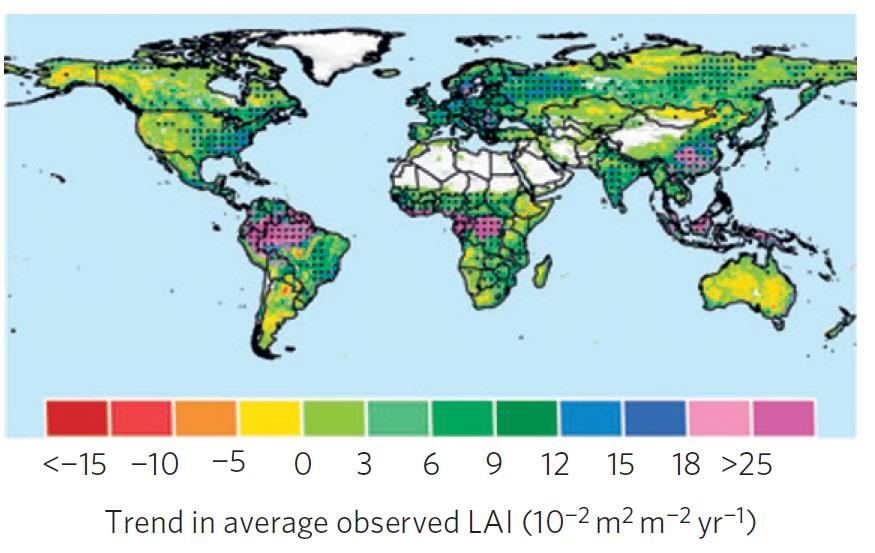
\includegraphics[width=1.0\textwidth]{bilder/bilderKlima-0002.jpg}\\[1cm]
\end{center}
\caption[]{Trends beim durchschnittlichen Blattflächenindex (LAI). Quelle: Zhu et al. 2016 Abbildung 3.}
\end{figure}

Piao et al. (2020) und Chen et al. (2024) berichten, dass der Ergrünungstrend ohne Anzeichen einer Verlangsamung fortsetzt, und CO$_2$-Düngung bleibt der dominante Treiber.

\subsection{Photosynthese und CO$_2$-Konzentrationen}

Pflanzen bauen Biomasse durch Photosynthese auf, einen Prozess, der Kohlendioxid, Wasser und Licht in Zucker umwandelt. Das für die Photosynthese verantwortliche Pflanzenenzym ist Ribulose-1,5-bisphosphat-carboxylase/oxygenase oder \emph{Rubisco}. Photosynthese wird eingeleitet, wenn CO$_2$ an der Oberfläche des Rubisco-Enzyms verfügbar ist, wo es in ein Molekül mit 3 Kohlenstoffatomen umgewandelt und danach in die Pflanzenmasse eingebaut wird. Dies wird als \emph{C3}-Prozess bezeichnet.

Rubisco wird geschätzt, vor etwa 3 Milliarden Jahren entstanden zu sein. Über geologische Zeit waren die atmosphärischen CO$_2$-Konzentrationen der Erde normalerweise viele Male höher als heute. Vor etwa 400 Millionen Jahren lagen CO$_2$-Konzentrationen schätzungsweise bei 2.000-4.000 ppm und waren für den größten Teil des Zeitraums von 200 bis 50 Millionen Jahren bei oder über 1.000 ppm (Berner 2006, Judd et al. 2024). Über die letzten 35 Millionen Jahre ist die atmosphärische CO$_2$-Konzentration stetig gefallen und fiel auf bis zu 170 ppm während Vereisung (Gerhart und Ward 2010). Während die moderne Änderungsrate von CO$_2$ im Vergleich zu früheren Zeiträumen hoch sein mag, zeigen die geologischen Beweise, dass Pflanzen und Tiere sich unter viel höheren CO$_2$-Konzentrationen als gegenwärtig entwickelten.

Als Antwort auf niedrige CO$_2$-Bedingungen entwickelten einige Pflanzen einen anderen photosynthetischen Weg namens \emph{C4}, bei dem CO$_2$ in der Nähe von Rubisco konzentriert wird, wodurch der \emph{C3}-Prozess effizienter funktionieren kann. Für landwirtschaftliche Zwecke sind die Pflanzenkategorien:
\begin{itemize}
\item C3: Reis, Weizen, Sojabohnen und die meisten anderen Feldfrüchte
\item C4: Mais, Zuckerrohr, Hirse, Sorghum	
\end{itemize}

Hätten atmosphärische CO$_2$-Konzentrationen weiter abgenommen, wäre das Pflanzenwachstum zurückgegangen und schließlich aufgehört. Unter \SI{180}{ppm} sind die Wachstumsraten vieler C3-Arten um 40-60 Prozent im Vergleich zu \SI{350}{ppm} reduziert (Gerhart und Ward 2010), und das Wachstum ist unter experimentellen Bedingungen von \SIrange{60}{140}{ppm} CO$_2$ vollständig zum Stillstand gekommen. Einige C4-Pflanzen können noch bei Konzentrationen von nur \SI{10}{ppm} wachsen, wenn auch sehr langsam (Gerhart und Ward 2010).


\begin{figure}[H]
\begin{center}
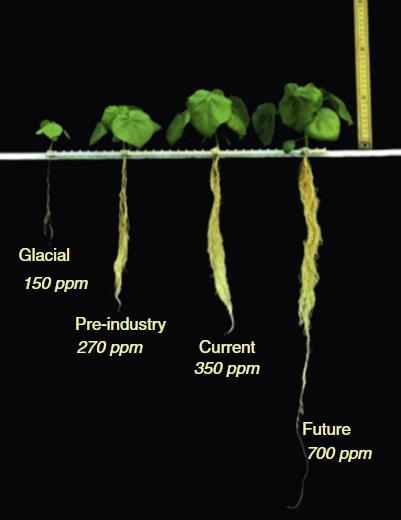
\includegraphics[width=0.7\textwidth]{bilder/bilderKlima-0003.jpg}\\[1cm]
\end{center}
\caption{Wachstum von \emph{Abutilon theophrasti} nach 14 Tagen unter identischen Bedingungen, jedoch mit den
angegebenen Schwankungen des CO2-Gehalts. Quelle: Gerhart und Ward (2010). Hinweis: „Aktuell” entspricht
1988 im Bild.}
\end{figure}

Die aktuellen CO$_2$-Konzentrationen liegen bei etwa \SI{430}{ppm}, gegenüber \SI{280}{ppm} in den frühen 1800er Jahren. Die positive Reaktion von Pflanzen auf zusätzliches CO$_2$ ist in Abbildung 2.2 dargestellt, reproduziert aus Gerhart und Ward (2010). Sie zeigt den Wachstumseffekt von CO$_2$ auf Samtpappel (Abutilon theophrasti) Sämlinge über 14 Tage unter kontrollierten Bedingungen, wo nur die CO$_2$-Exposition variiert wird. Die Zuwächse durch Erhöhung von CO$_2$ von \SI{150}{ppm} auf \SI{350}{ppm} setzen sich bei einer weiteren Verdopplung auf \SI{700}{ppm} fort.

Über die letzten 60+ Jahre gab es Tausende von Studien über die Reaktion von Pflanzen auf steigende CO$_2$-Konzentrationen. Das überwältigende Thema ist, dass Pflanzen, besonders C3-Pflanzen, von zusätzlichem CO$_2$ profitieren. Es gibt zwei Mechanismen, durch die CO$_2$ einen Wachstumsvorteil verleiht:

\begin{itemize}
\item Verstärkte Photosynthese über die oben beschriebenen Stoffwechselwege.
\item Erhöhte Wassernutzungseffizienz. Dies entsteht, weil Pflanzen CO$_2$ aufnehmen, indem sie die Stomata (Poren) auf der Blattoberfläche öffnen. Wenn CO$_2$ knapp ist, müssen die Stomata für lange Zeiträume weit offen gehalten werden, wodurch Wasser verdunsten kann. Unter angereicherten CO$_2$-Bedingungen bleiben die Stomata für längere Zeiträume geschlossen, wodurch die Pflanze Wasser länger zurückhalten kann und so die Wassernutzungseffizienz erhöht wird.
\end{itemize}

Spezifische Auswirkungen des Klimawandels auf die US-Landwirtschaft werden in Kapitel 9 überprüft.

\subsection{Steigendes CO$_2$ und Wassernutzungseffizienz von Feldfrüchten}

Deryng et al. (2016) untersuchten Beweise zur Wasserproduktivität von Feldfrüchten (CWP), dem Ertrag pro verwendete Wassereinheit, und lenkten Aufmerksamkeit auf das Potenzial von CO$_2$, sowohl die Photosynthese zu verstärken als auch die Transpiration auf Blattebene (Wasserverlust während der Blattatmung) zu reduzieren. Sie untersuchten alle verfügbaren FACE-Daten (Free Air CO$_2$ Enrichment—siehe Kapitel 9) zu Feldfruchtertragsänderungen für Mais, Weizen, Reis und Sojabohnen und kombinierten sie mit Feldfruchtemodell-Daten, die Ertragsreaktionen bis 2080 unter dem extremen RCP8.5-Emissionsszenario in vier Anbauregionen (Tropen, Trocken, Gemäßigt und Kalt) simulierten, von denen jede in regenabhängige und bewässerte Unterregionen aufgeteilt war. Sie berichteten, dass Modelle ohne CO$_2$-Düngung CWP-Verluste in jeder Region vorhersagten, aber diese wurden durch CO$_2$-Düngung mehr als ausgeglichen, sodass alle Regionen einen Netto-CWP-Gewinn zeigten.

Deryng et al. (2016) berichteten auch, dass negative Auswirkungen der Erwärmung auf Weizen- und Sojabohnenerträge vollständig durch CWP-Gewinne ausgeglichen und um bis zu 90 Prozent für Reis und 60 Prozent für Mais gemildert wurden.

Ähnlich bemerkten Cheng et al. (2017), dass die erhöhte Bruttoprimärproduktion von 1982 bis 2011 aufgrund steigender CO$_2$-Aufnahme von so großen CWP-Gewinnen begleitet war, dass der globale Wasserverbrauch von Pflanzen nicht gestiegen war, trotz der zusätzlichen Biomasse.

Deryng et al. (2016) nahmen an, dass Klimawandel \emph{Wasserknappheit verschärfen} würde. Doch während Modelle vorhersagen, dass Trockengebiete sich unter Klimaerwärmung ausdehnen werden, zeigen aktuelle Daten das Gegenteil: Ergrünung geschieht sogar in trockenen Gebieten. Zhang et al. (2024) berichten, dass aufgrund erhöhter CO$_2$-Konzentrationen \emph{zunehmende Trockenheit in Trockengebieten nicht zu einem allgemeinen Verlust der Vegetationsproduktivität führen wird}; höchstens 4 Prozent der derzeit trockenen Gebiete werden erhöhte Wüstenbildung erleben.

\subsection{CO$_2$-Düngungsvorteile in IPCC-Berichten}

Das IPCC hat globale Ergrünung und CO$_2$-Düngung landwirtschaftlicher Feldfrüchte nur minimal diskutiert. Das Thema wird kurz an einigen Stellen im Hauptteil des 6. und früherer IPCC-Bewertungsberichte anerkannt, aber in allen Zusammenfassungsdokumenten weggelassen. Abschnitt 2.3.4.3.3 des AR6 Working Group I-Berichts, betitelt \emph{globale Ergrünung und Bräunung}, weist darauf hin, dass der IPCC-Sonderbericht über Klimawandel und Land mit hoher Zuversicht geschlossen hatte, dass Ergrünung global über die letzten 2-3 Jahrzehnte zugenommen hatte. Er diskutiert dann, dass es Variationen im Ergrünungstrend zwischen Datensätzen gibt, und schließt, dass sie zwar hohe Zuversicht haben, dass Ergrünung aufgetreten ist, aber niedrige Zuversicht in das Ausmaß des Trends. Es gibt auch kurze Erwähnungen von CO$_2$-Düngungseffekten und Verbesserungen der Wassernutzungseffizienz in einigen anderen Kapiteln der AR6 Working Groups I und II-Berichte.

Insgesamt diskutieren jedoch die Policymaker Summaries, Technical Summaries und Synthesis Reports von AR5 und AR6 das Thema nicht.


\section{Die alkalischen Ozeane}

\subsection{Verändernder pH-Wert}

Eine neutrale wässrige Lösung hat einen pH-Wert von 7,0, während eine mit pH größer als 7,0 alkalisch (auch basisch genannt) und mit pH kleiner als 7,0 sauer ist. Der heutige globale Durchschnitts-pH-Wert von Oberflächenmeerwasser wird auf 8,04 geschätzt (\emph{Copernicus Marine Service 2025}, Abbildung 2.3), gegenüber einem geschätzten Wert von 8,2 in vorindustrieller Zeit (Gattuso und Hansson, 2011). Als CO$_2$-Konzentrationen in der Atmosphäre stiegen, absorbierten die Ozeane mehr, was ihren pH-Wert senkt. Abhängig von der Pufferkapazität der Ozeane wird erwartet, dass sie mit der Zeit etwas weniger alkalisch werden, was mit dem beobachteten pH-Rückgang übereinstimmt.

\begin{figure}[H]
\begin{center}
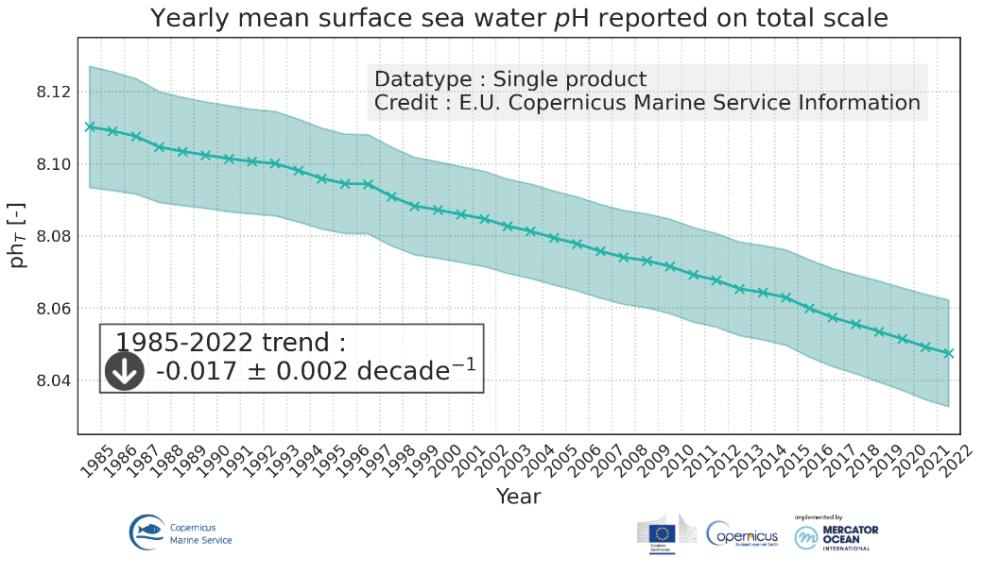
\includegraphics[width=1.0\textwidth]{bilder/bilderKlima-0004.jpg}\\[1cm]
\end{center}
\caption{pH-Wert der Ozeane 1985–2022. Quelle: Copernicus Marine Service 2025}
\end{figure}

Während dieser Prozess oft \emph{Ozeanversauerung} genannt wird, ist das eine Fehlbezeichnung, weil nicht erwartet wird, dass die Ozeane sauer werden; \emph{Ozeanneutralisierung} wäre genauer. Selbst wenn das Wasser sauer würde, wird angenommen, dass sich Leben in den Ozeanen entwickelte, als die Ozeane leicht sauer mit pH 6,5 bis 7,0 waren (Krissansen-Totton et al., 2018). Auf der Zeitskala von Tausenden von Jahren zeigen Bor-Isotop-Proxy-Messungen, dass der Ozean-pH-Wert während der letzten Vereisung (bis vor etwa 20.000 Jahren) um 7,4 oder 7,5 lag und auf heutige Werte anstieg, als sich die Welt während der Enteisung erwärmte (Rae et al., 2018). Somit scheinen Ozeanbiota widerstandsfähig gegenüber natürlichen langfristigen Veränderungen des Ozean-pH-Werts zu sein, da Meeresorganismen einer weiten Bandbreite von pH-Werten ausgesetzt waren.

\subsection{Korallenriff-Veränderungen}

Es gibt Bedenken, dass ein abnehmender pH-Wert des Meerwassers die Verkalkungsrate von Korallenriffen reduzieren wird. Aber Korallenriffe ertragen bereits große pH-Schwankungen, teilweise aufgrund täglicher photosynthetischer Aktivität im Riff; gemessene pH-Werte reichen von 9,4 während des Tages bis 7,5 nachts (Revelle und Fairbridge, 1957). De'ath et al. (2009) berichteten, dass Verkalkungsraten am Great Barrier Reef von 1990 bis 2005 um 14,2 Prozent zurückgegangen waren. Ridd et al. (2013) verwendeten jedoch andere Methoden und fanden keinen signifikanten Trend in den Verkalkungsraten.

Jüngste Daten vom Australian Institute of Marine Science zeigen, dass sich das Great Barrier Reef stark erholt hat. Der Korallenbedeckungsgrad erreichte 2022 36-Jahres-Höchststände in zwei Dritteln des Riffs. Das Institute kommentierte: \emph{Das war das dritte Jahr in Folge mit weit verbreiteter Erholung} (Australian Institute of Marine Science, 2022). Die \emph{Woods Hole Oceanographic Institution} bemerkte 2023: \emph{Das Great Barrier Reef macht ein bemerkenswertes Comeback} (Woods Hole Oceanographic Institution, 2023).

\begin{figure}[H]
\begin{center}
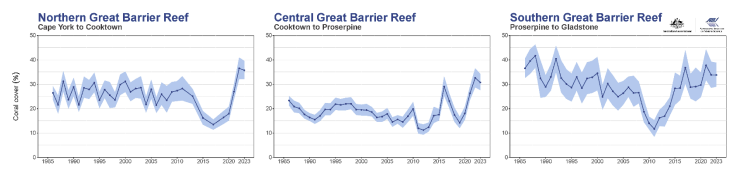
\includegraphics[width=1.0\textwidth]{bilder/bilderKlima-0005.png}\\[1cm]
\end{center}
\caption{Hartkorallenbedeckung in drei Regionen des \emph{Great Barrier Reef} von 1985 bis 2023. Quelle: AIMS 2023.}
\end{figure}

Es scheint, dass Korallen anpassungsfähiger sind als früher gedacht. Die Vorfahren moderner Korallen erschienen vor etwa 245 Millionen Jahren. CO$_2$-Konzentrationen waren für mehr als 200 Millionen Jahre danach viele Male höher als heute. Ein Großteil der öffentlichen Diskussion über die Auswirkungen der Ozean-"Versauerung" auf Meeresbiota war einseitig und übertrieben.

Ähnlich fand eine Meta-Analyse (Clements et al., 2021) der negativen Auswirkungen der Ozeanversauerung auf das Verhalten von Rifffischen das, was sie einen \emph{Decline-Effekt} nannten: anfänglich dramatische Schlussfolgerungen, die in prominenten Zeitschriften veröffentlicht wurden und scheinbar große Auswirkungen der Versauerung zeigten, tendierten dazu, von nachfolgenden Studien mit größeren Stichprobengrößen gefolgt zu werden, die viel kleinere und typischerweise nicht-existente Effekte ergaben. Sie fordern ihre Kollegen auf, Forschungspraktiken zu verbessern, um dem \emph{Decline-Effekt} entgegenzuwirken:

Die überwiegende Mehrheit der Studien mit großen Effektgrößen in diesem Bereich tendiert dazu, durch niedrige Stichprobengrößen charakterisiert zu sein, wird aber dennoch in hochrangigen Zeitschriften veröffentlicht und hat einen unverhältnismäßigen Einfluss auf das Feld in Bezug auf Zitationen. Wir behaupten, dass Ozeanversauerung einen vernachlässigbaren direkten Einfluss auf Fischverhalten hat, und wir setzen uns für verbesserte Ansätze ein, um das Potenzial für einen Decline-Effekt in zukünftigen Forschungsrichtungen zu minimieren (Clements et al., 2021).

Zusammenfassend ist Meeresleben komplex, und vieles davon entwickelte sich, als die Ozeane relativ zur Gegenwart sauer waren. Die Vorfahren moderner Korallen erschienen vor etwa 245 Millionen Jahren. CO$_2$-Konzentrationen waren für mehr als 200 Millionen Jahre danach viele Male höher als heute. Ein Großteil der öffentlichen Diskussion über die Auswirkungen der Ozean-"Versauerung" auf Meeresbiota war einseitig und übertrieben.

\vfill
\noindent\textbf{Literaturverzeichnis:}

\begingroup
\parindent=0pt
\everypar{\hangindent=2em\hangafter=1\relax}

AR6: Intergovernmental Panel on Climate Change Sixth Assessment Report (2021) Working Group I Contribution. www.ipcc.ch.

Australian Institute of Marine Science. (2022). Continued coral recovery leads to 36-year highs across two-thirds of the Great Barrier Reef. \url{https://www.aims.gov.au/sites/default/files/2022-08/AIMS_LTMP_Report_on\%20GBR_coral_status_2021_2022_040822F3.pdf}

Beeden, R., Maynard, J., Puotinen, M., Marshall, P., Dryden, J., Goldberg, J., and Williams, G. (2015). Impacts and recovery from Severe Tropical Cyclone Yasi on the Great Barrier Reef. PLOS ONE, 10, e0121272. https://doi.org/10.1371/journal.pone.0121272

Berner, R. A. (2006). GEOCARBSULF: A combined model for Phanerozoic atmospheric O$_2$ and CO$_2$. Geochimica et Cosmochimica Acta, 70, 5653–5664.

Browman, H. I. (2016). Applying organized scepticism to ocean acidification research. ICES Journal of Marine Science, 73(3), 529.1–536. https://doi.org/10.1093/icesjms/fsw010

Chen, C., Park, T., Wang, X., Piao, S., Xu, B., Chaturvedi, R. K., and Myneni, R. B. (2019). China and India lead in greening of the world through land-use management. Nature Sustainability, 2, 122–129. https://www.nature.com/articles/s41893-019-0220-7

Chen, X., Wang, Y., Liu, Y., and Piao, S. (2024). The global greening continues despite increased drought stress since 2000. Global Ecology and Conservation, 49, e02791. https://www.sciencedirect.com/science/article/pii/S2351989423004262

Cheng, L., Zhang, L., Wang, Y. P., et al. (2017). Recent increases in terrestrial carbon uptake at little cost to the water cycle. Nature Communications, 8, 110. https://doi.org/10.1038/s41467-017-00114-5

Clements, J. C., Sundin, J., Clark, T. D., and Jutfelt, F. (2022). Meta-analysis reveals an extreme "decline effect" in the impacts of ocean acidification on fish behavior. PLOS Biology, 20(2), e3001511. https://doi.org/10.1371/journal.pbio.3001511

Copernicus Marine Service. (2025). Global ocean acidification – Mean sea water pH time series and trend from multi-observations reprocessing. \url{https://data.marine.copernicus.eu/product/GLOBAL_OMI_HEALTH_carbon_ph_area_averaged/description}

De'ath, G., Lough, J., and Fabricius, K. (2009). Declining coral calcification on the Great Barrier Reef. Science, 323, 116–119. https://doi.org/10.1126/science.1165283

Deryng, D., Conway, D., Ramankutty, N., Price, J., Warren, R., Jones, R., ... and Elliott, J. (2016). Regional disparities in the beneficial effects of rising CO$_2$ concentrations on crop water productivity. Nature Climate Change. https://doi.org/10.1038/nclimate2995

Gattuso, J. P., and Hansson, L. (Eds.). (2011). Ocean acidification: Background and history. Oxford University Press.

Gerhart, L. M., and Ward, J. K. (2010). Plant responses to low [CO$_2$] of the past. New Phytologist, 188, 674–695. https://nph.onlinelibrary.wiley.com/doi/pdf/10.1111/j.1469-8137.2010.03441.x

Haverd, V., B. Smith, J. G. Canadell, et al. (2020). Higher than expected CO$_2$ fertilization inferred from leaf to global observations. Global Change Biology, 26, 2390–2402. https://doi.org/10.1111/gcb.14950

Keenan, T. F., X. Luo, B. D. Stocker, et al. (2023). A constraint on historic growth in global photosynthesis due to rising CO2. Nature Climate Change 13(12): 1376-1381 DOI: 10.1038/s41558-023-01867-2.

Judd, E. J., Scotese, C. R., Young, S. A., et al. (2024). A 485-million-year history of Earth's surface temperature. Science, 385(6715). https://doi.org/10.1126/science.adk3705

Krissansen-Totton, J., Arney, G. N., and Catling, D. C. (2018). Constraining the climate and ocean pH of the early Earth with a geological carbon cycle model. Proceedings of the National Academy of Sciences, 115(6), 4105–4110. https://doi.org/10.1073/pnas.1721296115

Piao, S., X. Wang, T. Park, et al. (2020). Characteristics, drivers and feedbacks of global greening. Nature Reviews Earth \& Environment 1(1): 14-27 DOI: 10.1038/s43017-019-0001-x

Rae, J. W. B., Burke, A., Robinson, L. F., et al. (2018). CO$_2$ storage and release in the deep Southern Ocean on millennial to centennial timescales. Nature, 562, 569–573. https://doi.org/10.1038/s41586-018-0614-0

Revelle, R., and Fairbridge, R. W. (1957). Carbonate and carbon dioxide. In J. W. Hedgpeth (Ed.), Treatise on marine ecology and paleoecology (Vol. 1). Geological Society of America.

Ridd, P., Silva, E., and Stieglitz, T. (2013). Have coral calcification rates slowed in the last twenty years? Marine Geology, 346, 392–399. https://doi.org/10.1016/j.margeo.2013.09.002

Woods Hole Oceanographic Institution. (2023). Is the Great Barrier Reef making a comeback? https://www.whoi.edu/oceanus/feature/is-the-great-barrier-reef-making-a-comeback/

Zeng, Z., Piao, S. Li, L., et al. (2017). Climate mitigation from vegetation biophysical feedbacks during the past three decades. Nature Climate Change. https://doi.org/10.1038/nclimate3299

Zhang, Y., Liu, Y., Chen, X., et al. (2024). Less than 4% of dryland areas are projected to desertify despite increased aridity under climate change. Nature Communications Earth and Environment, 5. https://www.nature.com/articles/s43247-024-01463-y

Zhu, Z., Piao, S., Myneni, R. B., et al. (2016). Greening of the Earth and its drivers. Nature Climate Change, 6, 791–795. https://www.nature.com/articles/nclimate3004
\endgroup

%\numberwithin{figure}{section}
\FigureNumbersBySection
\chapter{Menschliche Einflüsse auf das Klima}
\paragraph{Kapitelzusammenfassung}
\begin{quote}
Das globale Klima ist natürlicherweise auf allen Zeitskalen variabel. Anthropogene CO$_2$-Emissionen verstärken diese Variabilität, indem sie die gesamte Strahlungsenergiebilanz in der Atmosphäre verändern.

Das IPCC hat die Rolle der Sonne beim Klimawandel herabgespielt, aber es gibt plausible Rekonstruktionen der Sonneneinstrahlung, die darauf hindeuten, dass sie zur jüngsten Erwärmung beigetragen hat.

Klimaprojektionen basieren auf IPCC-Emissionsszenarien, die dazu tendierten, beobachtete Trends zu übertreffen. Die meisten akademischen Klimaauswirkungsstudien der letzten Jahre basieren auf dem extremen RCP 8.5-Szenario, das jetzt als unplausibel gilt; seine Verwendung als Business-as-usual-Szenario war irreführend.

Kohlenstoffkreislaufmodelle verbinden jährliche Emissionen mit dem Wachstum des atmosphärischen CO$_2$-Bestands. Während sich Modelle über die Rate der Land- und Ozean-CO$_2$-Aufnahme uneinig sind, stimmen alle darin überein, dass sie seit 1959 gestiegen ist.

Es gibt Belege dafür, dass Urbanisierungsverzerrungen in der Landerwärmungsaufzeichnung nicht vollständig aus Klimadatensätzen entfernt wurden.
\end{quote}

\section{Komponenten der Strahlungsantriebe und ihre Geschichte}
\subsection{Historischer Strahlungsantrieb}
Ein sich veränderndes Klima war die Norm während der gesamten 4.6 Milliarden Jahre langen Geschichte der Erde. Die Temperatur und Wettermuster der Erde verändern sich natürlich über Zeitskalen von Jahrzehnten bis zu Millionen von Jahren. Natürliche Variationen des Oberflächenklimas entstehen auf zwei Wegen. Interne Klimaschwankungen im Zusammenhang mit Zirkulationen in der Atmosphäre und den Ozeanen tauschen Energie, Wasser und Kohlenstoff zwischen der Atmosphäre, Ozeanen, Land und Eis aus. Externe Einflüsse auf das Klimasystem umfassen Variationen in der von der Sonne empfangenen Energie und die Auswirkungen von Vulkanausbrüchen. Menschliche Aktivitäten beeinflussen das Klima durch Veränderungen der Landnutzung und Landbedeckung. Menschen verändern auch die Zusammensetzung der Atmosphäre durch Emissionen von CO$_2$ und anderen Treibhausgasen und durch die Veränderung der Konzentration von Aerosolpartikeln in der Atmosphäre.

Die Erde wird durch das Sonnenlicht erwärmt, das sie absorbiert, und wird durch die Wärme gekühlt, die sie in den Weltraum abstrahlt. Über die Erdoberfläche gemittelt, beinhalten diese Prozesse jeweils Energieflüsse von etwa 240 Watt pro Quadratmeter (W/m²). Wenn sie im Gleichgewicht sind, gibt es keine äußeren Ursachen für Erwärmung oder Abkühlung. Sowohl menschliche als auch natürliche Einflüsse auf das Klima verändern dieses Gleichgewicht und verursachen damit Klimaveränderungen.

Einflüsse auf die Energiebilanz der Erde an der Spitze der Atmosphäre werden durch \emph{Strahlungsantrieb} quantifiziert, das Ausmaß, in dem sie das Erwärmungs-/Abkühlungsgleichgewicht stören; ein positiver Antrieb erwärmt, während ein negativer Antrieb kühlt. Die geschätzte Geschichte der wichtigsten Komponenten des Strahlungsantriebs seit 1750 durch das IPCC ist in den folgenden zwei Abbildungen aus seinem AR6 dargestellt.

\begin{figure}[H]
\begin{center}
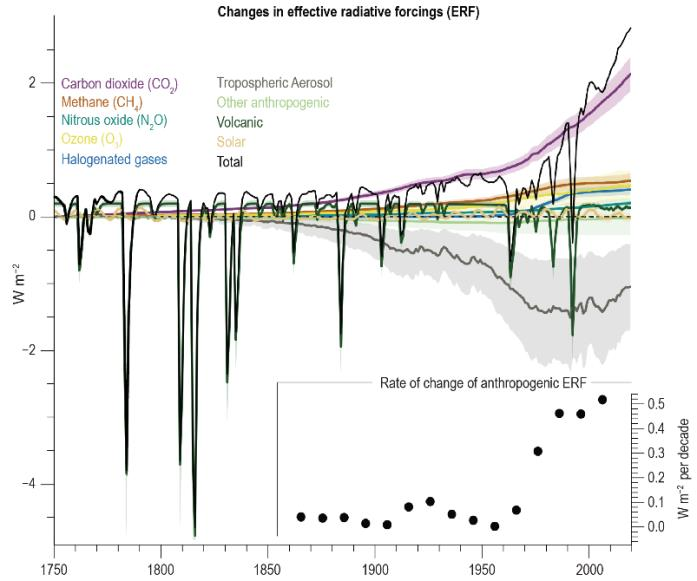
\includegraphics[width=1.0\textwidth]{bilder/bilderKlima-0006.jpg}\\[1cm]
\end{center}
\caption{IPCC-Schätzungen der Komponenten des Strahlungsantriebs im Zeitverlauf. Die Schattierung zeigt
die Unsicherheitsbereiche an. Quelle: AR6 WGI Ch2 Abb. 10}
\end{figure}

\begin{figure}[H]
\begin{center}
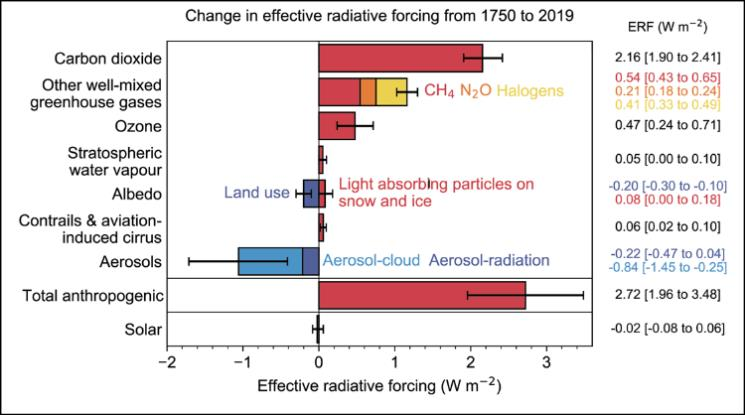
\includegraphics[width=1.0\textwidth]{bilder/bilderKlima-0007.jpg}\\[1cm]
\end{center}
\caption{IPCC-Schätzungen der Veränderungen der Strahlungsantriebskomponenten von 1750 bis 2019. Quelle:
AR6 WGI Kap. 7 Abb. 7-6.}
\end{figure}

Diese Grafiken zeigen, dass der gesamte Strahlungsantrieb sowohl aus natürlichen als auch aus anthropogenen Komponenten besteht. Kohlendioxid ist der größte menschliche Einfluss auf das Klima und derjenige, der am relevantesten für den Einfluss der Nutzung fossiler Brennstoffe ist. Es übt einen erwärmenden Einfluss aus, indem es die Kühlkraft der Atmosphäre verringert. CO$_2$-Emissionen akkumulieren in der Atmosphäre, wie im folgenden Abschnitt beschrieben, sodass der erwärmende Einfluss wächst.

Andere anthropogene Strahlungsantriebe umfassen andere Treibhausgase (Methan, Lachgas, fluorierte Gase), Aerosole und Landnutzungsänderungen. Es gibt jedoch erhebliche Unsicherheiten in diesen Komponenten. Das IPCC identifiziert Wolken-Aerosol-Wechselwirkungen als die größte Unsicherheit im gesamten Strahlungsantrieb.

Eine wichtige natürliche Komponente ist die Sonneneinstrahlung. Variationen in der Sonnenaktivität sind gut dokumentiert und können das Klima beeinflussen. Das IPCC hat jedoch die Rolle solarer Variabilität beim Klimawandel heruntergespielt. Soon et al. (2021) stellten fest, dass die Konsensaussagen des IPCC zum solaren Antrieb vorzeitig durch die Unterdrückung abweichender wissenschaftlicher Meinungen formuliert wurden.

Eine weitere natürliche Strahlungsantriebskomponente sind vulkanische Aerosole, die einen episodischen kühlenden Einfluss ausüben. Box 4.1 im IPCC AR6-Bericht behandelt die Klimaauswirkungen von Vulkanausbrüchen und bemerkt drei explosive Vulkanausbrüche, die in der ersten Hälfte des 19. Jahrhunderts auftraten. Dazu gehörte der Tambora-Ausbruch von 1815, der zum 'Jahr ohne Sommer' führte, mit mehreren Ernteausfällen in der gesamten Nordhalbkugel. Es gibt Unsicherheit über das Vorzeichen der relativ kleinen Antriebskraft des Unterwasservulkans Hunga Tonga, der 2022 ausbrach (Jenkins et al. 2023, Schoeberl et al. 2024).

Abbildung 3.1.1 zeigt, dass die anthropogene Antriebskomponente vor etwa 1900 vernachlässigbar war und seitdem stetig gestiegen ist und heute auf fast \SI{3}{\watt\per\square\meter} angestiegen ist. Dies ist jedoch immer noch nur etwa 1 Prozent der ungestörten Strahlungsflüsse, was es zu einer Herausforderung macht, die Auswirkungen des anthropogenen Antriebs zu isolieren; modernste Satellitenschätzungen globaler Strahlungsenergieflusse sind nur auf wenige \si{\watt\per\square\meter} genau.

Natürliche Quellen globaler Energieungleichgewichte außer Vulkanen und der gesamten Sonneneinstrahlung (TSI) sind in diesen Grafiken nicht enthalten, da sie weitgehend unbekannt bleiben.

\subsection{Veränderung des atmosphärischen CO$_2$ seit 1958}

Der erwärmende Einfluss von Kohlendioxid hängt davon ab, wie viel \emph{zusätzliches} CO$_2$ sich in der Atmosphäre ansammelt – d.h. seine Konzentration über dem vorindustriellen Wert von \SI{280}{ppm}. Der CO$_2$-Gehalt, wie er am Mauna Loa-Observatorium in Hawaii aufgezeichnet wird, der allgemein als repräsentative globale Durchschnittskonzentration verwendet wird, ist online verfügbar unter \url{https://gml.noaa.gov/ccgg/trends/index.html}. Die Konzentration lag zu Beginn der Aufzeichnung 1959 bei etwa \SI{316}{ppm} und liegt jetzt bei etwa \SI{430}{ppm}, ein Anstieg von 36 Prozent. Am Ende der letzten Vereisung waren die CO$_2$-Konzentrationen auf etwa \SI{180}{ppm} gefallen. Wie in Kapitel 2 diskutiert, beginnen C3-Pflanzen bei CO$_2$-Konzentrationen unter etwa \SI{140}{ppm} zu sterben und C4-Pflanzen bei Konzentrationen unter \SI{100}{ppm}, sodass bei weiterem Fallen der CO$_2$-Konzentrationen das Pflanzenleben gefährdet gewesen wäre.


\begin{figure}[H]
\begin{center}
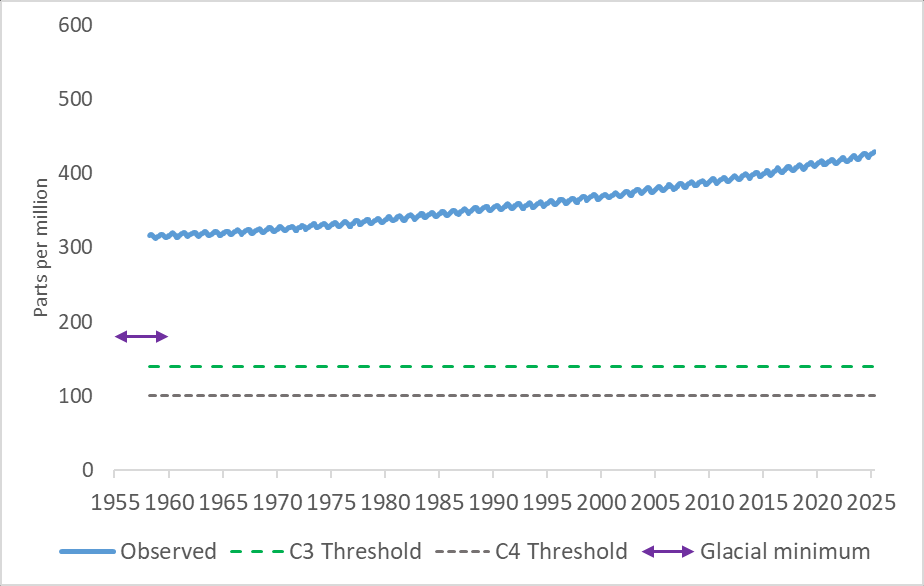
\includegraphics[width=1.0\textwidth]{bilder/bilderKlima-0009.png}\\[1cm]
\end{center}
\caption{Jährliche durchschnittliche CO2-Konzentrationen in der Atmosphäre (1959–2025) in ppm, gemessen am
Mauna Loa (blau). C3-Schwellenwert: Wert, unterhalb dessen C3-Pflanzen zu sterben beginnen (140 ppm, siehe
Kapitel 2). C4-Schwellenwert: Wert, unterhalb dessen C4-Pflanzen zu sterben beginnen (100 ppm, siehe Kapitel 2).
Glaziales Minimum: Mindestniveau während der letzten Eiszeiten (lila Pfeil). CO2-Datenquelle:
\url{https://gml.noaa.gov/ccgg/trends/index.html}}
\end{figure}

Der jährliche Konzentrationsanstieg ist nur etwa die Hälfte des emittierten CO$_2$, weil Land- und Ozeanprozesse derzeit \emph{überschüssiges} CO$_2$ mit einer Rate von etwa 50 Prozent der menschlichen Emissionen absorbieren. Zukünftige Konzentrationen und damit zukünftige menschliche Einflüsse auf das Klima hängen daher von zwei Komponenten ab: (1) zukünftige Raten globaler menschlicher CO$_2$-Emissionen und (2) wie schnell Land und Ozean zusätzliches CO$_2$ aus der Atmosphäre entfernen. Wir diskutieren jede dieser der Reihe nach.

\section{Zukünftige Emissionsszenarien und der Kohlenstoffkreislauf}

\subsection{Emissionsszenarien}

Die Bewertung der Gefahren zukünftiger THG-Emissionen erfordert Annahmen darüber, was diese Emissionen sein werden. Zukünftige Emissionen und damit menschliche Einflüsse auf das Klima werden von zukünftiger Demografie, Wirtschaftstätigkeit, Regulierung sowie Energie- und Agrartechnologien abhängen. Verschiedene Annahmen über jeden dieser Faktoren führen zu Projektionen von Treibhausgasemissionen und -konzentrationen, Aerosolkonzentrationen und Veränderungen der Landnutzung, die letztendlich zu Annahmen über anthropogenen Strahlungsantrieb kombiniert werden können.

Die großen Unsicherheiten über diese vielen Faktoren machen es unmöglich, zukünftige Emissionen präzise vorherzusagen. Stattdessen hat das IPCC verschiedene Szenario-Sets verwendet, die einen plausiblen Bereich von Möglichkeiten für Bevölkerung, Wirtschaft und Technologien abdecken sollen. Jüngste Versionen der Szenarien sind durch eine Zahl gekennzeichnet, die den anthropogenen Strahlungsantrieb angibt, der 2100 unter diesem Szenario erwartet wird. So entspricht ein mit "6" bezeichnetes Szenario \SI{6}{\watt\per\square\meter} menschlich induziertem Strahlungsantrieb (Erwärmung) am Ende des Jahrhunderts. (Erinnern Sie sich, der aktuelle anthropogene Strahlungsantrieb beträgt etwa \SI{2.7}{\watt\per\square\meter}.)

Obwohl das IPCC nicht behauptet, dass seine Emissionsszenarien Vorhersagen sind, werden sie oft als solche behandelt. Vergleiche vergangener Szenario-Gruppen mit Beobachtungen zeigen, dass IPCC-Emissionsprojektionen dazu tendierten, tatsächliche nachfolgende Emissionen zu überschätzen. Für den dritten und vierten IPCC-Bewertungsbericht wurde eine Reihe von Emissionsprojektionen aus dem Sonderbericht zu Emissionsszenarien verwendet; diese wurden als SRES-Szenarien bezeichnet. McKitrick et al. (2012) zeigten, dass die SRES-Szenario-Emissionsverteilung bei Umrechnung in Pro-Kopf-Werte im Vergleich zu beobachteten Trends nach oben verzerrt war. Die Verzerrung der SRES-Szenarien wurde durch die spätere Analyse von Hausfather et al. (2019) bestätigt, die zeigten, dass beobachtete atmosphärische CO$_2$-Konzentrationen dem unteren Ende des SRES-Bereichs und auch nachfolgender IPCC-Szenario-Bereiche folgten (Abbildung 3.2.1).

Für AR5 entwickelte das IPCC ein neues Set von Szenarien, die \emph{Representative Concentration Pathways} (RCPs) genannt wurden. Diese wurden durch eine Zahl identifiziert, die den Anstieg im Antrieb repräsentierte, und wurden daher RCP2.6, RCP4.5, RCP6.0 und RCP8.5 genannt. RCP2.6 (was einen anthropogenen Strahlungsantrieb 2100 von \SI{2.6}{\watt\per\square\meter} impliziert) beschreibt einen THG-Konzentrationspfad, der zu einer Erwärmung deutlich unter 2°C führt. Am anderen Ende der Skala ist RCP8.5 ein extremes Ergebnis, das fast \SI{5}{\celsius} Erwärmung von 1900 bis 2100 impliziert.

RCP8.5 kam dazu, als \emph{No-Policy-Baseline} oder \emph{Business-as-usual}-Szenario sowohl in der akademischen Literatur als auch in den populären Medien bezeichnet zu werden. Es wurde daher verwendet, um das Referenzergebnis zu generieren, das angeblich die Welt des 21. Jahrhunderts in Abwesenheit zunehmend strenger Emissionsreduktionspolitiken repräsentiert. Aber RCP8.5 war als ein Niedrig-Wahrscheinlichkeits-Hochemmissionsszenario gedacht, und seine Verwendung als Business-as-usual-Baseline wurde als grob irreführend kritisiert.\footnote{Dieses extreme Szenario ist nützlich für Modellierer, da ein großer Antrieb eine große Antwort (Erwärmung) generiert, was es einfacher macht, die Sensitivität eines Modells zu bewerten. Aber das ist sehr unterschiedlich davon, zu behaupten, es sei ein plausibles zukünftiges Ergebnis.} Hausfather und Peters (2020a), die in einem Kommentar in Nature schrieben, wiesen darauf hin, dass RCP8.5 als ein extremer Worst-Case entwickelt wurde, und sein Missbrauch als \emph{Business as usual}-Baseline hat zu einer großen Anzahl irreführender Studien und Medienberichterstattung geführt.

Die Unplausibilität des RCP8.5-Szenarios wurde von Burgess et al. (2021) untersucht. Die Unplausibilität von RCP8.5 sollte nicht als sehr unwahrscheinlich (z.B. 95. Perzentil) oder ein \emph{Worst Case} interpretiert werden, sondern eher als genuinen unplausibel aufgrund der Unplausibilität der Inputs, die erforderlich sind, um einen Antrieb von \SI{8.5}{\watt\per\square\meter} zu erreichen. Sie bemerkten, dass RCP8.5 bereits von beobachteten Trends in der Energienutzung abgewichen ist und die nahen zukünftigen Trends scharf von denen der Internationalen Energieagentur (IEA) abweichen, die marktbasierte Projektionen der Energienutzung für die kommenden Jahrzehnte bereitstellt. Pielke Jr. et al. (2022) zeigten weiter, dass die historischen und projizierten IEA-Trends nahe dem Boden der Umhüllungen sowohl der RCP-Projektionen als auch der jüngeren Shared Socioeconomic Pathway (SSP)-Szenario-Trends verlaufen.

Schwalm et al. (2020) verteidigten die Verwendung von RCP8.5 mit der Begründung, dass kumulative CO$_2$-Emissionen über 2005-2020 es enger verfolgen als die niedrigeren RCP-Szenarien. Sie argumentieren auch, dass eine modifizierte Version der IEA-Szenarien RCP8.5 in den kommenden Jahrzehnten eng verfolgt. Hausfather und Peters (2020b) antworteten, dass die Fertigkeit von RCP8.5 über diese 15 Jahre auf ausgleichende Fehler in seiner Repräsentation von CO$_2$ aus Brennstoffnutzung und Landnutzungsänderung zurückzuführen ist, und die scheinbare Übereinstimmung mit IEA in kommenden Jahrzehnten ist darauf zurückzuführen, dass Schwalm et al. sehr hohe Landnutzungsemissionen hinzufügten. Die eigenen projizierten CO$_2$-Emissionen der IEA verfolgen deutlich unter RCP8.5.

Weitverbreitete Verwendung von RCP8.5 als No-Policy-Baseline hat eine Verzerrung in Richtung Alarm in der Klimaauswirkungsliteratur geschaffen. Das Ausmaß dieses Problems wurde in einer Literaturanalyse von Pielke Jr. und Ritchie (2020) bestätigt. Sie fanden, dass etwa 16.800 wissenschaftliche Arbeiten, die zwischen 2010 und 2020 veröffentlicht wurden, das RCP8.5-Szenario verwendeten, wobei etwa 4.500 der Artikel RCP8.5 mit dem Konzept von \emph{Business-as-usual} verknüpften. Ihre Analyse zeigte, wie RCP8.5 nicht nur von einzelnen Forschern missbraucht wurde, sondern auch von einflussreichen Wissenschaftsagenturen wie dem IPCC und dem U.S. National Climate Assessment (USNCA), was direkt zu irreführender Berichterstattung in prominenten Medien geführt hat.

\begin{figure}[H]
\begin{center}
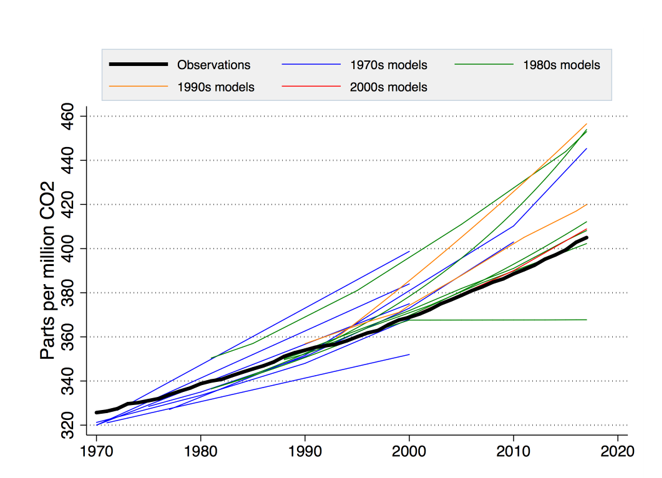
\includegraphics[width=1.0\textwidth]{bilder/bilderKlima-0011.png}\\[1cm]
\end{center}
\caption{Seit den 1970er Jahren haben aufeinanderfolgende Familien von Emissions- und Konzentrationsprognosen (farbige
Linien) die Beobachtungen (schwarze Linie) durchweg überschätzt. Quelle: Hausfather et al. (2019)
Abbildung S4.}
\end{figure}

Pielke und Ritchie (2020) berichteten, dass neue Studien, die RCP8.5 verwendeten, mit einer Rate von etwa 20 pro Tag veröffentlicht wurden, wobei etwa zwei pro Tag spezifisch RCP8.5 und \emph{business as usual} verknüpften. Sie schließen, dass die Klimaforschungsgemeinschaft ein Jahrzehnt damit verbracht hat, \emph{wissenschaftliche Ressourcen für Science Fiction zu verwenden} und dass \emph{Die wissenschaftliche Literatur ist in eine apokalyptische Richtung unausgewogen geworden.}

Das IPCC entwickelte ein neues Set von Szenarien für AR6, die \emph{Shared Socioeconomic Pathway} (SSP)-Szenarien, die die in den RCP- und SRES-Szenarien gezeigte Verzerrung fortgesetzt haben. Abbildung 3.2.2 zeigt die von der Internationalen Energieagentur (IEA) zusammengestellten gesamten globalen beobachteten CO$_2$-Emissionen, zusammengeführt mit der Emissionsprojektion der EIA unter Berücksichtigung von Energienutzungsprojektionen und aktuellen Politiken. Die anderen Linien zeigen den Bereich der IPCC SSP-Szenarien (SSP1-SSP5). Ab 2023 lagen globale CO$_2$-Emissionen deutlich unter SSP7.0 und waren sogar unter SSP2-4.5.

\begin{figure}[H]
\begin{center}
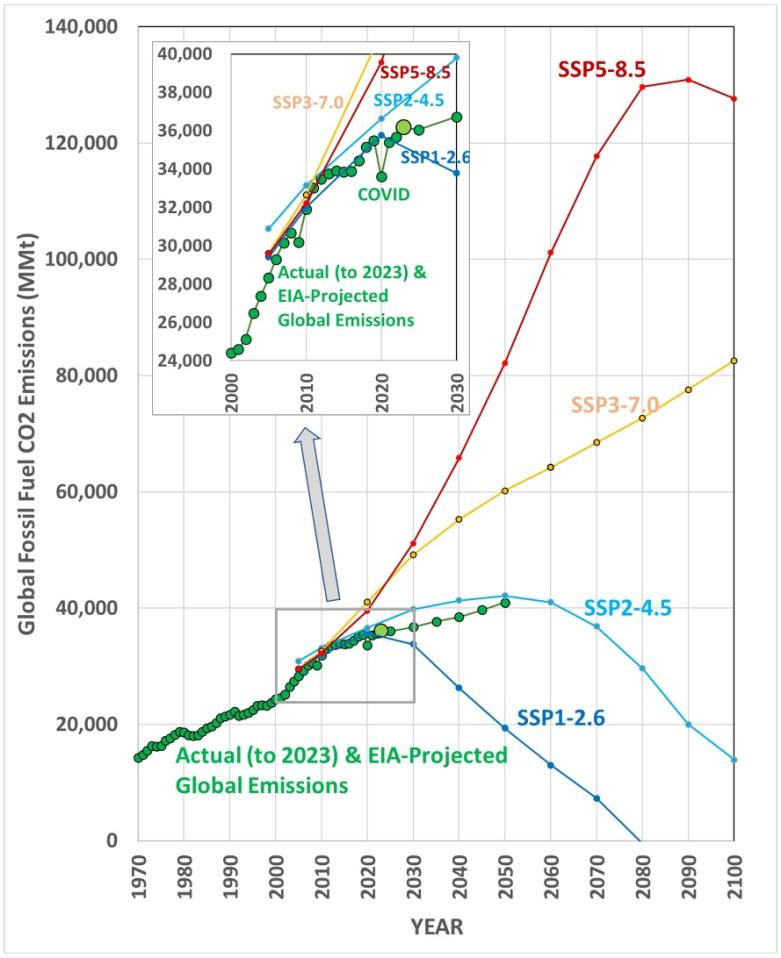
\includegraphics[width=1.0\textwidth]{bilder/bilderKlima-0012.jpg}\\[1cm]
\end{center}
\caption{Beobachtete und prognostizierte CO$_2$-Emissionen. Quelle: IPCC (SSP-Szenarien) und
Energy Information Administration (EIA). Grün: beobachtete historische Emissionen und EIA-Prognosen.
Andere Linien: SSP1-5. Datenquelle: Friedlingstein et al. (2024).}
\end{figure}

\subsection{Der Kohlenstoffkreislauf, der Emissionen und Konzentrationen in Beziehung setzt}
Kohlendioxidemissionen aus der Verbrennung fossiler Brennstoffe (und in geringerem Maße Entwaldung und Zementproduktion) haben zu stetig steigenden CO$_2$-Konzentrationen in der Atmosphäre geführt, wie in Abb. 3.1.3 gezeigt. Die Beziehung zwischen Emissionen und Konzentration wird durch den globalen Kohlenstoffkreislauf von Land- und Ozeanprozessen bestimmt, die Kohlenstoff mit der Atmosphäre austauschen. Unser Verständnis dieser Prozesse wurde von Crisp et al. (2021) überprüft.

Es gibt etwa \SI{850}{\giga\tonne} Kohlenstoff (\si{\giga\tonne\of{C}}) in der Erdatmosphäre\footnote{Weil CO$_2$ chemisch durch den Verlauf des Kohlenstoffkreislaufs transformiert wird, ist es zweckmäßiger, Kohlenstoffatome zu verfolgen statt CO$_2$-Moleküle. Eine Gigatonne Kohlenstoff (\si{\giga\tonne\of{C}}) entspricht etwa \SI{3.7}{\giga\tonne} CO$_2$.}, fast alles davon in der Form von CO$_2$. Jedes Jahr tauschen biologische Prozesse (Pflanzenwachstum und -zerfall) und physische Prozesse (Ozeanabsorption und -ausgasung) etwa \SI{200}{\giga\tonne\of{C}} dieses Kohlenstoffs mit der Erdoberfläche aus (ungefähr \SI{80}{\giga\tonne\of{C}} mit dem Land und \SI{120}{\giga\tonne\of{C}} mit den Ozeanen). Bevor menschliche Aktivitäten bedeutsam wurden, waren Entfernungen aus der Atmosphäre grob im Gleichgewicht mit Hinzufügungen. Aber die Verbrennung fossiler Brennstoffe (Kohle, Öl und Gas) entfernt Kohlenstoff aus dem Boden und fügt ihn dem jährlichen Austausch mit der Atmosphäre hinzu. Diese Hinzufügung (zusammen mit einem viel kleineren Beitrag aus der Zementherstellung) belief sich 2023 auf \SI{10.3}{\giga\tonne\of{C}} oder nur etwa 5 Prozent des jährlichen Austauschs mit der Atmosphäre.

Der Kohlenstoffkreislauf nimmt etwa 50 Prozent der kleinen jährlichen Injektion von Kohlenstoff der Menschheit in die Luft auf, indem er ihn natürlich durch Pflanzenwachstum und ozeanische Aufnahme sequestriert, während der Rest sich in der Atmosphäre ansammelt (Ciais et al., 2013). Aus diesem Grund beträgt der jährliche Anstieg der atmosphärischen CO$_2$-Konzentration im Durchschnitt nur etwa die Hälfte dessen, was naiv von menschlichen Emissionen erwartet würde.

Um zukünftige CO$_2$-Konzentrationen in der Atmosphäre und damit zukünftige menschliche Einflüsse auf das Klima zu projizieren, ist es wichtig zu wissen, wie sich der Kohlenstoffkreislauf in der Zukunft ändern könnte. Die historische Beinahe-Konstanz dieses 50-Prozent-Anteils bedeutet, dass je mehr CO$_2$ die Menschheit produziert hat, desto schneller hat die Natur es aus der Atmosphäre entfernt. Dieser 50-Prozent-Anteil ändert sich von Jahr zu Jahr etwas aufgrund natürlicher Kohlenstoffkreislauf-Ungleichgewichte durch El Ni\~no, La Ni\~na und variierende Wettermuster. Es gab auch eine erhebliche zusätzliche Reduktion des atmosphärischen CO$_2$ nach dem Ausbruch des Mount Pinatubo 1991, ein merkwürdiges Ergebnis, das noch erklärt werden muss (Angert et al., 2004).

Die Hauptprozesse, die überschüssiges CO$_2$ aus der Atmosphäre entfernen, sind verstärktes Wachstum der Landvegetation (besonders in hohen Breitengraden), eine gewisse Zunahme der Kohlenstoffsequestrierung in Böden und die Aufnahme von CO$_2$ durch den Ozean aufgrund des steigenden Partialdrucks von atmosphärischem CO$_2$ gegenüber dem in den Ozeanen gelösten CO$_2$. Alle zwanzig Landkohlenstoffkreislauf-Modelle, die vom Global Carbon Project verfolgt werden (Friedlingstein et al., 2024), zeigen, dass Landprozesse seit 1959 überschüssiges CO$_2$ mit steigender Rate entfernen. Dies stimmt mit einem \emph{globalen Ergrünungs}-Phänomen (Kapitel 2.1) überein, das von Satelliten seit Beginn der Überwachung der globalen Grünheit 1982 beobachtet wird.

Während Landvegetation positiv auf mehr atmosphärisches CO$_2$ reagiert hat, bleibt die Aufnahme von zusätzlichem CO$_2$ durch ozeanische biologische Prozesse zu ungewiss, um zuverlässig gemessen zu werden. Unser aktuelles Verständnis dieser und vieler weiterer Kohlenstoffkreislauf-Prozesse wurde von Crisp et al. (2021) überprüft.

\begin{figure}[H]
\begin{center}
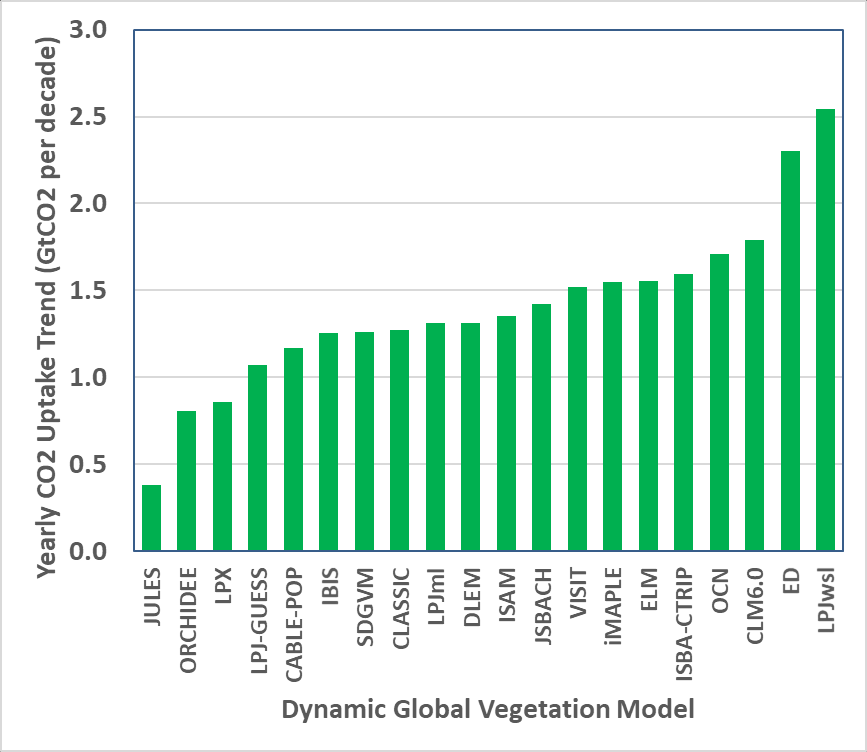
\includegraphics[width=1.0\textwidth]{bilder/bilderKlima-0013.png}\\[1cm]
\end{center}
\caption{Trends der jährlichen CO2-Aufnahme (GtCO2 pro Jahr und Jahrzehnt) durch Landprozesse
im Zeitraum 1959–2023, simuliert durch 20 verschiedene dynamische globale Vegetationsmodelle, die regelmäßig
vom Global Carbon Project (Friedlingstein, 2024) veröffentlicht werden.}
\end{figure}

\subsubsection*{CO$_2$-Aufnahme durch Landprozesse}
Die Aufnahme von zusätzlichem CO$_2$ aus der Atmosphäre durch Landoberflächenprozesse (wie auch aus der globalen Ergrünung geschlossen) wurde mit 20 verschiedenen dynamischen globalen Vegetationsmodellen modelliert, deren Ausgaben jährlich vom Global Carbon Project aktualisiert werden (Friedlingstein, 2024). Wie in Abb. 3.2.3 zu sehen ist, stimmen alle diese Modelle darin überein, dass Vegetation und Böden Kohlenstoff aus der Atmosphäre sequestriert haben. Aber wir sehen auch, dass die langfristigen Trends über 1959 bis 2023 (65 Jahre) stark zwischen den Modellen variieren, um fast einen Faktor von 7. Dies zeigt, dass erhebliche Unsicherheit darüber besteht, wie schnell Landprozesse CO$_2$ aus der Atmosphäre entfernen, was wiederum Unsicherheit in zukünftigen atmosphärischen CO$_2$-Konzentrationen schafft, die dann Unsicherheit in Klimamodellsimulationen zukünftiger Klimaveränderungen erzeugen.

\subsubsection*{CO$_2$-Aufnahme durch Ozeanprozesse}
Die Aufnahme von zusätzlichem CO$_2$ aus der Atmosphäre durch Ozeanprozesse wurde mit 10 verschiedenen Ozeanbiogeochemie-Modellen modelliert, deren Ausgaben jährlich vom Global Carbon Project aktualisiert werden (Friedlingstein, 2024). Wie die Ergebnisse der Landmodelle stimmen alle Ozeanmodelle darin überein, dass die globalen Ozeane während 1959-2023 Kohlenstoff aus der Atmosphäre mit einer steigenden Rate sequestriert haben (Abb. 3.2.4). Im Gegensatz zu den Landmodellen zeigen die Ozeanmodelle jedoch eine viel bessere Übereinstimmung miteinander, wobei das Modell mit der schnellsten steigenden CO$_2$-Aufnahme nur 65 Prozent schneller ist als das Modell mit der langsamsten steigenden CO$_2$-Aufnahme. Trotz der relativen Übereinstimmung zwischen den Modellen bemerkt Friedlingstein et al. (2022), dass es erhebliche Diskrepanzen zwischen den verschiedenen Methoden über die Stärke der Ozeansenke im letzten Jahrzehnt gibt, besonders im Südozean.
Beachten Sie, dass der durchschnittliche Trend in der CO$_2$-Aufnahme über alle Landmodelle in Abb. 3.2.3 25 Prozent größer ist als der durchschnittliche Trend in der Ozeanaufnahme. Dies deutet darauf hin, dass Landprozesse in ihrer Fähigkeit, CO$_2$ zu entfernen, schneller zunehmen als Ozeanprozesse ihre CO$_2$-Sequestrierung steigern.

\begin{figure}[H]
\begin{center}
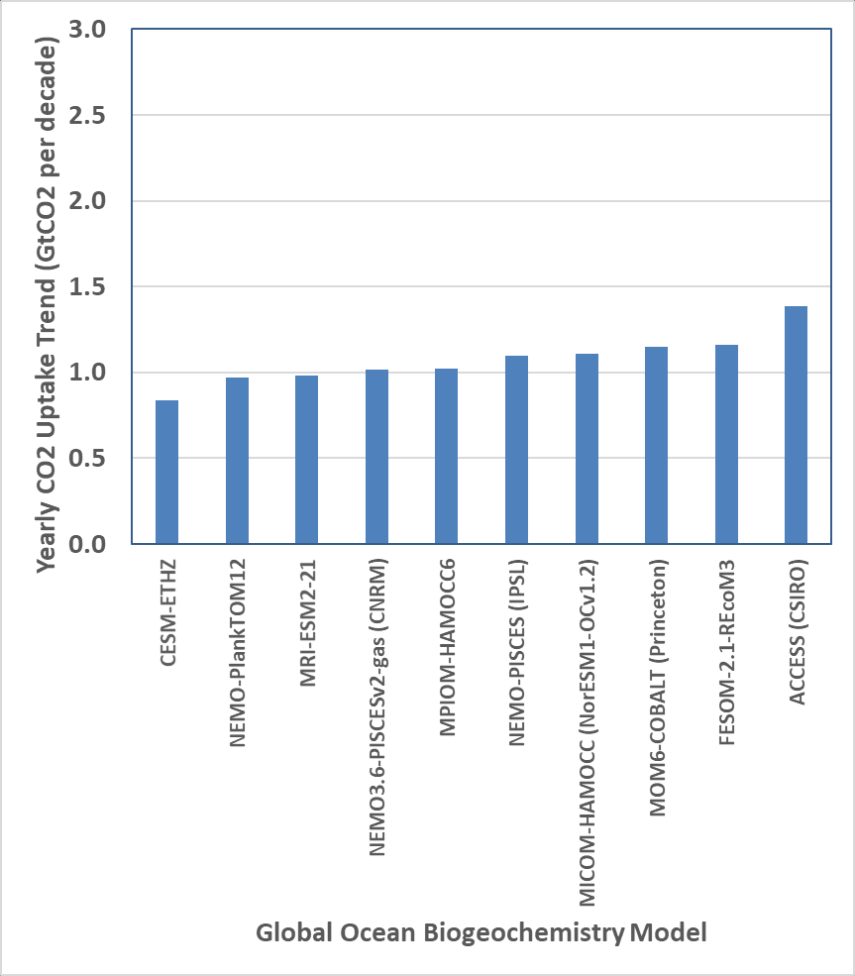
\includegraphics[width=1.0\textwidth]{bilder/bilderKlima-0015.png}\\[1cm]
\end{center}
\caption{Trends der jährlichen CO2-Aufnahme (GtCO2 pro Jahr und Jahrzehnt) durch Ozeanprozesse im Zeitraum
1959–2023, simuliert durch 10 verschiedene ozeanische Biogeochemie-Modelle, regelmäßig berichtet vom
Global Carbon Project (Friedlingstein, 2024).}
\end{figure}


\section{Urbanisierungseinfluss auf Temperaturtrends}
Historische Temperaturdaten über Land wurden hauptsächlich dort gesammelt, wo Menschen leben. Dies wirft das Problem auf, wie man nicht-klimatische Erwärmungssignale aufgrund von städtischen Wärmeinseln (UHI) und anderen Veränderungen der Landoberfläche herausfiltern kann. Wenn diese nicht entfernt werden, könnten die Daten beobachtete Erwärmung übermäßig Treibhausgasen zuschreiben. Das IPCC erkennt an, dass Rohtemperaturdaten mit UHI-Effekten kontaminiert sind, behauptet aber, Datenbereinigungsverfahren zu haben, die sie entfernen. Es ist eine offene Frage, ob diese Verfahren ausreichend sind.
AR6 spielte dieses Problem herunter, indem es sagte (WGI S. 235), dass keine neuen Beweise aufgetaucht seien, um die AR5-Feststellung zu ändern, dass Urbanisierung eine Aufwärtsverzerrung von nicht mehr als 10 Prozent im globalen Landerwärmungstrend verursacht. AR5 (WGI S. 189) zitierte ebenfalls die 10-Prozent-Obergrenze ohne Quellenangabe. AR4 (WGI S. 244) zitierte Jones et al. (1990) und Peterson et al. (1999) als Grundlage der Behauptung. Peterson et al. fanden keinen Unterschied in Trends zwischen ländlichen und städtischen Stichproben, obwohl ihre Definition von ländlich lokale Bevölkerungen bis zu 10.000 Personen einschloss, während der relative Einfluss der Urbanisierung deutlich darunter beginnt (Spencer et al., 2025). Jones et al. verglichen ländliche/städtische Erwärmung in drei Regionen: Ostaustralien, Ostchina und Westliche Sowjetunion. Ihre Definition von \emph{ländlich} umfasste Städte bis zu 10.000 in der ehemaligen Sowjetunion und bis zu 100.000 in China. Sie fanden relative Erwärmungsverzerrungen größer als 10 Prozent in diesen Gebieten, vermuteten aber, dass der Urbanisierungseffekt, gemittelt über die Gebiete, die sie nicht untersuchten, die globale Landverzerrung auf unter 10 Prozent des beobachteten Erwärmungstrends bringen würde.

Mehrere Arbeiten erschienen vor dem IPCC AR4, die argumentierten, dass der erwärmende Effekt von UHIs eine relativ große (30-50\%) Komponente zur beobachteten Erwärmung hinzufügte und nicht von Klimamodellen simuliert wurde (de Laat und Maurellis 2006, McKitrick und Michaels 2007). Diese Befunde basierten auf Korrelationen zwischen Orten maximaler Erwärmung über Land und Orten maximaler sozioökonomischer Entwicklung. AR4 behauptete (S. 244), dass diese Korrelationen ein Artefakt natürlicher atmosphärischer Zirkulationen waren und tatsächlich statistisch insignifikant, und verwarf die Befunde auf dieser Grundlage. Ihre Behauptung war kontrovers, weil sie ohne unterstützende Beweise präsentiert wurde. McKitrick (2010) und McKitrick und Nierenberg (2010) zeigten, dass die Berücksichtigung verschiedener vermuteter alternativer Erklärungen für die Korrelationen ihre Signifikanz nicht beeinflusste. AR5 (S. 189) räumte ein, dass AR4 \emph{keine expliziten Beweise} für seine Bewertung geliefert hatte und erkannte weiter auf der Grundlage dieser Arbeiten an, dass es \emph{signifikante Beweise für eine solche Kontamination der Aufzeichnung} gab, d.h. eine Erwärmungsverzerrung in der Landaufzeichnung. Wie bereits bemerkt, trugen sie jedoch an anderer Stelle im AR5-Bericht die AR4-Behauptung vor, dass es weniger als 10 Prozent der beobachteten Erwärmung seien. Außerdem gaben sie keine Warnung über die Verwendung der Landaufzeichnung für Klimamessungen, obwohl sie die Beweise für UHI-Kontamination einräumten. Kürzlich schätzten Soon et al. (2023) eine Urbanisierungsverzerrung in der nordhemisphärischen Landaufzeichnung über 1850-2018, die ausreicht, um den Trend in der gemischten Aufzeichnung von \SI{0.55}{\celsius} auf \SI{0.89}{\celsius} pro Jahrhundert zu erhöhen.

Einige Studien, die Beweise gegen UHI-Kontamination lieferten, verglichen Erwärmungsraten zwischen ländlichen und städtischen Standorten (Jones et al. 1990, Peterson et al. 1999, Wickham et al. 2013). Es ist nicht bekannt, ob solche Methoden UHI-Verzerrung erkennen könnten, selbst wenn sie vorhanden wäre. Der Einfluss der UHI-Erwärmung ist logarithmisch in der Bevölkerung, mit anderen Worten, er ist am stärksten bei niedriger Bevölkerungsdichte und flacht dann ab, wenn sich die lokale Urbanisierung ausdehnt (Oke 1973, Spencer et al. 2025). Daher beweist das Versagen, einen Unterschied in Erwärmungsraten zwischen städtischen und ländlichen Stationen zu finden, nicht die Abwesenheit von UHI-Kontamination. McKitrick (2013) lieferte eine empirische Demonstration, in der sich die ländlichen/städtischen Trends in einem Datensatz, der aus anderen Gründen als mit UHI-Verzerrung kontaminiert erwiesen wurde, nicht signifikant unterschieden.

Parker (2006) untersuchte eine Stichprobe städtischer Standorte und fand keinen Unterschied in Trends zwischen Untergruppen, die nach nächtlicher Windgeschwindigkeit unterteilt waren, und schloss auf dieser Grundlage, dass Urbanisierung kein signifikanter Faktor sein könnte. Auch hier ist die Frage, ob eine solche Methode UHI-Verzerrung finden würde, selbst wenn sie vorhanden wäre. McKitrick (2013) präsentierte ein Beispiel, in dem UHI-kontaminierte Daten keine signifikanten Trendunterschiede zeigten, wenn sie nach Windgeschwindigkeit stratifiziert wurden.

Die Herausforderung bei der Messung von UHI-Verzerrung besteht darin, lokale Temperaturveränderungen mit einer entsprechenden Veränderung in Bevölkerung oder Urbanisierung zu verknüpfen, anstatt mit einer statischen Klassifikationsvariable wie ländlich oder städtisch. Spencer et al. (2025) verwendeten neu verfügbare historische Bevölkerungsarchive, um eine solche Analyse durchzuführen, und fanden Beweise für signifikante UHI-Verzerrung in US-Sommertemperaturdaten.

Zusammenfassend, während es eindeutig Erwärmung in der Landaufzeichnung gibt, gibt es auch Beweise dafür, dass sie durch Urbanisierungsmuster nach oben verzerrt ist und dass diese Verzerrungen nicht vollständig durch die Datenverarbeitungsalgorithmen entfernt wurden, die zur Erstellung von Klimadatensätzen verwendet werden.

\vfill
\noindent\textbf{Literaturverzeichnis:}

\begingroup
\parindent=0pt
\everypar{\hangindent=2em\hangafter=1\relax}

Angert, A., S. Biraud, Bonfils, C., Buermann, W. and I. Fung (2004). CO2 seasonality indicates origins of
post-Pinatubo sink. Geophysical Research Letters 31. \url{https://doi.org/10.1029/2004GL019760}

AR6: Intergovernmental Panel on Climate Change Sixth Assessment Report (2021) Working Group I
Contribution. www.ipcc.ch.

AR5: Intergovernmental Panel on Climate Change Fifth Assessment Report (2013) Working Group I
Contribution. www.ipcc.ch.

AR4: Intergovernmental Panel on Climate Change Fourth Assessment Report (2007) Working Group I
Contribution. www.ipcc.ch.

Burgess, Matthew et al (2021) Environmental Research Letters 16 014016
\url{https://iopscience.iop.org/article/10.1088/1748-9326/abcdd2/meta}

Ciais, P., C. Sabine, G. Bala, L. Bopp, V. Brovkin,et al. (2013): Carbon and Other Biogeochemical Cycles.
In: Climate Change 2013: The Physical Science Basis. Contribution of Working Group I to the Fifth
Assessment Report of the Intergovernmental Panel on Climate Change [Stocker, T.F., D. Qin, G.-K.
Plattner, M. Tignor,et al. (eds.)]. Cambridge University Press, Cambridge, United Kingdom and New
York, NY, USA

Connolly, Roman, Willie Soon, Michael Connolly et al. (2021) How much has the Sun influenced
Northern Hemisphere temperature trends? An ongoing debate Research in Astronomy and
Astrophysics 21(6) doi: 10.1088/1674-4527/21/6/131 \url{https://iopscience.iop.org/article/10.1088/1674-
4527/21/6/131}

Crisp, David \& Dolman, Han (A.J.) \& Tanhua, Toste \& Mckinley, Galen \& Hauck, Judith \& Bastos, Ana
\& Sitch, Stephen \& Eggleston, Simon \& Aich, Valentin. (2022). How Well Do We Understand the
Land‐Ocean‐Atmosphere Carbon Cycle?. Reviews of Geophysics. 60. 10.1029/2021RG000736.

De Laat, A.T.J., and A.N. Maurellis (2006), Evidence for influence of anthropogenic surface processes on
lower tropospheric and surface temperature trends, International Journal of Climatology 26:897—913.

Friedlingstein, P., and 95 co-authors (2024): Global Carbon Budget 2024, Earth System Science Data
14(4), https://essd.copernicus.org/preprints/essd-2024-519

Hausfather et al. (2019) “Evaluating the Performance of Past Climate Model Projections” Geophysical
Research Letters 47(1) https://doi.org/10.1029/2019GL085378

Hausfather, Z. and G. Peters (2020a) “Emissions – the ‘business as usual’ story is misleading” Nature 29
January 2020 https://www.nature.com/articles/d41586-020-00177-3

Hausfather, Z. and G. Peters (2020b) RCP8.5 is a problematic scenario for near-term emissions.
Proceedings of the National. Academy of Sciences 117, 27791–27792 (2020)

Jenkins, S., Smith, C., Allen, M. et al. Tonga eruption increases chance of temporary surface temperature
anomaly above 1.5 °C. Nature Climate Change. 13, 127–129 (2023). https://doi.org/10.1038/s41558-
022-01568-2

Jones, P. D., P. Y. Groisman, M. Coughlan, N. Plummer, W.-C. Wang, and T. R. Karl (1990),
Assessment of urbanization effects in time series of surface air temperature over land, Nature, 347,
169 – 172

Liu, Pengfei et al. (2021) “Improved estimates of preindustrial biomass burning reduce the magnitude of
aerosol climate forcing in the Southern Hemisphere” Science Advances 7(22) May 2021
https://doi.org/10.1126/sciadv.abc1379

McKitrick, R.R. and P.J. Michaels (2007), Quantifying the influence of anthropogenic surface processes
and inhomogeneities on gridded global climate data, Journal of Geophysical Research, 112, D24S09,
doi:10.1029/2007JD008465.

McKitrick, Ross R. (2010) Atmospheric Oscillations Do Not Explain the Temperature-Industrialization
Correlation. Statistics Politics and Policy Vol 1. No. 1., July 2010

McKitrick, Ross R. (2013) Encompassing Tests of Socioeconomic Signals in Surface Climate
Data. Climatic Change doi 10.1007/s10584-013-0793-5. Volume 120, Issue 1-2.
http://link.springer.com/article/10.1007%2Fs10584-013-0793-5

McKitrick, Ross R. and Nicolas Nierenberg (2010) Socioeconomic Patterns in Climate Data. Journal of
Economic and Social Measurement, 35(3,4) pp. 149-175. DOI 10.3233/JEM-2010-0336

McKitrick, Ross R., Mark Strazicich and Junsoo Lee (2012) “Long-Term Forecasting of Global Carbon
Dioxide Emissions: Reducing Uncertainties Using a Per-Capita Approach.” Journal of
Forecasting, Vol 32, Issue 5, pp 435-451 DOI: 10.1002/for.2248.

Oke, T.R., 1973: City size and the urban heat island, Atmospheric Environment 7, 769-779

Parker, D.E. (2006) “A Demonstration that Large-Scale Warming is not Urban.” Journal of Climate
19:2882—2895.

Peterson, Thomas C., Kevin P. Gallo, Jay Lawrimore, Timothy W. Owen, Alex Huang, David A.
McKittrick (1999) Global rural temperature trends. Geophysical Research Letters February 1999
https://doi.org/10.1029/1998GL900322

Pielke Jr., Roger and Ritchie, Justin (2020) “Systemic Misuse of Scenarios in Climate Research and
Assessment” Social Sciences Research Network April 2020, available at:
https://ssrn.com/abstract=3581777

Pielke Jr, R., Burgess, M. G., \& Ritchie, J. (2022). Plausible 2005-2050 emissions scenarios project
between 2 and 3 degrees C of warming by 2100. Environmental Research Letters 17 024027
https://iopscience.iop.org/article/10.1088/1748-9326/ac4ebf/pdf

Scaffeta, Nicola, Richard C. Willson, Jae N. Lee and Dong Wu (2019) Modeling Quiet Solar Luminosity
Variability from TSI Satellite Measurements and Proxy Models during 1980–2018. Remote Sensing
11(21) 2569 https://doi.org/10.3390/rs11212569

Schoeberl, M.R., Y. Wang, G. Taha, D.J. Zawada, R. Ueyama and A. Dessler, 2024. Evolution of the
climate forcing during the two years after the Hunga Tonga-Hunga Ha’apai eruption. Journal of
Geophysical Research., 129.

Schwalm, C.R., S. Glendon, P. B. Duffy (2020) RCP8.5 tracks cumulative CO2 emissions. Proceedings of
the National Academy of Sciences U.S.A. 117, 19656–19657 (2020).

Soon,W.; Connolly, R.; Connolly, M.; Akasofu, S.-I.; Baliunas, S.; et al. (2023) The Detection and
Attribution of Northern Hemisphere Land Surface Warming (1850–2018) in Terms of Human and
Natural Factors: Challenges of Inadequate Data. Climate 2023, 11, 179.
https://doi.org/10.3390/cli11090179

Spencer, Roy W, John R Christy and William D. Braswell (2025) Urban Heat Island Effects in U.S.
Summer Surface Temperature Data, 1895–2023 Journal of Applied Meteorology and Climatology
April 2025 https://doi.org/10.1175/JAMC-D-23-0199.1

Wickham C, R Rohde , RA Muller, J Wurtele, J Curry, et al. (2013) Influence of Urban Heating on the
Global Temperature Land Average using Rural Sites Identified from MODIS Classifications.
Geoinformatics and Geostatistics: An Overview 1:2.

Zacharias, Pia (2014) An Independent Review of Existing Total Solar Irradiance Records. Surveys in
Geophysics 35 pp. 897—912 https://link.springer.com/article/10.1007/s10712-014-9294-y
\endgroup

\cleardoublepage
\chapter*{TEIL II: KLIMAREAKTION AUF CO$_2$-EMISSIONEN}
%\numberwithin{figure}{chapter}
\FigureNumbersByChapter
\addcontentsline{toc}{chapter}{TEIL II: KLIMAREAKTION AUF CO$_2$-EMISSIONEN}
\cleardoublepage
\chapter{Klimasensitivität bezüglich CO$_2$-Einwirkung}
\paragraph{Kapitelzusammenfassung}
\begin{quote}
Es gibt eine wachsende Erkenntnis, dass Klimamodelle nicht für den Zweck geeignet sind, die Gleichgewichts-Klimasensitivität (ECS) des Klimas gegenüber steigendem CO$_2$ zu bestimmen. Das IPCC hat sich datengetriebenen Ansätzen zugewandt, einschließlich historischer Daten und paläoklimatischer Rekonstruktionen, aber deren Zuverlässigkeit ist durch Datenmängel beeinträchtigt.
Datengetriebene ECS-Schätzungen tendieren dazu, niedriger zu sein als klimamodell-generierte Werte. Die obere Grenze des IPCC AR6 für den wahrscheinlichen ECS-Bereich beträgt \SI{4.0}{\celsius}, niedriger als der AR5-Wert von \SI{4.5}{\celsius}. Diese Senkung der oberen Grenze scheint durch paläoklimatische Daten gut begründet zu sein. Die untere Grenze des AR6 für den wahrscheinlichen ECS-Bereich beträgt \SI{2.5}{\celsius}, wesentlich höher als der AR5-Wert von \SI{1.5}{\celsius}. Diese Erhöhung der unteren Grenze ist weniger gerechtfertigt; Belege seit AR6 zeigen, dass die untere Grenze des wahrscheinlichen Bereichs bei etwa \SI{1.8}{\celsius} liegt.
\end{quote}
\section{Einleitung}
Das Ausmaß der Klimareaktion auf steigende CO$_2$-Konzentrationen steht im Zentrum der wissenschaftlichen Debatte über den anthropogenen Klimawandel und damit auch der öffentlichen Debatte über \emph{Klimaschutzmaßnahmen}. Das einfachste Maß für diese Reaktion ist der Anstieg der globalen durchschnittlichen Oberflächentemperatur, quantifiziert durch die Gleichgewichts-Klimasensitivität (ECS). ECS ist definiert als das Ausmaß der Erwärmung, das als Reaktion auf eine Verdoppelung von CO$_2$ von seiner vorindustriellen Konzentration von \SI{280}{ppm} erwartet wird, nachdem alle Klimakomponenten Zeit hatten, sich anzupassen. Einige Komponenten, wie die Temperaturen in der unteren Atmosphäre (Troposphäre), passen sich schnell an, während andere wie der tiefe Ozean und die Kryosphäre möglicherweise jahrhundertelang brauchen. Ein verwandtes Maß, die Transiente Klimareaktion (TCR), beschreibt die kürzeren Zeitskalen besser; sie ist definiert als das Ausmaß der Erwärmung, wenn die CO$_2$-Konzentration durch einen jährlichen Anstieg von einem Prozent über 70 Jahre verdoppelt wird.

Der Charney-Bericht von 1979 für die U.S. National Academy of Sciences (National Research Council 1979) schlug vor, dass die wahrscheinlichste ECS \SI{3.0}{\celsius} $\pm$ \SI{1.5}{\celsius} sei. Das IPCC bekräftigte diesen Bereich wiederholt mit nur geringfügigen Variationen bis zu seinem jüngsten AR6. AR5 bezeichnete \SIrange{1.5}{4.5}{\celsius} als den wahrscheinlichen Bereich (66 Prozent Wahrscheinlichkeit) und stellte fest, dass ECS extrem unwahrscheinlich (95 Prozent Wahrscheinlichkeit) unter \SI{1.0}{\celsius} und sehr unwahrscheinlich (90 Prozent Wahrscheinlichkeit) über \SI{6.5}{\celsius} liegt.

Die Unsicherheit in ECS ist hartnäckig weit geblieben, trotz vieler einzelner Studien, die behaupteten, sie zu verringern (Hausfather 2023). Zuletzt verengte AR6 den wahrscheinlichen Bereich auf \SIrange{2.5}{4.0}{\celsius} und betrachtete den sehr wahrscheinlichen Bereich als \SIrange{2.0}{5.0}{\celsius}. Diese Verengung am unteren Ende wird bestritten, wie unten diskutiert wird.

Unsicherheiten in ECS sind höchst folgenreich für die Politikgestaltung. Wie in Kapitel 11 diskutiert wird, verwenden Wirtschaftsmodelle ECS-Werte, um die Kosten von CO$_2$-Emissionen zu projizieren. Der traditionelle Wert (\SI{3.0}{\celsius}) hat typischerweise bescheidene globale soziale Kosten von CO$_2$-Emissionen ergeben, ausreichend um einige politische Maßnahmen zu rechtfertigen, aber meist auf später in diesem Jahrhundert verschoben. Wenn ECS sehr hoch ist (über \SI{4.5}{\celsius}), werden sofortige aggressive Emissionskontrollen zwingender, während keine CO$_2$-Emissionskontrollen wirtschaftlich gerechtfertigt sind für ECS unter \SI{2.0}{\celsius} (Dayaratna et al. 2017, 2020). Eine präzise Schätzung zu erhalten ist unmöglich, daher muss die Politikgestaltung die Unsicherheit berücksichtigen.

Für sich allein ist der Gleichgewichts-Erwärmungseffekt einer Verdoppelung des atmosphärischen CO$_2$ etwas mehr als \SI{1}{\celsius} (Soden und Held 2006). Größere Werte von ECS entstehen durch positive Rückkopplungen, die die CO$_2$-Erwärmung verstärken. Wasserdampf-Rückkopplung ist positiv: eine wärmere Atmosphäre könnte mehr Wasserdampf haben, der selbst ein starkes Treibhausgas ist. Wärmere Temperaturen führen auch zu weniger Schnee- und Meereisbedeckung, wodurch die Erde mehr von der Sonnenstrahlung absorbieren kann. Einige einfache Schätzungen dieser Rückkopplungen erhöhen die ECS auf etwa \SI{2}{\celsius} (Sherwood et al., 2020). Größere Werte von ECS sind mit positiven Wolken-Rückkopplungen verbunden.

Klimawissenschaftler verwenden mehrere Beweislinien, um die Gleichgewichts-Klima\-sensitivität zu bestimmen:
\begin{itemize}
\item  Klimamodell-Simulationen
\item  Historische Beobachtungen  
\item  Paläoklimatische Rekonstruktionen
\item  Prozessverständnis von Rückkopplungen
\end{itemize}

\section{Modellbasierte Schätzungen der Klimasensitivität}
Die in IPCC AR4 und AR5 angegebenen ECS-Bereiche wurden hauptsächlich durch die Untersuchung des Verhaltens großmaßstäblicher Klimamodelle, auch General Circulation Models (GCMs) genannt, erhalten. Das IPCC änderte jedoch den Kurs in seinem AR6, als es sich einer direkteren datengetriebenen Methodik zuwandte. Hier diskutieren wir einige der Fallstricke bei der Verwendung von GCMs, um die Klimasensitivität der Erde zu bestimmen.

ECS kann aus Klimamodell-Simulationen bestimmt werden, indem die CO$_2$-Konzentration verdoppelt und mehrere Jahrhunderte für die Erwärmung zum Gleichgewicht ermöglicht werden. Um die Notwendigkeit solch langer Simulationen zu vermeiden, wird \emph{effektive Klimasensitivität} üblicherweise aus einer 150-Jahres-Simulation als Reaktion auf eine plötzliche Vervierfachung von CO$_2$ bewertet.

Im Prinzip ist ECS eine emergente Eigenschaft von GCMs –- das heißt, sie wird nicht direkt parametrisiert oder abgestimmt, sondern entsteht vielmehr in den Ergebnissen der Simulation. Anderweitig plausible GCMs und Parameterauswahlen wurden verworfen wegen wahrgenommener Konflikte mit einer erwarteten Erwärmungsrate oder Abneigung gegen eine Klimasensitivität des Modells außerhalb eines akzeptierten Bereichs (Mauritsen et al. 2012). Diese Praxis war für die in AR4 verwendeten Modelle üblich; Modellierer sind mit der Zeit von dieser Praxis abgekommen. Jedoch, selbst in einem CMIP6-Modell, stellen Mauritsen und Roeckner (2020) das Folgende bezüglich ihres Max-Planck-Institut (MPI) Klimamodells fest (Hervorhebung hinzugefügt):

\begin{quote}
Wir haben dokumentiert, wie wir das globale Klimamodell MPI-ESM1.2 abstimmten, um der instrumentellen Aufzeichnung der Erwärmung zu entsprechen; ein Unterfangen, das eindeutig erfolgreich war. Aufgrund der historischen Reihenfolge der Ereignisse war die Wahl, dies praktisch zu tun, indem eine ECS von etwa 3 K mittels Wolken-Rückkopplungen anvisiert wurde, anstatt die Aerosol-Forcierung abzustimmen.  
\end{quote}

Mit anderen Worten, die MPI-Modellierer wählten einen ECS-Wert von \SI{3}{\celsius} und stimmten dann die Wolken-Parametrisierungen ab, um ihr beabsichtigtes Ergebnis zu erreichen.

Wie bemerkt, ist die direkte Erwärmung durch CO$_2$-Verdoppelung nur etwa \SI{1}{\celsius} (Soden und Held 2006); weitere Erwärmung entsteht durch Klima-Rückkopplungen, die nicht explizit vom GCM aufgelöst werden, sondern auf Parametrisierungen physikalischer Prozesse angewiesen sind. Höhere Werte von ECS entstehen primär durch positive Wolken-Rückkopplungen, während das Ausmaß und sogar das Vorzeichen der Rückkopplungen sehr unsicher sind. Elemente der Wolken-Rückkopplung umfassen Änderungen in der Breitenverteilung von Wolken, Änderungen in der Verteilung der Wolkenhöhe (Änderungen in niedrigen versus hohen Wolken), Änderungen in der Phase von Wolken (Eis versus Flüssigkeit), Änderungen in der Wolkenpartikelgröße (verbunden mit Änderungen in Konzentration und/oder Zusammensetzung von Aerosolpartikeln), Änderungen in der Niederschlagseffizienz von Wolken, und sogar Änderungen darin, wie Wolken über den täglichen Sonnenzyklus verteilt sind (Curry und Webster, 1999). Es ist für GCMs schwierig, irgendeinen dieser Prozesse aufgrund ihrer kleinen Skala korrekt zu simulieren, geschweige denn vorherzusagen, wie sie sich in der Zukunft ändern werden. Weiterhin modulieren Wolkenprozesse die Größenordnungen der Wasserdampf-, Lapse-Rate- und Oberflächenalbedo-Rückkopplungen.

\begin{figure}[H]
\begin{center}
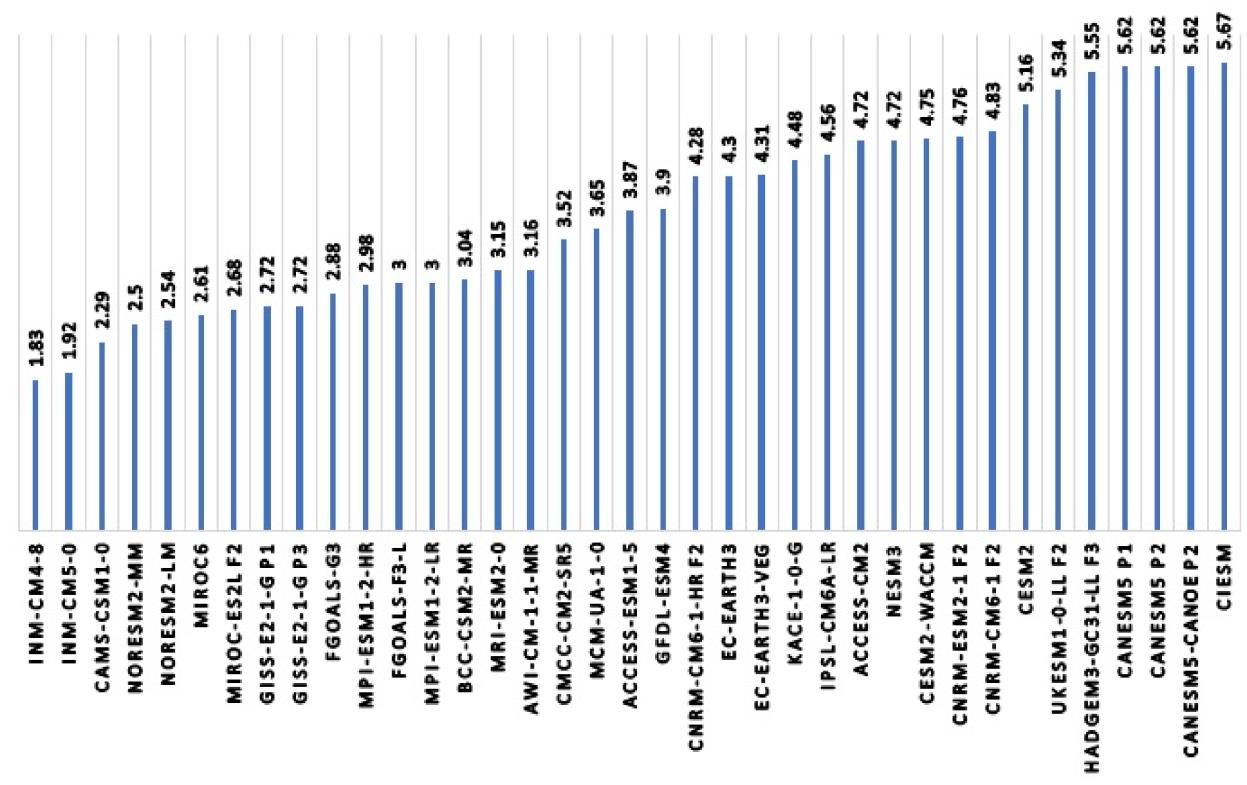
\includegraphics[width=1.0\textwidth]{bilder/bilderKlima-0017.jpg}\\[1cm]
\end{center}
\caption{Gleichgewichtsklimasensitivitäten in °C von 37 Klimamodellen aus dem CMIP6-Ensemble.
Die Kennungen für die verschiedenen Modelle sind auf der horizontalen Achse angegeben. Aus (Scafetta, 2021)}
\end{figure}


Die Spannweite der ECS-Werte aus dem CMIP5-Ensemble von Klimamodellen, die in AR5 verwendet wurden, war \SIrange{2.0}{4.7}{\celsius}; dieser Bereich vergrößerte sich für die CMIP6-Modelle, die in AR6 verwendet wurden, auf zwischen $1.8$ und \SI{5.7}{\celsius} (Chen et al., 2021, Scaffeta 2021, siehe Abbildung 4.1). Weit davon entfernt, die modellbasierte Klimasensitivität aufzulösen, scheint sich der Bereich zu vergrößern. Die Hauptursache der gesamten Aufwärtsverschiebung in ECS in CMIP6 relativ zu CMIP5 ist eine größere positive Wolken-Rückkopplung, angetrieben durch Änderungen in den Wolken-Parametrisierungen in vielen CMIP6-Modellen (Zelinka et al., 2020).

Aufgrund von Bedenken über Modellabstimmung und die hohe Empfindlichkeit gegenüber Wolken-Parametrisierungen stützte sich AR6 (2021) nicht auf Klimamodell-Simulationen in ihrer Bewertung der Klimasensitivität, sondern verließ sich stattdessen auf datengetriebene Methoden.

\section{Datengetriebene Schätzungen der Klimasensitivität}
Klimasensitivität kann auch aus instrumentellen Aufzeichnungen von Oberflächentemperaturen und ozeanischem Wärmeinhalt geschätzt werden, kombiniert mit Schätzungen darüber, wie sich Klimaforcierungen (z.B. Treibhausgase, solar, Vulkane, Aerosole) in der Vergangenheit verändert haben (Otto et al., 2013). Mit dieser Information kann ein einfaches empirisches Energiebilanz-Modell eingesetzt werden. Es erfordert die Schätzung eines Rückkopplungsparameters, dessen Unsicherheiten in der resultierenden ECS stark verstärkt werden (Roe und Baker, 2007).

Die Genauigkeit der datengetriebenen Methoden hängt von der Qualität der Eingangsdaten ab. Annahmen sind über ozeanische Wärmespeicherung nötig, und gute Daten sind nur für die letzten Jahrzehnte verfügbar. Die größte Quelle der Unsicherheit ist die Menge und Zusammensetzung von Aerosolpartikeln und ihre Wechselwirkungen mit Wolkenstrahlungseigenschaften (der sogenannte indirekte Aerosoleffekt; siehe Abbildungen 3.1.1, 3.1.2). Klimamodelle zeigen Erwärmung als Reaktion auf THG, aber Abkühlung als Reaktion auf Aerosole (Schwartz et al., 2007). Beobachtete Erwärmung des 20. Jahrhunderts kann gezeigt werden, dass sie konsistent ist entweder mit niedriger ECS und niedriger Aerosol-Abkühlung, oder hoher ECS und hoher Aerosol-Abkühlung. Da die Verwendung fossiler Brennstoffe sowohl THG als auch Aerosole zur Atmosphäre hinzufügt, müssen beide Effekte geschätzt werden, um den Erwärmungseffekt von CO$_2$ zu isolieren.

Paläoklima-Proxies werden auch verwendet, um die Sensitivität vergangener Klimate zu bewerten, indem paläoklimatische Änderungen in den Erdtemperaturen mit Schätzungen von Änderungen in Forcierungen verglichen werden. Die zwei informativsten Perioden sind das letzte glaziale Maximum (vor etwa 20.000 Jahren), das etwa \SIrange{3}{7}{\celsius} kälter war als heute, und eine mittlere Pliozän-Periode (vor etwa drei Millionen Jahren), die \SIrange{1}{3}{\celsius} wärmer war als heute. Die Grenzen der Abkühlung während des letzten glazialen Maximums geben den besten einzelnen Beweis, dass hohe Werte der Klimasensitivität unwahrscheinlich sind. Jedoch sind paläoklimatische Schätzungen mit sehr großen Unsicherheiten in den geschätzten Temperaturen und Forcierungen verbunden. Weiterhin könnten Schätzungen der Klimasensitivität basierend auf vergangenen Klimazuständen nicht auf den aktuellen Zustand des Klimasystems anwendbar sein.

Ein wiederkehrendes Thema in der Klimaliteratur ist, dass ECS-Schätzungen basierend auf historischen Daten kleiner sind als ECS-Schätzungen, die aus Klimamodellen abgeleitet werden (Sherwood und Forest 2024). Etwa 15 Schätzungen basierend auf historischen Daten erschienen in der begutachteten Literatur zwischen 2012 und 2024, die ECS-Bestschätzungen zwischen \SI{1.0}{\celsius} und \SI{2.5}{\celsius} ergaben, obwohl Kritiker einige der Methoden und die Datenqualität in Frage gestellt haben. Für AR6 legte das IPCC primäres Gewicht auf die Ergebnisse von Sherwood et al. (2020), die historische Daten und paläoklimatische Proxies mit dem prozessbasierten Ansatz kombinierten und eine Bestschätzung von \SI{3.1}{\celsius} mit einem wahrscheinlichen Bereich von \SIrange{2.6}{3.9}{\celsius} ergaben. Lewis (2022) äußerte eine Reihe von Bedenken über dieses Ergebnis, einschließlich methodologischer Fehler, veralteter Eingangswerte und der Verwendung subjektiver Bayesscher Priors in der Analyse. Lewis' Analyse fand, dass Klimasensitivität geschätzt wird, viel niedriger und besser eingegrenzt zu sein als in der Sherwood et al. Analyse – Median \SI{2.2}{\celsius} (\SIrange{1.8}{2.7}{\celsius} im $17-83$ Prozent wahrscheinlichen Bereich, und \SIrange{1.6}{3.2}{\celsius} im $5-95$ Prozent sehr wahrscheinlichen Bereich). Das IPCC AR6 schätzte nur eine $5$ Prozent Wahrscheinlichkeit, dass ECS unter \SI{2.3}{\celsius} lag, während Lewis es auf über $50$ Prozent schätzte. Die jüngsten Veröffentlichungen in der Debatte zwischen Sherwood et al. und Lewis verteidigen weiterhin ihre jeweiligen Positionen: Sherwood und Foster (2024) und Lewis (2025).

Ein in AR6 betontes Argument ist, dass datengetriebene ECS-Schätzungen die zukünftige Erwärmungsreaktion auf THG unterschätzen könnten wegen eines sogenannten \emph{Mustereffekts} (Forster et al., 2021). Es wird geglaubt, dass der tropische Pazifik die Gesamteffizienz, mit der die Erde Wärme in den Weltraum abstrahlt, stark beeinflusst, aber einige Regionen entfernen Wärme effizienter als andere. Wenn der West-Ost-Temperaturgradient im tropischen Pazifik in einem sich erwärmenden Klima geschwächt wird, würde sich die Erwärmung dort konzentrieren, wo Wärme weniger effizient entfernt wird, was ECS erhöht.

Die meisten Klimamodelle simulieren, dass steigende THG den West-Ost-Temperatur\-gradienten schwächen werden, was das IPCC in AR6 zu dem Schluss führte, dass datengetriebene ECS-Schätzungen den zukünftigen ECS-Wert unterschätzten. Jedoch wiesen Seager et al. (2019) darauf hin, dass, entgegen den Modellen, sich der West-Ost-Temperaturgradient über die Zeit verstärkt hat. Sie argumentierten weiter, dass der Mechanismus, der anderes in Klimamodellen vorhersagt, auf einer fehlerhaften Charakterisierung ozeanischer Dynamik basierte und es keinen Grund gibt zu erwarten, dass sich der Gradient schwächt. Ein ähnliches Argument wurde kürzlich von Lee et al. (2024) gemacht, die schlossen, dass \emph{die Trajektorie des beobachteten Trends die Reaktion auf zunehmende THG-Belastung in der Atmosphäre widerspiegelt}; mit anderen Worten, THG-Erwärmung sollte zu einer zukünftigen Verstärkung statt einer Schwächung des Temperaturgradienten führen. Erhöhte Effizienz der atmosphärischen Abkühlung impliziert, wenn überhaupt, dass die zukünftige ECS in einem sich erwärmenden Klima niedriger sein könnte als aktuelle Schätzungen.

\section{Transiente Klimareaktion}
Die Transiente Klimareaktion (TCR) bietet eine nützlichere Beobachtungseinschränkung für die Klimasensitivität. TCR ist der globale Temperaturanstieg, der entsteht, wenn CO$_2$ mit einer jährlichen Rate von 1 Prozent über einen Zeitraum von 70 Jahren erhöht wird (d.h. allmählich verdoppelt). Im Vergleich zur ECS vermeiden beobachtungsbasiert bestimmte Werte von TCR die Probleme von Unsicherheiten in der ozeanischen Wärmeaufnahme und der unscharfen Grenze bei der Definition des Gleichgewichts, die aus einer Reihe von Zeitskalen für die längerfristigen Rückkopplungsprozesse (z.B. Eisschilde) entstehen. TCR ist durch historische Erwärmung besser eingegrenzt als ECS. AR6 beurteilte den sehr wahrscheinlichen Bereich von TCR als \SIrange{1.2}{2.4}{\celsius}. Im Gegensatz zu ECS ist die obere Grenze von TCR enger eingegrenzt. Zum Vergleich: die von Lewis (2023) bestimmten TCR-Werte liegen bei $1.25$ bis \SI{2.0}{\celsius}, was eine viel bessere Übereinstimmung mit AR6-Werten zeigt, als beim Vergleich der ECS-Werte zu sehen war.

\vfill
\noindent\textbf{Literaturverzeichnis:}

\begingroup
\parindent=0pt
\everypar{\hangindent=2em\hangafter=1\relax}

Carbon Brief. (2020, July 22). Explainer: How scientists estimate climate sensitivity.
\url{https://www.carbonbrief.org/explainer-how-scientists-estimate-climate-sensitivity}

Carbon Brief. (2020, July 22). Guest post: Why low-end ‘climate sensitivity’ can now be ruled out.
\url{https://www.carbonbrief.org/guest-post-why-low-end-climate-sensitivity-can-now-be-ruled-out}

Carbon Brief. (2021, August 9). In-depth Q\&A: The IPCC’s sixth assessment report on climate science.
\url{https://www.carbonbrief.org/in-depth-qa-the-ipccs-sixth-assessment-report-on-climate-science}

Chen, D., et al. (2021). Framing, context, and methods. In V. Masson-Delmotte et al. (Eds.), Climate
change 2021: The physical science basis. Contribution of Working Group I to the Sixth Assessment
Report of the Intergovernmental Panel on Climate Change. Cambridge University Press.

Curry, J. A., \& Webster, P. J. (1999). Thermodynamic feedbacks in the climate system. In
Thermodynamics of atmospheres and oceans (pp. 351–385). Academic Press.

Dayaratna, Kevin, Ross McKitrick and David Kreutzer (2017) Empirically-Constrained Climate Sensitivity
and the Social Cost of Carbon. Climate Change Economics April 2017 DOI:
http://dx.doi.org/10.1142/S2010007817500063

Dayaratna, Kevin, Ross McKitrick and Patrick J. Michaels (2020) Climate Sensitivity, Agricultural
Productivity and the Social Cost of Carbon in FUND. Environmental Economics and Policy Studies
https://doi.org/10.1007/s10018-020-00263-w

Forster, P., et al. (2021). The Earth's energy budget, climate feedbacks, and climate sensitivity. In V.
Masson-Delmotte et al. (Eds.), Climate change 2021: The physical science basis. Contribution of
Working Group I to the Sixth Assessment Report of the Intergovernmental Panel on Climate Change.
Cambridge University Press.

Hausfather, Z. (2020, July 22). Explainer: How scientists estimate climate sensitivity. Carbon Brief.
https://www.carbonbrief.org/explainer-how-scientists-estimate-climate-sensitivity

Lan, X., Tans, P., \& Thoning, K. W. (2025). Trends in globally-averaged CO$_2$ determined from NOAA
Global Monitoring Laboratory measurements. NOAA Global Monitoring Laboratory.
https://doi.org/10.15138/9N0H-ZH07

Lee, S., Byrne, M. P., Loikith, P. C., \& O’Dell, C. W. (2024). Zonal contrasts of the tropical Pacific
climate predicted by a global constraint. Climate Dynamics, 62(1–2), 229–246.
https://doi.org/10.1007/s00382-023-06741-7

Lewis, N. (2023). Objectively combining climate sensitivity evidence. Climate Dynamics, 61(9–10),
3155–3163. https://doi.org/10.1007/s00382-022-06398-8

Lewis, N. (2025). Comment on “Can uncertainty in climate sensitivity be narrowed further?” by
Sherwood and Forest (2024). EGUsphere [preprint]. https://doi.org/10.5194/egusphere-2025-1179

Thorsten Mauritsen et al., (2012) “Tuning the Climate of a Global Model,” Journal of Advances in
Modeling Earth Systems 4, no. 3 https://doi. org/10.1029/2012ms000154


Mauritsen, T., \& Roeckner, E. (2020). Tuning the MPI-ESM1.2 global climate model to improve the
match with instrumental record warming by lowering its climate sensitivity. Journal of Advances in
Modeling Earth Systems, 12, e2019MS002037. https://doi.org/10.1029/2019MS002037

Otto, A., Otto, F. E. L., Boucher, O., Church, J., Hegerl, G., Forster, P. M., Gregory, J. M., \& Johnson, G.
C. (2013). Energy budget constraints on climate response. Nature Geoscience, 6(6), 415–416.
https://doi.org/10.1038/ngeo1836

Pachauri, R. K., \& Meyer, L. (Eds.). (2015). Climate change 2014: Synthesis report. Intergovernmental
Panel on Climate Change.

Roe, G. and M. Baker (2007). Why is climate sensitivity so unpredictable? Science 318, 629-632.
https://doi.org/10.1126/science.1144735

Scafetta, N. (2021). Testing the CMIP6 GCM simulations versus surface temperature records from 1980–
1990 to 2011–2021: High ECS is not supported. Climate, 9(11), 161.
https://doi.org/10.3390/cli9110161

Schwartz, S. E., R. J. Charlson, H. Rodhe (2007). Quantifying climate change—Too rosy a picture?
Nature Climate Change 1, 23–24, https://doi.org/10.1038/climate.2007.22

Seager, R., Cane, M., Ting, M., Naik, N., Clement, A., DiNezio, P., \& Lee, D. E. (2019). Strengthening
tropical Pacific zonal sea surface temperature gradient consistent with rising greenhouse gases.
Nature Climate Change, 9(7), 517–522. https://doi.org/10.1038/s41558-019-0505-x

Sherwood, S. C., \& Forest, C. E. (2024). Opinion: Can uncertainty in climate sensitivity be narrowed
further? Atmospheric Chemistry and Physics, 24(5), 2679–2686. https://doi.org/10.5194/acp-24-2679-
2024

Sherwood, S. C., Bony, S., Boucher, O., Bretherton, C. S., Forster, P. M., Gregory, J. M., \& Stevens, B.
(2020). An assessment of Earth's climate sensitivity using multiple lines of evidence. Reviews of
Geophysics, 58(4). https://doi.org/10.1029/2019rg000678

Soden, B. J., and I.M. Held (2006). An assessment of climate feedbacks in coupled ocean–atmosphere
models. Journal of Climate, 19(14), 3354–3360. https://doi.org/10.1175/jcli3799.1

Zelinka, M. D., Myers, T. A., McCoy, D. T., Po-Chedley, S., Caldwell, P. M., Ceppi, P., Klein, S. A., \&
Taylor, K. E. (2020). Causes of higher climate sensitivity in CMIP6 models. Geophysical Research
Letters, 47, e2019GL085782. https://doi.org/10.1029/2019GL085782
\endgroup

\cleardoublepage
%\numberwithin{figure}{chapter}
\chapter{DISKREPANZEN ZWISCHEN MODELLEN UND INSTRUMENTELLEN BEOBACHTUNGEN}
\paragraph{Kapitelzusammenfassung}
\begin{quote}
Klimamodelle zeigen Erwärmungsverzerrungen in vielen Aspekten ihrer Reproduktion der vergangenen mehreren Jahrzehnte. Als Reaktion auf geschätzte Änderungen in der Forcierung produzieren sie zu viel Erwärmung an der Oberfläche (außer in den Modellen mit niedrigster ECS), zu viel Erwärmung in der unteren und mittleren Troposphäre und zu viel Verstärkung der Erwärmung in der Höhe.
Klimamodelle produzieren auch zu viel jüngste stratosphärische Abkühlung, ungültige hemisphärische Albedos, zu viel Schneeverlust und zu viel Erwärmung im Corn Belt. Das IPCC hat einige dieser Probleme anerkannt, aber nicht alle.
\end{quote}

\section{Einleitung}
Klimamodelle sind das primäre Werkzeug, das verwendet wird, um zukünftige Klimaänderungen als Reaktion auf steigende atmosphärische Konzentrationen anthropogener Treibhausgase zu projizieren. Um die Eignung von Klimamodellen für diesen Zweck zu bewerten, ist es vernünftig zu fragen, wie gut sie das aktuelle Klima und seine Variationen über das vergangene Jahrhundert reproduzieren. Der Kasten "Klimamodellierung" gibt einige Details darüber, wie Klimamodelle funktionieren.

Von großer Sorge ist die Tatsache, dass nach mehreren Jahrzehnten des Klimamodellierungsunternehmens mit etwa drei Dutzend Modellen, die von Forschungszentren auf der ganzen Welt betrieben werden, sich der Bereich zukünftiger Erwärmung, den sie als Reaktion auf eine hypothetische Verdoppelung des atmosphärischen CO$_2$ produzieren, über einen Faktor von drei erstreckt, wie wir im vorherigen Kapitel diskutiert haben. Dieser Bereich der Meinungsverschiedenheit zwischen Modellen hat seit Jahrzehnten nicht abgenommen.
Probleme mit Klimamodellen liegen nicht nur in ihrer Meinungsverschiedenheit über die Zukunft, sondern auch in ihrer Fähigkeit, die jüngste Vergangenheit zu replizieren. Hier überprüfen wir einige der wichtigsten Metriken der Klimamodell-Genauigkeit: Fähigkeit, historische Oberflächen-, troposphärische und stratosphärische Temperaturtrends zu reproduzieren; Fähigkeit, das vertikale Erwärmungsprofil zu reproduzieren; und Fähigkeit, andere Klimamerkmale wie Schneefall zu reproduzieren. In allen Fällen ist ein persistenter Befund, dass Modelle im Durchschnitt auf der Seite von zu viel Erwärmung als Reaktion auf geschätzte historische Forcierungen irren.


\begin{fullbox}{BOX: Klimamodellierung}
% --- Oberer (fließender) Teil: darf über mehrere Seiten laufen ---
Alle bis auf die einfachsten Klimamodelle repräsentieren die Erdoberfläche mit einem Gitter von Quadraten mit etwa 100 km Breite. Um die Atmosphäre zu simulieren, werden typischerweise 30 oder mehr Gitterboxen über diese Quadrate gestapelt. Der Ozean wird mit einem ähnlichen, aber feineren Gitter modelliert, was zu zehn Millionen von Gitterboxen für die Atmosphäre und Ozeane führt.

Die Computermodelle, basierend auf physikalischen Gesetzen, berechnen, wie sich Luft, Wasser und Energie zwischen Gitterboxen über die Zeit bewegen. Der Zeitschritt kann so klein wie 10 Minuten sein, und die Wiederholung dieses Prozesses Millionen von Malen ermöglicht die Simulation von Klima über Jahrhunderte. Das Ausführen dieser Modelle, selbst auf den leistungsstärksten Supercomputern, kann Monate dauern. Der Vergleich von Simulationsergebnissen mit historischen Klimadaten hilft, die Genauigkeit eines Modells zu bewerten, während Projektionen in die Zukunft Klimaänderungen unter angenommenen menschlichen und natürlichen Einflüssen schätzen.

Trotz der scheinbaren Einfachheit ist Klimamodellierung höchst komplex. Viele kritische Prozesse treten auf Skalen statt, die kleiner sind als die Gittergröße. Zum Beispiel hängen die Flüsse von Sonnenlicht und Wärme in der Atmosphäre stark von der Wolkenbedeckung ab. Da das Verfolgen einzelner Wolken unpraktisch ist, müssen Forscher "Subgitter"-Annahmen über die Verteilung von Wolken in jeder Gitterbox machen. Schnee- und Eisbedeckung, die beeinflusst, wie viel Sonnenlicht von der Oberfläche reflektiert oder absorbiert wird, ist ein weiterer Subgitter-Faktor.

Jede Subgitter-Annahme erfordert numerische Parameter, die sorgfältig gesetzt werden müssen. Modellierer schätzen diese Parameter zunächst basierend auf Physik und beobachteten Klimamustern, dann führen sie das Modell aus. Weil frühe Ergebnisse oft erheblich von realen Beobachtungen abweichen, \emph{stimmen} sie diese Parameter ab, um beobachtete Klimamerkmale besser zu entsprechen. Verschiedene Modellierungsteams verwenden unterschiedliche Annahmen und Abstimmungsstrategien, was zu verschiedenen Ergebnissen führt. Abstimmung ist ein notwendiger, aber delikater Aspekt der Klimamodellierung, wie bei jedem komplexen System. Schlechte Abstimmung kann zu ungenauen Simulationen führen, während übermäßige Abstimmung das Risiko birgt, Ergebnisse künstlich zu vorbestimmten Schlussfolgerungen zu lenken.

Die Spannweite der Modellrepräsentationen des aktuellen Klimas ist sehr weit. Einer der grundlegendsten Indikatoren – die durchschnittliche Oberflächentemperatur der Erde – variiert um etwa \SI{3}{\celsius} über CMIP6-Modelle vor 1880 (Abbildung 5.1), verengt sich leicht bis 2040 und divergiert dann auf über \SI{4}{\celsius}. Zum Vergleich: die Erwärmung des 20. Jahrhunderts betrug nur etwa \SI{1.0}{\celsius}. Diese Variation deutet auf erhebliche Unterschiede zwischen den physikalischen Prozessen der Modelle hin.

% --- Unterer Teil: wird ans Boxende (letzte Seite) gesetzt ---
\tcblower
\begin{minipage}{\linewidth}
  \centering
  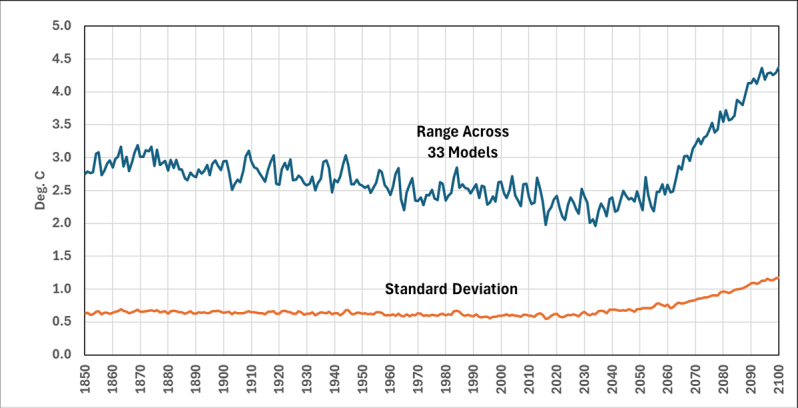
\includegraphics[width=.9\textwidth]{bilder/bilderKlima-0024.png}
  \captionof{figure}{CMIP6 Durchschnittliche Oberflächentemperaturspanne über 33 Modelle und Standardabweichung unter Verwendung des SSP5-85-Szenarios. Daten: KNMI Climate Explorer (\url{https://climexp.knmi.nl/start.cgi}).}
\end{minipage}

Jenseits der Fähigkeit der Modelle, Merkmale des heutigen Klimas zu reproduzieren, ist die kritische Frage für die Gesellschaft, wie gut sie Reaktionen auf subtile menschliche Einflüsse vorhersagen, wie Treibhausgasemissionen, Aerosol-Abkühlung und Landnutzungsänderungen. Der wichtigste Aspekt, den Modelle korrekt erfassen müssen, sind "Rückkopplungen". Diese treten auf, wenn Klimaänderungen entweder weitere Erwärmung verstärken oder unterdrücken. Im Allgemeinen verdoppelt oder verdreifacht der modellierte Nettoeffekt aller Rückkopplungen die direkte Erwärmungswirkung von CO$_2$.
\end{fullbox}

\section{Oberflächenerwärmung}
Ein einfacher Test der Gültigkeit eines Klimamodells ist seine Fähigkeit, historische Erwärmung als Reaktion auf bekannte vergangene Änderungen in Klimaantrieben wie Treibhausgasen zu reproduzieren. Abbildung 5.2 ist aus Scaffeta (2023) reproduziert, die die neueste Generation (CMIP6) von Klimamodellen in niedrige ECS ($1.5$ bis \SI{3.0}{\celsius}), mittlere ECS ($3.0$ bis \SI{4.5}{\celsius}) und hohe ECS ($4.5$ bis \SI{6.0}{\celsius}) gruppiert und ihre Post-1980 globalen Durchschnittstemperatur-Simulationsbereiche mit denen von drei Oberflächentemperaturaufzeichnungen und einem satelliten-basierten unteren Troposphärentemperatur-Datenprodukt vergleicht.
Die linke Spalte zeigt, dass die niedrig-ECS-Modelle die Post-1980 historische Erwärmungsaufzeichnung vernünftig gut verfolgen, aber die mittleren und rechten Spalten zeigen, dass die mittleren und hohen ECS-Modelle die Erwärmung auffällig über-vorhersagen.

\begin{figure}[H]
\begin{center}
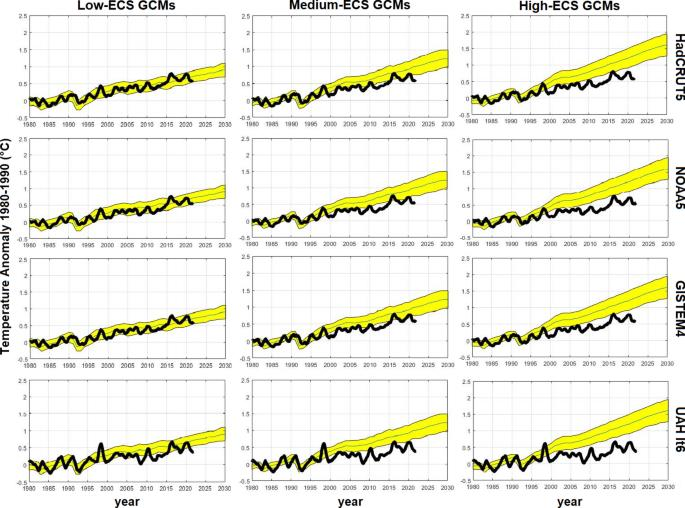
\includegraphics[width=1.0\textwidth]{bilder/bilderKlima-0026.jpg}\\[1cm]
\end{center}
\caption{Modell-Beobachtungs-Vergleiche für die Erwärmung der Erdoberfläche. Die Spalten entsprechen
Modellgruppen mit niedrigem ECS (13 Modelle), mittlerem ECS (11 Modelle) und hohem ECS (14 Modelle),
während die Zeilen den weit verbreiteten beobachteten Temperaturaufzeichnungen entsprechen, wobei die ersten drei
Oberflächendurchschnitte und die vierte den Durchschnitt der unteren Troposphäre zeigen. In jedem Feld bezeichnet der gelbe
Bereich den Mittelwert und die Spannweite (± eine Standardabweichung) der Klimamodellsimulationen für diese
Gruppe. Die dicke schwarze Linie zeigt die beobachtete jährliche Durchschnittstemperatur in der angegebenen Aufzeichnung.
Quelle: Scafetta (2023) Abb. 2.}
\end{figure}

Spencer (2024) hat auch eine nützliche Zusammenfassung der Modell-Beobachtungs-Diskrepanz bereitgestellt, indem er Trends in Oberflächentemperatur-Datenprodukten mit denen in einzelnen Klimamodellen verglich, wie in Abbildung 5.3 zusammengefasst; die meisten Klimamodelle zeigen erheblich mehr Erwärmung als die Beobachtungen seit 1979.

\begin{figure}[H]
\begin{center}
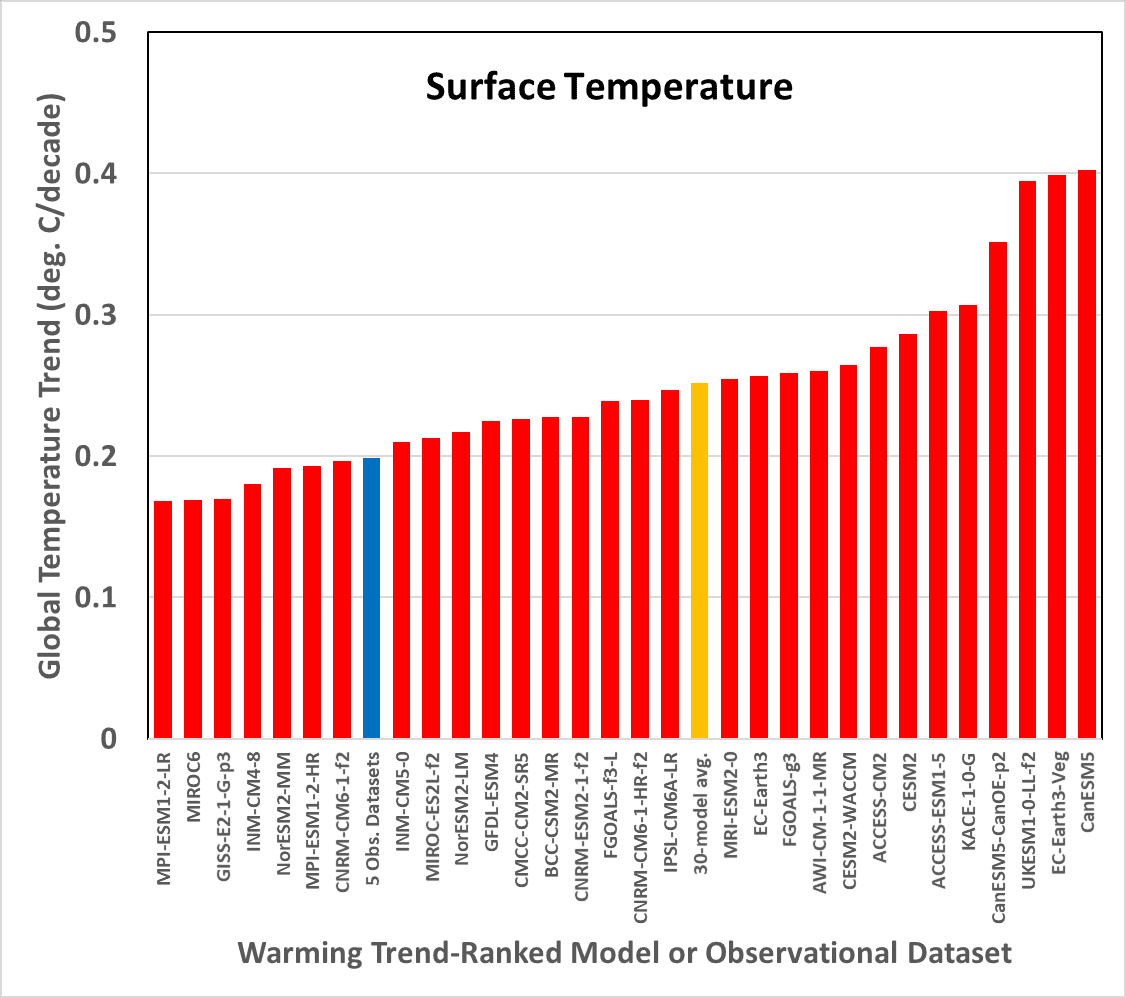
\includegraphics[width=1.0\textwidth]{bilder/bilderKlima-0027.png}\\[1cm]
\end{center}
\caption{Globale Trends der Oberflächenlufttemperatur (°C/Jahrzehnt), 1979–2024, aus verschiedenen CMIP6-Klimamodellen
(rot, Durchschnitt von 30 Modellen in orange); und der Durchschnitt von drei Thermometer-Datensätzen
(HadCRUT5, NOAA Global Temp und Berkeley 1 deg.) und zwei Reanalyse-Datensätzen (ERA5 und
NCEP/NCAR R1) in blau. Datenquelle: https://climexp.knmi.nl/start.cgi.}
\end{figure}

\section{Troposphärische Erwärmung}
Es ist seit langem bekannt, dass Klimamodelle im Durchschnitt die Erwärmung in der tropischen Troposphäre übertreiben. Diese Region ist ein wichtiger Test für Klimamodelle, da hier das Signal anthropogener Treibhauserwärmung zuerst und am stärksten auftritt. Verzerrungen in troposphärischen Trends zeigen Modellfehler in Wärmeübertragungsprozessen an, die sich auf Oberflächenerwärmungsverzerrungen übertragen.

Die Diskrepanz wurde als ernste Inkonsistenz im ersten U.S. Climate Change Science Program-Bericht (Karl et al. 2006) markiert und wurde in jedem IPCC-Bericht seitdem erwähnt, aber die Diskrepanz hat sich mit der Zeit verschlechtert, und die Verzerrung ist nun global. McKitrick und Christy (2020) verglichen troposphärische Erwärmungstrends in CMIP6-Klimamodellen mit beobachteten Trends von Satelliten, Wetterballons und Reanalysesystemen. Jedes Modell überschätzte den durchschnittlichen beobachteten Erwärmungstrend über 1979-2014 sowohl in unteren als auch mittleren Troposphärenschichten, sowohl global als auch in den Tropen. In den meisten einzelnen Modellen war die Verzerrung statistisch signifikant und im Durchschnitt über alle Modelle war sie hoch signifikant.

Abbildung 5.4 präsentiert die Vergleiche mit auf 2024 aktualisierten Daten (McKitrick und Christy 2025). Die jüngsten warmen Jahre bewegten den beobachteten Trend leicht nach oben und erweiterten die Trend-Konfidenzintervalle, aber das Gesamtmuster bleibt das gleiche: Modellverzerrung tendiert zu zu viel Erwärmung, in den meisten Fällen ist der Unterschied statistisch signifikant und im Durchschnitt ist die Verzerrung statistisch hoch signifikant. McKitrick und Christy (2020) zeigten auch, dass die Verzerrung in Modellen mit hoher ECS größer ist, aber selbst die Modelle mit niedrigerer durchschnittlicher ECS sagen zu viel Erwärmung vorher. Wenn zukünftige Klimamodelle globale troposphärische Erwärmung realistisch repräsentieren würden, wären sie wahrscheinlich weniger sensitiv als selbst die niedrig-ECS-Mitglieder des CMIP6-Ensembles.

\begin{figure}[H]
\begin{center}
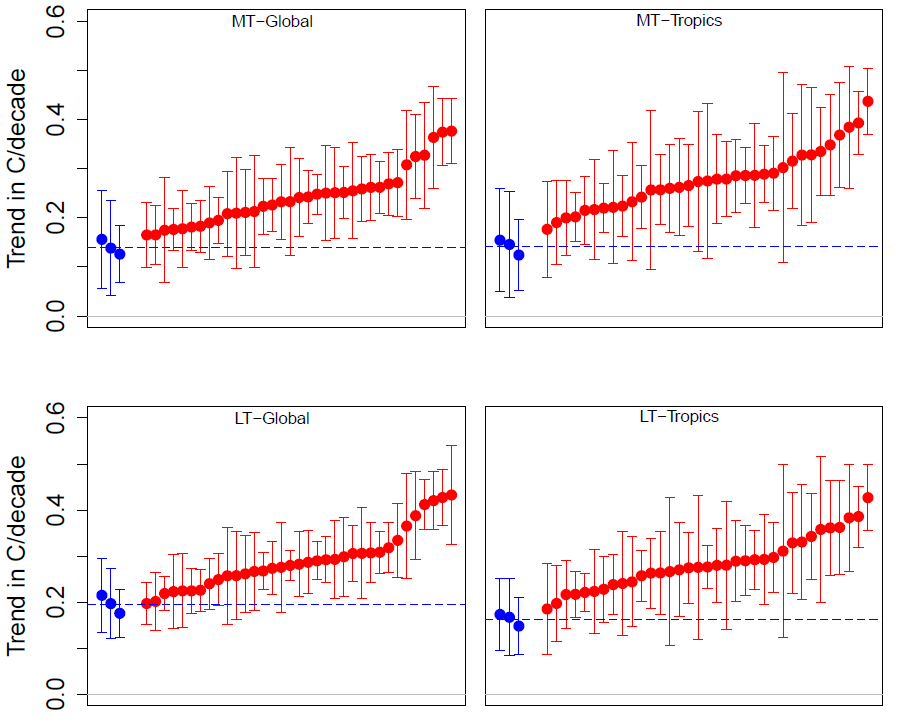
\includegraphics[width=1.0\textwidth]{bilder/bilderKlima-0028.png}\\[1cm]
\end{center}
\caption{Beobachtete gegenüber CMIP6-modellierten Erwärmungstrends (°C/Jahrzehnt 1979–2024) in der globalen
und tropischen unteren (LT) und mittleren Troposphäre (MT) unter Verwendung der Methodik von McKitrick und Christy
(2020) auf der Grundlage von Daten, die von 2014 bis 2024 aktualisiert wurden. Blaue Punkte: Erwärmungstrends mit 95-prozentigen Konfidenzintervallen
für 3 Datenprodukte (Radiosonden, Reanalyse und Satelliten). Blaue gestrichelte Linie: Durchschnittlicher Erwärmungstrend
für 3 beobachtete Reihen. Rote Punkte: Modellierte Erwärmungstrends mit 95-prozentigen Konfidenzintervallen
in 35 Modellen, angeordnet vom niedrigsten zum höchsten Wert.}
\end{figure}


Wie zuvor erwähnt, hat das IPCC die Modell-Beobachtungs-Diskrepanz lange anerkannt. Zum Beispiel bietet AR6 S. 443-444 dies zur tropischen Troposphäre (es behandelt nicht den globalen Vergleich):


\begin{quote}
Mehrere Studien seit AR5 haben weiterhin eine Inkonsistenz zwischen simulierten und beobachteten Temperaturtrends in der tropischen Troposphäre demonstriert, wobei Modelle mehr Erwärmung simulieren als Beobachtungen (Mitchell et al., 2013, 2020; Santer et al., 2017a, b; McKitrick und Christy, 2018; Po-Chedley et al., 2021)... Über den Zeitraum 1979–2014 sind Modelle konsistenter mit Beobachtungen in der unteren Troposphäre und am wenigsten konsistent in der oberen Troposphäre um 200 hPa, wo Verzerrungen \SI{0.1}{\celsius} pro Jahrzehnt überschreiten.
Mehrere Studien mit CMIP6-Modellen legen nahe, dass Unterschiede in der Klimasensitivität ein wichtiger Faktor sein könnten, der zur Diskrepanz zwischen simulierten und beobachteten troposphärischen Temperaturtrends beiträgt (McKitrick und Christy, 2020; Po-Chedley et al., 2021), obwohl es schwierig ist, den Einfluss von Klimasensitivität, Änderungen in Aerosolforcing und interner Variabilität bei der Beitragung zu troposphärischen Erwärmungsverzerrungen zu entschlüsseln (Po-Chedley et al., 2021). Eine andere Studie fand, dass das Fehlen einer hypothetischen negativen tropischen Wolkenrückkopplung die Hälfte der oberen Troposphären-Erwärmungsverzerrung in einem Modell erklären könnte (Mauritsen und Stevens, 2015).

... Zusammenfassend finden Studien weiterhin, dass CMIP5- und CMIP6-Modell\-simulationen mehr erwärmen als Beobachtungen in der tropischen mittleren und oberen Troposphäre über den Zeitraum 1979–2014 (Mitchell et al., 2013, 2020; Santer et al., 2017a, b; Suárez-Gutiérrez et al., 2017; McKitrick und Christy, 2018), und dass überschätzte Oberflächenerwärmung teilweise verantwortlich ist (Mitchell et al., 2013; Po-Chedley et al., 2021). ... Daher bewerten wir mit mittlerem Vertrauen, dass CMIP5- und CMIP6-Modelle weiterhin beobachtete Erwärmung in der oberen tropischen Troposphäre über den Zeitraum 1979–2014 um mindestens \SI{0.1}{\celsius} pro Jahrzehnt überschätzen.
\end{quote}

Bemerkenswert ist, dass trotz der Anhäufung von Belegen für überschüssige Modellerwärmung das IPCC nur mittleres Vertrauen in die Existenz einer Erwärmungsverzerrung zuordnet.

\section{Diskrepanz des vertikalen Temperaturprofils}
Eine weitere wichtige Modell-Beobachtungs-Diskrepanz ist die überschüssige Verstärkung mit der Höhe, die in Klimamodellen gefunden wird. Der Vergleich war in AR5 Kapitel 10, allerdings nur im Online-Supplement (Abbildung 10.SM.1) und nur in einer Abbildung, deren Formatierung den Punkt verdeckte. Abbildung 10.SM.1 wird weder im Haupt-IPCC-Bericht noch in irgendeiner Zusammenfassung referenziert, sodass Leser nicht davon gewusst hätten. Obwohl auf den ersten Blick nicht ersichtlich, zeigt sie, dass die Erwärmung von 1979-2010 in der unteren Troposphäre so gering ist, dass sie mit gar keinem THG-Forcing konsistent ist und inkonsistent mit den Modellläufen, die THG-Forcing haben. In Abbildung 5.6 adaptieren wir IPCC AR5 Abbildung 10.SM.1, um diesen kritischen Punkt herauszuarbeiten.

\begin{figure}[H]
\begin{center}
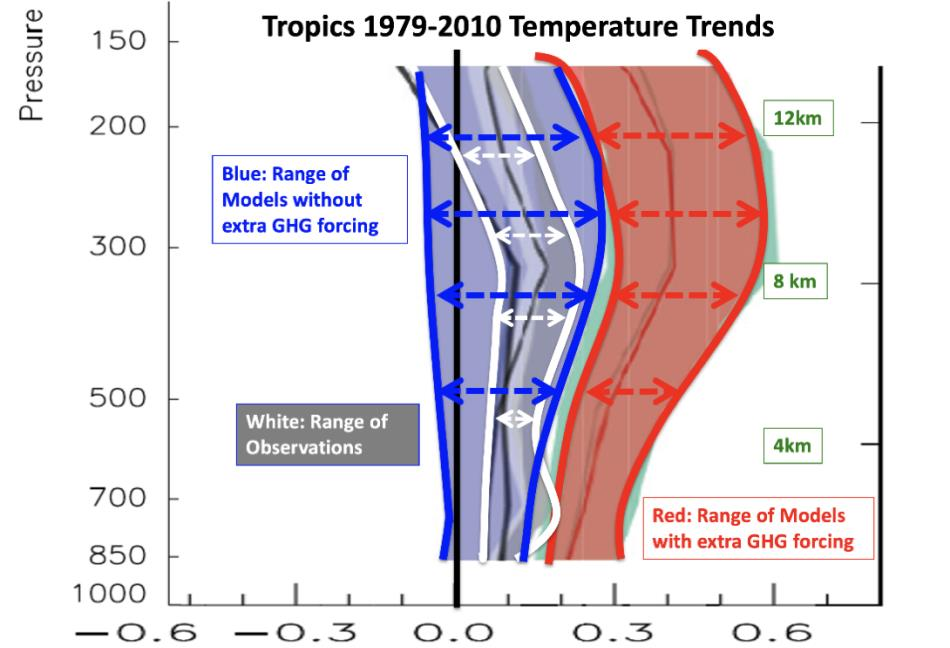
\includegraphics[width=1.0\textwidth]{bilder/bilderKlima-0029.jpg}\\[1cm]
\end{center}
\caption{Vertikales Erwärmungsmuster für die Tropen (\SI{20}{\degree}S bis \SI{20}{\degree}N). Horizontale Achse:
\si{\degree}/Jahrzehnt. Quelle: Kommentierte Version von IPCC AR5 Abbildung 10.SM.1}
\end{figure}

Abbildung 5.5 vergleicht Modell- und Beobachtungstemperaturtrends nach Höhe zwischen 20S und 20N (den Tropen). In dieser Region, wo die Modelle sagen, dass die Erwärmung am stärksten sein sollte, liegen die Beobachtungen (hier in weiß gezeigt) innerhalb des blauen \emph{Kein CO$_2$}-Bandes und völlig außerhalb der \emph{mit CO$_2$} roten Hülle. Das bedeutet, dass in der gesamten tropischen atmosphärischen Säule von der Oberfläche bis zur Basis der Stratosphäre beobachtete Erwärmungstrends so klein sind, dass sie mit der Ausgabe von Modellen konsistent sind, die kein anthropogenes CO$_2$ haben, und inkonsistent mit der gesamten Hülle von Erwärmungstrends, die von Modellen generiert werden, die mit erhöhtem CO$_2$ forciert werden.

Ein ähnlicher Vergleich wird in Christy und McNider (2017) gezeigt, eine aktualisierte Version davon (abdeckend 1979-2024) ist als Abbildung 5.6 reproduziert. Modellierte Temperaturtrends überschreiten Beobachtungen von der Oberfläche bis zur Spitze der Troposphäre, mit beobachteten Trends unterhalb des gesamten Modellbereichs auf den meisten Druckniveaus. Auch in Abbildung 5.6 gezeigt ist der tropische troposphärische Temperatur (TTT) Durchschnitt von drei Satellitendatenprodukten (NOAA, UAH und RSS) verglichen mit dem gleichen Schichtdurchschnitt von Klimamodellen für 1979-2024. Wieder liegen die beobachteten Trends unterhalb des gesamten Modellbereichs.

Die weite Spannweite der Entscheidungen, die von Modellierern getroffen werden, um die physikalischen Prozesse in den Modellen zu charakterisieren (siehe Kasten: Klimamodellierung in Abschnitt 5.1 oben), wird durch die große Streuung der Trends in der mittleren Troposphäre gesehen, ±40 Prozent um den Median (Abbildung 5.6). Dies illustriert lebhaft die Unsicherheiten in Versuchen, ein komplexes System zu modellieren (parametrisieren), das Turbulenz, feuchte Thermodynamik und Energieflüsse über den vollen Bereich der Zeit- und Raumskalen der tropischen Atmosphäre umfasst.

\begin{figure}[H]
\begin{center}
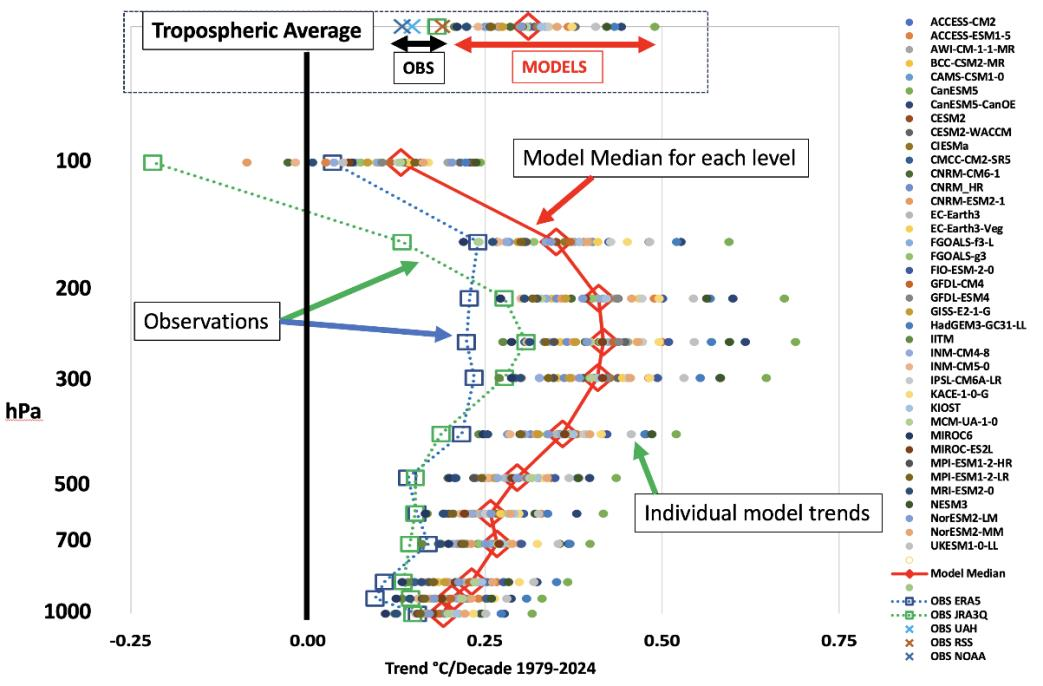
\includegraphics[width=1.0\textwidth]{bilder/bilderKlima-0030.jpg}\\[1cm]
\end{center}
\caption{Modellierte versus beobachtete Erwärmung, tropische Troposphäre. Quelle: aktualisiert
nach Christy und McNider (2017) einschließlich Daten bis 2024 und CMIP6-Modellausgaben.
Rote Linie: Modelldurchschnitt. Grüne und blaue Linien: Beobachtungsreihen (Reanalyse).}
\end{figure}

Diese Diskrepanz war die Quelle viel Kontroverse, wobei einige argumentierten, dass, selbst wenn es sehr wenig beobachtete Erwärmung in der Höhe in den Tropen gibt, ein "Hotspot" trotzdem existiert in dem Sinne, dass die Erwärmung in der Höhe größer ist als an der Oberfläche (Santer et al. 2008). Aber es gibt gute Belege, dass Modelle auch die Verstärkungsrate übertreiben. Klotzbach et al. (2009) zeigten, dass Modelle größere Verstärkung mit der Höhe projizieren, als beobachtet wird. Dieses Ergebnis wurde anschließend durch detaillierte Zeitreihenanalyse bestätigt (Vogelsang und Nawaz 2016), die fand, dass der Modell-Beobachtungs-Unterschied statistisch signifikant ist.
Das Temperaturprofil der Atmosphäre ist ein Fall, wo Modelle nicht nur unsicher sind, sondern auch eine gemeinsame Erwärmungsverzerrung relativ zu Beobachtungen zeigen. Das legt nahe, dass sie bestimmte fundamentale Rückkopplungsprozesse falsch darstellen.

Das IPCC AR6 bewertete dieses Problem nicht.


\section{Stratosphärische Abkühlung}
Ein wichtiges Element des erwarteten allgemeinen "Fingerabdrucks" des anthropogenen Klimawandels ist gleichzeitige Erwärmung der Troposphäre und Abkühlung der Stratosphäre. Das letztere Merkmal wird auch durch Ozonabbau und -erholung beeinflusst. AR6 anerkannte, dass Abkühlung beobachtet worden war, aber nur bis zum Jahr 2000. Die Stratosphäre hat seitdem eine gewisse Erwärmung gezeigt, entgegen Modellprojektionen.

AR6 WG1 Kap 2 S. 327-9 stellt fest:
\begin{quote}
Temperaturen, die über die gesamte untere Stratosphäre (etwa 10–25 km) gemittelt wurden, haben über 1980–2019 in allen Datenprodukten abgenommen, wobei der Großteil der Abnahme vor 2000 lag. Die Abnahme besteht auch, wenn der Einfluss der El Chichon (1982) und Pinatubo (1991) Vulkanausbrüche auf den Trend, von dem Steiner et al. (2020a) fanden, dass er den 1979–2018 Abkühlungstrend um \SI{0.06}{\celsius} pro Jahrzehnt erhöht hat, entfernt wird. Die meisten Datensätze zeigen keine signifikanten oder nur marginal signifikante Trends über 2000–2019, und die Ergebnisse von Philipona et al. (2018) zeigen schwache Zunahmen über 2000–2015 in der allertiefsten Stratosphäre, die von Radiosonden beprobt wird....

Es ist praktisch sicher, dass sich die untere Stratosphäre seit der Mitte des 20. Jahrhunderts abgekühlt hat. Jedoch zeigen die meisten Datensätze, dass sich untere stratosphärische Temperaturen seit Mitte der 1990er Jahre stabilisiert haben ohne signifikante Änderung über die letzten 20 Jahre. Es ist wahrscheinlich, dass sich mittlere und obere stratosphärische Temperaturen seit 1980 verringert haben, aber es gibt geringes Vertrauen in das Ausmaß.
\end{quote}

Die zitierte Quelle, Philipona et al. (2018), in einem Artikel mit dem Titel "Radiosonden zeigen, dass nach Jahrzehnten der Abkühlung sich die untere Stratosphäre jetzt erwärmt", stellte fest:
\begin{quote}
Als Reaktion auf fortgesetzte Treibhausgaserhöhungen und stratosphärischen Ozonabbau projizieren Klimamodelle fortgesetzte troposphärische Erwärmung und stratosphärische Abkühlung über die kommenden Jahrzehnte. Globale durchschnittliche Satellitenbeobachtungen unterer stratosphärischer Temperaturen zeigen keine signifikanten Trends seit der Jahrhundertwende. Im Gegensatz dazu zeigt eine Analyse vertikal aufgelöster Radiosondenmessungen von 60 Stationen eine Zunahme der unteren stratosphärischen Temperatur seit der Jahrhundertwende in Höhen zwischen 15 und 30 km und über den meisten Kontinenten. Trendschätzungen sind etwas empfindlich gegenüber Homogenitätsbewertungswahlmöglichkeiten, aber alle untersuchten Radiosondendatensätze legen eine Änderung von Abkühlung im späten zwanzigsten Jahrhundert zu Erwärmung im frühen 21. Jahrhundert in der unteren Stratosphäre nahe.
\end{quote}

Santer et al. (2023) verwenden aktualisierte Daten, um zu zeigen, dass ein Abkühlungstrend in der unteren Stratosphäre nicht wieder aufgetaucht ist.

Eine Kombination aus troposphärischer Erwärmung und stratosphärischer Abkühlung ist ein häufig zitierter "Fingerabdruck" des anthropogenen Klimawandels. Stratosphärische Erwärmung seit 2000 fällt mit fortgesetzter Oberflächen- und troposphärischer Erwärmung zusammen, ein Muster, das in Klimamodellsimulationen nicht gefunden wird und anscheinend nicht konsistent mit dem anthropogenen Fingerabdruck ist.

\section{Diskrepanz der Schneebedeckung}
Daten, die vom Rutgers University Snow Lab zusammengestellt wurden, zeigen, dass die Winterschneebedeckung der Nordhemisphäre nicht abnimmt (Abbildung 5.7); wenn überhaupt, zeigt sie einen zunehmenden Trend.

\begin{figure}[H]
\begin{center}
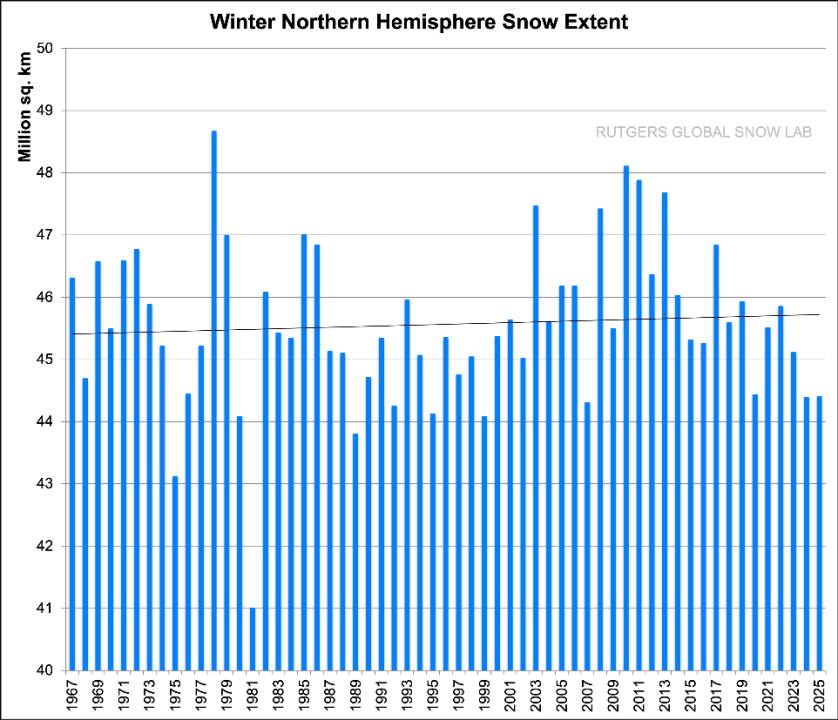
\includegraphics[width=1.0\textwidth]{bilder/bilderKlima-0031.png}\\[1cm]
\end{center}
\caption{Schneebedeckung im Winter auf der Nordhalbkugel.
Quelle: \url{https://climate.rutgers.edu/snowcover/chart_seasonal.php?ui_set=nhland&ui_season=1}
(abgerufen am 27. Mai 2025)}
\end{figure}

Dennoch projizieren Modelle abnehmende Schneebedeckung der Nordhemisphäre in einem sich erwärmenden Klima, wie von Connolly et al. (2019) beschrieben.
\begin{quote}
Es wurde gefunden, dass die Klimamodelle die beobachteten Trends [in der Schneebedeckung der Nordhemisphäre] schlecht erklären. Während die Modelle nahelegen, dass Schneebedeckung für alle vier Jahreszeiten stetig hätte abnehmen sollen, zeigten nur Frühling und Sommer eine langfristige Abnahme, und das Muster der beobachteten Abnahmen für diese Jahreszeiten war ziemlich unterschiedlich von den modellierten Vorhersagen. Darüber hinaus legen die beobachteten Trends für Herbst und Winter eine langfristige Zunahme nahe, obwohl diese Trends nicht statistisch signifikant waren.
\end{quote}

AR6 beschränkt seine Diskussion der sich ändernden Schneebedeckungsausdehnung (SCE) der Nordhemisphäre weitgehend auf die Frühlingssaison, für die Modelle und Beobachtungen in einem Abwärtstrend übereinstimmen. Bezüglich Winteränderungen bemerkt es wie folgt (AR6 WGI Kap. 2 S. 344):
\begin{quote}
Die Bewertung von SCE-Trends in der NH seit 1978 zeigt, dass für den Oktober bis Februar Zeitraum erhebliche Unsicherheit in Trends besteht, wobei das Vorzeichen vom Beobachtungsprodukt abhängt. Analyse mit dem NOAA Climate Data Record zeigt eine Zunahme in Oktober bis Februar SCE (Hernández-Henríquez et al., 2015; Kunkel et al., 2016), während Analysen basierend auf satellitengetragenen optischen Sensoren (Hori et al., 2017) oder Multi-Beobachtungsprodukten (Mudryk et al., 2020) einen negativen Trend für alle Jahreszeiten zeigen.
\end{quote}

AR6 WGI Kapitel 9 (S. 1284) weist darauf hin, dass der NOAA Climate Data Record, der erhöhte Herbst- und Winter-SCE zeigt, inkonsistent mit landbasierten Beobachtungen und modellbasierten Datensätzen ist. Es bemerkt, dass die Verwendung optischer Satellitenbilder zur Ableitung von SCE im Winter aufgrund von Wolkenbedeckung und verringerter Sonnenbeleuchtung in Wintermonaten herausfordernd ist. Mit Fokus auf die Pazifikküstenstaaten (CA, OR und WA) stellt kaltsaisonaler Bergschneefall, der im Frühling und Sommer schmilzt, einen erheblichen Teil der warmsaisonalen Wasserressourcen bereit.
Eine umfassende Rekonstruktion des Schneefalls für die Hauptquellregionen (Cascade- und Sierra-Nevada-Berge) zeigt keine signifikanten Trends in jährlichen Gesamtsummen seit dem späten 19. Jahrhundert (Christy 2022).

Zusammenfassend zeigt die aktuelle Rutgers SCE-Datenbank eine Diskrepanz zwischen Modellen und Beobachtungen an. Weitere Arbeit zur Versöhnung widersprüchlicher Trends in Beobachtungsdatensätzen ist erforderlich.

\section{Hemisphärische Symmetrie der planetaren Albedo}
Die planetare Albedo ist der Anteil der einkommenden Sonnenstrahlung, der von der Erde zurück in den Weltraum reflektiert wird. Sie ist ein wichtiges Element der strahlenden Energiebilanz und beeinflusst, ob sich der Planet über die Zeit erwärmen oder abkühlen wird. Die planetare Albedo wird typischerweise auf etwa 0,30 geschätzt; Variationen im Maßstab von 0,01 entsprechen Änderungen im Solarforcing von etwa \SI{3}{\watt\per\square\meter}, einem Betrag, der größer ist als das aktuelle anthropogene Forcing. Es wurde seit langem bemerkt, dass Modelle untereinander und mit Beobachtungen über den Wert der globalen planetaren Albedo uneinig sind (Stephens et al. 2015).

Eine faszinierende Eigenschaft der Erdalbedo ist, dass im Durchschnitt die Nordhemisphäre (NH) und Südhemisphäre (SH) nahezu die gleiche Albedo hatten, zumindest während der fünfzigjährigen Satellitenaufzeichnung (Stephens et al., 2015). Diese Symmetrie ist überraschend, weil die SH viel mehr Ozean als Land hat. Da Ozean weniger reflektierend ist als Land, sollte die NH höhere Albedo haben. Wolken (die hochreflektierend sind) sind in der NH häufiger und kompensieren so die Oberflächenalbedo-Ungleichgewichte der zwei Hemisphären. Datseris und Stephens (2021) zeigen, dass diese Wolkenkompensation von den außertropischen Sturmbahnen der SH kommt, die wolkiger sind als die der NH. Während der Mechanismus für diese hemisphärische Symmetrie unklar ist, operiert er wahrscheinlich auf großen zeitlichen und räumlichen Skalen.

Die hemisphärische Symmetrie der Albedo ist eine einfache grobe Metrik für Klimamodelle. Rugenstein und Hakuba (2023) definierten diese Metrik als den Unterschied zwischen den jährlichen Mittelalbedos von NH und SH, ausgedrückt als \si{\watt\per\square\meter} des reflektierten Sonnenlichts, und stellten sie für die CMIP6-Klimamodelle zusammen, wie in Abbildung 5.8 gezeigt. Die meisten CMIP6-Modelle reproduzieren die kleine beobachtete Asymmetrie (etwa \SI{0.1}{\watt\per\square\meter}) nicht und sind sich sogar uneinig darüber, welche Hemisphäre reflektierender ist. Darüber hinaus reicht das Ausmaß der Asymmetrie in einigen Modellen bis zu \SI{5}{\watt\per\square\meter}, zweimal so groß wie das aktuelle anthropogene Forcing (etwa \SI{2.7}{\watt\per\square\meter}).

Die Bedeutung unphysikalischer Albedo-Asymmetrien in den Klimamodellen ist noch nicht vollständig bekannt. Jedoch legen andere Modellstudien nahe, dass interhemisphärische Änderungen in der Albedo polwärtige Wärmeflüsse, meridionale Temperaturgradienten, Sturmhäufigkeit und Unterschiede in hemisphärischer ozeanischer Wärmespeicherung verändern können. Die Diskrepanz zwischen Modellen und Beobachtungen wirft weitere Fragen bezüglich Wolken-Rückkopplungsprozessen auf und verringert so allgemeiner das Vertrauen in Modellprojektionen des zukünftigen Klimas.
\begin{figure}[H]
\begin{center}
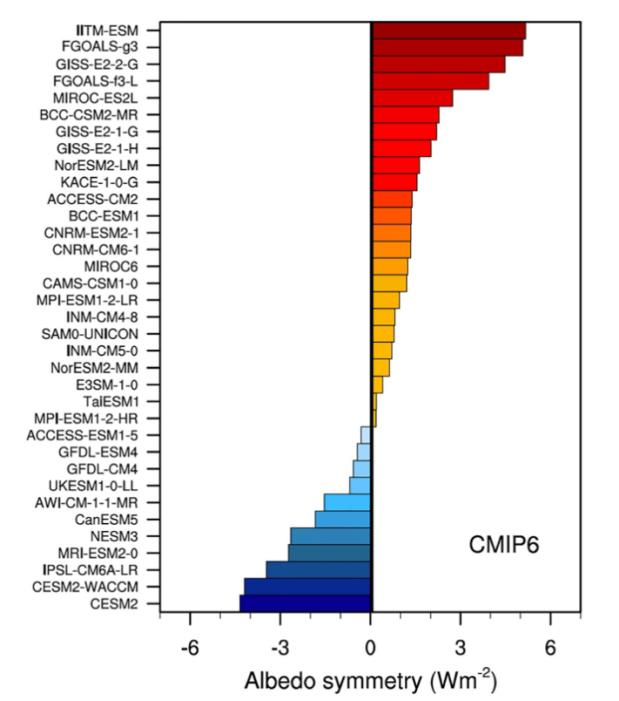
\includegraphics[width=1.0\textwidth]{bilder/bilderKlima-0033.jpg}\\[1cm]
\end{center}
\caption{Unterschiede in der durchschnittlichen Reflektivität (Albedo) über 20 Jahre zwischen der nördlichen und
südlichen Hemisphäre für CMIP6-Modelle, die in der jüngsten IPCC-Bewertung verwendet wurden (farbige Balken).
Der sehr geringe beobachtete Unterschied wird durch die vertikale schwarze Linie angezeigt. Aus Rugenstein und
Hakuba (2023).}
\end{figure}

\section{U.S. Corn Belt}
Eine der größten Diskrepanzen zwischen Modellen und Beobachtungen liegt im U.S. Corn Belt, einer Region von besonderer Bedeutung für die globale Nahrungsmittelproduktion. Abbildung 5.9 zeigt die Erwärmungstrends für die Sommerzeit (Juni, Juli, August) für den 12-Staaten Corn Belt (IN, IA, IL, ND, SD, MO, MN, WI, MI, OH, KS, NE) während 1973-2022. Alle 36 Klimamodelle (rot) erwärmen sich viel zu schnell verglichen mit Beobachtungen (blau).

\begin{figure}[H]
\begin{center}
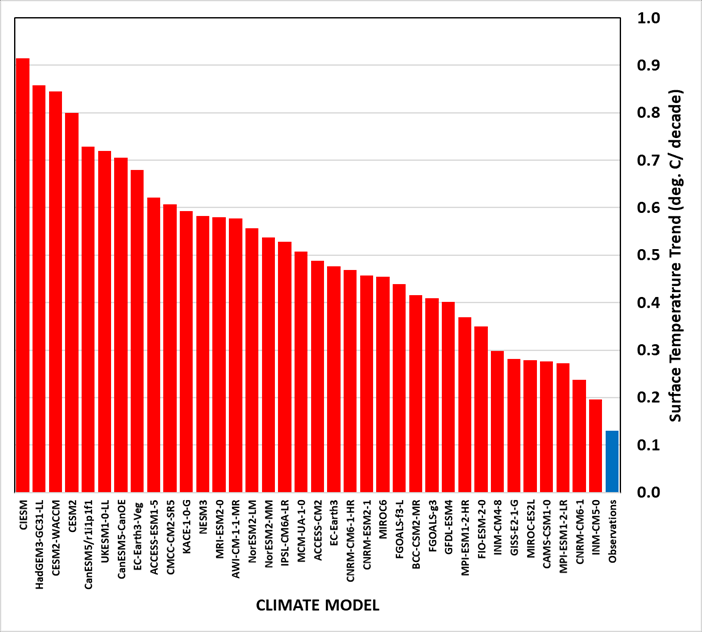
\includegraphics[width=1.0\textwidth]{bilder/bilderKlima-0034.png}\\[1cm]
\end{center}
\caption{Modellierte versus beobachtete Erwärmungstrends im US-amerikanischen Maisgürtel, 1973–2022.}
\end{figure}

Wie in Kapitel 9 diskutiert, sind die erwarteten negativen Effekte steigender Temperaturen auf U.S. Maiserträge nicht eingetreten, im Gegensatz zu weit publizierten Studien, die proklamieren, dass theoretische zukünftige Auswirkungen bereits erfahren werden (z.B., Seager et al., 2018).

Das IPCC erkennt Begrenzungen in der Genauigkeit regionaler Klimamodell-Ausgaben an. Dieses Beispiel zeigt, dass Nutzer Modellprojektionen sorgfältig von Fall zu Fall bewerten müssen, da lokale Verzerrungen möglicherweise ausreichend groß sind, dass die Modelle einfach nicht für den Zweck geeignet sind. Wie kürzlich von zwei Führern der Modellierungsgemeinschaft bemerkt wurde (Hervorhebung hinzugefügt):
\begin{quote}
... für viele Schlüsselanwendungen, die regionale Klimamodell-Ausgaben erfordern oder für die Bewertung großmaßstäblicher Änderungen aus kleinmaßstäblichen Prozessen, glauben wir, dass die aktuelle Generation von Modellen nicht für den Zweck geeignet ist. (Palmer und Stevens 2019)
\end{quote}

Zusammenfassend:
\begin{itemize}
\item Klimamodelle zeigen Erwärmungsverzerrungen in vielen Aspekten ihrer Reproduktion der vergangenen wenigen Jahrzehnte.
\item  Sie produzieren zu viel Erwärmung an der Oberfläche (außer in den Modellen mit niedrigster ECS), zu viel Erwärmung in der unteren und mittleren Troposphäre und zu viel Verstärkung der Erwärmung in der Höhe.
\item  Sie produzieren auch zu viel stratosphärische Abkühlung, zu viel Schneeverlust und zu viel Erwärmung im U.S. Corn Belt.
\item  Der hemisphärische Albedo-Unterschied in einzelnen Klimamodellen reicht weit in Vorzeichen und Größenordnung verglichen mit Beobachtungen. Der Bereich in \si{\watt\per\square\meter} ist dreimal größer als das direkte anthropogene Forcing von CO$_2$.
\item  Das IPCC hat einige dieser Probleme anerkannt, aber nicht alle.
\end{itemize}

\vfill
\noindent\textbf{Literaturverzeichnis:}

\begingroup
\parindent=0pt
\everypar{\hangindent=2em\hangafter=1\relax}

Christy, J. R., R. T. McNider (2017). Satellite bulk tropospheric temperatures as a metric for climate
sensitivity. Asia-Pacific Journal of Atmospheric Sciences 53, 511-518.
https://doi.org/10.1007/s13143-017-0070-z

Christy, J. R. (2022). Time series construction of Oregon and Washington snowfall since 1890 and an
update of California snowfall through 2020. Journal of Hydrometeorology 23, 1845-1860.
https://doi.org/10.1175/JHM-D-21-0178.1

Connolly, R., M. Connolly, W. Soon, et al. (2019). Northern Hemisphere snow-cover trends (1967–
2018): A comparison between climate models and observations. Geosciences 9, 135.
https://doi.org/10.3390/geosciences9030135

Datseris, G., B. Stevens (2021). Earth’s albedo and its symmetry. AGU Advances 2,
e2021AV000440. https://doi.org/10.1029/2021AV000440

Karl, T.R., S. J. Hassol, C. D. Miller, W. L. Murray, eds. (2006). Temperature Trends in the Lower
Atmosphere: Steps for Understanding and Reconciling Differences. U.S. Climate Change Science
Program/Subcommittee on Global Change Research.
\url{https://digital.library.unt.edu/ark:/67531/metadc12017/m2/1/high_res_d/sap1-1-final-all.pdf}

Klotzbach, P.J., R. A. Pielke, Sr., R. A. Pielke, Jr., J. R. Christy, R. T. McNider (2009). An alternative
explanation for differential temperature trends at the surface and in the lower troposphere.
Journal of Geophysical Research — Atmospheres 114(D21).
\url{https://doi.org/10.1029/2009JD011841}

McKitrick, R. and J. R. Christy (2020). Pervasive warming bias in CMIP6 tropospheric layers. Earth and
Space Science 7. https://doi.org/10.1029/2020EA001281

McKitrick, R., and J.R. Christy (2025), “Data and Code for DoE Report 2025”, Mendeley Data, V1, doi:
10.17632/8n9ks93vn7.1

Palmer, T., and B. Stevens (2019). The scientific challenge of understanding and estimating climate
change. Proceedings of the National Academy of Sciences 116(49), 24390–24395.
https://doi.org/10.1073/pnas.1906691116

Philipona, R., C. Mears, M. Fujiwara, et al. (2018). Radiosondes show that after decades of cooling, the
lower stratosphere is now warming. Journal of Geophysical Research—Atmospheres 123.
https://doi.org/10.1029/2018JD028901

Rugenstein, M., and M. Hakuba (2023). Connecting hemispheric asymmetries of planetary albedo and
surface temperature. Geophysical Research Letters 50, e2022GL101802.
https://doi.org/10.1029/2022GL101802

Santer B D, P.W. Thorne, L Haimberger et al. (2008) Consistency of modelled and observed temperature
trends in the tropical troposphere International Journal of Climatology 28 1703–22
https://rmets.onlinelibrary.wiley.com/doi/abs/10.1002/joc.1756


Santer, B.D. S. Po-Chedley, L. Zhao, C et al. (2023) Exceptional stratospheric contribution to human
fingerprints on atmospheric temperature, Proceedings of the National Academy of Sciences U.S.A. 120
(20) e2300758120, https://doi.org/10.1073/pnas.2300758120.

Scaffeta, N (2023) CMIP6 GCM ensemble members versus global surface temperatures. Climate Dynamics
60, 3091–3120 (2023). https://doi.org/10.1007/s00382-022-06493-w

Seager, R., J. Feldman, N. Lis, et al. (2017). Whither the 100th meridian? The once and future physical
and human geography of America’s arid–humid divide. Part II: The meridian moves east. Earth
Interactions 22. https://doi.org/10.1175/EI-D-17-0012.1

Spencer, R. W. (2024). Global warming: Observations vs. climate models. Environment Backgrounder,
The Heritage Foundation.
https://www.heritage.org/environment/report/global-warming-observations-vs-climate-models

Stephens, G. L., D. O'Brien, P.J. Webster et al. (2015). The albedo of Earth. Reviews of Geophysics.
https://doi.org/10.1002/2014RG000449

Vogelsang, T. and N. Nawaz (2016). Estimation and inference of linear trend slope ratios with an
application to global temperature data: Journal of Time Series Analysis 38.
https://doi.org/10.1111/jtsa.12209
\endgroup

\cleardoublepage
\FigureNumbersBySection
\chapter{Extrem Wetter}
\paragraph{Kapitelzusammenfassung}
\begin{quote}
Die meisten Arten von Extremwetter zeigen keine statistisch signifikanten langfristigen Trends über die verfügbare historische Aufzeichnung. Während es eine Zunahme heißer Tage in den USA seit den 1950er Jahren gegeben hat, ein Punkt, der von AR6 betont wird, sind die Zahlen immer noch niedrig relativ zu den 1920er und 1930er Jahren. Extreme konvektive Stürme, Hurrikane, Tornados, Überschwemmungen und Dürren zeigen beträchtliche natürliche Variabilität, aber langfristige Zunahmen werden nicht erkannt.
Einige Zunahmen in extremen Niederschlagsereignissen können in einigen Regionen über kurze Intervalle erkannt werden, aber die Trends bestehen nicht über lange Zeiträume und auf regionaler Ebene fort. Waldbrände sind in den USA nicht häufiger als sie in den 1980er Jahren waren. Die verbrannte Fläche nahm von den 1960er Jahren bis zu den frühen 2000er Jahren zu, sie ist jedoch niedrig verglichen mit dem geschätzten natürlichen Grundniveau. Die US-Waldbrandaktivität wird stark von Forstwirtschaftspraktiken beeinflusst.
\end{quote}

\section{Einleitung}
Wetterextreme mit hohem Einfluss, die gewöhnlich mit Temperatur, Niederschlag und/oder starkem Wind zusammenhängen, können Infrastruktur stören und daher die menschliche Gesundheit und das Wohlbefinden gefährden. Die Frage ist nicht, ob Extreme auftreten. Vielmehr ist es, ob es langfristige (dekadische) Änderungen in der Häufigkeit oder dem Charakter von Extremen gibt ("Detektion"), sowie das Ausmaß, in dem solche Änderungen und die damit verbundenen Änderungen in Gefahren durch anthropogene Emissionen von Treibhausgasen verursacht werden ("Attribution"; z.B., AR6 Seneviratne et al. 2021).

Prozessbasiertes Verständnis und einfache thermodynamische Argumente sind herangezogen worden, um zu behaupten, dass Erwärmung Extremwetterereignisse verschlechtert. Es ist jedoch naiv anzunehmen, dass jedes jüngste Extremereignis durch menschliche Einflüsse auf das Klima verursacht wird. Klima handelt von den statistischen Eigenschaften des Wetters über Jahrzehnte, nicht von einzelnen Ereignissen. Weiterhin gibt es nur etwa 130 Jahre zuverlässiger Beobachtungsaufzeichnungen, die statistisch analysiert werden können. Dieses kurze Intervall beginnt nicht einmal, alle Extremereignisse zu enthalten, die das Klimasystem von allein erzeugen kann. Über geologische Zeit hat das Klimasystem eine (im Wesentlichen) unendliche Vielfalt von Wettermustern und Extremen erzeugt, die Menschen nie beobachtet haben und die daher in den Datenbanken fehlen, die zur Bestimmung extremer Statistiken verwendet werden [siehe Gefahren kurzer Datenaufzeichnungen unten]. Aus diesem Grund erfordert die Attribution eines Extremereignisses, das in der Aufzeichnung beispiellos ist, Annahmen über das Ausmaß natürlicher Variationen.

Dieses Kapitel befasst sich mit der Detektion von Trends im Extremwetter, während Kapitel 8 kausale Attribution betrachtet, mit Abschnitt 8.4, der sich spezifisch mit Extremwetter befasst. Wenn kein Trend erkannt wird, dann gibt es klar keine Basis für Attribution. Aber selbst wo ein Trend beobachtet wird, folgt Attribution zu menschlich verursachter Erwärmung nicht notwendigerweise.

Das ist besonders wahr für Niederschlagsereignisse. Die hydrologische Literatur hat seit langem das Vorhandensein langer, langsamer und unregelmäßiger Oszillationen in Niederschlagsdaten bemerkt (Hurst 1951, Cohn und Lins 2005, Markonis und Koutsoyiannis 2016). Die Charakteristika dieser natürlichen Muster erfordern lange Aufzeichnungen, um Variabilität genau zu schätzen. Analyse von Aufzeichnungen, die kurz sind relativ zur Skala natürlicher Variabilität, wird dazu tendieren, Trends falsch darzustellen, daher die Signifikanz scheinbarer Trends zu übertreiben und die Wahrscheinlichkeit von Extremereignissen zu unterschätzen (Cohn und Lins 2005).

\begin{figure}[H]
\begin{center}
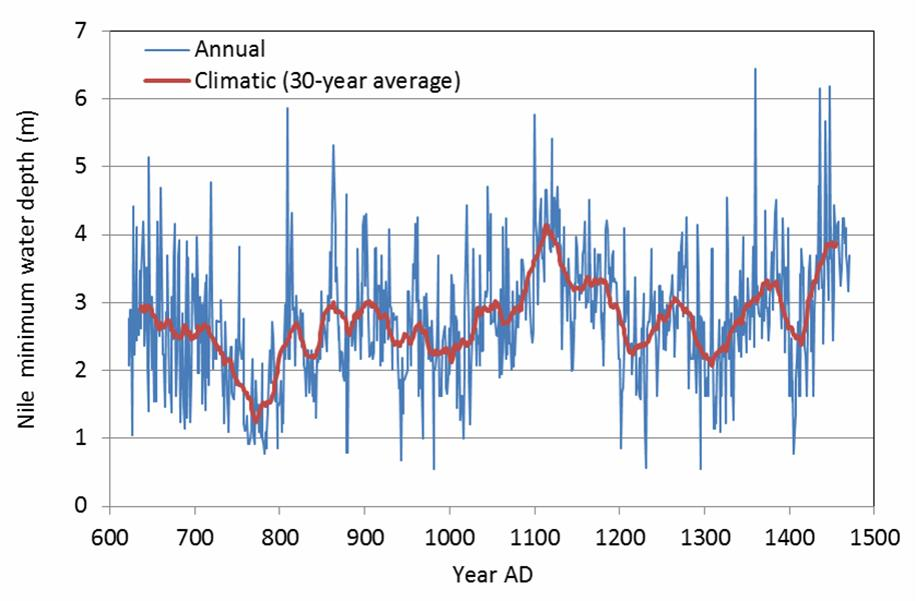
\includegraphics[width=1.0\textwidth]{bilder/bilderKlima-0036.jpg}\\[1cm]
\end{center}
\caption{Die jährliche Mindesttiefe des Nils in der Nähe von Kairo über einen Zeitraum von mehr als 650
Jahren von 622 bis 1284 n. Chr. Die in Metern gemessenen Daten zeigen ein charakteristisches Muster
von jährlichen Schwankungen um längerfristige Trends herum. Daten von Koutsoyiannis (2013)}
\end{figure}

Ein gutes Beispiel dafür ist die acht Jahrhunderte lange Aufzeichnung der jährlichen Mindesthöhe des Nils, die auf der Roda-Insel in Kairo beobachtet wurde, gezeigt in Abbildung 6.1.1. Der Nil wird von Niederschlag über ein 4 Millionen Quadratmeilen großes Einzugsgebiet gespeist, ein Gebiet gleich etwa einem Drittel von CONUS. Da menschliche Einflüsse auf das globale Klima lange vor dem 20. Jahrhundert vernachlässigbar waren, ist die jahrhundertliche Variabilität des dreißigjährigen Durchschnitts völlig natürlich; Ägypter des siebten und achten Jahrhunderts wären falsch gelegen anzunehmen, dass die sich verschlechternde Dürre während dieser Zeit das \emph{neue Normal} war.

Mit diesen Vorbehalten im Hinterkopf untersuchen wir die Belege für Änderungen in ausgewählten Wetter- und Klimaextremen. Ein wiederkehrendes Thema ist die weite Kluft zwischen öffentlichen Wahrnehmungen und wissenschaftlichen Belegen. Es ist routinemäßig in Medienberichterstattung, Regierungs- und Privatsektor-Diskussionen und sogar in etwas akademischer Literatur geworden, verallgemeinerte Behauptungen aufzustellen, dass Extremwetter aller Arten aufgrund von THG und \emph{Klimawandel} schlimmer wird. Dennoch haben Expertenbewertungen typischerweise keine solch umfassenden Schlussfolgerungen gezogen und haben stattdessen die Schwierigkeit betont, sowohl spezifische Trends zu identifizieren als auch eine kausale Verbindung mit anthropogener Forcierung zu etablieren.

In den folgenden Abschnitten liefern wir Auszüge aus verschiedenen IPCC- und NCA-Bewertungsberichten, wobei wir die Quellen wie folgt bezeichnen:
\begin{description}
\item[SREX:] Der IPCC-Sonderbericht über die Bewältigung der Risiken von Extremereignissen und Katastrophen zur Förderung der Anpassung an den Klimawandel (2012)
\item[AR6:] Der IPCC Sechste Bewertungsbericht Arbeitsgruppe 1 (2021). 
\item[NCA4:] Der U.S. Climate Science Special Report des Vierten Nationalen Klimabewertung (2017) Band I.
\item[NCA5:] Fünfte Nationale Klimabewertung (2023).
\end{description}

In den Auszügen sind \emph{Kursivschrift} im Original, während \textbf{Fettdruck} zur Betonung hinzugefügt wurde.

Zusätzlich verwenden wir standardmäßige Regierungsquellen, um Informationen bis 2024 zu liefern, wo immer möglich.

\section{Hurrikans und Tropische Wirbelstürme}
AR6 liefert die folgende Bewertung tropischer Wirbelstürme (TCs; hier als Synonym für Hurrikans verwendet):
\begin{quote}
AR6: Es besteht geringes Vertrauen in die meisten berichteten langfristigen (multidekadischen bis säkularen) Trends bei der Häufigkeit oder intensitätsbasierten Metriken tropischer Wirbelstürme aufgrund von Änderungen in der Technologie, die zur Sammlung der Best-Track-Daten verwendet wird. (IPCC, 2021 S. 1585)

AR6: Es ist wahrscheinlich, dass der globale Anteil schwerer Tropenwirbelstürme (Kategorie 3–5) in den letzten vier Jahrzehnten zugenommen hat... Es besteht geringes Vertrauen in langfristige (multidekadische bis säkulare) Trends bei der Häufigkeit aller Kategorien von Tropenwirbelstürmen. (IPCC, 2023 SPM S. 9)

AR6: Eine Teilmenge der Best-Track-Daten, die Hurrikans entspricht, die die Vereinigten Staaten seit 1900 direkt beeinflusst haben, wird als zuverlässig betrachtet und zeigt \textbf{keinen Trend in der Häufigkeit von US-Landfallereignissen}. (IPCC 2021 S. 1585)
\end{quote}

Seit 1980, als Satellitenbeobachtungen erstmals die globalen Ozeane vollständig abdeckten, haben wir Vertrauen in die Zahlen der gesamten globalen Hurrikans und schweren Hurrikans (Kategorie 3 und höher). Abbildung 6.2.1 zeigt, dass es im Durchschnitt etwa 50 Hurrikans pro Jahr gibt, von denen etwa 25 den Status schwerer Hurrikans erreichen (Maue, 2025). Es gibt erhebliche Jahr-zu-Jahr- und dekadische Variabilität, eine schwache Abnahme der Anzahl von Hurrikans und einen leichten, aber nicht signifikanten Anstieg der Anzahl schwerer Hurrikans. Diese beiden Trends kombinieren sich zu einem allgemeinen Anstieg des Anteils schwerer Hurrikans.

Die globalen Hurrikan-Statistiken werden vom Nordwestpazifik dominiert, der etwa 35 Prozent aller globalen Hurrikans ausmacht, während der Atlantik etwa 15 Prozent der globalen Hurrikans ausmacht (Colorado State University, 2025). Die Daten im Atlantikbecken reichen weiter zurück als in den anderen Ozeanbecken und sind für US-Politiker am relevantesten.

\begin{figure}[H]
\begin{center}
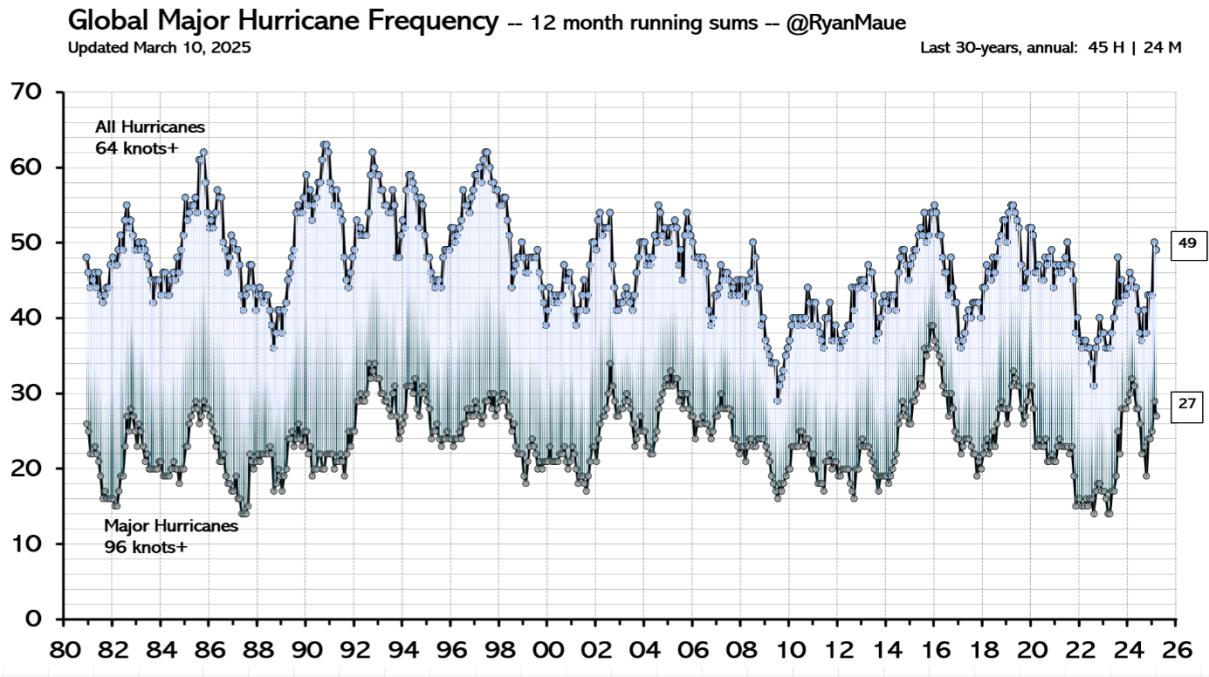
\includegraphics[width=1.0\textwidth]{bilder/bilderKlima-0037.jpg}\\[1cm]
\end{center}
\caption{Globale Häufigkeit von Hurrikans und schweren Hurrikans seit 1980. Quelle: Aktualisiert von Maue 2011.}
\end{figure}

Abbildung 6.2.2 zeigt die Häufigkeit atlantischer Hurrikans und schwerer Hurrikans (Kategorie 3 und höher) zurück bis 1920. Daten vor 1965 (dem Beginn der Satellitenbeobachtungen im Atlantik, blau schattiert) zeigen eine gewisse Unterzählung, wobei Daten vor 1920 erhebliche Unterzählung zeigen (Vecchi und Knutson, 2011). Alle Messgrößen atlantischer Hurrikan-Aktivität zeigen einen signifikanten Anstieg seit 1970. Jedoch sah der Zeitraum von 1971-1994 außergewöhnlich niedrige Aktivität, wobei hohe Aktivität (vergleichbar mit den letzten zwei Jahrzehnten, sogar bei Unterzählung) auch in den 1950er und 1960er Jahren und sogar in den 1930er Jahren beobachtet wurde.

\begin{figure}[H]
\begin{center}
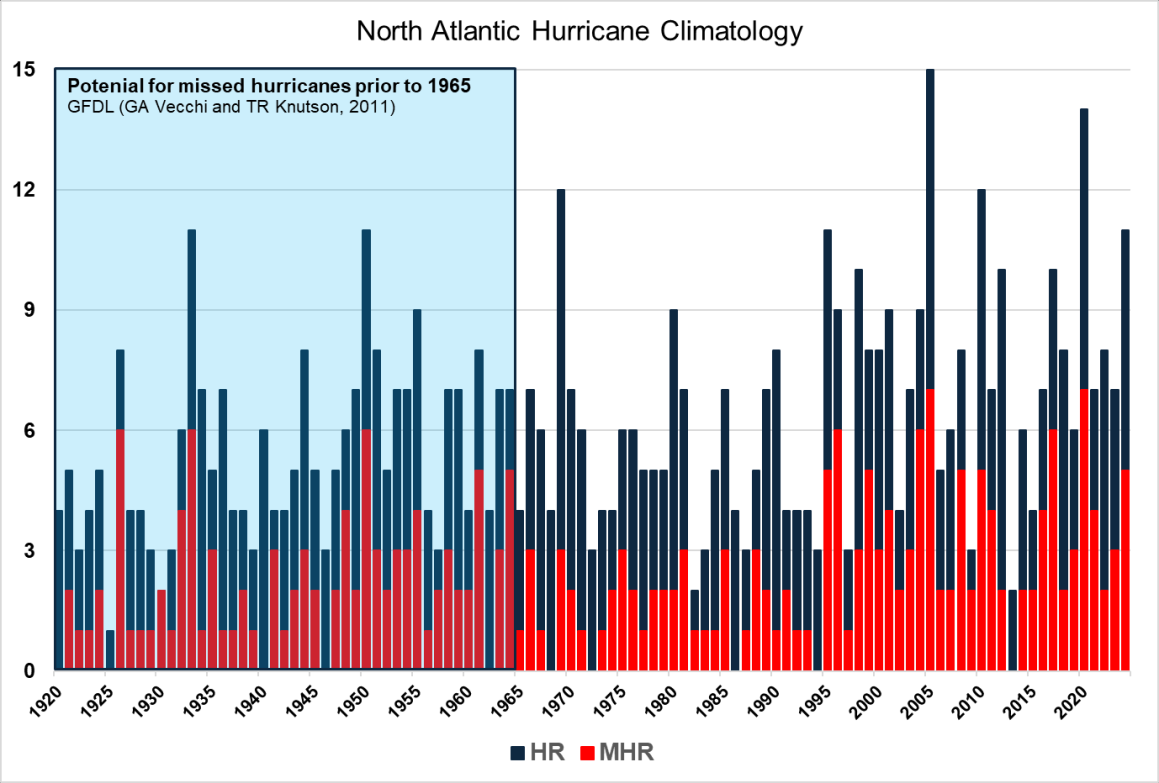
\includegraphics[width=1.0\textwidth]{bilder/bilderKlima-0038.png}\\[1cm]
\end{center}
\caption{Atlantische Häufigkeit von Hurrikans (HR) und schweren Hurrikans (MHR) seit 1920. Quelle: National Hurricane Center (2024)}
\end{figure}

Abbildung 6.2.2 zeigt, dass atlantische Hurrikans stark auf dekadischen und multidekadischen Zeitskalen variieren. Diese Variationen sind primär mit der Atlantischen Multidekadischen Oszillation (AMO) verbunden, die sich in beckenweiten Meeresoberflächentemperatur- und Meeresspiegel-Druckschwankungen manifestiert, die mit großräumigen Ozeanzirkulationsmustern verbunden sind. Die AMO befand sich während 1926-1970 und 1995-heute in ihrer warmen Phase, aber während 1971-1994 in ihrer kühlen Phase. Sie hat ihre größte Auswirkung auf die Anzahl schwerer Hurrikans (Kategorie 3+), die Goldenberg et al. (2001) mit übernormalen SSTs und verringerter vertikaler Scherung in der AMO-Warmphase in Verbindung brachten (siehe auch Bell und Chelliah, 2006; Klotzbach et al., 2018).

Klotzbach et al. (2018) führten eine umfassende Bewertung der auf Land treffenden Hurrikan-Daten für die kontinentalen USA seit 1900 durch. Abbildung 6.2.3 aktualisiert ihre Analyse bis 2024. Während die größten Zahlen landtreffender Hurrikans aus 2004, 2005 und 2020 stammen, gibt es keinen statistisch signifikanten Trend seit 1920. Abbildung 6.2.3 zeigt auch die Zeitreihe für schwere Hurrikan-Landtritte (Kategorie 3-5). Das größte Jahr in der Aufzeichnung ist 2005 mit 4 schweren Hurrikan-Landtritten. Jedoch gab es nach 2005 bis 2016 keine schweren Hurrikans, die die USA trafen - der längste solche Zeitraum seit 1920.

\begin{figure}[H]
\begin{center}
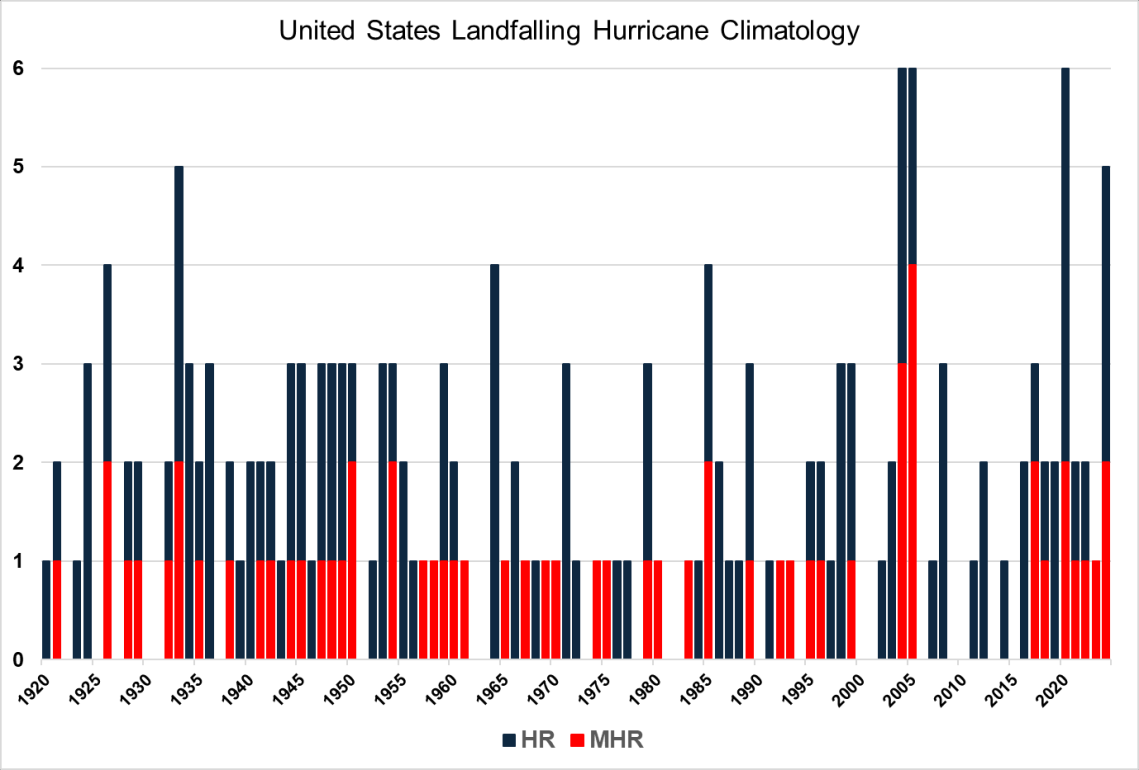
\includegraphics[width=1.0\textwidth]{bilder/bilderKlima-0040.png}\\[1cm]
\end{center}
\caption{US-Landtritt-Häufigkeit von Hurrikans (HR) und schweren Hurrikans (MHR) seit 1920. Quelle: NOAA HRD(a) (2024)}
\end{figure}

Abbildung 6.2.3 zeigt erhebliche zwischenjährliche bis multidekadische Variabilität in der US-Landtritt-Aktivität. Klotzbach et al. (2018) untersuchten, wie die Landtritt-Zahlen mit ENSO (El Niño versus La Niña) und den warmen versus kalten Phasen der Atlantischen Multidekadischen Oszillation (AMO) variieren.

Villarini et al. (2012) liefern eine Analyse der US-Hurrikan-Landtritte zurück bis 1878. Während es möglich ist, dass einige Landtritte im späten 19. Jahrhundert aufgrund dünn besiedelter Regionen an der Golfküste übersehen wurden, ist es bemerkenswert, dass das höchste Jahr in der gesamten Aufzeichnung 1886 ist, mit 7 Hurrikan-Landtritten, als menschliche Einflüsse auf das Klima viel geringer waren als heute.

Tabelle 6.2.1 zeigt die 10 stärksten Hurrikans (plus Gleichstände), die US-Landtritte machten. Von den Hurrikans, die mit anhaltenden Winden größer als 150 mph Landtritte machten, ist nur einer im 21. Jahrhundert aufgetreten.

Tabelle 6.2.1: Stärkste Hurrikans, die an der US-Küste Landtritte machten. Quelle: (NOAA HRD(b), 2024)


\begin{table}[htbp]
  \centering
  
  \label{tab:hurricans}
  \begin{tabular}{
      S[table-format=3.0]
      S[table-format=2.2]
      S[table-format=2.3]
      l
  }
    %\toprule
    {Rang} & {Jahr} & {Landtritt-Wind (MPH)} & {Name} \\
    \midrule
    1  &  1935 & 185 & \glqq Labor Day\grqq{} \\
    2  &  1969 & 175 & Camille \\
    3  &  1992 & 165 &  Andrew\\\
    4  &  2018 & 160 &  Michael \\
    5  &  1856 & 150 & \glqq Last Island\grqq{} \\
    5  &  1886 & 150 & \glqq Indianola\grqq{} \\
    5  &  1919 & 150 & ----- \\
    5  &  1932 & 150 & \glqq Freeport\grqq{} \\
    5  &  2004 & 150 & Charley\\
    5  &  2020 & 150 & Laura \\
    5  &  2021 & 150 & Ida \\
    5  &  2022 & 150 & Ian \\
    \bottomrule
  \end{tabular}
  \caption{Stärkste Hurrikans, die an der US-Küste Landtritte machten. Quelle: (NOAA HRD(b), 2024)}
\end{table}

Zusammenfassend liefern Analysen sowohl globaler als auch regionaler Variabilität und Trends der Hurrikan-Aktivität die Grundlage für die Erkennung von Veränderungen und das Verständnis ihrer Ursachen. Die relativ kurze historische Aufzeichnung der Hurrikan-Aktivität und die noch kürzere Aufzeichnung aus der Satellitenära reichen nicht aus, um zu bewerten, ob die jüngste Hurrikan-Aktivität ungewöhnlich im Verhältnis zur natürlichen Hintergrundvariabilität ist. Atlantische Hurrikan-Prozesse werden erheblich von natürlichen Modi der Ozeanzirkulationsvariabilität im Atlantik beeinflusst, insbesondere der Atlantischen Multidekadischen Oszillation. Während lange hypothetisiert wurde, dass eine steigende globale Meeresoberflächentemperatur eine Zunahme der Hurrikan-Intensität verursachen würde, wird die Identifikation eines signifikanten Trends in den Hurrikan-Daten durch eine kurze Datenaufzeichnung und erhebliche natürliche Variabilität behindert.

Prozessbasiertes Verständnis deutet auch darauf hin, dass Sturmfluten und Niederschläge von Hurrikans mit wärmeren Temperaturen zunehmen sollten. Jedoch verhindern die relativ kleine Anzahl von Hurrikans mit variierenden Landtritt-Orten und die komplexe Dynamik, die mit jedem Sturm verbunden ist, eine aussagekräftige Erkennung von Veränderungen.

\section{Temperaturextreme}
Die AR6-Bewertung konzentrierte sich auf den Zeitraum nach 1950 und berichtete über zunehmende Trends bei Hitzewellen-Häufigkeit und -Intensität. Jedoch stellte NCA4 fest, dass die Hitzewellen-Aktivität in den USA in den 1930er Jahren einen Höhepunkt erreichte (Abbildung 6.3.1).

\begin{quote}
AR6: Es ist praktisch sicher, dass heiße Extreme (einschließlich Hitzewellen) seit den 1950er Jahren häufiger und intensiver geworden sind in den meisten Landregionen, während kalte Extreme (einschließlich Kältewellen) weniger häufig und weniger schwerwiegend geworden sind (SPM, A3.1)

AR6: In Nordamerika gibt es sehr robuste Belege für eine sehr wahrscheinliche Zunahme der Intensität und Häufigkeit heißer Extreme und eine Abnahme der Intensität und Häufigkeit kalter Extreme für den gesamten Kontinent, obwohl es erhebliche räumliche und saisonale Variationen in den Trends gibt. Mindesttemperaturen zeigen eine konsistente Erwärmung über den gesamten Kontinent, während es kontrastierendere Trends bei den jährlichen maximalen Tagestemperaturen in Teilen der USA gibt. (Kapitel 11, S. 1550)

NCA4: Veränderungen bei warmen Extremen sind nuancierter als Veränderungen bei kalten Extremen. Zum Beispiel \textbf{stieg} die wärmste Tagestemperatur des Jahres in einigen Teilen des Westens über das vergangene Jahrhundert, aber es gab \textbf{Abnahmen} in fast allen Orten östlich der Rocky Mountains. Tatsächlich erlebten alle östlichen Regionen eine \textbf{Nettoabnahme}, am deutlichsten im Mittleren Westen (etwa 2,2°F [1,2°C]) und im Südosten (etwa 1,5°F [0,8°C]). (S. 190-191)

NCA4: Seit Mitte der 1960er Jahre gab es nur einen sehr geringen Anstieg der wärmsten Tagestemperatur des Jahres (inmitten großer zwischenjährlicher Variabilität). Hitzewellen (6-Tage-Perioden mit einer Maximaltemperatur über dem 90. Perzentil für 1961–1990) nahmen in der Häufigkeit bis Mitte der 1930er Jahre zu, wurden bis Mitte der 1960er Jahre erheblich seltener und nahmen danach wieder in der Häufigkeit zu. Wie bei warmen Tagestemperaturen \textbf{erreichte die Hitzewellen-Magnitude ein Maximum in den 1930er Jahren. (S. 190-191)}
\end{quote}

\begin{figure}[H]
\begin{center}
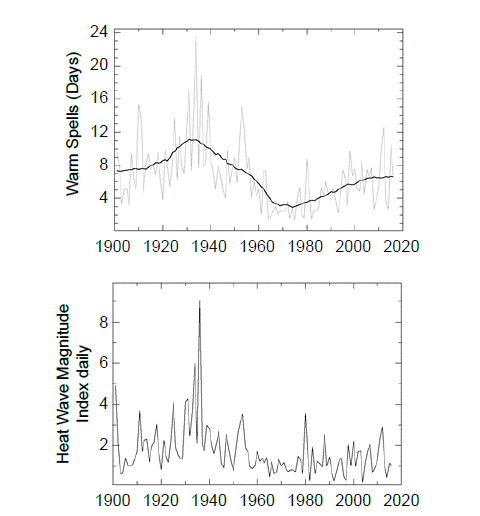
\includegraphics[width=1.0\textwidth]{bilder/bilderKlima-0042.png}\\[1cm]
\end{center}
\caption{US-Hitzewellen seit 1900. Quelle: NCA4 Abbildung 6.4}
\end{figure}

\subsection{Temperaturen in den USA werden weniger extrem}

Tägliche Maximaltemperaturen in der warmen Saison (Tmax, Mai-Sep) und tägliche Minimaltemperaturen in der kalten Saison (Tmin, Dez-Mär) sind verfügbar ab Dezember 1898 (126 Jahre). Der Datensatz besteht aus 1.211 CONUS-Stationen, die als United States Historical Climate Network oder USHCN-Stationen bezeichnet werden (siehe Abbildung 6.3.2; Quinlan et al. 1987, Karl et al. 1990). Diese Stationen wurden von NOAA als diejenigen mit den wenigsten problematischen Problemen mit Lücken, Stationsverlagerungen und Instrumentenänderungen ausgewählt. Wo Lücken noch bestehen, wurden nahegelegene Stationen (verzerrungskorrigiert) zusammengeführt, so dass das mittlere verfügbare Datenvolumen für eine Station 98\% beträgt. Obwohl es sicherlich Fehler im Datensatz gibt, einschließlich ungelöster unechter Erwärmung aufgrund von UHI-Effekten, die besonders Tmin-Aufzeichnungen verzerren, ist dieser Datensatz ausreichend genau für die Bewertung von Trends bei Tmax-Hitzeextremen.

\begin{figure}[H]
\begin{center}
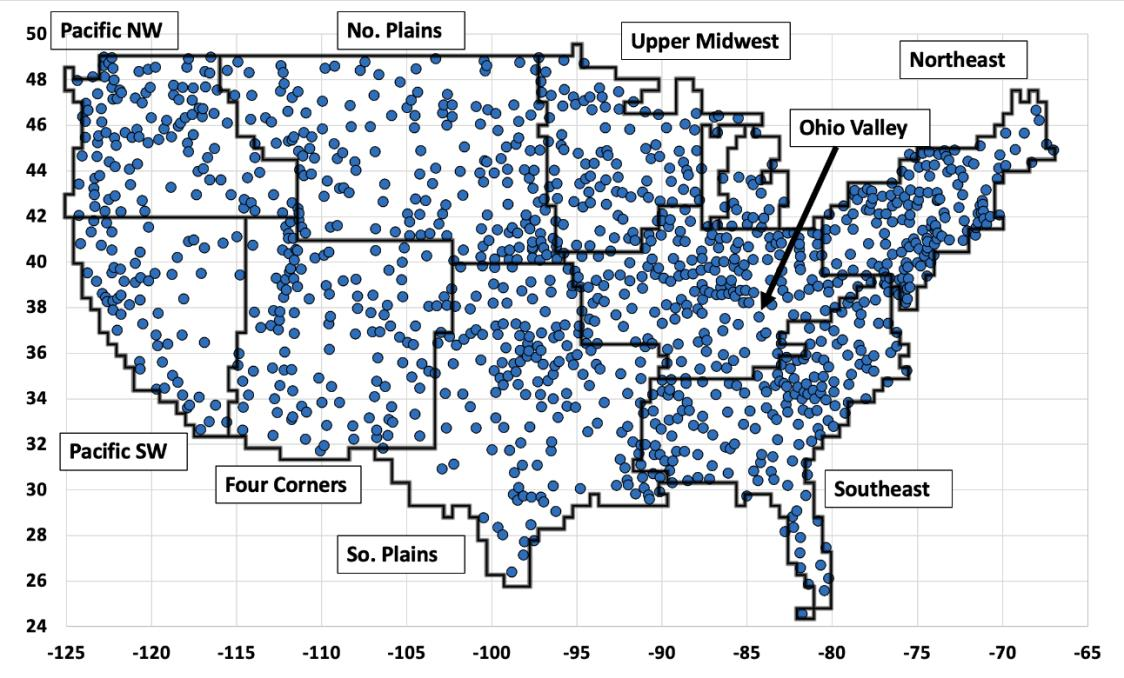
\includegraphics[width=1.0\textwidth]{bilder/bilderKlima-0043.jpg}\\[1cm]
\end{center}
\caption{Standorte der USHCN-Temperaturstationen. Quelle: USHCN.}
\end{figure}

Wir beginnen mit der Frage, ob das Auftreten täglicher Rekord-Hoch- oder Tieftemperaturen sich seit Dezember 1898 verändert hat. Jede warme Saison hat 153 Tage (1. Mai bis 30. Sep) und jede kalte Saison hat 122 Tage (1. Dez bis 31. Mär). Für jede Station und jeden Tag berechneten wir das Jahr, in dem die Rekord-Höchst- (niedrigste) Temperatur auftrat. Mit 126 Jahren Beobachtungen, wenn es keine Temperaturtrends über die Zeit gäbe, wäre die erwartete Anzahl von Rekorden für Tmax 1,21 (=153/126) pro Station pro Jahr und für Tmin 0,96 (=122/126) pro Station pro Jahr.

Abbildung 6.3.3 zeigt die beobachtete Verteilung in der Zeit des Auftretens dieser Extremereignisse. Es gibt ein gemeinsames Merkmal in vielen Metriken der warmsaisonalen Extreme in CONUS - die außergewöhnliche Hitze der 1920er und besonders der 1930er Jahre, mit einem Höhepunkt in 1936. Im Durchschnitt pro Station traten 60 Prozent der Tmax-Rekorde und 59 Prozent der Tmin-Rekorde in der ersten Hälfte des Zeitraums (1899-1961) auf.

\begin{figure}[H]
\begin{center}
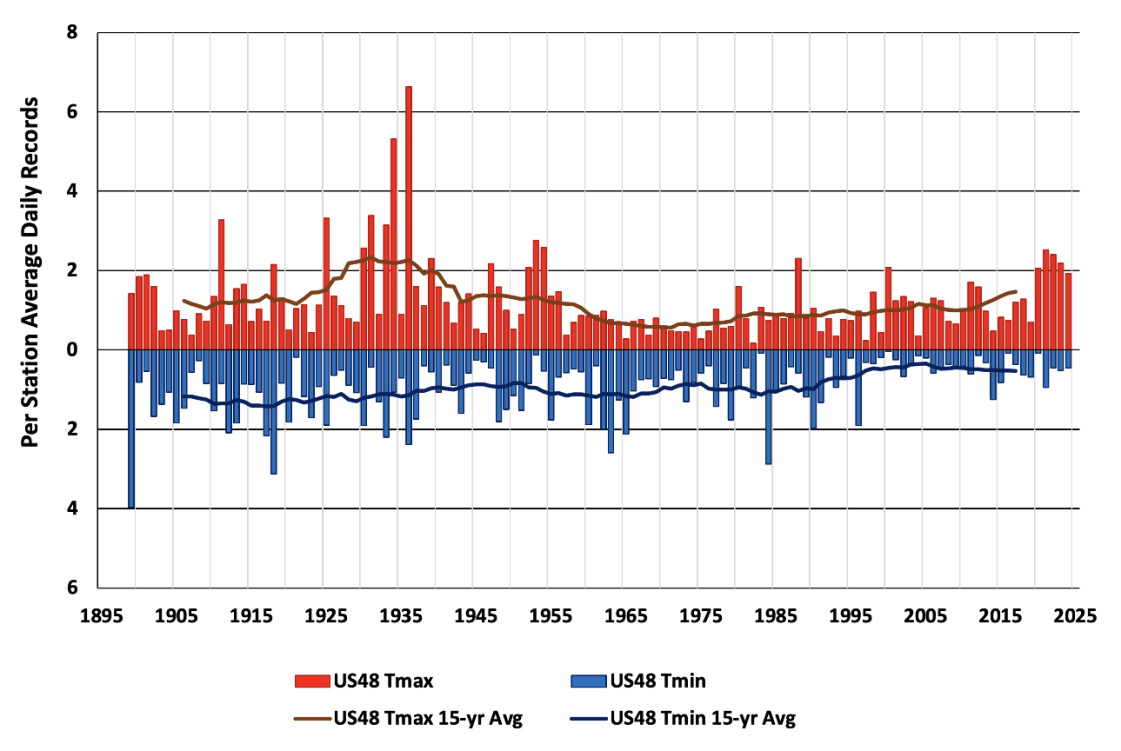
\includegraphics[width=1.0\textwidth]{bilder/bilderKlima-0044.png}\\[1cm]
\end{center}
\caption{Anzahl täglicher Rekord-Hoch- (rot) und Tieftemperaturen (blau) für warme und kalte Saisons in CONUS. Die Linien repräsentieren den 15-jährigen laufenden, zentrierten Durchschnitt. Quelle: 1.211 USHCN-Stationen, nach Bedarf ergänzt, um mindestens 92 Prozent der Beobachtungen in dem 126-jährigen Zeitraum seit Dezember 1898 zu erreichen. US48: zusammenhängende US-Staaten. Tmax: Maximaltemperatur. Tmin: Minimaltemperatur.}
\end{figure}

Auf der kalten Seite steht der Valentinstag-Arktisausbruch im Februar 1899 als das umfassendste Kälteextrem, das CONUS erlebte, mit 1917 an zweiter Stelle. Die Häufigkeit von Kälterekorden ist zurückgegangen, besonders im letzten Viertel des Zeitraums, in dem nur 13 Prozent der extremen Kälteereignisse gemessen wurden. Im Gegensatz dazu wurden 25 Prozent der extremen Tmax-Rekorde im letzten Viertel erreicht, in Übereinstimmung mit statistischen Erwartungen. Diese allgemeinen Merkmale wurden in früheren Bewertungen bemerkt (siehe oben, IPCC AR6, NCA4). Die Kombination der beiden Geschichten zeigt, dass die allgemeine Verringerung der Anzahl sowohl kalter als auch heißer Extreme über das vergangene Jahrhundert auf ein Klima hinweist, das weniger zu Extremen neigt.

Dieses Muster wird auch in Abbildung 6.3.4 gezeigt. Für jede Station und für jedes Jahr wurden die heißesten warmsaisonalen und kältesten kaltsaisonalen Temperaturen berechnet. Dann wurden die Unterschiede zwischen diesen nach Station berechnet und geografisch über alle Stationen gemittelt, was ein jährliches Maß für die erwartete Spanne lokaler Extremtemperaturen für jedes Jahr ergibt. Abbildung 6.3.4 zeigt den 15-jährigen nachlaufenden Durchschnitt dieses Maßes, der über das vergangene Jahrhundert deutlich zurückgegangen ist.

\begin{figure}[H]
\begin{center}
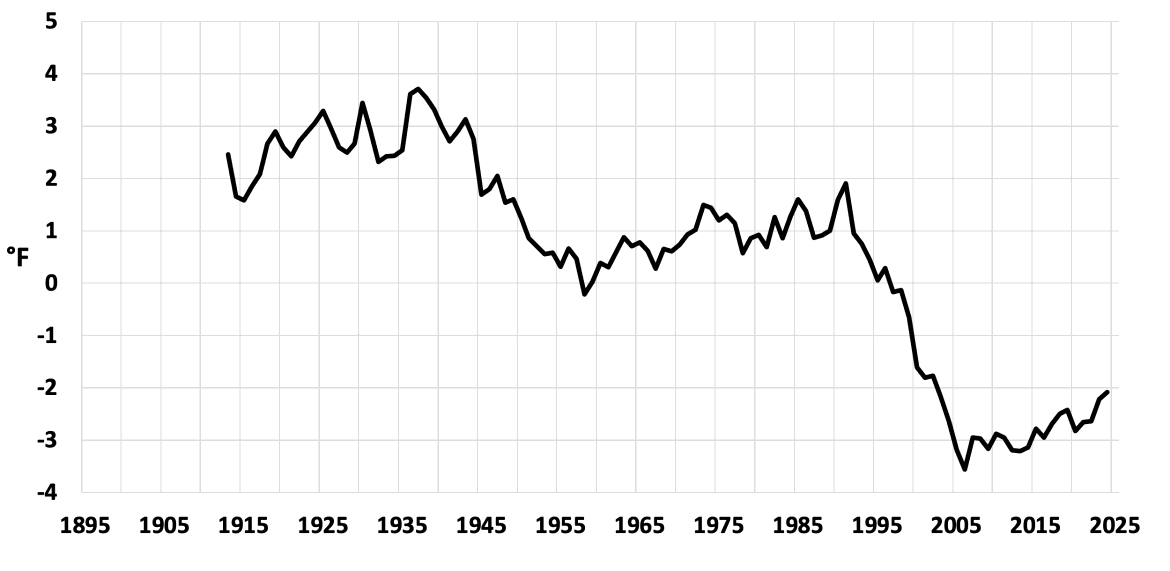
\includegraphics[width=1.0\textwidth]{bilder/bilderKlima-0045.png}\\[1cm]
\end{center}
\caption{15-jähriger nachlaufender Durchschnitt der Differenz jedes Jahres zwischen der heißesten warmsaisonalen Tmax und kältesten kaltsaisonalen Tmin jeder Station relativ zum langfristigen Durchschnitt. Quelle: Autoranalyse von USHCN-Daten.}
\end{figure}

Der durchschnittliche Unterschied für jede Station zwischen der heißesten Sommer-Tmax und kältesten Winter-Tmin ist in den letzten 126 Jahren um etwa \SI{5}{\degree\text{F}} zurückgegangen. Der Rückgang ist hauptsächlich auf wärmere Winter-Tmin zurückzuführen, aber auch ein Rückgang der Sommer-Tmax ist ein Faktor. Der Anstieg von Tmin war stark mit der wachsenden Präsenz von hergestellten Oberflächen um die Wetterstationen in den letzten 100+ Jahren verbunden (der sogenannte städtische Wärmeinseleffekt; Abschnitt 3.3, Karl et al. 1988, Runnals und Oke 2006, und Spencer et al. 2025).

Zusammenfassend zeigen langfristige Aufzeichnungen, während Temperaturextreme regelmäßig in den USA erlebt werden und große Medienaufmerksamkeit anziehen, dass das US-Klima über die Zeit weniger extrem (milder) geworden ist, wenn es durch die Spanne zwischen warmsaisonalen Maxima und kaltsaisonalen Minima gemessen wird.

\subsection{Überschreitungen einer Hitzeschwelle}
Unter der Überschrift \emph{Das Risiko von Temperaturextremen verändert sich} bemerkt der neueste US National Climate Assessment Report (NCA5) den Anstieg einer Schwellenwert-Metrik der Anzahl von Tagen bei oder über \SI{95}{\degree\text{F}} und stellt fest:
\begin{quote}
Die westlichen USA wurden seit den 1980er Jahren besonders von extremer Hitze betroffen..., mit einem größeren Anstieg von Tagen über \SI{95}{\degree\text{F}}, wie erwartet angesichts der größeren Erwärmung in dieser Region relativ zu den östlichen USA. Mehrere große Hitzewellen haben die USA seit 2018 betroffen, einschließlich eines rekordverschmetternden Ereignisses im pazifischen Nordwesten in 2021.
\end{quote}

Verändern sich die Auftreten von \SI{95}{\degree\text{F}}-Tagen? In einem so vielfältigen Klima wie dem von CONUS können Schwellenwert-Statistiken irreführend sein. Eine Region mit vielen Stationen, die nahe \SI{95}{\degree\text{F}} Tmax-Durchschnittstemperaturen im Sommer haben, könnte große Schwankungen in der Metrik sehen, wenn nur kleine Änderungen in der Durchschnittstemperatur auftreten. Anderswo, mit Stationen, die entweder selten oder praktisch immer \SI{95}{\degree\text{F}} Tmax-Temperaturen erreichen, wird eine kleine Änderung nicht viel Auswirkung auf die Ergebnisse haben.

\begin{figure}[H]
\begin{center}
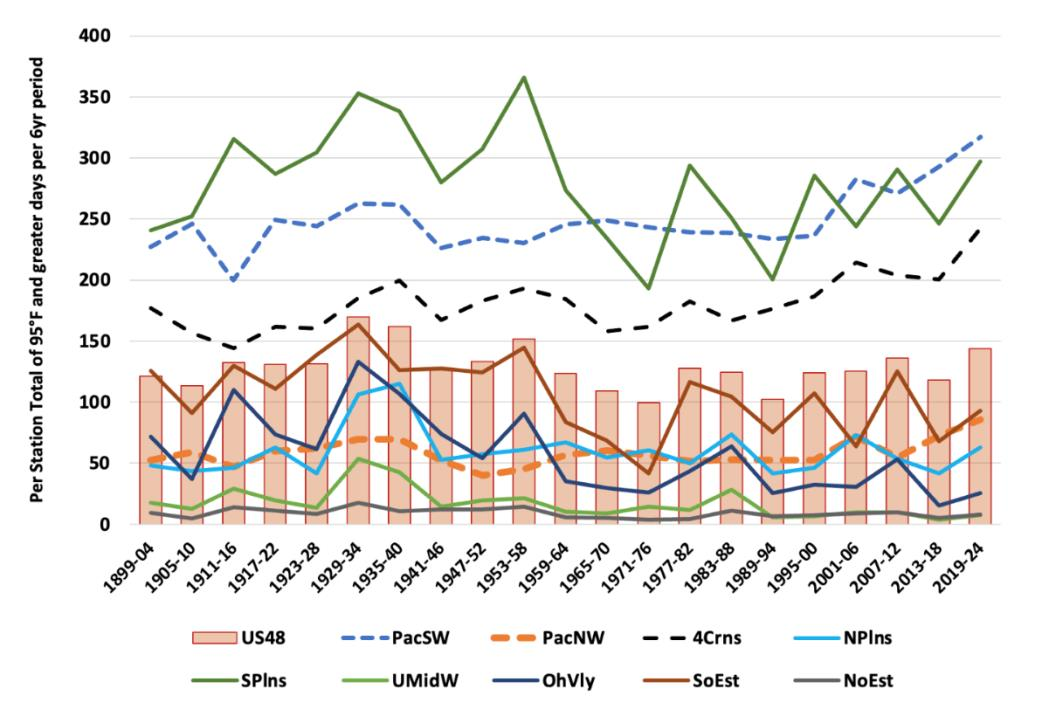
\includegraphics[width=1.0\textwidth]{bilder/bilderKlima-0046.jpg}\\[1cm]
\end{center}
\caption{Gesamtanzahl von Tagen $\geq$ \SI{95}{\degree\text{F}} in 6-jährigen Perioden, US 48 (Balken) und Regionen (Linien). Eine 6-Jahres-Periode wird verwendet, da dies die 126-jährige Aufzeichnung gleichmäßig teilt. Ergebnisse sind robust bei Verwendung von Perioden von 2 bis 11 Tagen. US48: zusammenhängende US-Staaten. Siehe Abbildung 6.3.2 für Regionsnamen. Quelle: Autoranalyse von USHCN-Daten.}
\end{figure}

In den letzten 126 Jahren erlebte die durchschnittliche CONUS-Station 129 Tage, die 95°F pro 6-Jahres-Periode überschritten, aber die regionalen Werte reichen von 278 in den Southern Plains bis 9 im Nordosten. Daher müssen solche Schwellenwert-Analysen mit Vorsicht interpretiert werden. Abbildung 6.3.5 zeigt, dass nur drei der neun Regionen, alle im Westen, aufwärts gerichtete Trends bei der Anzahl von 95°F oder heißeren Tagen erlebt haben (gestrichelte Linien). CONUS als Ganzes hat das nicht, und die anderen sechs Regionen haben Rückgänge erlebt.

Die pazifische Nordwest-Hitzewelle von 2021, die im NCA5-Zitat erwähnt wird, wird in Abschnitt 8.6.1 näher untersucht. Die Evidenz zeigt, dass es ein einzelnes, beispielloses Ereignis in der Aufzeichnung war, nicht Teil eines Musters zunehmender extremer Hitze. Zum Beispiel war die 5-Tage-Durchschnitts-Troposphären-Gitterpunkt-Temperaturanomalie über dem pazifischen Nordwesten während dieses Ereignisses +10,8°C, die extremste Sommer-Anomalie der nördlichen Hemisphäre an Gitterpunkten in den 46 Jahren aus über 4 Millionen Gitterwerten. Im Gegensatz dazu war die globale Temperaturanomalie während dieser Zeit praktisch null (+0,03°C, Mass et al. 2024).

\subsection{Hitzewellen}
Hitzewellen (aufeinanderfolgende Tage, die eine extreme Schwelle überschreiten) haben eine größere gesellschaftliche Auswirkung als eine einzelne tägliche Rekordtemperatur. Wir messen "Hitzewellen-Tage" hier als die Anzahl aller Tage im Mai-September jedes Jahres, die das 90. Perzentil für diesen Tag überschreiten und die innerhalb einer Periode von mindestens sechs aufeinanderfolgenden Tagen liegen. Dies entspricht der in NCA4 verwendeten Methode, außer dass der Referenzzeitraum hier die gesamte Aufzeichnung 1899-2024 ist, während NCA4 den Referenzzeitraum auf 1961-1990 kürzte, was ein kühles Intervall war. (Das unten gezeigte Ergebnismuster hängt nicht von der Wahl des Referenzzeitraums ab.) Diese Kürzung verstärkt positive Ergebnisse (Tage, die das 90. Perzentil überschreiten) in Jahren, die wärmer als der Referenzzeitraum sind, besonders ab 1960 bis zur Gegenwart (siehe Abbildung 6.3.6 und Diskussion unten).

\begin{figure}[H]
\begin{center}
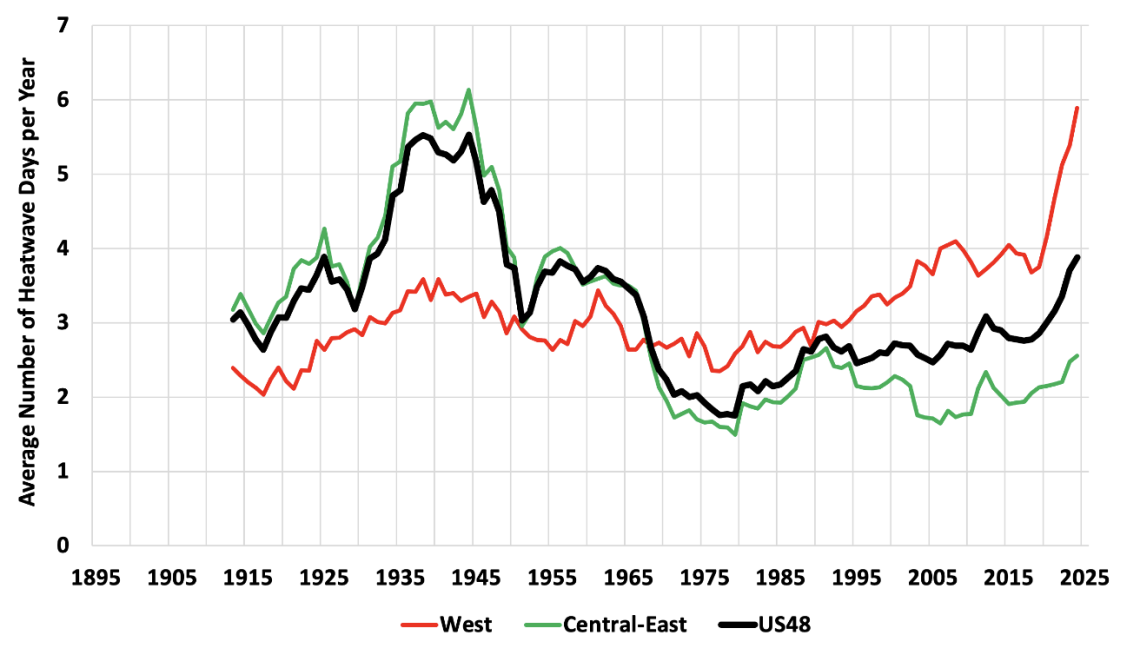
\includegraphics[width=1.0\textwidth]{bilder/bilderKlima-0047.png}\\[1cm]
\end{center}
\caption{15-jähriger nachlaufender Durchschnitt der Anzahl von Hitzewellen-Tagen pro Jahr pro Station in CONUS (schwarze Linie) und zwei Regionen: Westen (rot), Zentral-Osten (grün).}
\end{figure}

Abbildung 6.3.6 zeigt, dass es regionale Variationen in der Hitzewellen-Aktivität gibt. Die übermäßige Hitze der ersten Hälfte des 20. Jahrhunderts trat primär in den östlichen zwei Dritteln der Nation auf, während der Westen einen jüngsten Anstieg von Hitzewellen-Tagen gesehen hat (NCA5). Dies zeigt, dass die Hintergrund-Warmsaison-Zirkulation Hitzewellen in den östlichen Teilen des Landes in der ersten Hälfte des 20. Jahrhunderts begünstigte, aber im 21. Jahrhundert haben die Muster Hitzewellen im Westen begünstigt. Für CONUS als Ganzes sind Hitzewellen heute nicht häufiger als vor einem Jahrhundert, konsistent mit dem oberen Panel unserer Abbildung 6.4.1 aus NCA4.

Diese Metrik variiert erheblich mit der Region. Die vier nördlichen Regionen (Pacific NW, Northern Plains, Upper Midwest und Northeast) erleben im Durchschnitt 15 bis 27 Hitzewellen-Tage pro 15-Jahres-Periode. Im Gegensatz dazu sehen die fünf südlichen Regionen (Pacific Southwest, 4-Corners, Southern Plains, Ohio Valley und Southeast) 37 bis 54 solche Tage, im Wesentlichen doppelt so viele. Dies deutet darauf hin, dass das Sommer-Zirkulationsmuster in den südlichen Regionen anfälliger für stationäre Ereignisse ist, während transiente Systeme in den nördlichen Regionen häufiger sind und daher diese potenziell längeren Ereignisse verkürzen.

Die Analyse von Hitzewellen ist ein Beispiel dafür, warum es wichtig ist, vollständige Datensätze und angemessene Metriken zu betrachten. NCA5 leitet Leser zur Website https://www.globalchange.gov/indicators/heat-waves (USGCRP 2023), um eine Abbildung zu sehen, die die Anzahl städtischer Hitzewellen nach Jahrzehnten ab den 1960er Jahren zeigt, die wir als Abbildung 6.3.7 reproduzieren.

\begin{figure}[H]
\begin{center}
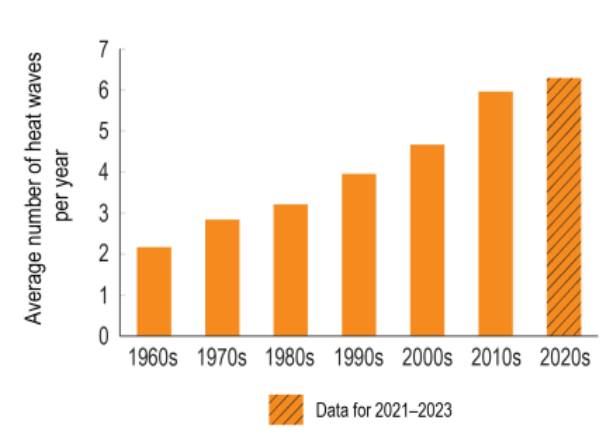
\includegraphics[width=1.0\textwidth]{bilder/bilderKlima-0048.png}\\[1cm]
\end{center}
\caption{Durchschnittliche Anzahl städtischer Hitzewellen pro Jahr für 50 große US-Metropolregionen, eine irreführende Metrik aus Gründen, die im Text erklärt werden. Von \url{https://www.globalchange.gov/indicators/heat-waves} (aufgerufen am 22. Mai 2025).}
\end{figure}

Die Abbildung zeigt einen monotonen Anstieg in jedem Jahrzehnt von zwei Auftreten pro Jahr in den 1960er Jahren auf sechs in den 2020er Jahren. Die verwendete Definition einer Hitzewelle ist ein ungewöhnliches, aber praktisches Maß menschlichen Unbehagens - eine Periode von mindestens 2 aufeinanderfolgenden Tagen, wenn die minimale scheinbare Temperatur (Kombination von Temperatur und Feuchtigkeit) das 85. Perzentil überschreitet. Beachten Sie auch, dass der Datensatz auf die 50 größten US-Städte beschränkt ist.

Angesichts der ungewöhnlichen Hitzewellen-Definition und des städtischen Fokus sind diese steigenden Werte seit 1960, die in USGCRP (2023) präsentiert werden, nicht informativ über langfristige Trends oder den Einfluss von THG-Emissionen aus mindestens zwei Gründen. Erstens, wie in Abbildungen 6.3.1 und 6.3.6 gezeigt, waren die 1960er Jahre das kälteste Jahrzehnt und die 1970er Jahre das zweitkälteste Jahrzehnt seit den 1910er Jahren, sodass dieses Startdatum die Zeitreihe darauf vorkonditioniert, Anstiege zu zeigen. Zweitens ist die Urbanisierung nach 1960 in diesen Städten ein Hauptfaktor für den Anstieg von Tmin relativ zu ko-lokalisierten Tmax und relativ zu Tmin an nahegelegenen ländlichen Stationen (Karl et al. 1988, Runnals und Oke 2006, Christy et al. 2009, McNider et al. 2012). Dies schmälert nicht den realen Anstieg der nächtlichen Temperaturen in großen US-Städten und die gesellschaftlichen Auswirkungen, die mit diesen Änderungen verbunden sind. Jedoch bemerken wir aus verschiedenen Gründen, dass Sommer-Tmax (besonders in ländlichen Gebieten) eine bessere Metrik für die Erkennung von Änderungen in Hitzewellen ist, die von Änderungen im Hintergrundklima beeinflusst werden, zum Beispiel aufgrund steigender THGs (Christy et al. 2009). Für CONUS als Ganzes deutet die Evidenz in diesem Abschnitt darauf hin, dass THG-Emissionen wenig bis keine Auswirkung auf Hitzewellen vor dem Hintergrund von Urbanisierung und natürlicher Klimavariabilität hatten. Unabhängig von der ultimativen Ursache regionaler Trends haben Hitzewellen wichtige Auswirkungen auf die Gesellschaft, die angegangen werden müssen, wie wir in Kapitel 10 diskutieren.

\begin{fullbox}{BOX: Gefahren kurzer Datenaufzeichnungen}
% --- Oberer (fließender) Teil: darf über mehrere Seiten laufen ---
San Francisco bietet eine gute Fallstudie der Begrenzung der Verwendung kurzer historischer Stichproben zur Charakterisierung natürlicher Variabilität von Extremereignissen. Angenommen, wir verwenden eine 130-jährige Stichprobe täglicher San Francisco-Niederschläge von 1895 bis 2024 und wir suchen nach 3-Tage-, 5-Tage-, 14-Tage- und 30-Tage-Niederschlagsrekorden. Die Ergebnisse sind wie in Tabelle 6.2 gezeigt.

\begin{center} 
  \begin{tabular}{
       l
       S[table-format=2.2]
       S[table-format=4.0]
   }
  \toprule
  \multicolumn{1}{l}{Ereignis} & 
  \multicolumn{1}{c}{Rekord (Zoll)} & 
  \multicolumn{1}{c}{Jahr} \\
  \midrule
     3-Tage   &  6.94 & 2023 \\
     5-Tage   &  8.55 & 2023 \\
    14-Tage   & 12.62 & 2023 \\
    30-Tage   & 18.93 & 1998 \\
  \bottomrule
  \end{tabular}
  \captionof{table}{Extreme Niederschlagsrekorde, San Francisco, 1895–2024.}
  \label{tab:box2table1}
\end{center}

Die Rekorde gruppieren sich alle in den jüngeren Jahren. 2023 scheint ein außergewöhnliches Jahr zu sein, und da es nahe dem Ende der Stichprobe liegt, könnte es darauf hindeuten, dass das Klima in einen gefährlicheren Zustand gewechselt ist, vielleicht aufgrund menschlicher Einflüsse. [Hinweis: "2023" zeigt an, dass das Ereignis im Wasserjahr von Aug 2022 bis Juli 2023 auftrat.]

Aber das Bild ist sehr anders, wenn wir eine Stichprobe verwenden, die 45 Jahre früher beginnt, in 1850. Tabelle 6.3 zeigt, dass die rekordschaffenden Ereignisse alle in den 1860er Jahren passierten. Außerdem ist 2023 jetzt nicht einmal an zweiter Stelle, sondern fällt auf den 3. oder 4. Platz. Und ein Vergleich der Rekorde der beiden Tabellen zeigt, dass die extremen Niederschlagsereignisse in 1862 und 1867 erheblich mehr Niederschlag beinhalteten als die Ereignisse von 1998 und 2023, mit 14- und 30-Tage-Summen etwa 50 Prozent höher.

\noindent
\begin{minipage}{\textwidth}
\begin{center}
  \begin{tabular}{
        l
        S[table-format=2.2]
        S[table-format=4.0]
        >{\centering\arraybackslash}p{5.5cm}
  }
    \toprule
    \multicolumn{1}{l}{Ereignis} &
    \multicolumn{1}{c}{Rekord (Zoll)} &
    \multicolumn{1}{c}{Jahr} &
    \makecell{Rang des 130-Jahresextrems\\ aus Tabelle 6.2} \\
    \midrule
    3-Tage   &  8.85 & 1867 & 3 \\
    5-Tage   &  9.80 & 1867 & 3 \\
    14-Tage  & 19.05 & 1862 & 4 \\
    30-Tage  & 28.25 & 1862 & 2 \\
    \bottomrule
  \end{tabular}
  \captionof{table}{Extreme Niederschlagsrekorde, San Francisco, 1850–2024.}
  \label{tab:box2tab2}
\end{center}
\end{minipage}


% --- Unterer Teil: wird ans Boxende (letzte Seite) gesetzt ---
Die Spanne natürlicher Variabilität wird noch bemerkenswerter, wenn paläoklimatische Evidenz untersucht wird. Porter et al. (2011) entdeckten, dass in den letzten 1.800 Jahren mindestens sechs Megastürme intensiver waren als der verheerende 1861-62 ARkStorm, der die Region traf.

Dieses Beispiel illustriert die Begrenzungen der Verwendung relativ kurzer Klimazeiträume (~130 Jahre) zur Bewertung des Charakters und der Spanne natürlicher Variabilität im Allgemeinen und von Extremereignissen im Besonderen. Eine genaue Darstellung der vollen Spanne natürlicher Variabilität ist notwendig für jede Attributionsanalyse (Abschnitt 8.6). Infrastrukturplaner, Notfallmanagement-Institutionen und Attributionswissenschaftler würden die erhebliche Falschdarstellung der Magnitude eines zukünftigen Extrems verstehen, wenn sie nur auf den letzten 130 Jahren basiert. In diesem Fall liefert eine einzelne Zeitstichprobe von 130 Jahren eine Unterschätzung des Extremwertes um bis zu 50 Prozent, die bestimmt wird, wenn nur 45 weitere Jahre von Beobachtungen hinzugefügt werden. Verglichen mit paläoklimatischer Evidenz auf Jahrtausend-Skala würde eine noch größere Unterschätzung auftreten. Eine wichtige Lehre ist, dass das Klima große Überraschungen von sich aus liefern kann, sogar ohne menschliche Einflüsse.
\end{fullbox}

\section{Extreme Niederschläge}
AR6 bewertete, dass eine Zunahme starker Niederschläge in Daten ab den 1950er Jahren beobachtet wurde.
\begin{quote}
AR6: Die Häufigkeit und Intensität starker Niederschlagsereignisse haben seit den 1950er Jahren über den meisten Landgebieten zugenommen, für die Beobachtungsdaten für Trendanalysen ausreichend sind (hohes Vertrauen). (SPM A3.2)

AR6: In Nordamerika gibt es robuste Evidenz, dass die Magnitude und Intensität extremer Niederschläge seit den 1950er Jahren sehr wahrscheinlich zugenommen hat. Sowohl [Ein-Tages-Maxima] als auch [5-Tages-Maxima] haben in Nordamerika während 1950-2018 signifikant zugenommen. (Kapitel 11, S. 1560)
\end{quote}

Die US National Climate Assessments (NCA4, NCA5) haben eine Zunahme des Auftretens der stärksten Niederschlagsereignisse (auf verschiedene Weise definiert) primär in der östlichen Hälfte von CONUS hervorgehoben, besonders im Nordosten, wenn die Analyse entweder 1901 oder 1958 beginnt. Interessanterweise zeigen die regionalen Variationen, dass die größten Zunahmen extremer Niederschlagsereignisse im Nordosten und die kleinsten im Westen auftreten, ein Muster entgegengesetzt zu den Änderungen bei Temperaturextremen (Abbildung 6.3.6).

McKitrick und Christy (2019) untersuchten langfristige und konsistente Stationsbeobachtungen extremer täglicher Niederschläge, um einige dieser NCA-Behauptungen für den Südosten und die Westküste zu testen, unter Verwendung eines Trendmodells mit einem nichtparametrischen Varianzschätzer, der robust gegen die komplexen Autokorrelationseigenschaften von Niederschlagsdaten ist. Als die Zeitreihen zeitlich zurück verlängert wurden (in einigen Fällen bis 1872) oder später begannen (1978), gab es keine signifikanten Trends für beide Regionen.

Diese Befunde wurden für diesen Bericht aktualisiert (McKitrick und Christy 2025) mit ähnlich konstruierten Beobachtungen von 29 Stationen an der pazifischen CONUS-Küste (1893ff von San Diego CA bis Blaine WA) und 24 Stationen im feuchten Südosten (1872ff von Austin TX bis Washington DC), sowie der Hinzufügung von 27 Stationen im Nordosten (1888ff von Buffalo NY bis Eastport ME). Die Standorte sind in Abbildung 6.4.1 gezeigt. Die Stationen wurden basierend auf der Verfügbarkeit langfristiger hochwertiger Aufzeichnungen ausgewählt. Die Regionen sind jeweils mit wichtigen Merkmalen extremen Niederschlagsverhaltens verbunden: die Pazifikküste ist mit landtreffenden atmosphärischen Flüssen verbunden, für die AR6 Evidenz zunehmender Aktivität seit 1948 mit weiteren Zunahmen anführt, die erwartet werden, während sich die Welt erwärmt (AR6 8.3.2.8.2); der NCA-Bericht zeigt, dass der Nordosten die größte Zunahme extremer Ereignisse erlebt hat, und der Südosten ist ebenfalls ein Ort, der in den NCAs als mit zunehmenden extremen Ereignissen vermerkt wird.

Die Ergebnisse der Anwendung der Analyse von McKitrick und Christy (2019) waren wie folgt für jede Region, gefolgt von weiterer Erklärung.
Abbildung 6.4.1: Standorte der Niederschlagsüberwachungsstationen, die in diesem Bericht verwendet werden. Orange: Pazifikküste. Blau: Nordosten. Grün: Südosten. Daten von McKitrick und Christy (2025).


\textbf{Starke Niederschlagsereignisse an der Pazifikküste}
\begin{itemize}
\item Der durchschnittliche Niederschlagstrend ist statistisch signifikant (abwärts) in Astoria OR; anderswo nicht signifikant. 
\item Der Trend in der Niederschlagsvarianz ist positiv und signifikant in Big Sur CA; anderswo nicht signifikant. 
\item Der Trend im täglichen maximalen Niederschlag ist positiv und signifikant in Aberdeen WA und Big Sur CA und negativ und signifikant in Newport OR (anderswo nicht signifikant). 
\item Gemittelt über alle Stationen in der Region ist keiner dieser drei Trendparameter statistisch signifikant.  
\end{itemize}

Die Pazifikküste erhält beträchtliche Niederschläge von Atmospheric River (AR) Ereignissen, die oft mehr als ein oder zwei Tage dauern (z.B., Gershunov et al. 2017, Pan et al. 2024). Die schlimmste Serie solcher Ereignisse in der jüngeren Geschichte war der sogenannte ARkStorm, der im Dezember 1861 und Januar 1862 auftrat; er schüttete fast 10 Fuß Regen in Teilen Kaliforniens aus und tauchte das gesamte Central Valley wochenlang unter bis zu 15 Fuß Wasser (Brewer 1930, Null und Hulbert 2007). Zusätzlich hat paläoklimatische Forschung sechs Megastürme gefunden, die schwerwiegender waren als 1861–1862 in Kalifornien während der letzten 1800 Jahre, auftretend in Intervallen von etwa 300 Jahren (Porter et al. 2011).

\begin{figure}[H]
\begin{center}
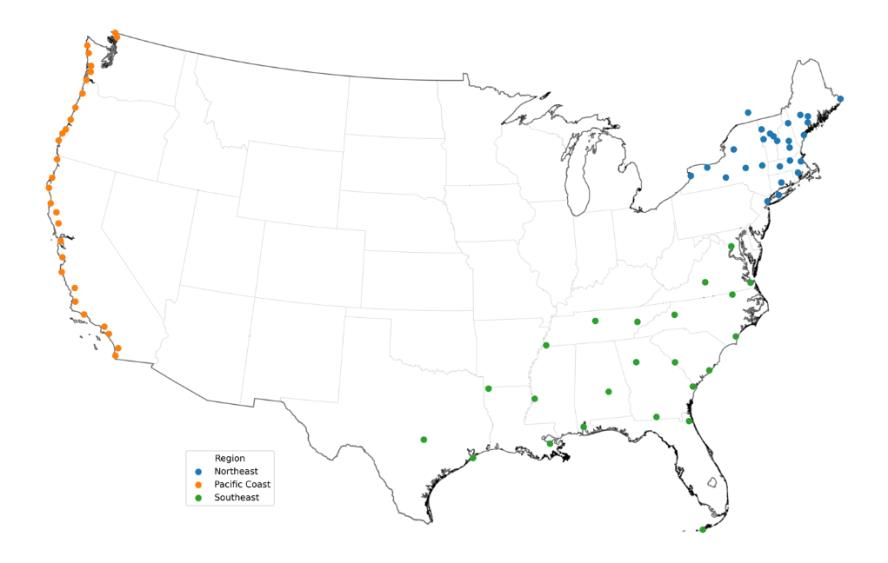
\includegraphics[width=1.0\textwidth]{bilder/bilderKlima-0055.jpg}\\[1cm]
\end{center}
\caption{Standorte der in diesem Bericht verwendeten Niederschlagsmessstationen.
Orange: Pazifikküste. Blau: Nordosten. Grün: Südosten. Daten von McKitrick und
Christy (2025).}
\end{figure}

Wir untersuchen Auftreten von 5-Tage-Wassermassen wie folgt. Die Pazifikküste als Beispiel nehmend, enthält eine 130-jährige Spanne 26 5-Jahres-Intervalle. An jedem Standort berechneten wir die 5-Tage-Niederschlagssummen das ganze Jahr über und wählten die 26 höchsten Werte über die Stichprobe aus. Ein einzelnes Jahr könnte mehr als eines der 26 schwersten haben. Jedes davon kann als 1-in-5yr-Ereignis betrachtet werden. Wenn es keine Trends im Niederschlag gibt, dann sollte die Gesamtzahl dieser Ereignisse über alle Stationen gleichmäßig über die Jahre verteilt sein. In Abb. 6.4.2 zeigen wir die Verteilung in der Zeit dieser Ereignisse für die Pazifikküste. Die Wassermassen, die mit dem massiven 1997-98 El Niño-Ereignis verbunden sind, sind leicht erkennbar. Während unregelmäßig, wie typisch für solche Niederschlagsmetriken, gibt es keine Anzeichen einer Tendenz, über die Zeit häufiger zu werden.

\begin{figure}[H]
\begin{center}
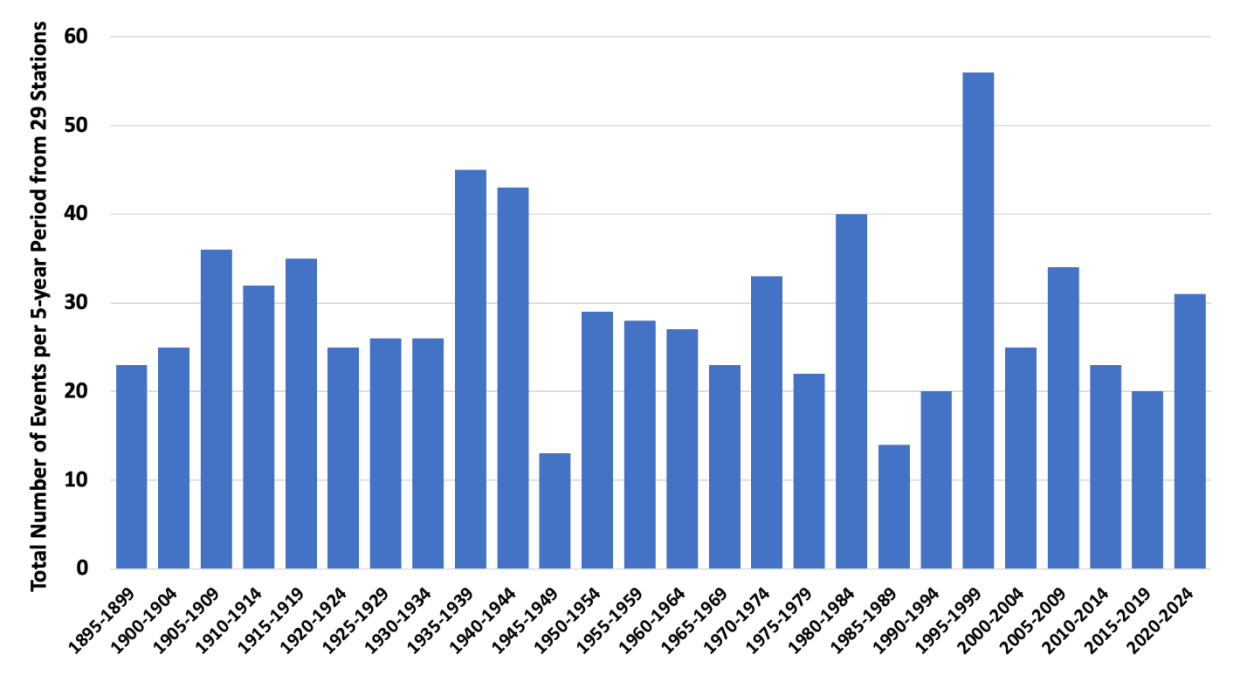
\includegraphics[width=0.9\textwidth]{bilder/bilderKlima-0056.png}\\[1cm]
\end{center}
\caption{Die Zeitverteilung in 5-Jahres-Perioden der 26 schwersten (1-in-5 yr) Auftreten für 29 Stationen an der Pazifikküste.}
\end{figure}
\begin{figure}[H]
\begin{center}
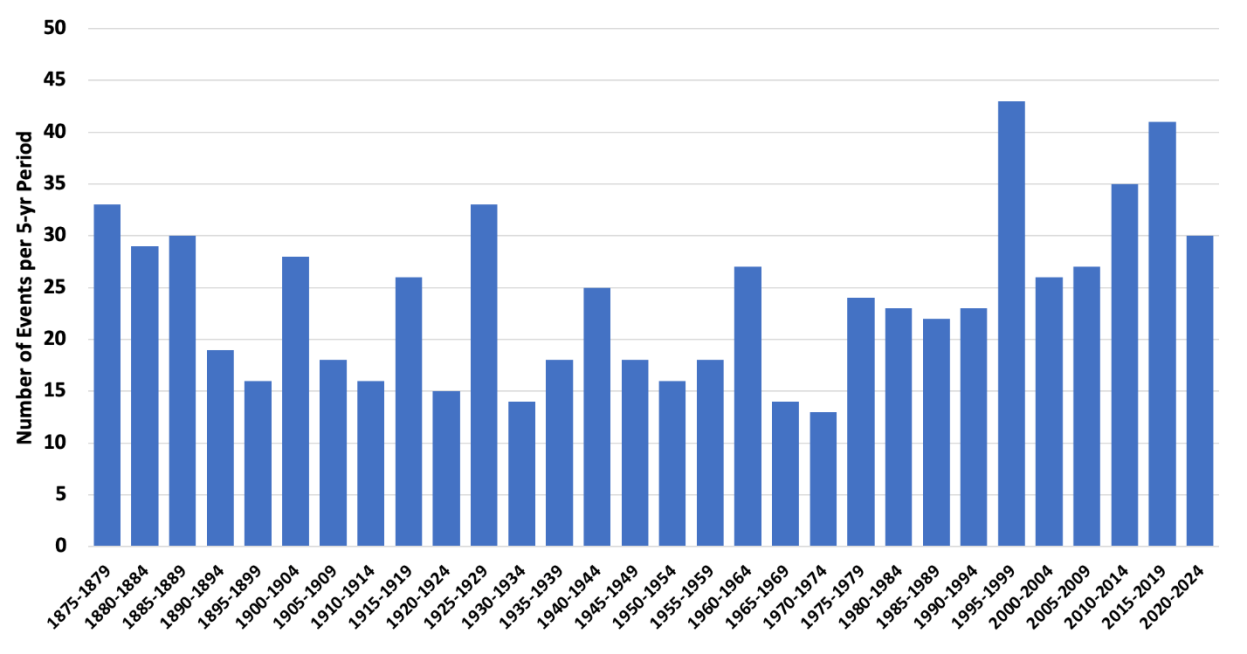
\includegraphics[width=0.9\textwidth]{bilder/bilderKlima-0057.png}\\[1cm]
\end{center}
\caption{Wie in Abb. 6.4.2, jedoch für die 30 schwersten Ereignisse (1-in-5-Jahre) für 24 Stationen im feuchten
Südosten von Austin, Texas, bis Washington, D.C., in 5-Jahres-Intervallen für den Zeitraum 1875–2024.}
\end{figure}

\textbf{Starke Niederschlagsereignisse im Südosten}
\begin{itemize}
\item Der Trend im durchschnittlichen Niederschlag ist positiv und statistisch signifikant in Mobile AL und Quitman GA, aber anderswo nicht signifikant. 
\item Der Trend in der Niederschlagsvarianz ist positiv und signifikant in Mobile AL, aber anderswo nicht signifikant.
\item Der Trend im täglichen maximalen Niederschlag ist positiv und signifikant in Vicksburg MS und Norfolk VA, aber anderswo nicht signifikant.
\item Gemittelt über alle Stationen in der Region ist keiner dieser drei Trendparameter statistisch signifikant. 
\end{itemize}

Abbildung 6.4.3 ist analog zu Abbildung 6.4.2 für die letzten 150 Jahre in der feuchten Südost-Zone. Das zeitliche Muster der 5-Tage-Summen der 1-in-5yr schweren Ereignisse ist allgemein unauffällig, obwohl eine Häufung höherer Werte von 1995 bis 2019 erscheint. Die Zunahme in diesen Jahren ist größtenteils auf die 4 nordöstlichsten Stationen von Wilmington NC, Weldon NC, Washington DC und Norfolk VA zurückzuführen. Dies bestätigt das in NCA4 und NCA5 angedeutete Muster -- eine zunehmende Häufigkeit schwerer Ereignisse aufgrund einer zeitlichen Häufung tropischer Stürme von Ost-NC bis Maine, die unten diskutiert wird. Ansonsten zeigen die verbleibenden 20 Stationen eine unauffällige zeitliche Verteilung schwerer Ereignisse.

\textbf{Starke Niederschlagsereignisse im Nordosten}
\begin{itemize}
\item Der Trend im durchschnittlichen Niederschlag ist positiv und statistisch signifikant in 12 von 27 Standorten und auch im regionalen Durchschnitt. 
\item Der Trend in der Niederschlagsvarianz ist positiv und signifikant in Portland ME, Albany NY, Buffalo NY und Eastport ME, aber anderswo nicht signifikant. 
\item Der Trend im täglichen maximalen Niederschlag ist positiv und signifikant in Portland ME, Gardiner ME und Eastport ME, aber anderswo nicht signifikant. 
\item Wenn über alle Stationen in der Region gemittelt, gibt es keinen statistisch signifikanten Trend in entweder der Niederschlagsvarianz oder dem Maximum. 
\end{itemize}




Abb. 6.4.4 ist analog zu Abbildung 6.4.2 für die letzten 135 Jahre in 27 Stationen im Nordosten (einschließlich Montreal Kanada). Wir verwenden hier 3-Tage-Summen, da dies die größten zeitlichen Variationen in der Zeit produzierte. In dieser Region treten 77 Prozent der Ereignisse während Juni bis Oktober auf und werden von Einbrüchen von Hurrikans, tropischen Stürmen oder tropischen Stürmen dominiert, die zu außertropischen Systemen übergehen. Laut NCA4 und NCA5 erlebte diese Region die größten Zunahmen extremer Ereignisse, sodass sie eine nähere Untersuchung verdient.

Es gibt eine bemerkenswerte Häufung extremer Ereignisse von 1995 bis 2014. Howarth et al. (2019) untersuchten eine ähnliche Region wie in Abb. 6.4.4, die PA und NJ einschließt, und berichteten signifikante Unterschiede in verschiedenen Niederschlagsextremen zwischen zwei 18-Jahres-Perioden, 1979-96 und 1997-2014. Das schloss eine 317-prozentige Zunahme von 24-Stunden-Ereignissen ein, die 6 Zoll überschreiten, während wir eine 58-prozentige Zunahme über dieselben Jahre finden. Jedoch zeigt Abbildung 6.4.4, dass die Häufigkeit nach 2014 scharf abfällt und in den nachfolgenden 5-Jahres-Intervallen zum langfristigen Durchschnitt zurückkehrt, was wiederum die Gefahren des Ziehens von Schlüssen aus kurzfristigen Trends in hochvariablen Metriken illustriert.

\begin{figure}[H]
\begin{center}
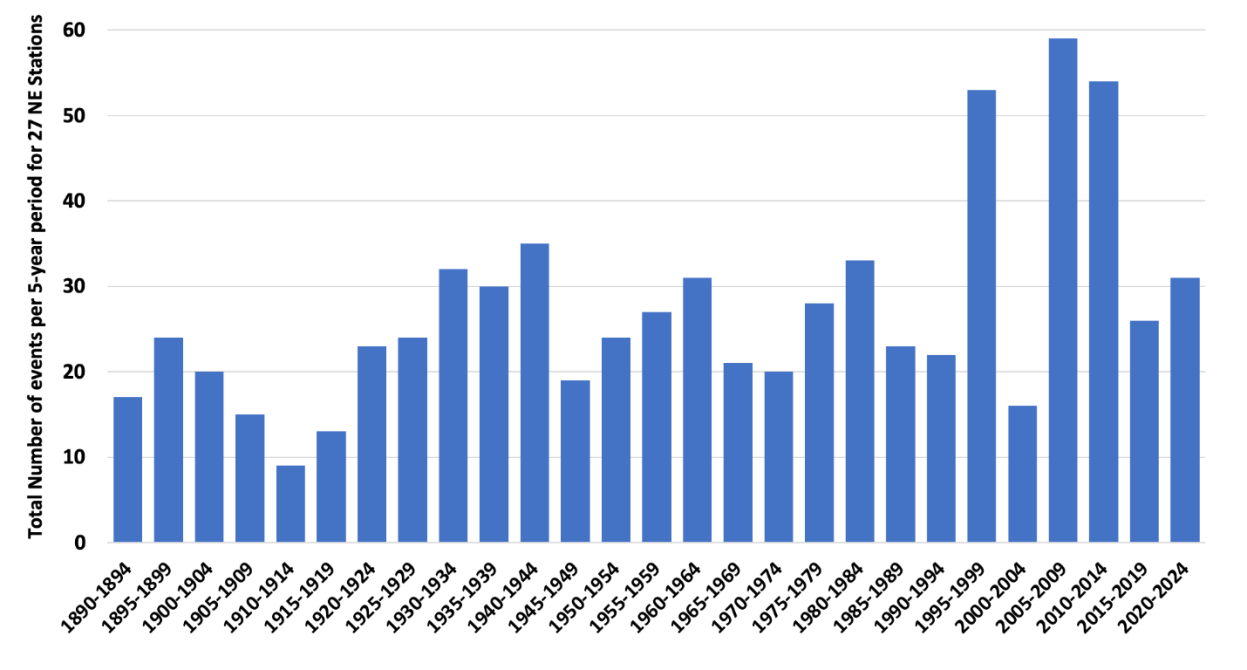
\includegraphics[width=0.9\textwidth]{bilder/bilderKlima-0058.png}\\[1cm]
\end{center}
\caption{Wie in Abb. 6.4.2, aber für die schwersten 27 (1-in-5yr) 3-Tage-Niederschlagsereignisse für 27 Nordost-Stationen von NY bis ME, einschließlich Montreal.}
\end{figure}
\begin{figure}[H]
\begin{center}
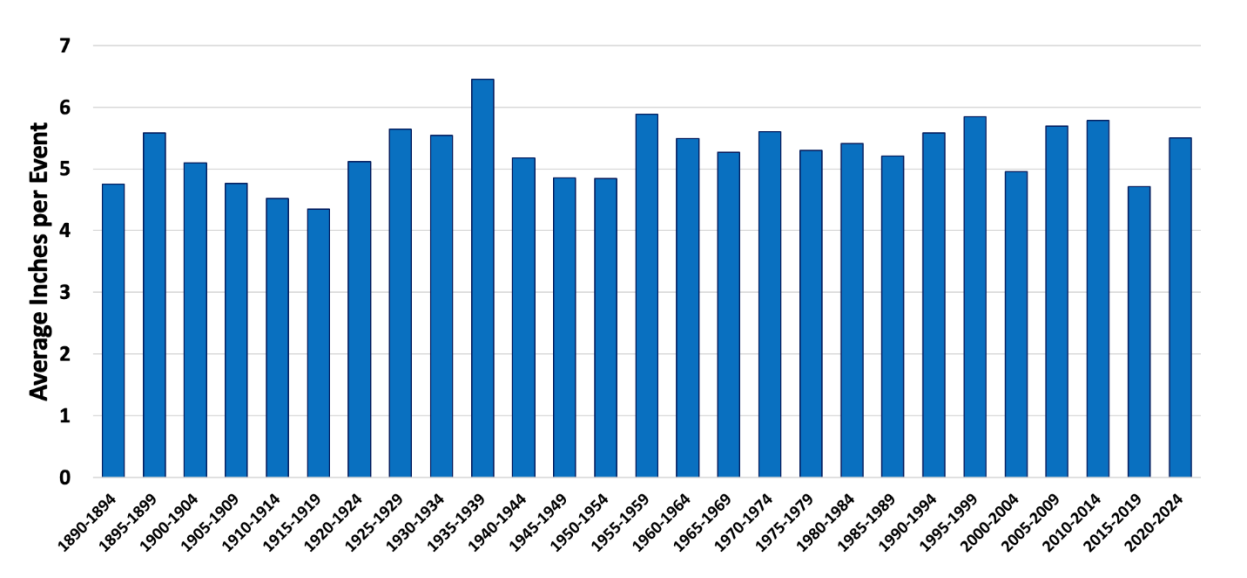
\includegraphics[width=0.9\textwidth]{bilder/bilderKlima-0059.png}\\[1cm]
\end{center}
\caption{Durchschnittliche Niederschlagsmenge, die in den 1-in-5yr-Ereignissen für die NE-Stationen fällt.}
\end{figure}

Die hohe prozentuale Zunahme in der Howarth et al. Stichprobe ist mit kleinen Zahlen an relativ wenigen Standorten verbunden: es gab nur 6 in der ersten Periode und 25 in der zweiten über 58 Stationen. Die meisten Stationen verzeichneten kein solches Ereignis. Wenn es eine regionsweite Zunahme schwerer Ereignisse gibt, sollte sie im Durchschnitt über alle Stationen gesehen werden. Abbildung 6.4.5 zeigt den durchschnittlichen Niederschlag in den 1-in-5 yr-Ereignissen über den NE. Der Trend ist nur +0,04 Zoll/Dekade. Die höchste Menge, 1935-39, schließt den Great New England Hurricane von 1938 ein, einen der seltenen schweren (Kategorie 3 oder höher) Hurrikans, die die Region trafen.

Die Ergebnisse in Abbildungen 6.4.4 und 6.4.5 deuten daher darauf hin, dass obwohl es einen Anstieg in der Anzahl von Ereignissen an wenigen Standorten während des 1995 bis 2014 Intervalls gab, gab es kein regionales Muster und die Änderung hielt nicht über 2014 hinaus an.

Jong et al. (2024) dokumentieren die Zunahme tropischer Einflüsse auf Niederschlagsereignisse im Nordosten seit 1959 und schlossen: "Der Herbst-Extremniederschlagstrend über den Nordosten der USA wird primär tropischen Wirbelsturm-verwandten Ereignissen seit den 1990er Jahren zugeschrieben." Die Frage wird dann: "War die zeitliche Häufung tropischer Systeme in 1997-2014, die den Nordosten beeinflussten, eine Antwort auf steigende THGs?" Jong et al. untersuchten CMIP-6 Modelloutput, das darauf hindeutet, dass es weniger solche Systeme im 21. Jahrhundert geben wird, aber dass die Intensität der Niederschlagsereignisse zunehmen könnte. Diese Vermutung wird nicht in Abb. 6.4.5 gesehen, wo die Menge-pro-Ereignis über die 135-jährige Periode stabil geblieben ist.

Es gibt einige Evidenz, die darauf hinweist, dass die schwersten Niederschlagsereignisse aufgrund der Auswirkung städtischer Infrastruktur auf das lokale Wetter umverteilt werden könnten (z.B., Pielke Sr. et al. 2011, Zhang et al. 2018, Yang et al. 2024). Yang et al. stellen fest: "Städte, die kompakte Entwicklung erleben, tendieren dazu, größere Zunahmen der extremen Niederschlagshäufigkeit über der Innenstadt als ihre ländlichen Umgebungen zu erleben, während die Anomalien in der extremen Niederschlagshäufigkeit für Städte mit zerstreuter Entwicklung abnehmen." Während dies eine wichtige Einsicht ist, die zu berücksichtigen ist, ist die Auswirkung auf die spezifischen Stationen, die in dieser Analyse verwendet werden, unbekannt oder zumindest nicht in Abb. 6.4.5 detektierbar.

Zusammenfassend zeigen einige US-Regionen kurzzeitige Zunahmen extremer Niederschlagsereignisse, konsistent mit natürlicher Variabilität. Aber die Analyse langfristiger, landesweiter historischer Aufzeichnungen, die die Autokorrelationseigenschaften von Niederschlagsdaten berücksichtigt, unterstützt nicht die Behauptung, dass extreme kurzzeitige Niederschlagsereignisse häufiger oder intensiver werden.

\section{Tornados}
AR6 bewertet Tornado-Trends in den USA wie folgt:

\begin{quote}
Beobachtungstrends bei Tornados, Hagel und Blitzen im Zusammenhang mit schweren konvektiven Stürmen werden nicht robust detektiert aufgrund unzureichender Abdeckung der langfristigen Beobachtungen. Es besteht mittleres Vertrauen, dass die mittlere jährliche Anzahl von Tornados in den USA relativ konstant geblieben ist." (Kapitel 11, Abschnitt 11.7.3, S. 1594)
\end{quote}

Die Überwachung schwacher Tornados hat sich über die Zeit verändert. Das Wachstum ländlicher Bevölkerungen und die zunehmende Fähigkeit, Videos mit handgehaltenen Geräten aufzunehmen, hat zu häufigeren Meldungen schwacher Tornados geführt, die minimalen Schaden verursachen. Im Gegensatz dazu wurden starke bis heftige Tornados über die Zeit konsistenter beobachtet. Beachten Sie, dass die Tornado-Stärke durch den verursachten Schaden gemessen wird, nicht durch das visuelle Erscheinungsbild des Trichters. Begrenzte Echtzeitbeobachtungsfähigkeiten in früheren Jahrzehnten verhinderten die Identifikation nicht, weil starke bis heftige Tornados viel mehr Schaden hinterlassen, der später bewertet wird, auch wenn der Tornado selbst nicht beobachtet wurde. Seit Beginn der Statistiken 1950 gab es eine erhebliche Abnahme (um etwa 50\%) der Anzahl starker bis heftiger Tornados, wie in Abb. 6.5.1a gezeigt.

Zusammenfassend gibt es einen bemerkenswerten Abwärtstrend in der Anzahl schwerer Tornados in den USA seit 1950. Nach 1990 ist die Anzahl schwacher Tornados in den USA etwa konstant geblieben; Daten davor sind unvollständig aufgrund begrenzter Überwachung.

\begin{figure}[H]
\begin{center}
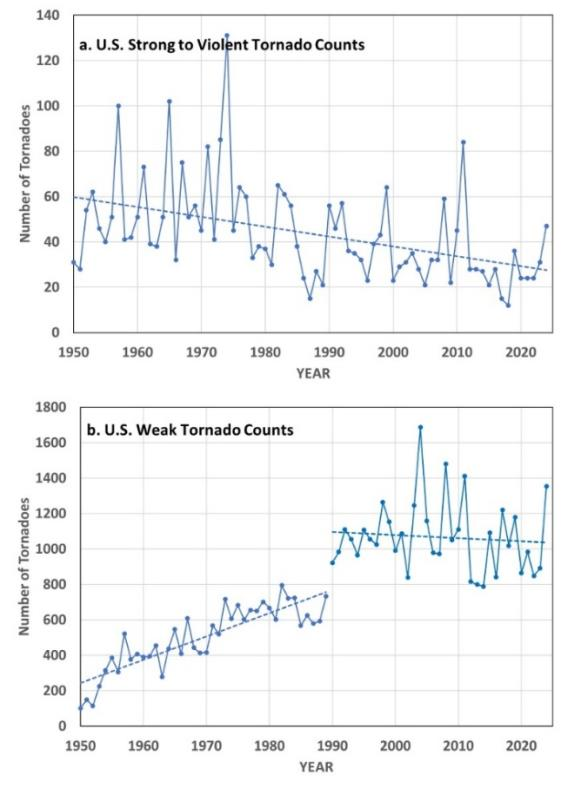
\includegraphics[width=0.9\textwidth]{bilder/bilderKlima-0060.jpg}\\[1cm]
\end{center}
\caption{Jährliche US-Tornado-Zahlen für (a) starke bis heftige Tornados (EF3 bis EF5) und (b) schwache Tornados (EF0 bis EF2). Basierend auf NOAA Storms Prediction Center Daten, verfügbar unter \url{https://www.spc.noaa.gov/wcm/data/1950-2024_actual_tornadoes.csv}}
\end{figure}

\section{Überschwemmung}
Veränderungen bei Überschwemmungen wurden wie folgt bewertet:
\begin{quote}
AR6: Der SREX \textbf{bewertete geringes Vertrauen für beobachtete Veränderungen in der Magnitude oder Häufigkeit von Überschwemmungen} auf globaler Ebene. Diese Bewertung wurde vom AR5-Bericht bestätigt. Der SR15 fand Zunahmen der Überschwemmungshäufigkeit und extremer Abflüsse in einigen Regionen, aber Abnahmen in anderen Regionen... Die hydrologische Literatur zu beobachteten Überschwemmungsveränderungen ist heterogen und konzentriert sich auf regionale und subregionale Beckenebenen, was es schwierig macht, sie auf globaler und manchmal regionaler Ebene zu synthetisieren. (Kapitel 11.5)
AR6: Die Saisonalität von Überschwemmungen hat sich in kalten Regionen verändert, wo Schneeschmelze das Abflussregime als Reaktion auf die Erwärmung dominiert (hohes Vertrauen). Das Vertrauen in Spitzenabflusstrends über vergangene Jahrzehnte auf globaler Ebene ist gering. (Kapitel 11.5)
NCA4: Trends bei extremen hohen Werten des Abflusses sind \textbf{gemischt} über die Vereinigten Staaten. Die Analyse von 200 US-Abflussmessern zeigt Gebiete sowohl zunehmender als auch abnehmender Überschwemmungsmagnitude, liefert aber \textbf{keine robusten Belege dafür}, dass diese Trends menschlichen Einflüssen zuzuschreiben sind (S. 240-241).
\end{quote}

Das Fehlen detektierbarer US-weiter Trends bei Überschwemmungen ist konsistent mit den Befunden in Abschnitt 6.4 über das Fehlen kohärenter Veränderungen bei extremen Niederschlägen.

\section{Dürren}
Bewertungen von Dürretrends waren wie folgt.

\begin{quote}
AR6: Wenige AR6-Regionen zeigen beobachtete Zunahmen meteorologischer Dürre (Abschnitt 11.9, S. 1575).

AR6: Zunehmende Trends bei landwirtschaftlichen und ökologischen Dürren wurden auf allen Kontinenten beobachtet (mittleres Vertrauen), aber Abnahmen nur in einer AR6-Region (mittleres Vertrauen). Zunehmende Trends bei hydrologischen Dürren wurden in wenigen AR6-Regionen beobachtet. (Kapitel 11 Zusammenfassung)

NCA4: Als Folge dieser erhöhten Niederschläge \textbf{sind die Dürrestatistiken über die gesamten CONUS zurückgegangen}. (S. 233)

NCA4: Jüngste Dürren und damit verbundene Hitzewellen haben in einigen Regionen der Vereinigten Staaten Rekordintensität erreicht; jedoch bleibt nach geografischem Maßstab und Dauer die Dust Bowl-Ära \textbf{der 1930er Jahre das Referenzdürre}- und extreme Hitzeereignis in der historischen Aufzeichnung (sehr hohes Vertrauen). (S. 231)

SREX: Aus einer paläoklimatischen Perspektive \textbf{sind jüngste Dürren nicht beispiellos}, mit schweren 'Megadürren', die in der paläoklimatischen Aufzeichnung für Europa, Nordamerika und Australien berichtet werden. (S. 170)
\end{quote}

\begin{figure}[H]
\begin{center}
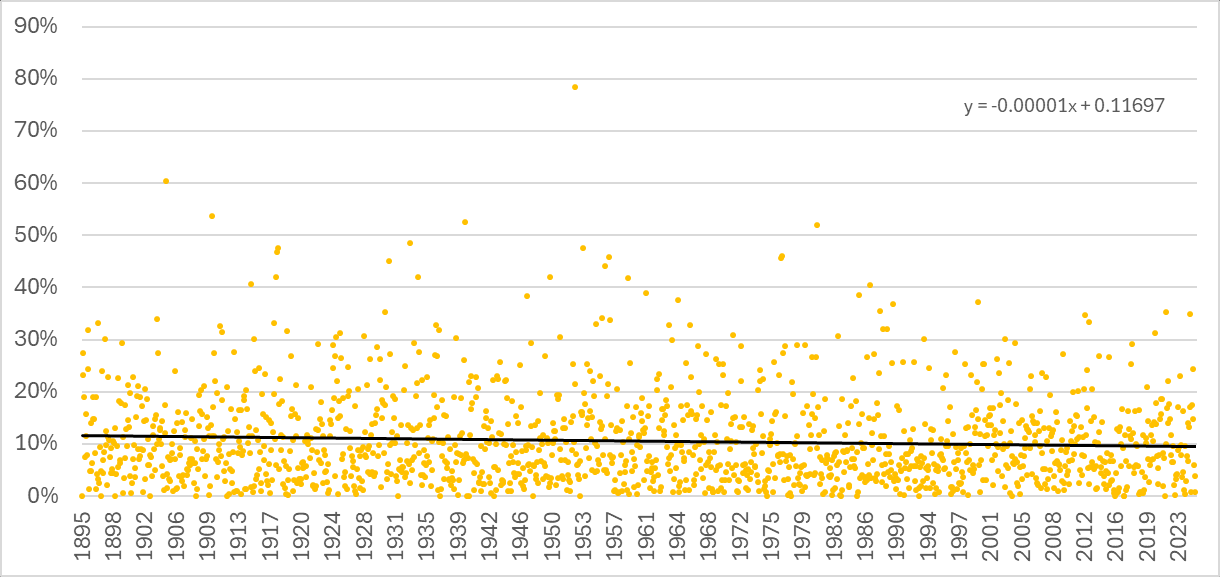
\includegraphics[width=0.9\textwidth]{bilder/bilderKlima-0061.png}\\[1cm]
\end{center}
\caption{Monatlicher Prozentsatz der USA, der als "Sehr Trocken" klassifiziert wird, 1895—2025. Datenquelle: NOAA https://www.ncei.noaa.gov/access/monitoring/uspa/wet-dry/0 Kleinste-Quadrate-Trendlinie hinzugefügt.}
\end{figure}

Wie in Abbildung 6.7.1 gezeigt, zeigen US-Langzeitdaten einen insignifikant rückläufigen Trend bei extremer Trockenheit (-0,001 Prozent pro Jahr).

Kogan et al. (2020) untersuchen ein 38-jähriges hochauflösendes satellitenbasiertes Dürremaß und schließen, dass sich die globale Dürre nicht intensiviert hat und nicht mit dem Klimawandel verbunden ist: \emph{Es ist möglich, fest zu stellen, dass die globalen und hauptgetreideländerspezifischen Dürregebiets- und Intensitätstrends nicht der globalen Klimaerwärmung seit den 1980er Jahren gefolgt sind.}

Zusammenfassend gibt es keine Evidenz für zunehmende meteorologische Dürrenhäufigkeit oder -intensität in den USA oder global über die jüngsten Jahrzehnte.

\section{Waldbrände}
Das IPCC hat keine Attributionsbewertung von Waldbränden bereitgestellt. Wie in Abbildung 6.8.1 gezeigt, zeigt die globale Waldbrand-Aktivität, gemessen von der European Space Agency, einen Abwärtstrend im 21. Jahrhundert.

\begin{figure}[H]
\begin{center}
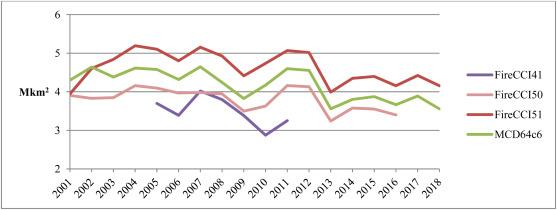
\includegraphics[width=0.9\textwidth]{bilder/bilderKlima-0063.jpg}\\[1cm]
\end{center}
\caption{Globale Waldbrandfläche 2001-2018. Quelle: Von Lizundia-Loiola et al. (2021) Abbildung 12. Die verschiedenfarbigen Linien repräsentieren Datenprodukte, die von verschiedenen Satelliten und Algorithmen abgeleitet wurden.}
\end{figure}

Globale Daten zeigen, dass die Waldbrandabdeckung auf jedem Kontinent konstant oder rückläufig ist (Samborska und Ritchie, 2024). Jedoch gibt es Evidenz, dass die Intensität von Bränden in einigen Regionen sich verschlechtert (Cunningham et al. 2024) und dass Waldbrände zu einem Nettoverlust der globalen Waldbedeckung über 2001-2019 führten (Tyukavina et al. 2022).

Aktive Feuerunterdrückung seit 1900 macht es schwierig, eine natürliche Grundlinie für Waldbrand-Aktivität in den USA zu etablieren. Paläoklimatische Evidenz zeigt, dass vergangene Aktivität viel höher war als heute. Marlon et al. (2012) verwendeten sedimentäre Kohleschichten, um die Feuergeschichte der westlichen USA für die letzten 1400 Jahre zu rekonstruieren und passten auch ein Modell an, um Feueraktivität als Funktion klimatischer Bedingungen vorherzusagen. Ihre Ergebnisse sind in Abbildung 6.8.2 unten zusammengefasst (von Abbildung 2 in ihrer Arbeit). Es gab ein wachsendes Waldbranddefizit über das 20. Jahrhundert. Mit anderen Worten, wie viel Feuer auch immer im 20. Jahrhundert beobachtet wurde, es war weniger als das, was in früheren Jahrhunderten basierend auf den klimatischen Bedingungen beobachtet worden wäre. Parks et al. (2025) finden ebenso, dass trotz der jüngsten Zunahme der Waldbrand-Brandfläche in Nordamerika ein erhebliches Waldbranddefizit relativ zu historischen Waldbrandregimen bestehen bleibt.

\begin{figure}[H]
\begin{center}
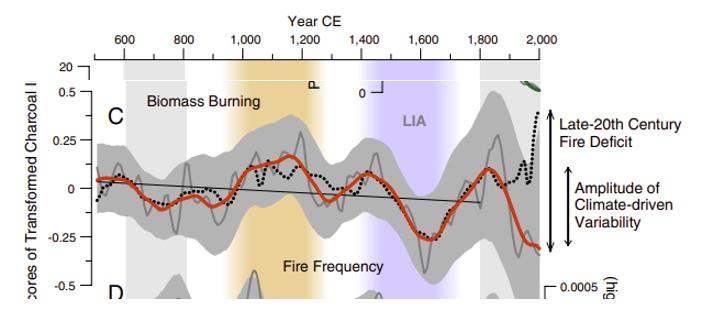
\includegraphics[width=0.9\textwidth]{bilder/bilderKlima-0064.jpg}\\[1cm]
\end{center}
\caption{Feuerhäufigkeit und Feuerdefizit in den USA. Die rote Linie zeigt die geglättete Kohleaufzeichnung und die schwarze gepunktete Linie zeigt die vorhergesagte Kohleaufzeichnung basierend auf klimatischen Bedingungen. Modell. Quelle: Marlon et al. (2012) Abbildung 2.}
\end{figure}

US-Daten des National Interagency Fire Centre (NIFC) von 1926 bis 2023 sind in Abbildung 6.8.3 gezeigt. Das NIFC hat die Daten vor 1960 von seiner aktuellen Website entfernt mit der Begründung, dass sich die Messmethoden nach 1960 änderten, wodurch der Vergleich unzuverlässig wird. Dennoch, nur auf das Intervall nach 1985 fokussierend, nimmt die Anzahl der Brände nicht zu. Die verbrannte Fläche nahm zu, aber nur bis etwa 2007.

Waldbrände waren schon immer ein Teil der Natur, und sie können sicherlich Bedingungen schaffen, die kurzfristig für alles Leben, einschließlich Menschen, unwirtlich sind. Die Wissenschaft hat den allgemeinen Nutzen und die Notwendigkeit von Waldbränden bestätigt. Während jüngste hochkarätige Brände und Saisons als Erinnerung an die potenzielle zerstörerische Auswirkung dienen, bleibt der hochkarätigste US-Waldbrand das 1910 Big Blowup-Feuer im US-Westen, das über drei Millionen Acres zerstörte und ganze Städte wie Taft, MT eliminierte (Apple, 2020). Das 1910-Feuer formte den US Forest Service um (National Forest Foundation 2022), was zu einem Fokus auf Feuerunterdrückung mit dem primären Ziel führte, alle Waldbrände zu besiegen (Forest History Society, 2022). Dies führte zur "10-Uhr-Regel" in 1935, die erforderte, dass alle an einem Tag entdeckten Brände bis 10 Uhr am folgenden Tag kontrolliert werden mussten (National Forest Foundation, 2022).

Während die Bekämpfung aller Brände ein edles Ziel schien, begannen Fragen darüber aufzukommen, ob dieses Verhalten "der Wissenschaft folgte" (U.S. Forest Service, 2022). Über die Zeit hat der US Forest Service begonnen, seine Ziele zu überdenken und zu erkennen, dass neue Ansätze wie verschriebene Brände, Brennstoffelimination und kontrollierte Waldbrände angemessener sind (Sommer, 2016). Jüngste Forschung validiert diesen Ansatz und erkennt, dass häufigere kleinere Brände wahrscheinlich zu gesünderen Wäldern, Wasserökosystemen und Biodiversität führen (Stephens et al., 2021).

\begin{figure}[H]
\begin{center}
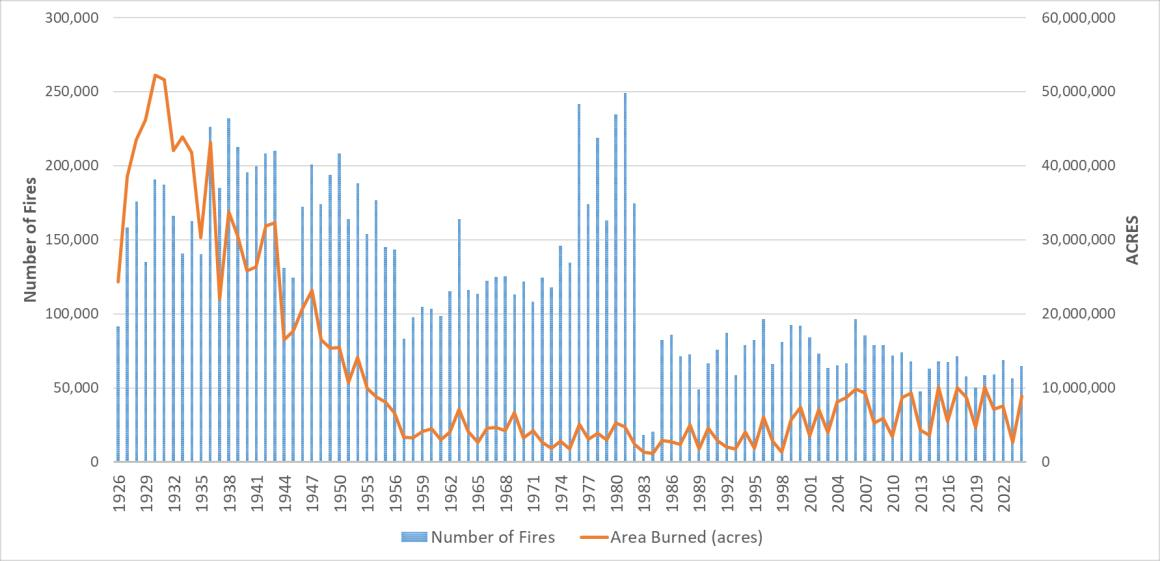
\includegraphics[width=0.9\textwidth]{bilder/bilderKlima-0065.jpg}\\[1cm]
\end{center}
\caption{US-Waldbrände 1926 bis 2023. Quelle: Nach 2018: National InterAgency Fire Center Daten https://www.nifc.gov/fire-information/statistics/wildfires. Vor 2017 webarchive.org (n.d.).}
\end{figure}

\vfill
\noindent\textbf{Literaturverzeichnis:}

\begingroup
\parindent=0pt
\everypar{\hangindent=2em\hangafter=1\relax}

Apple, C. (2020, January 21). 1910 fire – The big burn across Montana and Idaho. The Spokesman-
Review. https://www.spokesman.com/stories/2020/jan/19/1910-fire-big-burn-across-montana-and-
idaho/

Bell, Gerald D. and Muthuvel Chelliah, “Leading Tropical Modes Associated with Interannual and
Multidecadal Fluctuations in North Atlantic Hurricane Activity,” Journal of Climate 19, no. 4
(February 15, 2006): 590–612, https://doi.org/10.1175/JCLI3659.1.

Brewer, W. H. (1930). Up and down California in 1860–1864: The journal of William H. Brewer.
University of California Press.

Christy, J. R., Norris, W. B., and McNider, R. T. (2009). Surface temperature variations in East Africa
and possible causes. Journal of Climate, 22(12), 3342–3356. https://doi.org/10.1175/2008JCLI2726.1

Cohn, T. A. and Lins, H. F. (2005). Nature’s style: Naturally trendy. Geophysical Research Letters,
32(23). https://doi.org/10.1029/2005GL024476

Colorado State University. (2025). Realtime tropical cyclone guidance.
\url{https://tropical.atmos.colostate.edu/Realtime/index.php}

Cunningham, C.X., G.J. Williamson, and D. Bowman (2024) Increasing frequency and intensity of the
most extreme wildfires on Earth. Nature Ecology and Evolution 8, 1420–1425.
https://doi.org/10.1038/s41559-024-02452-2

Forest History Society (2022). The 1910 fires. https://foresthistory.org/research-explore/us-forest-service-
history/policy-and-law/fire-u-s-forest-service/famous-fires/the-1910-fires/

Gershunov, A., and K. Guirguis (2012). California heat waves in the present and future. Geophysical
Research Letters, 39(18). https://doi.org/10.1029/2012GL052979

Gershunov, A., T. Shulgina, F.M. Ralph, D.A. Lavers J.J. and Rutz (2017). Assessing the climate-scale
variability of atmospheric rivers affecting western North America. Geophysical Research Letters,
44(15), 7900–7908. https://doi.org/10.1002/2017GL074175

Goldenberg, Stanley et al., “The Recent Increase in Atlantic Hurricane Activity: Causes and
Implications,” Science 293, no. 5529 (July 20, 2001): 474–479,
\url{https://doi.org/10.1126/science.1060040.}

Howarth, M. E., C.D. Thorncroft, and L.F. Bosart (2019). Changes in extreme precipitation in the
Northeast United States: 1979–2014. Journal of Hydrometeorology, 20(4), 673–689.
https://doi.org/10.1175/JHM-D-18-0155.1

Hurst, H. E. (1951). Long term storage capacities of reservoirs. Transactions of the American Society of
Civil Engineers, 116, 776–808.

Intergovernmental Panel on Climate Change (IPCC). (2021). Climate change 2021: The physical science
basis. Contribution of Working Group I to the Sixth Assessment Report of the Intergovernmental
Panel on Climate Change (V. Masson-Delmotte et al., Eds.). Cambridge University Press.
https://www.ipcc.ch/report/ar6/wg1/

Jong, B.-T., H. Murakami, T.L. Delworth and W.F. Cooke (2024). Contributions of tropical cyclones and
atmospheric rivers to extreme precipitation trends over the Northeast US. Earth’s Future, 12,
e2023EF004370. https://doi.org/10.1029/2023EF004370

Karl, T.R., H.F. Diaz, and G. Kukla. (1988): Urbanization: Its detection and effect on the United States
climate record. Journal of Climate, 1, 1099-1123
\url{https://journals.ametsoc.org/view/journals/clim/1/11/1520-
0442_1988_001_1099_uidaei_2_0_co_2.xml}

Karl, T. R., C.N. Williams Jr., F.T. Quinlan, and T.A. Boden (1990). United States Historical
Climatology Network (HCN) serial temperature and precipitation data (Publication No. 3404). Oak
Ridge National Laboratory.

Klotzbach, Phil et al. (2018) Continental U.S. Hurricane Landfall Frequency and Associated Damage:
Observations and Future Risks, Bulletin of the American Meteorological Society 99, no. 7 (July
2018): 1359–1376, https://doi.org/10.1175/BAMS-D-17-0184.1.

Kogan, Feliz, Wei Guob and Wenze Yang (2020) “Near 40-year drought trend during 1981-2019 earth
warming and food security” Geomatics, Natural Hazards and Risk Vol 11(1)

Koutsoyiannis, D. (2013) Hydrology and Change. Hydrological Sciences Journal 58(6)
http://dx.doi.org/10.1080/02626667.2013.804626

Lizundia-Loiola, J., et al. (2020) A spatio-temporal active-fire clustering approach for global burned area
mapping at 250 m from MODIS data. Remote Sensing of the Environment 236, 111493,
https://doi.org/10.1016/j.rse.2019.111493

Markonis, Y., and D. Koutsoyiannis (2016). Scale-dependence of persistence in precipitation records.
Nature Climate Change, 6, 399–401. https://doi.org/10.1038/nclimate2894

Marlon, Jennifer, Patrick J Bartlein, Daniel G. Gavin et al. (2012) Long-term perspective on wildfires in
the western USA Proceedings of the National Academy of Sciences February 14 2012
https://www.pnas.org/doi/pdf/10.1073/pnas.1112839109

Maue, R. N. (2025). Climatlas: Tropical cyclones. https://climatlas.com/tropical/

Maue, R. N. (2011) Recent historically low tropical cyclone activity. Geophysical Research Letters 38,
L14803, doi:10.1029/2011GL047711

McKitrick, R., and J.R. Christy (2019). Assessing changes in US regional precipitation on multiple time
scales. Journal of Hydrology, 578, 124074. \url{https://doi.org/10.1016/j.jhydrol.2019.124074}

McKitrick, R. and J.R. Christy (2025), “Data and Code for CWG2025 Report”, Mendeley Data, V1, doi:
10.17632/by76s7rxfb.1

McNider, R.T., G.J. Steeneveld, A.A.M. Holtslag, R.A. Pielke Sr., S. Mackaro, A. Pour-Biazar, J.
Walters, U. Nair, and J.R. Christy, 2012: Response and sensitivity of the nocturnal boundary layer
over land to added longwave radiative forcing. Journal of Geophysical Research., 117, D14106,
doi:10.1029/2012JD017578.

Null, J. and J. Hulbert, “California Washed Away: The Great Flood of 1862,” Weatherwise 60, no. 1
(2007): 26–30, https://doi.org/10.3200/wewi.60.1.26-30

National Forest Foundation. (2022). Blazing battles: The 1910 fire and its legacy.
\url{https://www.nationalforests.org/our-forests/your-national-forests-magazine/blazing-battles-the-1910-
fire-and-its-legacy}

National Interagency Fire Center. (2024). Wildfire statistics. https://www.nifc.gov/fire-
information/statistics/wildfires

NCA4. (2017). Climate science special report: Fourth National Climate Assessment, Volume I (D. J.
Wuebbles, D. W. Fahey, and K. A. Hibbard, Eds.). U.S. Global Change Research Program.
https://doi.org/10.7930/J0J964J6

NCA5. (2023). Fifth National Climate Assessment (A. R. Crimmins et al., Eds.). U.S. Global Change
Research Program. https://doi.org/10.7930/NCA5.2023.CH1 (accessed May 22, 2025)

NOAA Hurricane Research Division. (2025a). All U.S. hurricanes (1851–2019).
\url{https://www.aoml.noaa.gov/hrd/hurdat/All_U.S._Hurricanes.html}

NOAA Hurricane Research Division. (2025b). Most intense (3, 4, 5) continental United States
hurricanes: 1851–1970, and 1983–2023. \url{https://www.aoml.noaa.gov/hrd/hurdat/most_intense.html}

Overland, J. E. (2021). Causes of the record-breaking Pacific Northwest heatwave, late June 2021.
Atmosphere, 12(11), 1434. https://doi.org/10.3390/atmos12111434

Pan, M., M. Lu and U. Lall (2024). Diversity of cross-Pacific atmospheric river main routes.
Communications Earth and Environment, 5, 378. https://www.nature.com/articles/s43247-024-
01552-y

Parks, Sean, Christopher Guiterman, Ellis Margolis et al. (2025) A fire deficit persists across diverse
North American forests despite recent increases in area burned. Nature Communications 16
\url{https://www.nature.com/articles/s41467-025-56333-8}

Pielke, R. A., et al. (2011). Land use/land cover changes and climate: Modeling analysis and
observational evidence. Wiley Interdisciplinary Reviews: Climate Change, 2, 828–850.
https://doi.org/10.1002/wcc.144

Porter, K., et al. (2011). Overview of the ARkStorm scenario. U.S. Geological Survey.

Quinlan, F. T., T. R. Karl, and C.N. Williams Jr. (1987). United States Historical Climatology Network
(USHCN) serial temperature and precipitation data (NDP-019). Oak Ridge National Laboratory.

Runnalls, K.E. and T.R. Oke, 2006: Technique to detect microclimate inhomogeneities in historical
records of screen-level air temperature. Journal of Climate, 19, 959-978.
\url{https://doi.org/10.1175/JCLI3663.1}

Samborska, V., and H. Ritchie (2024). Wildfires. Our World in Data. \url{https://ourworldindata.org/wildfires}

Seneviratne, S. et al. (2021) “Chapter 11: Weather and Climate Extreme Events in a Changing Climate.”
In Climate Change 2021: The Physical Science Basis. Contribution of Working Group I to the Sixth
Assessment Report of the Intergovernmental Panel on Climate Change, edited by V. Masson-
Delmotte, P. Zhai, A. Pirani, S.L. Connors, C. Péan, S. Berger, N. Caud, et al., 1513–1766.
Cambridge: Cambridge University Press, 2021. https://doi.org/10.1017/9781009157896.013.

Sommer, L. (2016, November 7). Let it burn: The Forest Service wants to stop putting out some fires.
KQED. https://www.kqed.org/science/1134217/let-it-burn-the-forest-service-wants-to-stop-putting-
out-some-fires

Stephens, Scott et al., (2021) “Fire, Water, and Biodiversity in the Sierra Nevada: A Possible Triple Win,”
Environmental Research Communications 3, no. 8 (August 6, 2021): p. 081004,
https://doi.org/10.1088/2515-7620/ac17e2.

Tyukavina Alexandra , Peter Potapov, Matthew Hansen et al. (2022) Global Trends of Forest Loss Due to
Fire From 2001 to 2019, Frontiers in Remote Sensing. Volume 3
\url{https://www.frontiersin.org/journals/remote-sensing/articles/10.3389/frsen.2022.825190/full}

U.S. Forest Service. (2022). Managing fire. https://www.fs.usda.gov/science-technology/fire

USGCRP. (2023). USGCRP indicators platform: Heat waves.
\url{https://www.globalchange.gov/indicators/heat-waves}

Vecchi, Gabriel A. and Thomas R. Knutson (2011) “Estimating Annual Numbers of Atlantic Hurricanes
Missing from the HURDAT Database (1878–1965) Using Ship Track Density,” Journal of Climate
24, no. 6 (2011): 1736–1746, https://doi.org/10.1175/2010JCLI3810.1.

Villarini, Gabriele, Gabriel A. Vecchi, and James A. Smith, “U.S. Landfalling and North Atlantic
Hurricanes: Statistical Modeling of Their Frequencies and Ratios,” Monthly Weather Review 140, no.
1 (January 2012): 44–65, https://doi.org/10.1175/MWR-D-11-00063.1.

Web Archive. (n.d.). Archive of NIFC fire data.
\url{https://web.archive.org/web/20200212033452/https://www.nifc.gov/fireInfo/fireInfo_stats_totalFires.
html}

Yang, L., Y. Yang, Y. Shen, et al. (2024). Urban development pattern’s influence on extreme rainfall
occurrences. Nature Communications, 15, 3997. https://doi.org/10.1038/s41467-024-48533-5

Zhang, W., G. Villarini, G.A. Vecchi, and J.A. Smith, J. A. (2018). Urbanization exacerbated the rainfall
and flooding caused by Hurricane Harvey in Houston. Nature, 563, 384–388.
https://doi.org/10.1038/s41586-018-0676-z
\endgroup


\cleardoublepage
\FigureNumbersByChapter 
\chapter{VERÄNDERUNGEN DES MEERESSPIEGELS}
\paragraph{Kapitelzusammenfassung}
\begin{quote}
Seit 1900 ist der globale durchschnittliche Meeresspiegel um etwa 8 Zoll gestiegen. Meeresspiegeländerungen entlang der US-Küsten sind sehr variabel und stehen in Verbindung mit lokalen Variationen in Prozessen, die zum Absinken beitragen, sowie mit Meeresströmungsmustern. Die größten Meeresspiegelanstiege entlang der US-Küsten sind in den Regionen Galveston, New Orleans und der Chesapeake Bay - jeder dieser Orte ist mit erheblichem lokalem Landabsinken (Subsidenz) verbunden, das nicht mit dem Klimawandel zusammenhängt.

Extreme Projektionen des globalen Meeresspiegelanstiegs sind mit einem unplausiblen extremen Emissionsszenario und der Einbeziehung schlecht verstandener Prozesse verbunden, die mit hypothetischen Eisschild-Instabilitäten zusammenhängen. Bei der Bewertung der AR6-Projektionen bis 2050 (mit Bezug auf die Referenzperiode 1995-2014) ist bis 2025 fast die Hälfte des Intervalls verstrichen, wobei der Meeresspiegel langsamer ansteigt als vorhergesagt. US-Pegelmessungen zeigen keine offensichtliche Beschleunigung über die historische durchschnittliche Rate des Meeresspiegelanstiegs hinaus.
\end{quote}

\section{Globaler Meeresspiegelanstieg}
Der globale Meeresspiegelanstieg ist wohl der wichtigste klimatische Wirkungsfaktor, der eindeutig mit steigenden Temperaturen verbunden ist. Auf globaler Ebene erhöht die Erwärmung den Meeresspiegel durch thermische Expansion des Meerwassers und durch das Schmelzen von Gletschern und Eisschilden. Variationen in der Landwasserspeicherung sind ein weiterer wichtiger Faktor. Auf regionaler Ebene wird die Meeresspiegeländerung von großräumigen Meeresströmungsmustern und geologischen Prozessen und Verformungen durch die Umverteilung von Eis und Wasser beeinflusst. Lokal sind auch vertikale Landbewegungen durch geologische Prozesse, Grundwasserentnahme und Förderung fossiler Brennstoffe wichtig.

AR6 schätzt, dass der globale mittlere Meeresspiegel zwischen 1901 und 2018 um 7,9 (5,9–9,8) Zoll gestiegen ist, wobei sich die Rate des Meeresspiegelanstiegs in den letzten Jahrzehnten beschleunigt hat. Auf der Ebene der Ozeanbecken sind die Meeresspiegel im Zeitraum 1993–2018 am schnellsten im Westpazifik und am langsamsten im Ostpazifik gestiegen (Fox-Kemper et al., 2021). Die Rate des globalen Meeresspiegelanstiegs wird auf 0,12 Zoll/Jahr geschätzt, etwa die Höhe von zwei übereinander gestapelten Pfennigen (NASA, 2020).

Die Beobachtungssysteme für den globalen Meeresspiegelanstieg haben sich im Satellitenzeitalter erheblich verbessert, insbesondere mit dem Aufkommen von Satellitenaltimetern im Jahr 1993. Lokale Pegel haben für das vergangene Jahrhundert nützliche Daten geliefert, und für einige wenige Orte sogar noch länger. Nach dem Ende der Kleinen Eiszeit Mitte des neunzehnten Jahrhunderts zeigen Pegel, dass der globale mittlere Meeresspiegel während der Periode 1820–1860 zu steigen begann, deutlich vor den meisten anthropogenen Treibhausgasemissionen.

\section{US-Meeresspiegelanstieg}
Beobachtete und vorhergesagte Raten des mittleren globalen Meeresspiegelanstiegs könnten aufgrund lokaler Prozesse für spezifische Standorte wenig wissenschaftliche Relevanz haben (NOAA, 2025). Abbildung 7.1 zeigt, dass in Kanada und Alaska (und auch im nördlichen Washington) der Meeresspiegel sinkt, aufgrund von Anhebung durch glaziale Erholung. Die meisten Pegel an der Pazifikküste zeigen niedrige Raten des Meeresspiegelanstiegs, während die größten US-Raten an der Golfküste (Louisiana und Texas) und in den mittelatlantischen Staaten (Chesapeake Bay-Region) auftreten.

\begin{figure}[H]
\begin{center}
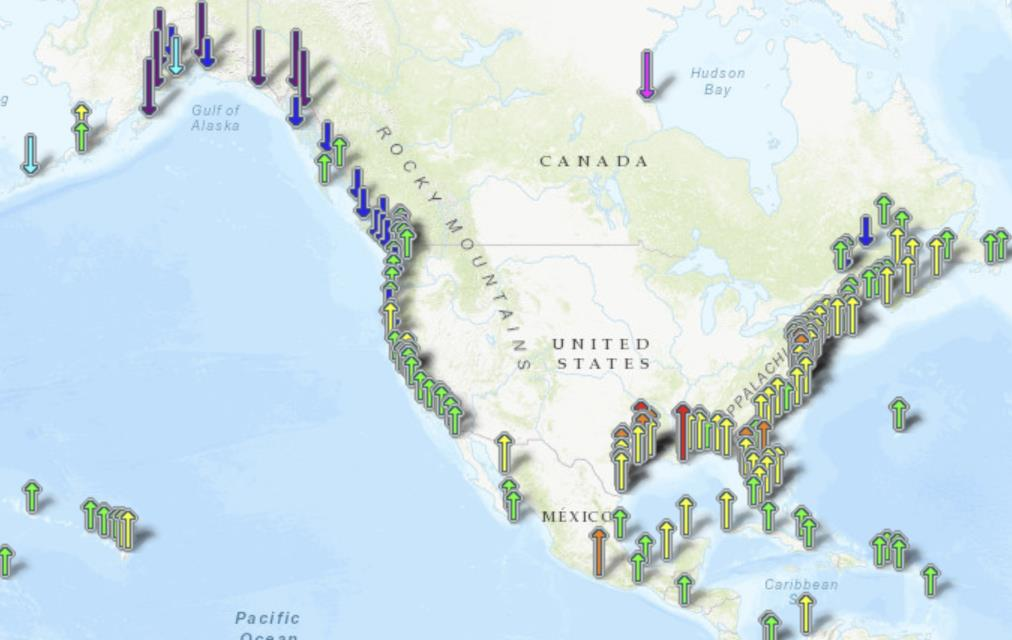
\includegraphics[width=0.9\textwidth]{bilder/bilderKlima-0067.jpg}\\[1cm]
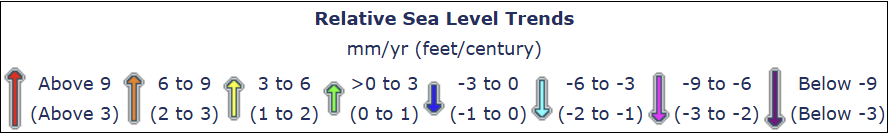
\includegraphics[width=0.9\textwidth]{bilder/bilderKlima-0068.png}\\[1cm]
\end{center}
\caption{Karte der Raten des relativen Meeresspiegelanstiegs entlang der US-Küste (NOAA, https://tidesandcurrents.noaa.gov/sltrends/). Zum Vergleich: 3 mm = 0,12 Zoll.}
\end{figure}

Messungen des relativen Meeresspiegelanstiegs durch Pegel vermischen die klimatologisch relevante Zunahme des Meerwasservolumens mit lokalen vertikalen Landbewegungen. Letztere, die von Ort zu Ort variieren, werden am besten mit einer Global Positioning System (GPS)-Station gemessen, die sich nahe dem Pegel befindet. Sie werden von einer Reihe von Prozessen angetrieben, die mit dem Klimasignal vergleichbar sein können und lokal das Risiko des Meeresspiegelanstiegs verschärfen (Subsidenz/Absinken) oder mildern (Anhebung) können (Wöppelmann und Marcos, 2016). Menschliche Aktivitäten, die Subsidenz auslösen, sind oft bedeutsam. Dazu gehören Bodenentwässerung (z.B. für städtische Entwicklung) und unterirdische Entnahme von Grundwasser oder Kohlenwasserstoffen.

Tabelle 7.1 zeigt den absoluten Meeresspiegelanstieg (ASLR) für ausgewählte Standorte, bestimmt aus der Summe des unkorrigierten relativen Meeresspiegelanstiegs (RSLR), wie er aus Pegelzeitreihen geschätzt wurde (NOAA, 2025), und den Messungen der vertikalen Landbewegung (VLM) (NAS, 2012; Letetrel et al., 2015; Karegar et al., 2016). Der absolute Meeresspiegelanstieg für jeden dieser Standorte ist aufgrund lokaler Subsidenz erheblich kleiner als der gemessene relative Meeresspiegelanstieg. Mehr als die Hälfte des gemessenen relativen Meeresspiegelanstiegs wird dem Landabsinken zugeschrieben für diese Standorte: San Francisco, Galveston, Grand Isle. Zum Vergleich wird die globale durchschnittliche Rate des absoluten Meeresspiegelanstiegs auf 0,12 Zoll/Jahr geschätzt.

%%Tabelle
\vspace{3ex}
\noindent
\begin{minipage}{\textwidth}
  \sisetup{retain-explicit-plus = true}
  \centering
  \begin{tabular}{
        l
        S[table-format=+1.2]
        S[table-format=+1.2]
        S[table-format=+1.2]
  }
    \toprule
    \multicolumn{1}{l}{Standort} &
    \multicolumn{1}{c}{RSLR} &
    \multicolumn{1}{c}{VLM} &
    \multicolumn{1}{c}{ASLR} \\
    \midrule
    San Francisco     &  +0.08 & -0.06 & +0.02 \\
    Galveston, TX     &  +0.26 & -0.19 & +0.07 \\
    Grand Isle, LA    &  +0.36 & -0.28 & +0.08 \\
    Petersburg, FL    &  +0.12 & -0.02 & +0.10 \\
    New York City, NY &  +0.11 & -0.05 & +0.06 \\
    \bottomrule
  \end{tabular}
  \captionof{table}{Absoluter Meeresspiegelanstieg (Zoll/Jahr) bestehend aus relativem Meeresspiegelanstieg (RSLR) plus vertikaler Landbewegung (VLM)}
  \label{tab:chap7}
\end{minipage}


\subsection*{San Francisco Bay}
In den vergangenen 100 Jahren ist der relative Meeresspiegel in der San Francisco Bay-Region um 7,8 Zoll gestiegen, mit einer durchschnittlichen Rate von 0,08 Zoll/Jahr (Abbildung 7.2). Wie in Tabelle 7.1 gezeigt, beträgt San Franciscos vertikale Landbewegung -0,06 Zoll/Jahr (Absinken), was eine jüngste absolute Rate von +0,02 Zoll/Jahr ergibt. Teile von Treasure Island, San Francisco International Airport und Foster City sinken um bis zu 0,4 Zoll/Jahr (Shirzaei und Bürgmann, 2018). Probleme in der San Francisco Bay-Region, einschließlich Bedrohungen für den Flughafen, werden hauptsächlich durch Bodenverdichtung in Aufschüttungszonen verursacht, die früher Feuchtgebiete waren, nicht durch das langsame Kriechen des globalen Meeresspiegelanstiegs.

\begin{figure}[H]
\begin{center}
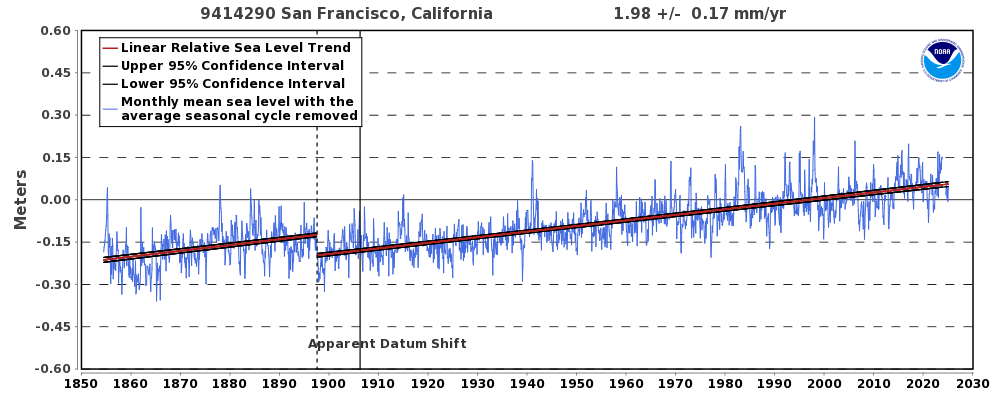
\includegraphics[width=0.9\textwidth]{bilder/bilderKlima-0069.png}\\[1cm]
\end{center}
\caption{Pegelmessungen in San Francisco, Kalifornien, erhalten von NOAA - \url{https://tidesandcurrents.noaa.gov/sltrends/sltrends_station.shtml?id=9414290} (heruntergeladen 4/22/25).}
\end{figure}

\subsection*{Galveston - Houston}
Langzeitmessungen des Pegels am Galveston Pier 21 zeigen einen Meeresspiegelanstieg von 2,18 Fuß im vergangenen Jahrhundert oder eine Rate von 0,26 Zoll/Jahr (Abbildung 7.3). Die vertikale Landbewegung (Subsidenz) in Galveston wird auf -0,19 Zoll/Jahr geschätzt, was eine absolute Anstiegsrate von +0,07 Zoll/Jahr ergibt (Tabelle 7.1). Der U.S. Geological Survey fand heraus, dass der größte Teil der Oberflächensubsidenz in der Houston-Galveston-Region ein direktes Ergebnis von Grundwasserentnahmen ist (Kasmarek und Ramage 2017), die eine Verdichtung der Aquifer-Sedimente verursachten, hauptsächlich in den feinkörnigen Schluff- und Tonschichten. Bis 1979 war in Houston eine Subsidenz von bis zu 10 Fuß aufgetreten.

\begin{figure}[H]
\begin{center}
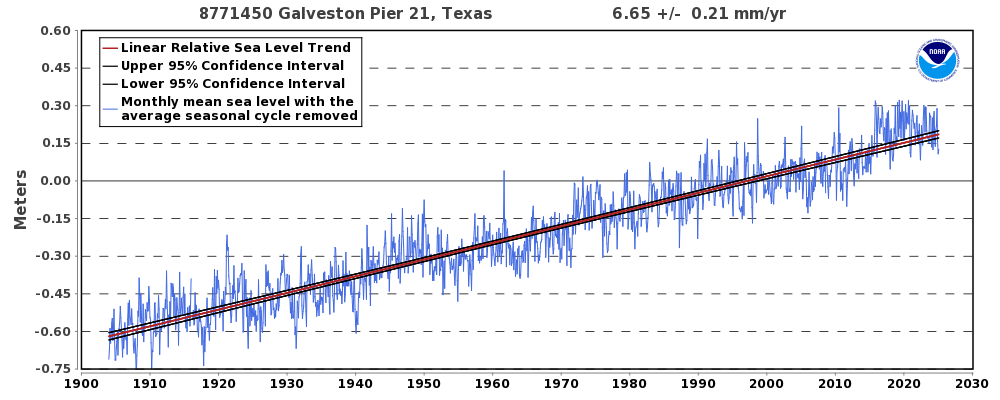
\includegraphics[width=0.9\textwidth]{bilder/bilderKlima-0070.png}\\[1cm]
\end{center}
\caption{Pegelmessungen Galveston Pier, TX, erhalten von NOAA - \url{https://tidesandcurrents.noaa.gov/sltrends/sltrends_station.shtml?id=8771450} (heruntergeladen 4/22/2025).}
\end{figure}

\subsection*{New Orleans und das Mississippi-Delta}
Langzeitmessungen des Pegels in Grand Isle, Louisiana, zeigen, dass der Meeresspiegel in den letzten 100 Jahren um etwas mehr als 3 Fuß gestiegen ist, mit einer durchschnittlichen Rate von 0,36 Zoll/Jahr (Abbildung 7.4).
Die vertikale Landbewegung (Subsidenz) wird auf -0,28 Zoll/Jahr geschätzt. Tabelle 7.1 gibt den absoluten Meeresspiegelanstieg mit +0,08 Zoll/Jahr an.

\begin{figure}[H]
\begin{center}
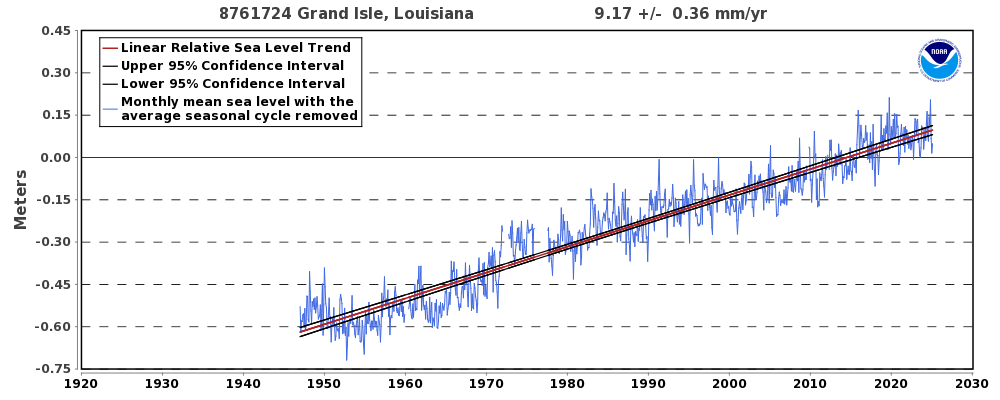
\includegraphics[width=0.9\textwidth]{bilder/bilderKlima-0071.png}\\[1cm]
\end{center}
\caption{Pegelmessungen in Grand Isle, LA, erhalten von NOAA - \url{https://tidesandcurrents.noaa.gov/sltrends/sltrends_station.shtml?id=8761724} (heruntergeladen 4/22/25).}
\end{figure}

Die Probleme des Meeresspiegelanstiegs und Landverlusts in der Mississippi-Delta-Region sind komplex, wobei geologische Subsidenz und der Rückgang der vom Mississippi River transportierten Sedimente die dominierenden Treiber sind. Der Bau von Dämmen im Einzugsgebiet seit den 1950er Jahren hat die Schwebstoff-Fracht des Mississippi um ~50 Prozent verringert (Maloney 2018). Eine neue Subsidenzkarte des Küstengebiets von Louisiana zeigt, dass die Küstenregion um etwa ein Drittel Zoll pro Jahr absinkt (Neinhuis et al. 2017), verbunden mit Grundwasser- und Ressourcenentnahme. Da die Höhenlage der Stadt im Durchschnitt ein bis zwei Fuß unter dem Meeresspiegel liegt, ist der Meeresspiegelanstieg durch anthropogene Erwärmung kaum der dominierende Treiber von New Orleans' Problemen.

\subsection*{New York City}
New York City ist besonders verwundbar gegenüber den Auswirkungen des Meeresspiegelanstiegs, weil es hauptsächlich auf Inseln gebaut ist und 520 Meilen Küstenlinie hat. Messungen durch einen Pegel an der Südspitze von Manhattan (The Battery) zeigen, dass der relative Meeresspiegel in den vergangenen Jahrhundert um über 11 Zoll gestiegen ist, mit einer durchschnittlichen Rate von 0,11 Zoll/Jahr (Abbildung 7.5). Aber die vertikale Landbewegung in der New York City-Region beträgt -0,05 Zoll/Jahr (ungefähr 5 Zoll pro Jahrhundert), so dass die absolute Rate des Meeresspiegelanstiegs am Battery 0,06 Zoll/Jahr beträgt, oder etwa 55 Prozent des gemessenen relativen Meeresspiegelanstiegs.

\begin{figure}[H]
\begin{center}
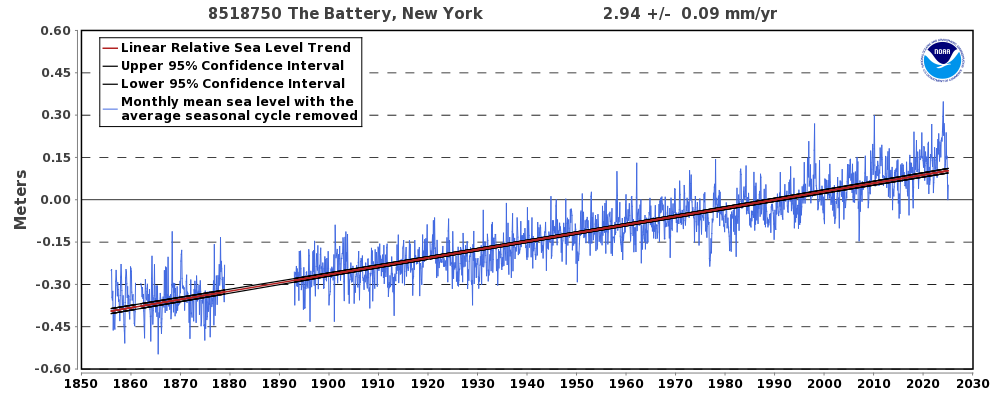
\includegraphics[width=0.9\textwidth]{bilder/bilderKlima-0072.png}\\[1cm]
\end{center}
\caption{Pegelmessungen am Battery, New York, erhalten von NOAA - \url{https://tidesandcurrents.noaa.gov/sltrends/sltrends_station.shtml?id=8518750} (heruntergeladen 4/22/25).}
\end{figure}

\section{Projizierter Meeresspiegelanstieg}
Die Besorgnis über den Meeresspiegelanstieg betrifft nicht die etwa acht Zoll globalen Anstiegs seit 1900. Vielmehr geht es um Projektionen eines beschleunigten Anstiegs basierend auf Simulationen eines sich erwärmenden Klimas durch das 21. Jahrhundert.

AR6 findet hohe Übereinstimmung zwischen veröffentlichten globalen mittleren Meeresspiegelprojektionen für 2050 mit geringer Sensitivität gegenüber Emissionsszenarien. Unter Berücksichtigung nur der Projektionen, die Eisschild-Prozesse einbeziehen, in deren Quantifizierung es mindestens mittleres Vertrauen gibt, fallen die globalen Meeresspiegelprojektionen für 2050 über alle Emissionsszenarien zwischen 3,94 und 15,75 Zoll (5.–95. Perzentil sehr wahrscheinlicher Bereich) relativ zur Referenzperiode 1995–2014 (Fox-Kemper et al., 2021).

Umgekehrt stellt AR6 fest, dass es geringe Übereinstimmung zwischen veröffentlichten globalen mittleren Meeresspiegelprojektionen für 2100 gibt, insbesondere für höhere Emissionsszenarien. Unter Berücksichtigung nur der Projektionen, die Eisschild-Prozesse darstellen, in deren Quantifizierung es mindestens mittleres Vertrauen gibt, liegen die AR6 globalen mittleren Meeresspiegelprojektionen für 2100 zwischen 7,9 und 39,4 Zoll (5.–95. Perzentil sehr wahrscheinlicher Bereich) unter dem mittleren Emissionsszenario SSP2–4.5 (Fox-Kemper et al., 2021). Es besteht tiefe Ungewissheit bezüglich der Projektionen des Meeresspiegelanstiegs bis 2100 aufgrund von Ungewissheiten in Eisschild-Instabilitäten, insbesondere für die höheren Emissionsszenarien.

Im Februar 2022 gab NOAA seine Projektionen des Meeresspiegelanstiegs für verschiedene Standorte entlang der US-Küste heraus (Sweet et al., 2022). Sie behaupten, dass bis 2050 der Meeresspiegel um einen Fuß am Battery in Manhattan gestiegen sein wird (relativ zu 2020). Ein Ein-Fuß-Anstieg in dreißig Jahren wäre mehr als doppelt so hoch wie die aktuelle Rate und etwa dreimal so hoch wie die durchschnittliche Rate über das vergangene Jahrhundert. In diesem historischen Kontext ist NOAAs Projektion bemerkenswert – wie in Abbildung 7.6 gezeigt, würde sie eine dramatische Beschleunigung über alles hinaus erfordern, was seit dem frühen 20. Jahrhundert beobachtet wurde. Aber noch bemerkenswerter ist, dass Sweet et al. (2022) sagen, dass dieser Anstieg „feststeht" – er wird unabhängig davon geschehen, was zukünftige Emissionen sind. Wir sollten in etwa einem Jahrzehnt wissen, ob diese Vorhersage Bestand hat.

\begin{figure}[H]
\begin{center}
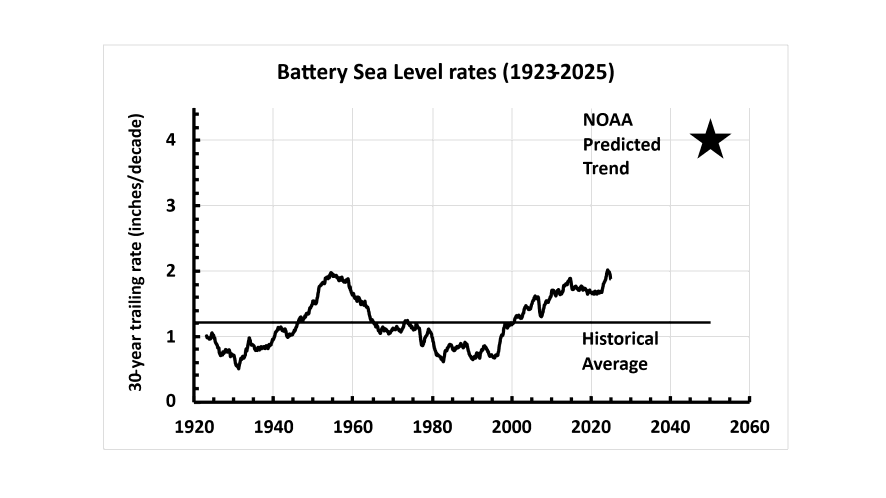
\includegraphics[width=0.9\textwidth]{bilder/bilderKlima-0073.png}\\[1cm]
\end{center}
\caption{Rate des Meeresspiegelanstiegs am Battery in Manhattan. Gezeigt ist der historische dreißigjährige nachlaufende Trend zusammen mit dem angeblich „feststehenden" NOAA-vorhergesagten Trend für 2050. Historische Daten: NOAA Tides and Current.}
\end{figure}

\vfill
\noindent\textbf{Literaturverzeichnis:}

\begingroup
\parindent=0pt
\everypar{\hangindent=2em\hangafter=1\relax}

Fox-Kemper, B., Hewitt, H. T., Xiao, C., Adalgeirsdóttir, G., Drijfhout, S. S., Edwards, T. L., ... \& Yu, Y.
(2021). Ocean, cryosphere and sea level change. In Climate Change 2021: The Physical Science
Basis. Contribution of Working Group I to the Sixth Assessment Report of the Intergovernmental
Panel on Climate Change (pp. 1211–1362). Geneva, Switzerland: Intergovernmental Panel on
Climate Change.

Karegar, M. A., Dixon, T. H., \& Engelhart, S. E. (2016). Subsidence along the Atlantic Coast of North
America: Insights from GPS and late Holocene relative sea level data. Geophysical Research Letters,
43(7), 3126–3133. https://doi.org/10.1002/2016GL068015
80

Kasmarek, M. C., \& Ramage, J. K. (2017). Water-level altitudes 2017 and water-level changes in the
Chicot, Evangeline, and Jasper aquifers and compaction 1973–2016 in the Chicot and Evangeline
aquifers, Houston-Galveston Region, Texas (Scientific Investigations Report 2017–5080). U.S.
Geological Survey. https://doi.org/10.3133/sir20175080

Letetrel, C., Becker, M., Llovel, W., \& Cazenave, A. (2015). Estimation of vertical land movement rates
along the coasts of the Gulf of Mexico over the past decades. Continental Shelf Research, 111(Part
A), 42–51. https://doi.org/10.1016/j.csr.2015.10.018

Maloney, J. M., Bentley, S. J., Xu, K., Obelcz, J., Georgiou, I. Y., \& Miner, M. D. (2018). Mississippi
River subaqueous delta is entering a stage of retrogradation. Marine Geology, 400, 12–23.
https://doi.org/10.1016/j.margeo.2018.03.001

National Academy of Science (NAS, 2012). Sea-level rise for the coasts of California, Oregon and
Washington: Past, present, and future. Appendix A: Vertical land motion and sea-level data along the
West Coast of the United States. National Academies Press.
https://nap.nationalacademies.org/catalog/13389/sea-level-rise-for-the-coasts-of-california-oregon-
and-washington

NASA. (2020). NASA sea level rise portal: 2020 edition. https://www.nasa.gov/specials/sea-level-rise-
2020/

National Oceanic and Atmospheric Administration (NOAA) Center for Operational Oceanographic
Products and Services. (n.d.). Sea level trends. https://tidesandcurrents.noaa.gov/sltrends/

NOAA Tides \& Currents. (n.d.). Relative sea level trends. https://tidesandcurrents.noaa.gov/sltrends/

Nienhuis, J. H., Törnqvist, T. E., Esposito, C. R., Liang, M., \& Ma, H. (2017). A new subsidence map for
coastal Louisiana. GSA Today, 27(6), 28–29. https://doi.org/10.1130/GSATG337GW.1

Shirzaei, M., \& Bürgmann, R. (2018). Global climate change and local land subsidence exacerbate
inundation risk to the San Francisco Bay Area. Science Advances, 4(3), eaap9234.
https://doi.org/10.1126/sciadv.aap9234

Sweet, W. V., Hamlington, B. D., Kopp, R. E., et al. (2022). Global and regional sea level rise scenarios
for the United States (USGS Report 70229139). United States Geological Survey.
https://www.usgs.gov/publications/global-and-regional-sea-level-rise-scenarios-united-states

Wöppelmann, G., \& Marcos, M. (2016). Vertical land motion as a key to understanding sea level change
and variability. Reviews of Geophysics, 54, 64–92. \url{https://doi.org/10.1002/2015RG000502}

\endgroup

\cleardoublepage
\FigureNumbersByChapter 
\chapter{UNSICHERHEITEN IN DER KLIMAWANDEL-ATTRIBUTION}
\paragraph{Kapitelzusammenfassung}
\begin{quote}
\emph{Attribution} bezieht sich auf die Identifizierung der Ursache eines Aspekts des Klimawandels, speziell mit Bezug auf anthropogene Aktivitäten. Es gibt eine anhaltende wissenschaftliche Debatte um Attributionsmethoden, insbesondere bezüglich extremer Wetterereignisse. Attribution wird durch hohe natürliche Variabilität, das relativ kleine erwartete anthropogene Signal, den Mangel an hochwertigen Daten und die Abhängigkeit von mangelhaften Klimamodellen erschwert. Das IPCC hat lange davor gewarnt, dass Methoden zur Etablierung von Kausalität in der Klimawissenschaft inhärent unsicher sind und letztendlich von Expertenbewertung abhängen.

Substanzielle Kritik an den Hauptbewertungen des IPCC zur Rolle von CO$_2$ in der jüngsten Erwärmung konzentriert sich auf unzureichende Bewertung der natürlichen Klimavariabilität, Unsicherheiten in der Messung der solaren Variabilität und des Aerosol-Antriebs sowie Probleme in den statistischen Methoden, die für die Attribution verwendet werden.

Das IPCC macht keine Attributionsansprüche für die meisten klimatischen Einflussfaktoren im Zusammenhang mit Extremereignissen. Aussagen bezüglich der Statistiken globaler Extreme (z.B. Ereigniswahrscheinlichkeit oder Wiederkehrzeiten, Magnitude und Häufigkeit) werden aufgrund von Datenlimitationen allgemein nicht als genau betrachtet und werden mit geringer Zuversicht gemacht. Die Attribution einzelner extremer Wetterereignisse ist aufgrund ihrer Seltenheit herausfordernd.
Widersprüchliche Behauptungen über die Ursachen der Hitzewelle in Westliches Nordamerika 2021 illustrieren die Gefahren hastiger Attributionsbehauptungen über einzelne Extremereignisse.
\end{quote}

\section{Einleitung}
Das Zwischenstaatliche Gremium für Klimaänderungen (IPCC) unterscheidet zwischen der Detektion von Klimawandel und der Attribution seiner Ursache. Wie im AR6 WGI Glossar definiert (IPCC, 2025):

\begin{quote}
\emph{Detektion:} Detektion von Veränderung wird definiert als der Prozess des Nachweises, dass sich das Klima oder ein vom Klima betroffenes System in einem bestimmten statistischen Sinn verändert hat, ohne einen Grund für diese Veränderung zu liefern. Eine identifizierte Veränderung wird in Beobachtungen detektiert, wenn ihre Wahrscheinlichkeit des Auftretens durch Zufall allein aufgrund interner Variabilität als gering bestimmt wird, beispielsweise $<10\%$.

\emph{Attribution:} Attribution wird definiert als der Prozess der Bewertung der relativen Beiträge mehrerer kausaler Faktoren zu einer Veränderung oder einem Ereignis mit einer formalen Bewertung der Zuversicht.
\end{quote}

Sowohl Detektion als auch Attribution beruhen auf statistischer Analyse. Detektion konzentriert sich darauf, ob Veränderungen signifikant genug sind, um sich von zufälliger Variation unabhängig von der Ursache abzuheben. Attribution beinhaltet den Vergleich beobachteter Ereignisse mit modell-generierten kontrafaktischen Szenarien. Da Experimente am Klima nicht möglich sind, erfordert Attribution statistische Inferenz, um zu bewerten, wie sehr menschliche Aktivitäten (wie THG-Emissionen) versus natürliche Faktoren (wie Vulkanausbrüche) zu beobachteten Veränderungen beitragen. Attributionsmethoden nehmen an, dass alle externen und internen Treiber des Systems bekannt und repräsentiert sind.

Es gibt anhaltende wissenschaftliche Debatten um Attributionsmethoden, insbesondere jene zur Attribution extremer Wetterereignisse auf den Klimawandel. Das IPCC hat lange davor gewarnt, dass Methoden zur Etablierung von Kausalität in der Klimawissenschaft inhärent unsicher sind und letztendlich von Expertenbewertung abhängen. AR4 Working Group I (Hegerl et al., 2007) erklärte es folgendermaßen:

\begin{quote}
\emph{Attribution} von Ursachen des Klimawandels ist der Prozess der Etablierung der wahrscheinlichsten Ursachen für die detektierte Veränderung mit einem definierten Niveau der Zuversicht... eindeutige Attribution würde kontrollierte Experimente mit dem Klimasystem erfordern. Da das nicht möglich ist, wird Attribution anthropogenen Klimawandels in der Praxis verstanden als Nachweis, dass eine detektierte Veränderung „konsistent mit den geschätzten Reaktionen auf die gegebene Kombination anthropogener und natürlicher Antriebe" ist und „nicht konsistent mit alternativen, physikalisch plausiblen Erklärungen jüngsten Klimawandels, die wichtige Elemente der gegebenen Kombination von Antrieben ausschließen" (IPCC, 2001)... Die in der Detektions- und Attributionsforschung beschriebenen Ansätze können nicht vollständig alle Unsicherheiten berücksichtigen, und daher ist letztendlich Expertenbewertung erforderlich, um eine kalibrierte Bewertung zu geben, ob eine spezifische Ursache für eine gegebene Klimaveränderung verantwortlich ist.
\end{quote}

AR5 Working Group II (Cramer et al., 2014) macht die folgende Aussage:

\begin{quote}
Zwei breite Herausforderungen für die Detektion und Attribution von Klimawandel-Auswirkungen beziehen sich auf Beobachtungen und Prozessverständnis. Auf der Beobachtungsseite sind hochwertige, langfristige Daten bezüglich natürlicher und menschlicher Systeme und der multiplen Faktoren, die sie beeinflussen, selten. Zusätzlich erfordern die Detektion und Attribution von Klimawandel-Auswirkungen ein Verständnis der Prozesse, durch die Klimawandel in Verbindung mit anderen Faktoren das fragliche System beeinflussen kann. 
\end{quote}

Aufgrund der Komplexität der kausalen Ketten im Klimasystem ist die Untersuchung dieser Beziehungen außerordentlich herausfordernd.


\section{Attributionsmethoden}
Das IPCC verwendet mehrere Attributionsmethoden, um die Ursachen beobachteter Klimaveränderungen zu bewerten und zwischen natürlichen und menschlich induzierten Faktoren zu unterscheiden. Unten ist eine prägnante Beschreibung der wichtigsten IPCC-Attributionsmethoden.

\emph{Optimales Fingerprinting} verwendet lineare Regression, um Variationen in beobachteten Klimadaten als gewichtete Summe von Klimamodellsimulationen zu erklären, die mit und ohne anthropogene Antriebe durchgeführt wurden. Die in dem Regressionsmodell verwendeten Daten werden gewichtet, um zu versuchen, den Einfluss von zufälligem Rauschen zu minimieren, und die Schätzmethode wird gewählt, um Klimamodellfehler zu berücksichtigen.

\emph{Zeitreihenanalyse} nutzt statistische Unterschiede zwischen anthropogenen Antrieben und natürlicher Variabilität, um zu sehen, welche die beobachteten Temperaturen dominiert, und verwendet auch Variationen im Timing von Veränderungen, um zu bestimmen, ob kausale Abhängigkeit zwischen Datenreihen abgeleitet werden kann.

\emph{Prozessbasierte Attribution} konzentriert sich auf das Verständnis der physikalischen Mechanismen hinter beobachteten Veränderungen. Dieser Ansatz kombiniert Beobachtungen, Klimamodelle und theoretisches Verständnis, um Veränderungen in spezifischen Prozessen Antrieben zuzuordnen. Dieser Ansatz wird oft für regionale Klimaphänomene verwendet, wie Monsoonveränderungen oder polare Verstärkung.

\emph{Extreme Event Attribution} bewertet die Rolle menschlichen Einflusses auf die Wahrscheinlichkeit des Auftretens oder die Intensität extremer Wetterereignisse (z.B. Hitzewellen oder Dürren). Methoden umfassen:

\begin{itemize}
\item Probabilistische Ereignis-Attribution verwendet große Ensembles von Klimamodellsimulationen, um beobachtete Ereignisse mit modell-generierten kontrafaktischen Szenarien zu vergleichen
\item Storyline-Ansatz untersucht die physikalischen Prozesse, die ein Ereignis antreiben, und bewertet, wie anthropogene Antriebe diese Prozesse modifiziert haben könnten
\end{itemize}

\section{Attribution der globalen Erwärmung}
Attributionsaussagen für die globale Erwärmung in den drei jüngsten IPCC-Bewertungsberichten sind:

\begin{quote}
\emph{AR4:} \textbf{Der größte Teil des beobachteten Anstiegs} der global gemittelten Temperaturen seit der Mitte des 20. Jahrhunderts ist sehr wahrscheinlich auf den beobachteten Anstieg der anthropogenen Treibhausgaskonzentrationen zurückzuführen. (IPCC 2007)

\emph{AR5:} Es ist extrem wahrscheinlich, dass \textbf{mehr als die Hälfte des beobachteten Anstiegs} der global gemittelten Oberflächentemperatur von 1951 bis 2010 durch den anthropogenen Anstieg der Treibhausgaskonzentrationen und andere anthropogene Antriebe zusammen verursacht wurde. Die beste Schätzung des menschlich induzierten Beitrags zur Erwärmung ist ähnlich der beobachteten Erwärmung über diesen Zeitraum. (IPCC 2013)

\emph{AR6:} Der wahrscheinliche Bereich des gesamten menschlich verursachten globalen Oberflächentemperaturanstiegs von 1850–1900 bis 2010–2019 liegt zwischen 0,8°C und 1,3°C, mit einer besten Schätzung von 1,07°C. Es ist wahrscheinlich, dass gut durchmischte THGs eine Erwärmung von 1,0°C bis 2,0°C beigetragen haben, andere menschliche Treiber (hauptsächlich Aerosole) eine Abkühlung von 0,0°C bis 0,8°C beigetragen haben, natürliche Treiber die globale Oberflächentemperatur um –0,1°C bis +0,1°C verändert haben und interne Variabilität sie um –0,2°C bis +0,2°C verändert hat. Es ist sehr wahrscheinlich, dass \textbf{gut durchmischte THGs der Haupttreiber der troposphärischen Erwärmung} seit 1979 waren. (IPCC 2021)
\end{quote}

Die AR4- und AR5-Attributionsaussagen beziehen sich auf die Erwärmung seit Mitte des 20. Jahrhunderts, dem Zeitraum, als Treibhausgasemissionen zu steigen begannen. Die Worte \emph{größter Teil} und \emph{mehr als die Hälfte} sind bewusst ungenau und reichen potenziell von 51 bis 99 Prozent der Erwärmung – vermutlich ist diese Ungenauigkeit dazu da, strukturelle Unsicherheiten wie natürliche interne Variabilität zu berücksichtigen. Das Konfidenzniveau steigt von sehr wahrscheinlich zu extrem wahrscheinlich von AR4 zu AR5. Die Struktur der Attributionsaussage in AR6 ist grundlegend anders und bezieht sich auf die Erwärmung zum Zeitraum 1850-1900. Die AR6-Attributionsaussage ist numerisch präziser, aber mit einem niedrigeren Konfidenzniveau bei \emph{wahrscheinlich} – AR6 attribuiert im Wesentlichen die gesamte Erwärmung auf Treibhausgasanstiege. Die konfidenteste Aussage von AR6 bezieht sich auf die troposphärische Erwärmung seit 1979, mit den Worten \emph{Haupttreiber} und \emph{sehr wahrscheinlich}.

Es gibt drei Bereiche substanzieller Kritik an der IPCC-Bewertung der Ursachen der jüngsten Erwärmung: unzureichende Bewertung der natürlichen Klimavariabilität, ungeeignete statistische Methoden und substantielle Diskrepanzen zwischen Modellen und Beobachtungen. Letzteres wird in Kapitel 5 diskutiert, während dieses Kapitel die ersten beiden Faktoren diskutiert. Alle diese Kritikpunkte sind relevant für die IPCC-Attribution der jüngsten Erwärmung, die auch der Grundlage der Attribution extremer Ereignisse zugrunde liegt.


\subsection{Natürliche Klimavariabilität}
AR6 stellt fest, dass natürliche externe Treiber seit 1850-1900 die globale Oberflächentemperatur um –\SI{0.1}{\celsius} bis \SI{+0.1}{\celsius} verändert haben und interne Variabilität sie um –\SI{0.2}{\celsius} bis \SI{+0.2}{\celsius} verändert hat – im Durchschnitt haben sie im Wesentlichen keinen Nettoeinfluss auf die Erwärmung seit 1850-1900. Wie unten diskutiert, wurde dieser minimale Beitrag natürlicher Variabilität von mehreren Veröffentlichungen bestritten, die die Größenordnungen solarer Variabilität und interner Variabilität aus großskaligen Ozeanzirkulationen in Frage stellen.

\emph{Solare Variabilität}

AR5 kam zu dem Schluss, dass die beste Schätzung des Strahlungsantriebs durch Änderungen der Gesamtsonnenbestrahlung (Total Solar Irradiance, TSI) über den Zeitraum 1750–2011 sehr klein war ($0.05$ \si{\watt\per\square\meter}, Myrhe et al., 2014). AR6 erkennt substantiell höhere Werte und eine viel größere Bandbreite von Schätzungen der TSI-Änderungen über die letzten mehreren Jahrhunderte an und stellt fest, dass die TSI zwischen dem Maunder-Minimum (1645–1715) und der zweiten Hälfte des zwanzigsten Jahrhunderts um $0.7 - 2.7$ \si{\watt\per\square\meter} anstieg, eine Bandbreite, die sowohl niedrige als auch hohe TSI-Variabilitätsdatensätze umfasst (Gulev, 2021). Jedoch mittelt der für die CMIP6-Klimamodellsimulationen empfohlene Antriebsdatensatz, der in AR6 für Attributionsstudien verwendet wird, zwei Datensätze mit niedriger solarer Variabilität (Matthes, 2017).

Während AR6 einen substantiell größeren solaren Einfluss zeigt als AR5, wurde der Gesamteinfluss solaren Antriebs auf das Klima dennoch als klein im Vergleich zu anthropogenem Antrieb bewertet. Jedoch ist der Einfluss solarer Variationen auf das Klima unsicher und Gegenstand substanzieller Debatte (Lockwood, 2012; Connolly et al., 2021) – etwas, das in den IPCC-Bewertungsberichten nicht evident ist.

Die Variationen der TSI über die Zeit bleiben ein herausforderndes Problem. Seit 1978 gibt es direkte Messungen der TSI von Satelliten. Jedoch zeigen die Daten nicht vernachlässigbare Inkonsistenzen, und die Interpretation multidekadenaler Trends in der TSI erfordert Vergleiche von Beobachtungen überlappender Satelliten. Es gibt mehrere rivalisierende zusammengesetzte TSI-Datensätze, die darüber uneinig sind, ob die TSI während des Zeitraums 1986–96 anstieg oder abnahm (die ACRIM-Lücke; siehe Kapitel 4). Weiterhin wird die Satellitenaufzeichnung der TSI verwendet, um Proxy-Modelle zu kalibrieren, die vergangene solare Variationen aus Sonnenflecken- und kosmogenen Isotopenmessungen ableiten (Velasco Herrera et al., 2015).

Es gibt substanzielle Belege für hohe Sonnenaktivität in der zweiten Hälfte des 20. Jahrhunderts (beginnend 1959) und sich bis in die 1990er erstreckend, vor einem Rückgang im frühen 21. Jahrhundert; dieser Zeitraum wird oft als „Modernes Maximum" bezeichnet (Chatzistergos et al., 2023; Solanki et al., 2004; Usoskin et al., 2007). Jedoch haben einige Wissenschaftler geschlossen, dass es nicht möglich ist, bezüglich eines multidekadenalen Trends in der TSI zuversichtlich zu sein (Schmutz, 2021).

Diese Unsicherheit verursacht, dass einige Rekonstruktionen der TSI ab 1750 niedrige Variabilität haben (was einen sehr niedrigen Einfluss solarer Variationen auf die globale mittlere Oberflächentemperatur impliziert), während Datensätze mit hoher TSI-Variabilität mehr als 70 Prozent der Temperaturvariabilität seit vorindustriellen Zeiten erklären können (Scafetta, 2013; Stefani, 2021). Die Wahl der TSI-Satellitenaufzeichnung, die in einer Analyse verwendet wird, kann daher substantiell beeinflussen, wie viel Klimawandel menschlichen versus natürlichen Antrieben zugeschrieben wird.

Es gibt wachsende Belege, dass andere Aspekte solarer Variabilität, die als solare indirekte Effekte bezeichnet werden, entweder TSI-Antrieb verstärken oder unabhängig von TSI-Antrieb sind. Scafetta et al. (2023) suggerieren, dass ~80 Prozent des solaren Einflusses auf das Klima von Nicht-TSI-Mechanismen herrühren könnten. Es gibt zahlreiche Kandidatenprozesse, einschließlich solarer Ultraviolett-Änderungen; energetischer Teilchenniederschlag; atmosphärisch-elektrischer Feldeffekt auf Wolkenbedeckung; Wolkenveränderungen, die durch solar-modulierte galaktische kosmische Strahlung produziert werden; große relative Änderungen im Magnetfeld; und die Stärke des Sonnenwinds. Solche solaren indirekten Effekte sind nicht in Klimamodellen enthalten, obwohl indirekte Methoden zur Schätzung ihrer Einflüsse suggerieren, dass sie signifikant sind. Jedoch sind Behauptungen von Nicht-TSI-Mechanismen, die das Klima beeinflussen, unsicher und umstritten.

\textbf{Natürliche Variabilität großskaliger Ozeanzirkulationen}

Variationen der globalen mittleren Oberflächentemperatur sind verknüpft mit wiederkehrenden großskaligen Variationen in Ozeanzirkulationsmustern, einschließlich der Atlantischen Multidekadenoszillation (AMO), der Pazifischen Dekadenoszillation (PDO) und der El Niño-Southern Oszillation (ENSO). Diese Zirkulationen beeinflussen die ozeanische Wärmeaufnahme und Wärmeverteilung und beeinflussen auch atmosphärische Zirkulationsmuster und Wolkenverteilungen. Es gibt einige Debatten darüber, ob diese Variationen strikt intern zum Klimasystem sind oder ob diese Variabilität einen solaren/astronomischen Ursprung haben kann oder durch große Vulkanausbrüche beeinflusst werden kann.

Während Klimamodelle die großskaligen Ozeanzirkulationen und interne Klimavariabilität simulieren, haben die meisten Modelle zu wenig Amplitude im Vergleich zu Beobachtungen bei multidekadenalen Frequenzen und eine Phasenverschiebung außer Takt mit dem beobachteten Klima (Kravtsov et al. 2024). Die Mittelung multipler Simulationen mittelt effektiv die internen Variationen heraus und lässt nur die erzwungene Klimavariabilität übrig (z.B. CO$_2$-Antrieb). Da der größte Teil der modernen Erwärmung in den späten 1970ern begann, liegt die jüngste 50-Jahre-Erwärmung auf derselben Zeitskala wie die multidekadenalen Oszillationen der AMO und PDO.

Hier sind zusammenfassende Aussagen aus den AR5- und AR6-Berichten:

\begin{quote}
AR5: Dekadenale Variabilität im Pazifik, verbunden mit der PDO oder IPO [Interdekadische Pazifische Oszillation], trägt signifikant zu regionalen und globalen Temperaturtrends bei, aber die relativen Beiträge interner Variabilität und externen Antriebs sind schwierig in CMIP5-Simulationen zu entwirren.

AR6: Seit AR5 gab es ein verstärktes Verständnis der Rolle interner Variabilität, wie ENSO, PDO und AMO, bei der Modulation regionaler Klimatrends. Jedoch tragen Limitationen bei der Simulation des exakten Timings und der Amplitude dieser Modi in CMIP6-Modellen zu Unsicherheiten bei der Attribution beobachteter Veränderungen auf anthropogenen Antrieb bei (\emph{hohe Zuversicht}).
\end{quote}

Die Amplitude der Peak-zu-Tal-Auswirkung der multidekadenalen Oszillationen auf globale Temperaturen wurde vom IPCC AR6 bewertet: „Der wahrscheinliche Bereich der Veränderung aufgrund interner Variabilität ist -0,2°C bis +0,2°C (IPCC, 2021)." Dies impliziert eine Tal-zu-Peak-Veränderung von 0,4°C. Über viele Jahrhunderte werden sich alle globalen Temperaturveränderungen von den Tälern und Peaks ausgleichen, mit wenig bis keinem Nettoeinfluss.

Jedoch kann mit einem nominalen Zeitrahmen von 60-80 Jahren für Oszillationen wie AMO und PDO das Timing der Peaks und Täler mit dem säkularen Trend verwechselt werden. Dies wird sehr relevant für die Attribution der Erwärmung der letzten 50 Jahre, als der größte Teil der jüngsten Erwärmung aufgetreten ist. Selbst wenn Klimamodelle die korrekte Amplitude der multidekadenalen Oszillationen haben, wird das Timing der Peaks und Täler nicht angemessen simuliert, wobei jedes Modell und individuelle Ensemble eine unterschiedliche Phasenverschiebung simuliert. Sobald die Simulationen der Ensemble-Mitglieder und verschiedenen Modelle gemittelt werden, wird der Beitrag natürlicher interner Variabilität aufgrund von Unterschieden in der Phasenverschiebung herausgemittelt, wodurch die Rolle natürlicher interner Variabilität im Attributionsprozess effektiv aufgehoben wird.

Die Zeitreihe der globalen Oberflächentemperaturanomalien seit 1850 (Abbildung 8.1) zeigt unregelmäßige Variationen signifikanter Amplitude vor dem Hintergrund eines allgemeinen Erwärmungstrends und, nach 1976, einen ausgeprägten Unterschied in Trends zwischen der nördlichen und südlichen Hemisphäre. Der Zeitraum zwischen 1905-1945 zeigt einen starken Erwärmungstrend. Die folgenden 30 Jahre von 1945-1976 zeigten leicht rückläufige Temperaturen. Der jüngste Erwärmungszeitraum begann 1977.

\begin{figure}[H]
\begin{center}
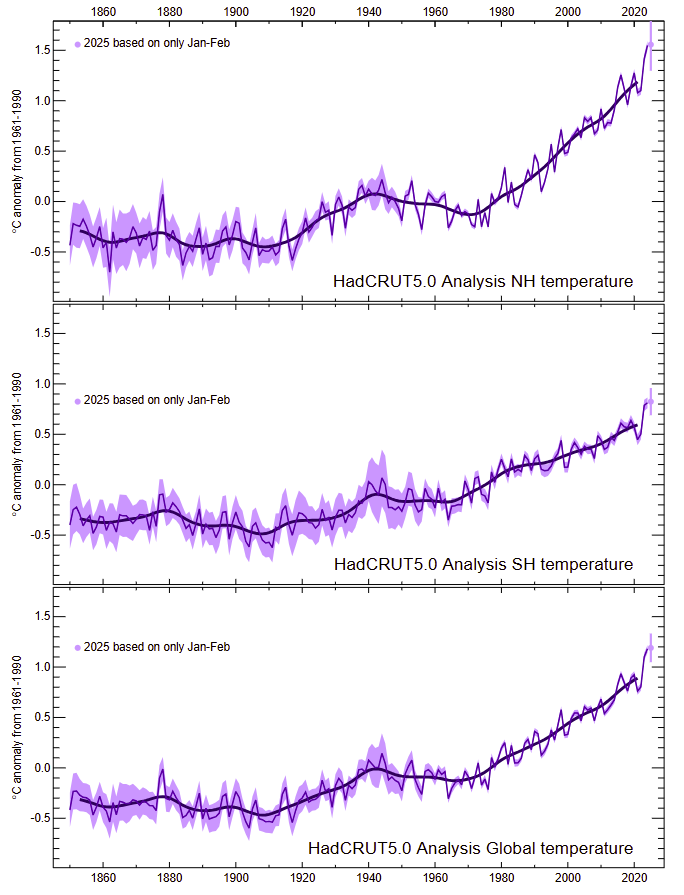
\includegraphics[width=0.9\textwidth]{bilder/bilderKlima-0074.png}\\[1cm]
\end{center}
\caption{Globale durchschnittliche Oberflächentemperaturanomalien 1850—2025. Oben: Nördliche Hemisphäre. Mitte: Südliche Hemisphäre. Unten: Globaler Durchschnitt. Quelle: UK Hadley Centre https://crudata.uea.ac.uk/cru/data/temperature/HadCRUT5.0Analysis.pdf}
\end{figure}

Die Ursachen der frühen Erwärmung des 20. Jahrhunderts werden von Hegerl et al. (2017; 2019) diskutiert. Die atmosphärische CO$_2$-Konzentration stieg von \SI{298}{ppm} in 1905 auf \SI{310}{ppm} in 1941, was impliziert, dass CO$_2$ wenig Einfluss hatte. Vulkanaktivität während dieses Zeitraums war sehr niedrig, und solarer Antrieb ist unsicher. Dennoch schlossen Hegerl et al. (2017) irgendwie, dass 40-54 Prozent dieser Erwärmung externen Antrieben zugeschrieben werden könnte, wobei der Rest mit interner Variabilität verbunden war. Bronniman et al. (2024) konzentrierten sich auf die Ursachen der Abkühlung in dem ersten Jahrzehnt des 20. Jahrhunderts in der südlichen Hemisphäre. Sie fanden, dass die Abkühlung mit einem La-Niña-ähnlichen Muster im Pazifik, einem kalten tropischen und subtropischen Südatlantik, einem kalten extratropischen Südpazifik und kühlen südlichen mittleren Breitengradlandgebieten verbunden war. Der Southern Annular Mode war positiv, mit einem verstärkten Amundsen–Bellingshausen-Meere-Tief, obwohl die Streuung der Datenprodukte beträchtlich ist.

Die Erwärmung in den 1930ern und nachfolgende Abkühlung während der Jahrhundertmitte war besonders ausgeprägt in der Arktis. Bokuchava und Semenov (2021) finden, dass diese Variationen höchstwahrscheinlich durch einen kombinierten Effekt langfristiger natürlicher Klimavariationen im Nordatlantik und Nordpazifik mit einem Beitrag des natürlichen Strahlungsantriebs im Zusammenhang mit der reduzierten Vulkanaktivität und Variationen der Sonnenaktivität sowie wachsenden Treibhausgaskonzentrationen verursacht wurden. Tokinaga et al. (2017) zeigten, dass der kombinierte Effekt intern generierter pazifischer und atlantischer interdekadischer Variabilität die arktische Erwärmung im frühen 20. Jahrhundert verstärkte. Die synchronisierte pazifisch-atlantische Erwärmung verändert drastisch planetarische Zirkulationen über der nördlichen Hemisphäre; diese gleichen Zirkulationsmuster haben einen globalen Einfluss.

Die Abkühlungsperiode zwischen 1945 und 1976 wurde als „großer Hiatus" bezeichnet. Zahlreiche Ursachen wurden als Hypothese aufgestellt: natürliche interne Variabilität von Fluktuationen verbunden mit der Pazifischen Dekadenoszillation und Atlantischen Multidekadenoszillation; Abkühlung durch erhöhte Emissionen von Aerosolen aus industriellen Aktivitäten; erhöhte Wärmeaufnahme im Atlantik, Süd- und Äquatorialen Pazifischen Ozean. Thompson et al. (2010) finden, dass die hemisphärischen Unterschiede in Temperaturtrends in der Mitte des zwanzigsten Jahrhunderts größtenteils von einem rapiden Abfall der Meeresoberflächentemperaturen der nördlichen Hemisphäre um etwa 0,3 °C zwischen etwa 1968 und 1972 herrühren.

Der Great Pacific Climate Shift von 1976-1977 war ein bemerkenswerte klimatisches Ereignis, charakterisiert durch eine abrupte Veränderung im Atmosphären-Ozean-System des Nordpazifiks, das mit globalen Klimamustern interagierte. Diese Verschiebung ist eng verbunden mit der Pazifischen Dekadenoszillation (PDO), die zwischen warmen und kühlen Phasen über Jahrzehnte oszilliert. Die 1976-Verschiebung markierte einen Übergang von einer vorwiegend negativen (kühlen) PDO-Phase (1947–1976) zu einer positiven (warmen) Phase (1977 bis 2000), mit signifikanten Implikationen für globale und regionale Klimamuster, einschließlich der Häufigkeiten von El Niño- und La Niña-Ereignissen. Der Great Pacific Climate Shift fiel zusammen mit dem Beginn einer Periode beschleunigter globaler Erwärmung. Wenn der Great Pacific Climate Shift in Klimaattributionsanalysen seit 1950 berücksichtigt wird, werden 40 Prozent oder mehr der Erwärmung in der zweiten Hälfte des 20. Jahrhunderts natürlicher interner Variabilität zugeschrieben (McLean et al., 2009; Tung und Zhou, 2013; Chylek et al., 2016; Scafetta, 2021).

\subsection{Optimales Fingerprinting}
Optimales Fingerprinting ist eine statistische Technik, die von Allen und Tett (1999) eingeführt wurde, die beobachtete Klimadaten mit Klimamodellsimulationen vergleicht, um Muster (oder „Fingerabdrücke") zu identifizieren, die mit menschlichen oder natürlichen Antrieben verbunden sind. Es beinhaltet die Aufnahme eines Vektors beobachteter Klimaänderungen, wie Erwärmungsraten an Orten rund um die Welt, und deren Zerlegung in eine gewichtete Summe von „Signalen", die Analoga zu den Beobachtungen sind, die von Klimamodellen mit verschiedenen Arten von Antrieben generiert wurden. Die Gewichte werden unter Verwendung einer Regressionsmethode namens Total Least Squares (TLS) gewählt. Die Analyse verwendet gewöhnlich nur zwei Signale, eines generiert von Modellen, die nur anthropogene Antriebe verwenden, und eines, das nur natürliche Antriebe verwendet. Wenn der geschätzte Gewichtungskoeffizient, der an ein Signal angehängt ist, signifikant von null verschieden ist, dann wird gesagt, dass dieses Signal „detektiert" wird. Wenn er nahe bei 1.0 liegt, dann wird gesagt, dass das Modell, das das Signal generiert, konsistent mit Beobachtungen ist. Wenn er weniger als 1.0 ist, dann ist das Modellsignal für diesen Antrieb zu stark und muss herunterskaliert werden, und umgekehrt. Sowohl die beobachteten Daten als auch die Signale werden unter Verwendung einer modell-generierten Schätzung von Mustern der Zufälligkeit im Klimasystem gewichtet, um im Prinzip maximales Gewicht auf Regionen zu legen, wo natürliche Variabilität minimiert ist.

Optimales Fingerprinting ist das primäre Werkzeug für Attribution in der Forschungsliteratur. Während es weit verwendet wurde und prominent vom IPCC seit 2001 hervorgehoben wurde, gibt es sehr wenig Literatur, die die statistischen Eigenschaften der Ergebnisse untersucht, die es generiert. Eine seiner inhärenten Schwächen ist, dass Ergebnisse von Annahmen über die Genauigkeit von Klimamodellen abhängen, besonders bezüglich ihrer Darstellung natürlicher Variabilität (IPCC AR5 Ch 10.2.3).

Eine Serie von Papers von McKitrick (McKitrick 2021, 2022, 2023, 2025) hat die optimale Fingerprinting-Methode herausgefordert, argumentierend, dass sie inhärent unzuverlässig ist und dass Praktiken, die aus der Ökonometrie adoptiert wurden, validere Ergebnisse liefern können. Statistische Theorie erfordert, dass für Regressionsmodelle, um unverzerrte Koeffizienten zu liefern, eine Reihe von Annahmen, die Gauss-Markov-Bedingungen genannt werden, erfüllt sein müssen. McKitrick (2021) argumentierte, dass die Allen und Tett (1999) Methodologie die Gauss-Markov-Bedingungen verletzt, was zu potenziell verzerrten und inkonsistenten Fingerprinting-Koeffizienten führt, wodurch die Zuverlässigkeit der Methode untergraben wird. Chen et al. (2023) bestätigten diese Analyse, obwohl sie argumentierten, dass die Methode valide Ergebnisse unter sehr stringenten Annahmen liefern könnte. McKitrick (2022) und (2023) warfen eine weitere Sorge auf, dass Klimawissenschaftler – praktisch allein unter wissenschaftlichen Disziplinen – TLS verwendet haben, um anthropogene Treibhausgas-Signalkoeffizienten zu schätzen, trotz seiner Tendenz, instabil zu sein, es sei denn, einige starke Annahmen gelten, die in der Praxis unwahrscheinlich wahr sind.
Unter Bedingungen, die leicht im optimalen Fingerprinting auftreten, haben TLS-Schätzungen eine große positive Verzerrung. Daher hat jede Studie, die TLS für optimales Fingerprinting verwendete, ohne ihre Anwendbarkeit im spezifischen Datenkontext zu verifizieren, wahrscheinlich die Attribution übertrieben.

McKitrick (2025) präsentierte ein empirisches Beispiel, das die Ergebnisse des konventionellen optimalen Fingerprinting gegen Methoden vergleicht, die aus der Mainstream-Ökonometrie gezogen wurden, die bekanntermaßen für die spezifische Anwendung der Signaldetektion valid sind. Während die IPCC optimale Fingerprinting-Methode einen anthropogenen Signalkoeffizienten nahe 1.0 auf einem globalen Temperaturdatensatz von 1900 bis 2010 liefert, liefert die konsistente Methode einen Koeffizienten um 0.4, der auf etwa 0.65 auf Daten von 1980 bis 2010 ansteigt, was impliziert, dass die Modellreaktion auf Treibhausgase um etwa die Hälfte herunterskaliert werden muss, um optimal zu den Beobachtungen zu passen. Der natürliche Antriebssignalkoeffizient ist im Gegensatz dazu zwischen 2.0 und 4.0, was impliziert, dass die Klimamodellsignale natürlichen Antriebs um das Zwei- bis Vierfache hochskaliert werden müssen, um den beobachteten Klimawandel zu treffen.
Die Fingerprinting-Koeffizienten, die in McKitrick (2025) geschätzt wurden, implizieren, wenn sie verwendet werden, um die durchschnittliche Sensitivität der Klimamodelle zu skalieren, die verwendet wurden, um die Antriebssignale in seinem Datensatz zu generieren, eine Transient Climate Sensitivity von \SI{1.4}{\celsius}, was konsistent mit der Schätzung von Lewis (2023) unter Verwendung einer verschiedenen Schätzmethode und multipler unabhängiger Datensätze ist.

Diese Befunde zeigen an, dass die Grundlage, auf der die optimale Fingerprinting-Methode lange als zuverlässig angesehen wurde, nicht valid ist. Eine individuelle Neuuntersuchung vorheriger Ergebnisse wäre erforderlich, um zu bestimmen, welche Befunde statistisch robust sind.

\subsection{Zeitreihen-Methoden}
Das IPCC (AR5 WGI 10.2.2) lenkte Aufmerksamkeit auf alternative Ansätze zur Bewertung von Kausalität, die aus der Zeitreihen-Ökonometrie-Literatur hervorgingen. Diese haben den Vorteil, nicht von Annahmen über die Genauigkeit von Klimamodellen abzuhängen, aber den Nachteil, dass sie von schwer zu testenden Annahmen über den datengenerierenden Prozess abhängen, der Klima- und Antriebsdaten zugrunde liegt. Die Methoden, die jetzt als Klimaökonometrie bezeichnet werden, verwenden die Werkzeuge der Unit-Root-Tests, Granger-Kausalität und Kointegrations-Analyse, die alle in der Wirtschafts- und Finanzwissenschaft vertraut sind und die langsam in der Klimawissenschaft adoptiert werden. Zeitreihen-Analysemethoden bieten die Möglichkeit zu bestimmen, ob anthropogene oder natürliche Antriebe die primären Treiber des Klimawandels sind, ohne die Verwendung von Klimamodellen zu erfordern, obwohl Schlüsselfragen unentschieden bleiben (z.B. Dergiades et al., 2016, Balcombe et al., 2019, Dagsvik et al., 2020, Razzak, 2022, Dagsvik und Moen, 2023).

\emph{Granger-Kausalität}-Modellierung ist ein Werkzeug zur Bestimmung von Einflussrichtungen in Datenreihen, die sich zusammen bewegen. Es ist ein statistisches, nicht ein physikalisches Konzept. Wenn die Kenntnis des aktuellen Werts einer Variablen die Vorhersagegenauigkeit einer anderen Variablen signifikant verbessert, können wir ableiten, dass eine kausale Verbindung existiert; dies wird Granger-Kausalität genannt. Die Modellierungswerkzeuge, Vektorautoregression genannt, messen direkte Impuls-Antwort-Muster und Rückkopplungen. Eine Anwendung auf die wohlbekannten Vostok-Eiskern-Daten enthüllte einen Fehler in Al Gores Dokumentarfilm Eine unbequeme Wahrheit. Gore zeigte die Daten und lenkte Aufmerksamkeit auf die Kohärenz von Temperatur- und CO$_2$-Änderungen über eine 440.000-Jahre-Spanne, was er behauptete, sei auf CO$_2$ zurückzuführen, das Temperaturänderungen antreibt. Aber Temperaturänderungen können auch atmosphärische CO$_2$-Werte beeinflussen. Davidson et al. (2015) untersuchten die Reihen und fanden, dass Temperatur Granger-verursacht CO$_2$, aber nicht umgekehrt. Mit anderen Worten, auf den Zeitskalen, die in den Vostok-Daten repräsentiert sind, ist die Kohärenz in den Reihen primär auf den Einfluss von Temperatur auf CO$_2$-Werte zurückzuführen, nicht auf die Rückkopplung von CO$_2$-Werten auf Temperatur.

Zusammenfassend sind die primären statistischen Methoden zur Attribution von Kausalität in Klimadaten optimales Fingerprinting und Zeitreihen-Analyse. Anwendungen der Allen und Tett (1999) optimalen Fingerprinting-Methode dominieren die Attributions-Literatur und haben vergangene IPCC-Schlussfolgerungen untermauert, aber Ergebnisse hängen von der Genauigkeit von Klimamodellen ab und die Methode wurde kürzlich als inhärent verzerrt kritisiert. Zeitreihen-Methoden hängen nicht von Klimamodellen ab, erfordern aber ihre eigenen Annahmen und haben Ergebnisse generiert, die bisher nicht zu einem Konsens konvergiert sind.

\section{Abnehmende planetare Albedo und jüngste Rekordwärme}
Ein scharfer jüngster Anstieg der globalen Durchschnittstemperaturen hat die Frage nach kurzfristigen Treibern des Klimas aufgeworfen. Ein solcher Kandidat ist der Anteil der absorbierten Sonnenstrahlung, der in den letzten Jahren ebenfalls abrupt angestiegen ist. Die Frage ist, ob die Änderung eine interne Rückkopplung zur durch Treibhausgase verursachten Erwärmung ist oder ob etwas anderes den Anteil der absorbierten Strahlung erhöhte, was dann die jüngste Erwärmung verursachte.

Die planetare Albedo ist der Anteil der einkommenden Sonnenstrahlung, der zurück in den Weltraum reflektiert wird, anstatt vom Planeten absorbiert zu werden. Hoch reflektierende Oberflächen wie Wolkendecken sowie Schnee und Eis sind in dieser Hinsicht am wichtigsten. Die Albedo der Erde beträgt etwa 30 Prozent, was bedeutet, dass fast ein Drittel des Sonnenlichts, das die Erde erreicht, direkt zurück in den Weltraum reflektiert wird. Eine niedrigere Albedo impliziert, dass mehr Sonnenenergie vom Planeten absorbiert wird, um dann als Wärme abgestrahlt zu werden. Daher ist, unter sonst gleichen Bedingungen, ein Rückgang der planetaren Albedo mit einer Erwärmung der Erde verbunden.

Wohl die auffälligste Änderung im Klimasystem der Erde während des 21. Jahrhunderts ist eine signifikante Reduktion der planetaren Albedo seit 2015, die mit mindestens zwei Jahren rekordhoher globaler Wärme zusammenfiel. Abbildung 8.2 zeigt die planetaren Albedo-Variationen seit 2000, als es gute Satellitenbeobachtungen gab. Die 0,5 Prozent Reduktion der planetaren Albedo seit 2015 entspricht einem Anstieg von 1,7 \si{\watt\per\square\meter} in absorbierter Sonnenstrahlung, gemittelt über den Planeten (Hansen und Karecha, 2025). Zum Vergleich schätzen Forster et al. (2024), dass der aktuelle Antrieb durch den Anstieg des atmosphärischen CO$_2$ im Vergleich zu vorindustriellen Zeiten 2,33 \si{\watt\per\square\meter} beträgt.

Mit einem Rückblick vor 2000 mit weniger angemessenen Daten bewerteten Goessling et al. (2025), dass die planetare Albedo relativ niedrig um die 1940er und 50er Jahre war, bevor steigende industrielle Aerosol-Vorläufer-Emissionen die Albedo bis in die 1980er Jahre erhöhten. Die stärksten planetaren Albedo-Exkursionen waren hohe Albedo-Episoden, die durch Vulkanausbrüche verursacht wurden, wie nach dem Mount Pinatubo-Ausbruch 1991. Obwohl unsicher, könnte das planetare Albedo-Minimum 2023 das niedrigste seit mindestens 1940 gewesen sein.

Änderungen in Oberflächencharakteristika können diese Abnahme der planetaren Albedo seit 2015 nicht erklären:

\begin{itemize}
\item Die arktische Meereisausdehnung ist seit 1980 um etwa 5 Prozent zurückgegangen (\url{https://nsidc.org/data/seaice_index/images/s_plot_hires.png}), obwohl nach 2007 eine Pause im arktischen Meereis-Rückgang aufgetreten ist (England et al., 2025) 
\item Bezüglich antarktischen Meereises schließt das IPCC AR6: \emph{Es gab keinen signifikanten Trend in der antarktischen Meeseisfläche von 1979 bis 2020 aufgrund regional entgegengesetzter Trends und großer interner Variabilität.} (Summary for Policymakers, A.1.5) 
\item Die jährliche Schneebedeckung der nördlichen Hemisphäre ist seit 1967 langsam rückläufig, mit kaum signifikanten Trends. Die Daten zeigen, dass die nördliche Hemisphäre schneereiche Winter hat, begleitet von rascherem Schmelzen im Frühjahr und Sommer, siehe \url{http://climate.rutgers.edu/snowcover/ und Abschnitt 5.6} 
\item Globale Ergrünung (Kapitel 2) trägt zur Abnahme der planetaren Albedo bei, da Wälder eine niedrigere Albedo haben als offenes Land oder Schnee. Jedoch gibt es einige Belege, dass Wälder die Wolkenbedeckung erhöhen (hohe Reflektivität), was der direkten Albedo-Abnahme entgegenwirkt, die mit zunehmender bewaldeter Fläche verbunden ist. 
\end{itemize}

\begin{figure}[H]
\begin{center}
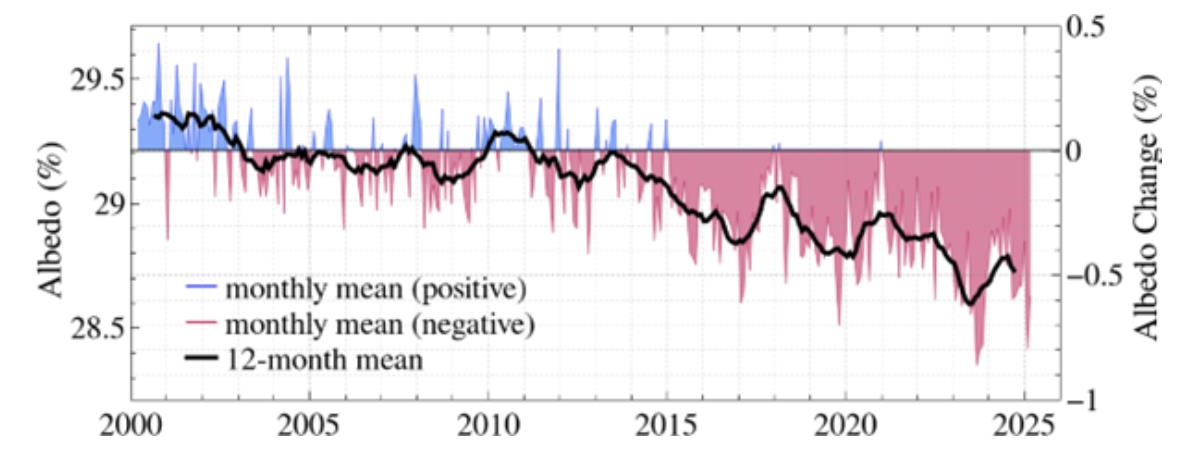
\includegraphics[width=0.9\textwidth]{bilder/bilderKlima-0075.jpg}\\[1cm]
\end{center}
\caption{Albedo der Erde (Reflektivität, in Prozent), mit entfernter Saisonalität. Aus Hansen und Karecha (2025)}
\end{figure}

Änderungen in der Oberflächenreflektivität tragen zu einer kleinen, langsamen Abnahme der planetaren Albedo bei. Jedoch können diese Änderungen die scharfe Abnahme der planetaren Albedo seit 2015 nicht erklären. Weiterhin werden alle Änderungen in der Oberflächenalbedo effektiv um etwa einen Faktor drei im Durchschnitt gedämpft, hauptsächlich aufgrund von Wolkenabdeckung (Loeb et al. 2019). Oberflächenalbedo-Änderungen haben daher nur schwach zur jüngsten planetaren Albedo-Abnahme beigetragen, besonders wenn jährlich und global gemittelt. Das lässt die wahrscheinlichste Erklärung für die scharfe Albedo-Abnahme als Änderungen in atmosphärischen Aerosolen und/oder Wolken.

Aerosole sind kleine Partikel in der Atmosphäre, die Sonnenlicht reflektieren und mit Wolkenprozessen interagieren können, um die Wolken reflektiver zu machen. Aerosole haben sowohl natürliche Ursprünge (z.B. Staub von Böden, Waldbrände) als auch menschliche Ursprünge aus Verbrennung (einschließlich fossiler Brennstoffe). Regionen, die sich begrünen und/oder einen Anstieg der Niederschläge haben, könnten weniger Staub produzieren. Für anthropogene Aerosole wurden neue Schiffstreibstoff-Regulierungen zur Reduzierung von Schwefelemissionen in drei Phasen implementiert: 2010, 2015 und 2020. Sulfat-Partikel reflektieren Sonnenstrahlung, so bedeutet sauberere Luft, dass weniger Sonnenstrahlung reflektiert wird, was zur Oberflächenerwärmung beiträgt. Indirekte Effekte von Sulfat-Aerosolen umfassen die Erhöhung der Reflektivität niedrigstufiger Wolken in den Subtropen. Es gibt Kontroversen um die Wichtigkeit dieser Änderung in Sulfat-Emissionen für die Strahlungsbilanz der Erde (Hodnebrog et al., 2024; Yuan et al., 2024), aber die Beschränkung dieses Effekts auf Hauptschifffahrtsrouten suggeriert einen kleinen globalen Einfluss (Schmidt, 2024).

Änderungen in Wolken sind der primäre Kandidat, um die Abnahme der globalen Albedo seit 2015 zu erklären. Zwei jüngste Papers (Loeb et al., 2024; Goessling et al 2024) haben jüngste Variationen in Wolkeneigenschaften adressiert. Durch Betrachtung von Satelliten- und Reanalyse-Daten fanden Loeb et al., dass Abnahmen in niedrig- und mittelstufigen Wolken seit 2015 der primäre Grund für abnehmende planetare Albedo in der nördlichen Hemisphäre sind, während in der südlichen Hemisphäre die Abnahme in planetarer Albedo primär auf Abnahmen in mittelstufigen Wolken über alle Breitengradzonen zurückzuführen ist. Goessling et al. (2024) fanden, dass Wolkenanomalien hauptsächlich auf reduzierte niedrigstufige Wolken zurückzuführen waren. Regionen mit kohärenten niedrigstufigen Wolken-Reduktionen über das vergangene Jahrzehnt umfassen die warme Pool-Region um den Maritimen Kontinent und den nördlichen extratropischen westlichen Pazifik sowie große Teile des Atlantiks und angrenzender Landregionen. Die Reduktion der globalen Wolkenbedeckung, die in diesen Analysen seit 2015 identifiziert wurde, beträgt 1-2 Prozent.

Die Frage wird dann zur Ursache der Änderung in Wolkenbedeckung. Zwei Erklärungen sind für die abnehmende Wolkenbedeckung über das vergangene Jahrzehnt vorgeschlagen worden:

\begin{itemize}
\item Natürliche Klimavariabilität 
\item Änderungen in niedriger Wolkenbedeckung verbunden mit sich erwärmenden Meeresoberflächentemperaturen, was eine aufkommende positive Rückkopplung zum Klimawandel impliziert (Hansen und Karecha, 2025)
 
\end{itemize}

Es ist nicht einfach, eine neue positive niedrige Wolken-Rückkopplung zu rechtfertigen, die 2015 zu entstehen begann, da es keinen offensichtlichen Rückkopplungsauslöser gibt, der zu dieser Zeit beginnt. Jedoch gibt es zahlreiche natürliche Klimasignale während dieser Periode, die mit atmosphärischen Zirkulationsänderungen verbunden sind, die die Verteilung von Wolken beeinflussen können:

\begin{itemize}
\item Das 2014-2016 war eines der stärksten El Niño-Ereignisse der Aufzeichnungen 
\item Eine kalte Anomalie beginnend 2015 im subpolaren Wirbel des Nordatlantiks reflektiert eine Verschiebung im Ozeanzirkulationsmuster verbunden mit dekadischer Variabilität im Atlantik (Frajka-Williams et al., 2017; Arthun et al. 2021). 
\item Der Pacific Decadal Oscillation positive Index erreichte 2016 seinen Höhepunkt, nahm dann ab und ist seit Ende 2019 in negativem Territorium 
\item Eruption des submarinen Hunga-Tonga Vulkans in 2022 
\end{itemize}


Interannuelle Wolkenanomalien verbunden mit der El Niño Southern Oscillation (ENSO) haben ein signifikantes globales Signal und starke regionale Signale, besonders über den tropischen Indischen und Pazifischen Ozeanen.

Die Hunga Tonga-Eruption ist bemerkenswert in ihrem Zusammenfallen mit dem außergewöhnlich niedrigen Wert planetarer Albedo in 2023. Goessling et al. (2024) fanden, dass die Wolkenstörungen in 2023 ein anderes Muster zeigten als das Gesamtmuster seit 2015, wobei reduzierte Wolkenbedeckung am ausgeprägtesten in der nördlichen Hemisphäre und den Tropen war. Regionale Reduktionen in Wolkenbedeckung waren am ausgeprägtesten über dem östlichen Indischen Ozean, über Südamerika und sich erstreckend über den östlichen Pazifik, sowie über dem nördlichen Nordamerika, im Südlichen Ozean um 60S, im subtropischen und östlichen Nordatlantik und in Teilen des Nordpazifiks.

Die Hunga Tonga-Eruption war ungewöhnlich darin, dass sie große Mengen Wasserdampf in die Stratosphäre injizierte zusätzlich zu Sulfat-Partikeln. Frühe Veröffentlichungen konzentrierten sich auf die Auswirkungen auf stratosphärische Zirkulationen und den direkten Strahlungseffekt. In 2025 erscheinen Papers, die die indirekten Effekte von Hunga Tonga auf Oberflächenklima unter Verwendung von Ensemble-Simulationen aus Erdsystemmodellen untersuchen (Bednarz et al., 2025; Kuchar et al., 2025). Diese Papers fanden statistisch signifikante Auswirkungen auf regionale Klimate, die durch Zirkulationsänderungen von Kopplungen zwischen der Stratosphäre und Troposphäre angetrieben wurden. Diese Papers zeigen die komplexen Interaktionen zwischen vulkanischer Aktivität und Klimadynamik an. Mehr Forschung ist nötig, um alle Auswirkungen der Hunga Tonga-Eruption auf die planetare Albedo zu entwirren.

Zusammenfassend haben die Abnahme der planetaren Albedo und die begleitende Abnahme der Bewölkung die Wichtigkeit von Wolken und ihren Variationen für globale Klimavariabilität und -änderung betont. Eine Änderung von 1-2 Prozent in globaler Wolkenbedeckung hat einen größeren Strahlungseffekt auf das Klima als der direkte Strahlungseffekt einer CO$_2$-Verdopplung. Während es schwierig ist, Ursachen des jüngsten Trends zu entwirren, haben die konkurrierenden Erklärungen für die Ursache der abnehmenden Wolkenbedeckung substanzielle Implikationen für die Bewertung der Gleichgewichts-Klimasensitivität und für die Attribution der jüngsten Erwärmung. Zusätzliche 10 Jahre Daten sollten helfen zu klären, ob dies eine starke positive Wolken-Rückkopplung verbunden mit Erwärmung ist oder eine temporäre Fluktuation, die durch natürliche Variabilität angetrieben wird.

\section{Attribution von Klimaeinflussfaktoren}
Das IPCC (Ranasinghe et al. 2021) definiert \emph{Klimaeinflussfaktoren} oder CIDs als \emph{physikalische Klimasystembedingungen (z.B. Mittelwerte, Ereignisse, Extreme), die ein Element der Gesellschaft oder Ökosysteme beeinflussen.} Daher sind CIDs jene Merkmale des Wetter- und Klimasystems von primärem Interesse bei der Bewertung der Auswirkungen des Klimawandels, da sie potenziell Menschen und die natürliche Welt beeinflussen. Zum Beispiel werden unter der Überschrift \emph{Hitze und Kälte} CIDs identifiziert als mittlere Lufttemperatur, extreme Hitze, Kältephasen und Frost. Das IPCC weist auch darauf hin, dass CIDs nicht notwendigerweise schadensbezogen sind: abhängig vom betreffenden System können sie schädlich, neutral, vorteilhaft oder eine Kombination sein.

Die ersten Spalten von Tabelle 12.12 in Ranasinghe et al. (2021, S. 1856), hier als Tabelle 8.1 reproduziert, fassen die AR6-Bewertung zusammen, ob ein Signal attributierbaren anthropogenen Einflusses über alle wichtigen CIDs hinweg aufgetreten ist. Eines der Themen dieses Kapitels ist, dass Attributionsmethoden, die vom IPCC verwendet werden, dazu neigen, den anthropogenen Einfluss zu überschätzen und die Rolle natürlicher Variabilität zu unterschätzen. Dennoch ist ein auffälliges Merkmal dieser Übersichtstabelle, wie wenige CIDs ein anthropogenes Signal zeigen, das ausreicht, um sie von natürlicher Variabilität zu unterscheiden.

Von den 33 aufgelisteten Wettereinfluss-Kategorien wird ein anthropogenes Signal mit hoher Zuversicht nur bei fünf behauptet und mit mittlerer Zuversicht bei weiteren vier. (Beachten Sie, dass eine der CIDs ein Anstieg der CO$_2$-Werte ist, und da es eine Tautologie ist, dies auf erhöhte CO$_2$-Werte zu attribuieren, kann diese CID ignoriert werden.) Für den Rest behauptet das IPCC nicht, anthropogene Treiber detektiert zu haben. Von den fünf Behauptungen mit hoher Zuversicht sind zwei für Änderungen in Durchschnittstemperaturen (Luft und Ozean), daher sind sie keine Maße für extremes Wetter. Weiterhin sind zwei der vier Behauptungen mit mittlerer Zuversicht mit Ozeanchemie verbunden und sind daher ebenfalls nicht mit extremem Wetter verbunden. Das IPCC behauptet keinen menschlichen Einfluss auf viele Nicht-Temperatur-Wettermerkmale wie Wind, Niederschlag, Überschwemmungen oder Dürre.

Andere Spalten der IPCC-Tabelle 12.12 berichten darüber, ob anthropogene Signale erwartet werden, dieses Jahrhundert unter RCP8.5, dem extremsten Antriebsszenario, aufzutreten. Wir haben diese Spalten aus mehreren Gründen weggelassen. Erstens, weil sie sich darauf beziehen, ob Klimamodelle detektierbare Signale in den Beobachtungen projizieren, was eine sehr andere Frage ist als unser Anliegen hier: ob ein Signal in historischen Daten detektiert wurde. Zweitens, wie wir in Kapitel 4 diskutieren, ist das RCP8.5-Szenario eine irreführende und implausible High-End-Geschichte, es ist keine „Basis" oder Business-as-usual-Projektion. Drittens wird das Ensemble detaillierter Modelle anerkannt (Palmer und Stevens 2019), nicht „fit for purpose" bei der Beschreibung regionaler Veränderungen zu sein und „unfähig, zukünftige Bedingungen mit dem Grad räumlicher, zeitlicher und probabilistischer Präzision darzustellen, mit dem Projektionen oft bereitgestellt werden" (Nissan et al, 2019). Selbst mit diesen Vorbehalten merken wir an, dass die weggelassenen Spalten in AR6 Tabelle 12.12 zeigen, dass die meisten Wetterauswirkungen nicht erwartet werden, bis zum Ende dieses Jahrhunderts ein anthropogenes Signal zu zeigen.

Wie in Kapitel 6 diskutiert, dominiert natürliche Variabilität Muster extremer Wettersysteme, und simplistische Behauptungen der Trenddetektion werden häufig durch regionale Heterogenität und Trendumkehrungen über die Zeit untergraben. Tabelle 8.1 macht den verwandten Punkt, dass es derzeit nicht möglich ist, Veränderungen in den meisten extremen Wettertypen menschlichen Einflüssen zuzuordnen. Nehmen wir Wind als Beispiel: Das IPCC behauptet, dass ein anthropogenes Signal nicht in durchschnittlichen Windgeschwindigkeiten, schweren Stürmen, tropischen Zyklonen oder Sand- und Staubstürmen aufgetreten ist, noch wird eines erwartet, dieses Jahrhundert selbst unter einem extremen Emissionsszenario aufzutreten. Dasselbe gilt für Dürre und Feuerwetter.

\begin{table}[H]
\begin{center}
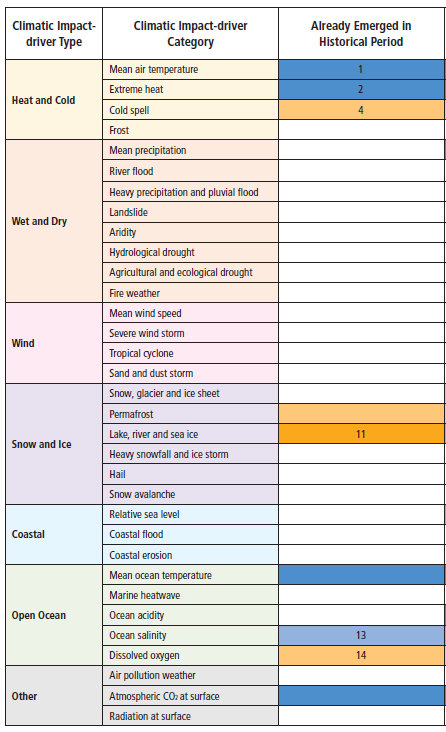
\includegraphics[width=0.7\textwidth]{bilder/bilderKlima-0076.png}\\[1cm]
\end{center}
\caption{Reproduktion von Spalte 1 von Tabelle 12.12, IPCC AR6 Working Group I-Bericht. Auftreten anthropogenen Signals in historischer Periode für CIDs gezeigt. Weiß: kein Signal detektiert. Blau und orange: Veränderung detektiert (Abnahme oder Zunahme) und Konfidenzniveau wie in Farblegende angegeben. Zahlen beziehen sich auf spezifische Regionen und Konfidenzniveaus: siehe originale Tabelle für Anmerkungen.}
\end{table}

\section{Attributions extremer Ereignisse (EEA)}
Bei der Untersuchung der IPCC-Behandlung der Attribution extremer Wetter- und Klimaereignisse im weiteren Sinne bietet AR6 eine zweideutige Bewertung der Rolle der anthropogenen Erwärmung, die zwischen den Kapiteln unterschiedlich ausfällt. Kapitel 11 von WG1 stellt fest (Seneviratne et al., 2021):

\begin{quote}
Die Belege für beobachtete Veränderungen bei Extremereignissen und ihre Attribution auf menschlichen Einfluss (einschließlich Treibhausgas- und Aerosolemissionen und Landnutzungsänderungen) haben sich seit AR5 verstärkt, insbesondere für extreme Niederschläge, Dürren, tropische Wirbelstürme und zusammengesetzte Extreme (einschließlich trocken/heißer Ereignisse und Feuerwetter). Einige jüngste heiße Extremereignisse wären ohne menschlichen Einfluss auf das Klimasystem extrem unwahrscheinlich aufgetreten.
\end{quote}

Im Gegensatz dazu zeichnet, wie in Abschnitt 8.5 erwähnt, Kapitel 12 von WG1 (Tabelle 12.12) ein anderes Bild – vermutlich kamen die Expertenbewertungen verschiedener Autorengruppen für die beiden Kapitel zu unterschiedlichen Schlussfolgerungen (Ranasinghe, 2021):

\begin{itemize}
\item Hohe Zuversicht in eine Zunahme extremer Hitzeereignisse in tropischen Regionen, wo Beobachtungen Trendschätzungen ermöglichen, und in den meisten Regionen der mittleren Breiten, mittlere Zuversicht anderswo 
\item Mittlere Zuversicht in eine Abnahme extremer Kälteereignisse in Australien, Afrika und dem größten Teil des nördlichen Südamerikas, wo Beobachtungen Trendschätzungen ermöglichen 
\item Keine Belege für das Auftreten in der historischen Periode einer Veränderung bei Flusshochwassern, starken Niederschlägen, Dürre, Feuerwetter, schweren Windstürmen und tropischen Wirbelstürmen 
\end{itemize}

Während die Gesamtfrage der Erkennung von Veränderungen bei Extremwetterereignissen und ihrer Attribution zweideutig bleibt, bezieht sich der Großteil der Aktivität in diesem Bereich auf die Attribution spezifischer Extremwetterereignisse.
Die prominenteste Anstrengung ist World Weather Attribution (WWA; worldweatherattribution.org), eine internationale Forschungsinitiative für die Attribution extremer Ereignisse, die vorgibt zu analysieren, wie der Klimawandel die Wahrscheinlichkeit und Intensität extremer Wetterereignisse beeinflusst. Ihr Ansatz besteht darin, große Ensembles regionaler Klimamodelle zu verwenden, um ein Ereignis im heutigen Klima mit einem in einem kontrafaktischen vorindustriellen Klima ohne menschliche Einflüsse zu vergleichen.

WWA hat eine prominente öffentliche Präsenz bei der Verknüpfung extremen Wetters mit dem Klimawandel, wobei ihre Pressemitteilungen beträchtliche Aufmerksamkeit in öffentlichen und politischen Diskussionen erregen. Jedoch haben WWAs umfassende Förderung nicht-peer-reviewter Befunde, ihr offenes Eingeständnis, Analysen zu gestalten, um Rechtsstreitigkeiten zu dienen, und ihre methodologischen Herausforderungen Kontroversen ausgelöst, wobei Kritiker die Robustheit und Unparteilichkeit ihrer Schlussfolgerungen in Frage stellen (Pielke Jr. 2024). Trotz dieser Probleme beeinflusst WWAs Arbeit weiterhin Klimawissenschafts- und Mediennarrative. Technische Kritiken des Ansatzes umfassen einen Mangel an einem formalen Erkennungsprozess; eine implizite Annahme, dass 100 Prozent der nachindustriellen Erwärmung durch Treibhausgase verursacht wird; und ein Versagen, interne Klimavariabilität angemessen zu berücksichtigen.

Da EEA relativ neu ist, sind viele grundlegende methodologische Fragen in der Expertenliteratur noch nicht geklärt. Eine wichtige Herausforderung ist der Mangel an Daten. Extreme Ereignisse sind per Definition selten. Viele Analysen extremer Ereignistypen (einschließlich der US National Assessment Reports) bewerten nur Daten seit 1950 oder 1970. Jedoch, wie in Kapitel 6 betont, traten viele der schlimmsten extremen Wetter- und Klimaereignisse in der US-Geschichte in oder vor der ersten Hälfte des 20. Jahrhunderts auf, einschließlich im frühen 19. Jahrhundert. Und wenn paläoklimatische Rekonstruktionen berücksichtigt werden, wird es sehr schwierig für ein Ereignis, Schwellenwerte dessen zu überschreiten, was von der natürlichen Variabilität erwartet wird, besonders wenn ein angemessen großes geografisches Gebiet betrachtet wird.

Eine weitere Herausforderung ist die Definition des zu untersuchenden Ereignisses. Es gibt eine langjährige Literatur in Statistik und Ökonometrie über die Herausforderung, Daten mit Ausreißern zu analysieren. Das Problem entsteht, weil eine Datenreihe eine Wahrscheinlichkeitsverteilung etabliert, die den erwarteten Bereich von Beobachtungen definiert. Wenn ein Ausreißer beobachtet wird, könnte dies anzeigen, dass sich der zugrundeliegende Prozess, der zur Datenverteilung führt, geändert hat (was im Wetterkontext bedeuten würde, dass ein Klimawandel erkannt wurde) oder dass der zugrundeliegende Prozess mehrere Regime mit jeweils unterschiedlicher Wahrscheinlichkeitsverteilung hat, wobei die Beobachtung eines Ausreißers einfach bedeutet, dass wir uns vorübergehend in einem anderen Regime befanden, aber das System selbst unverändert war. Wenn eine Zeitreihe nur ein einziges Ausreißerereignis am Ende der Reihe enthält, ist es nicht möglich zu bestimmen, welches Modell das richtige ist (Chen und Liu 1993). Zum Beispiel könnte es ein "gewöhnliches" Wetterregime geben, das eine Verteilung von Sommer-Tageshöchstwerten in einer bestimmten Küstenregion erzeugt, und ein zweites "Hitzewellen"-Regime, das eintritt, wenn ein Inland-Blockierungsereignis auftritt, was eine Temperaturverteilung erzeugt, die 15°C höher zentriert ist als die erste. Ein Tag mit Temperaturen 13°C über dem Normalwert wäre entweder eine extreme Hitze-Anomalie unter dem ersten Regime oder ein etwas kühles Ereignis unter dem zweiten, und wir haben in diesem Fall keine Möglichkeit, auf statistischen Grundlagen zu wissen, welche Sichtweise richtig ist.

Visser und Petersen (2012) und Sardeshmukh et al. (2015) weisen beide darauf hin, dass verschiedene Verteilungen beobachtete Daten gleich gut anpassen könnten, aber sehr unterschiedliche Implikationen über die Wahrscheinlichkeit eines spezifischen Wetterereignisses ergeben. Visser und Petersen argumentieren, dass angesichts der tiefen Ungewissheiten der Extremwetter-Analyse eine Verbindung zwischen individuellen Ereignissen und globalem Klimawandel vermieden werden sollte. Außerdem wirft die Existenz eines Ausreißers am Ende einer Datenreihe das Problem auf, dass Schätzungen der Ereigniswahrscheinlichkeiten verzerrt sein werden, ob der Ausreißer eingeschlossen oder ausgeschlossen wird (Barlow et al., 2020). Methoden zur Beseitigung der Verzerrung sind noch nicht etabliert, was einige Experten (z.B. Miralles und Davison 2023) dazu führt zu argumentieren, dass in Situationen, in denen eine Datenreihe ein einzelnes extremes Ereignis am Ende enthält, die Schätzung einer Wiederkehrperiode für das extreme Ereignis so verzerrt und ungewiss sein wird, dass sie ganz vermieden werden sollte.

Wir stellen eine Fallstudie eines jüngsten extremen Ereignisses mit hoher Auswirkung in den USA bereit, um die Herausforderungen und Zweideutigkeiten bei der Attribution der Häufigkeit und Intensität extremer Wetterereignisse auf menschlich verursachte Erwärmung zu illustrieren.

\subsection{Fallstudie – 2021 Western North America Hitzewelle}
Die 2021 Western North America Hitzewelle war ein extremes Ereignis, das viel von Western North America Ende Juni 2021 betraf. Oberflächentemperaturrekorde wurden in Portland, OR (\SI{116}{F}; vorheriger Rekord 107°F) und Seattle, WA (\SI{108}{F}; vorheriger Rekord \SI{103}{F}) aufgestellt (Mass et al., 2024).

Das WWA-Team erzeugte internationale Schlagzeilen mit ihrer Analyse, die die folgenden Attributionsaussagen bereitstellte (WWA, 2021; Philip et al., 2022):

\begin{itemize}
\item Basierend auf Beobachtungen und Modellierung war das Auftreten dieser Hitzewelle praktisch unmöglich ohne menschlich verursachten Klimawandel. 
\item Das Ereignis wird als etwa ein 1-in-1000-Jahre-Ereignis im heutigen Klima geschätzt. 
\item Das Ereignis wäre mindestens 150-mal seltener ohne menschlich induzierten Klimawandel gewesen. 
\item Diese Hitzewelle war etwa \SI{2}{\celsius} heißer als sie gewesen wäre, wenn sie zu Beginn der industriellen Revolution aufgetreten wäre (als die globalen Durchschnittstemperaturen \SI{1.2}{\celsius} kühler waren als heute). 
\end{itemize}

Aber ein wichtiger Einwand gegen die erste Behauptung ist, dass andere Forscher aus historischen Wetterdaten schlossen, dass während eine Hitzewelle der beobachteten Magnitude tatsächlich praktisch unmöglich ohne anthropogenen Klimawandel war, sie auch praktisch unmöglich mit Klimawandel war. Bercos-Hickey (2022) bemerkte \emph{diese Temperaturen waren praktisch unmöglich unter allen zuvor erfahrenen meteorologischen Bedingungen, mit oder ohne globale Erwärmung.} McKinnon und Simpson (2022) erklärten "die wahrscheinlichste Erklärung bleibt, dass das Wetterereignis selbst \emph{'Pech'} war." Das 2023 Oregon Climate Assessment (Fleischman, 2023) schloss, dass sich die Hitzekuppel auch ohne Klimawandel gebildet hätte und \emph{Es gibt keine Belege dafür, dass die höchst ungewöhnliche Kombination von Wettermerkmalen, die die Hitzekuppel antrieben, durch den Klimawandel wahrscheinlicher gemacht wurden, und Klimamodelle projizieren keine Zunahme der Häufigkeit von Hochdruckrücken über dem Pacific Northwest} (Fleischman, 2023, S. 49).

Mass et al. (2024) fasst die unmittelbare Abfolge zusammengesetzter Ereignisse zusammen, die zur Hitzewelle führten. Es gab einen rekordverdächtigen mitteltroposphärischen Rücken über dem Pacific Northwest, erzwungen durch eine tropische Störung im westlichen Pazifik. Dies produzierte rekordverdächtige mitteltroposphärische Temperaturen, starke Subsidenz in der unteren Atmosphäre, Ostwind auf niedrigem Niveau, der Hangabwärts-Erwärmung auf regionalem Gelände produzierte und die Entfernung kühlerer Meeresluft, und ein sich nähernder Trog auf niedrigem Niveau, der den Hangabwärts-Fluss verstärkte. Das Ereignis trat zu einer Zeit maximaler solarer Einstrahlung und trockenerer als normale Bodenfeuchtigkeit auf. Mit einem Storyline-Ansatz bewerteten Mass et al., dass es keinen Trend in Dürre und trockenen Böden im Pacific Northwest gab; es gibt keine Belege dafür, dass die globale Erwärmung stärkere Hochdruckrücken produziert, und keinen beobachteten Trend in Hitzewellen oder Rekordtemperaturen in der Region. Sie schlossen, dass obwohl anthropogene Erwärmung bis zu \SI{2}{F} zur Magnitude des Ereignisses beigetragen haben könnte, es wenige Belege für weitere Verstärkung des Ereignisses durch zunehmende Treibhausgase gibt.

Bercos-Hickey et al. (2022) führten eine statistische Analyse einer modellbasierten Attributionsstudie dieser Hitzewelle durch. Da das Ereignis ein weit entfernter Ausreißer und weit über den Grenzen von Generalisierten Extremwert-Verteilungen ist, die aus historischen Daten angepasst wurden, schlossen sie, dass Schätzungen von Wiederkehrzeiten, quantitative Veränderungen in Ereignismagnitude und -häufigkeit und Wahrscheinlichkeit der extremen Temperaturen wie von der WWA bereitgestellt nicht akkurat sind und als niedrige Zuversicht interpretiert werden sollten. Sie fanden, dass Hindcast-Attributionsmethoden unter Verwendung eines Ensembles regionaler Klimamodelle, kombiniert mit Pearl (2009) kausalen Schlussfolgerungen, begrenzte und bedingte Informationen über die Magnitude des menschlichen Einflusses auf diese Hitzewelle liefern können - sie lieferten eine stärker eingeschränkte Schätzung, dass menschliche Aktivitäten einen $\approx$\SI{1.4}{F} - \SI{1.8}{F} Anstieg der täglichen Maximaltemperaturen verursachten.

Zeder et al. (2023) schlossen ebenfalls, dass die von Philip et al. (2022, die WWA-Analyse) verwendeten Methoden dazu neigen, die Seltenheit extremer Hitzewellen zu übertreiben, was zu einer verzerrten Wahrnehmung der Auswirkung des Klimawandels auf das Hitzewellenereignis führt: \emph{Die Tendenz, die Wiederkehrperiode beobachteter extremer Hitzewellenereignisse zu überschätzen, kann den Eindruck nähren, dass scheinbar unmögliche Hitzewellen-Extreme derzeit mit einer beispiellosen Rate clustern.}

Die 2021 Western North America Hitzewelle war ein seltenes und beispielloses zusammengesetztes Wetterereignis, das jahrhundertealte Temperaturrekorde um bis zu \SI{9}{F} brach. Während das WWA-Team weltweite Publizität für ihre schnellen Attributionsbehauptungen erhielt, die den anthropogenen Klimawandel beschuldigten, zeigten nachfolgende peer-reviewte Analysen, dass das Ereignis durch seltene meteorologische Bedingungen verursacht wurde, die nicht durch die globale Erwärmung wahrscheinlicher gemacht wurden.

\vfill
\noindent\textbf{Literaturverzeichnis:}

\begingroup
\parindent=0pt
\everypar{\hangindent=2em\hangafter=1\relax}
Allen, M. R., \& Tett, S. F. B. (1999). Checking for model consistency in optimal fingerprinting. Climate
Dynamics, 15(6), 419–434. https://doi.org/10.1007/s003820050291

AR4: Intergovernmental Panel on Climate Change Fourth Assessment Report (2021) Working Group I
Contribution. www.ipcc.ch.

AR5: Intergovernmental Panel on Climate Change Fifth Assessment Report (2021) Working Group I
Contribution. www.ipcc.ch.

AR6: Intergovernmental Panel on Climate Change Sixth Assessment Report (2021) Working Group I
Contribution. www.ipcc.ch.

Arthun, M, RCJ Willis, HL Johnson, L Chafik, HR Langehaug (2021) Mechanisms of Decadal North
Atlantic Climate Variability and Implications for the Recent Cold Anomaly. Journal of Climate, Vol 34

Balcombe, Kevin, Iain Fraser and Abhijit Sharma (2019) Is radiative forcing cointegrated with temperature?
A further examination using a structural time series approach.” Management of Environmental Quality
30(5) DOI 10.1108/MEQ-12-2018-021.

Barlow, Anna Maria, Chris Sherlock and Jonathan Tawn (2020) Inference for Extreme Values Under
Threshold-Based Stopping Rules. Journal of the Royal Statistical Society Series C August 2020,
Pages 765–789, https://doi.org/10.1111/rssc.12420

Bednarz, EW, AH Butler, X Wang, Z Zhou, W Yu, G Stenchikov, M Toohey, Y Zhu (2025) Indirect
climate impacts of the Hunga eruption. Preprint, https://doi.org/10.5194/egusphere-2025-1970

Bercos-Hickey, E., et al. (2022). Anthropogenic contributions to the 2021 Pacific Northwest heatwave.
Geophysical Research Letters, 49(23), e2022GL099396. \url{https://doi.org/10.1029/2022GL099396
}
Bokuchava, DD and VV Semenov (2021) Mechanisms of the early 20th century warming in the Arctic.
Earth-Science Reviews, 222, 103820

Chatzistergos, T., Krivova, N. A., \& Yeo, K. L. (2023). Long-term changes in solar activity and
irradiance. Journal of Atmospheric and Solar-Terrestrial Physics, 252, 106150.
https://doi.org/10.1016/j.jastp.2023.106150

Chen, C., \& Liu, L.-M. (1993). Joint estimation of model parameters and outlier effects in time series.
Journal of the American Statistical Association, 88(421), 284–297.
http://www.jstor.org/stable/2290724

Chen, H, SX Chen and M Mu (2023) A statistical review on the optimal fingerprinting approach in climate
change studies. Climate Dynamics 62:1439-1446 \url{https://link.springer.com/article/10.1007/s00382-
023-06975-5}

Chylek, P., et al. (2016). The role of Atlantic Multi-Decadal Oscillation in the global mean temperature
variability. Climate Dynamics, 47(9–10), 3271–3279. https://doi.org/10.1007/s00382-016-3025-7

Connolly, R., et al. (2021). How much has the sun influenced Northern Hemisphere temperature trends?
An ongoing debate. Research in Astronomy and Astrophysics, 21(6), 131.
https://doi.org/10.1088/1674-4527/21/6/131

Cramer, W., et al. (2014). Detection and attribution of observed impacts. In C. B. Field et al. (Eds.),
Climate Change 2014: Impacts, Adaptation, and Vulnerability. Part A: Global and Sectoral Aspects
(pp. 979–1037). Cambridge University Press.

Dagsvik, JK SH Moen (2023) To what extent are temperature levels changing due to greenhouse gas
emissions? Statistics Norway Discussion Paper 1007 September 2023

Dagsvik, JK, M Fortuna and SH Moen (2020) How Does Temperature Vary Over Time?: Evidence on the
Stationary and Fractal Nature of Temperature Fluctuations. Journal of the Royal Statistical Society
Series A: Statistics in Society, Volume 183, Issue 3, June 2020, Pages 883–908,
https://doi.org/10.1111/rssa.12557

Davidson, James E.H., David B. Stephenson and Alemtsehai A. Turasie (2015) Time series modeling of
paleoclimate data Environmetrics 27(1) \url{https://onlinelibrary.wiley.com/doi/abs/10.1002/env.2373}

Dergiades, T., R.K. Kaufmann and T. Panagiotidis (2016). Long-run changes in radiative forcing and
surface temperature: The effect of human activity over the last five centuries. Journal of Environmental
Economics and Management 76:67—85.
https://www.sciencedirect.com/science/article/abs/pii/S0095069615000911

England, Mark, Lorenzo M Polvani, James A Screen, et al (2025). Surprising, but not unexpected, multi-
decadal pause in Arctic sea ice loss. ESS Open Archive. March 29, 2025.

Fleishman, E., editor. (2023). Sixth Oregon Climate Assessment. Oregon Climate Change Research
Institute, Oregon State University, Corvallis, Oregon. \url{https://blogs.oregonstate.edu/occri/oregon-climate-assessments}

Forster et al. (2024) “Indicators of Global Climate Change 2024: annual update of key indicators of the
state of the climate system and human influence” Earth System Science Data 17(6)
https://doi.org/10.5194/essd-17-2641-2025

Frajka-Williams, E, C Beaulieu, Aurelie Duchez (2017) Emerging negative Atlantic Multidecadal
Oscillation index in spite of warm subtropics. Scientific Reports, 7:11224

Goessling, Helge F. Thomas Rackow and Thomas Jung (2024) Recent global temperature surge
intensified by record-low planetary albedo. Science Vol 387, Issue 6729 pp. 68-73
https://www.science.org/doi/abs/10.1126/science.adq7280

Gulev, S. K., et al. (2021). Changing state of the climate system. In V. Masson-Delmotte et al. (Eds.),
Climate Change 2021: The Physical Science Basis. Contribution of Working Group I to the Sixth
Assessment Report of the Intergovernmental Panel on Climate Change (pp. 287–422). Geneva:
Intergovernmental Panel on Climate Change.

Hansen J and P Karecha (2025) Large cloud feedback confirms high sensitivity.
\url{https://www.columbia.edu/~jeh1/mailings/2025/CloudFeedback.13May2025.pdf}

Hegerl, G. C., et al. (2007). Understanding and attributing climate change. In S. Solomon et al. (Eds.),
Climate Change 2007: The Physical Science Basis. Contribution of Working Group I to the Fourth
Assessment Report of the Intergovernmental Panel on Climate Change (pp. 663–745). Cambridge
University Press.

Hegerl, GC, S Bronniman, A Schurer et al. (2017) Early 20th century warming: Anomalies, causes and
consequences. WIRES Climate Change, DOI: 10.1002/wcc.522

Hegerl, GC, S Bronniman, T Cowan (2019) Causes of climate change over the historical record.
Environmental Research Letters, 14, 123006

Hodnebrog, Ø et al. (2024), Recent reductions in aerosol emissions have increased Earth’s energy
imbalance. Communications Earth and Environment 5, 166 (2024). doi:10.1038/s43247-024-01324-8

Houghton, J. T., et al. (Eds.). (2001). Climate Change 2001: The Scientific Basis. Contribution of
Working Group I to the Third Assessment Report of the Intergovernmental Panel on Climate Change
(pp. 1–881). Cambridge University Press.
https://mailchi.mp/caa/large-cloud-feedback-confirms-high-climate-sensitivity

Kravtsov, S., Westgate, A., \& Gavrilov, A. (2024). Global-scale multidecadal variability in climate
models and observations, part II: The stadium wave. Climate Dynamics, 62, 10281–10306.
https://doi.org/10.1007/s00382-024-07451-4

Kuchar, A., Sukhodolov, T., Chiodo, G., Jörimann, A., Kult-Herdin, J., Rozanov, E., and Rieder, H. H.
(2025): Modulation of the northern polar vortex by the Hunga Tonga–Hunga Ha'apai eruption and the
associated surface response, Atmospheric Chemistry and Physics, 25, 3623–3634,
https://doi.org/10.5194/acp-25-3623-2025.

Lewis, Nicholas (2023) “Objectively Combining Climate Sensitivity Evidence,” Climate Dynamics 61,
no. 9–10 (2023): 3155–3163, https://doi.org/10.1007/s00382-022-06398-8 .

Lockwood, M. (2012). Solar influence on global and regional climates. Surveys in Geophysics, 33(3–4),
503–534. https://doi.org/10.1007/s10712-012-9181-3

Loeb, N. G. et al. (2019) Decomposing Shortwave Top-of-Atmosphere and Surface Radiative Flux
Variations in Terms of Surface and Atmospheric Contributions. Journal of Climate 32(16), 5003-
5019 (2019). doi:10.1175/JCLI-D-18-0826.1

Loeb, N., S-H Ham, RP Allen, TJ Thorsen, B Meyssignac, S Kato, GC Johnson, JL Lyman (2024)
Observational Assessment of Changes in Earth’s Energy Budget since 2000. Surveys in Geophysics,
45, 1757-1783

Mass, C., et al. (2024). The Pacific Northwest heat wave of 25–30 June 2021: Synoptic/mesoscale
conditions and climate perspective. Weather and Forecasting, 39(2), 275–291.
https://doi.org/10.1175/WAF-D-23-0154.1

Matthes, K., et al. (2017). Solar forcing for CMIP6 (v3.2). Geoscientific Model Development, 10(6),
2247–2302. https://doi.org/10.5194/gmd-10-2247-2017

McKinnon, K. and I. Simpson (2022) How Unexpected Was the 2021 Pacific Northwest Heatwave?
Geophysical Research Letters, 49, e2022GL100380. \url{https://doi.org/10.1029/2022GL100380}

McKinnon, K. and I. Simpson (2022) How Unexpected Was the 2021 Pacific Northwest Heatwave?
Geophysical Research Letters, 49, e2022GL100380. \url{https://doi.org/10.1029/2022GL100380}

McKitrick, R. (2021). Checking for model consistency in optimal fingerprinting: A comment. Climate
Dynamics, 58(1–2), 405–411. https://doi.org/10.1007/s00382-021-05913-7

McKitrick, R. (2023). Total least squares bias in climate fingerprinting regressions with heterogeneous
noise variances and correlated explanatory variables. Environmetrics, 35(2), e2835.
https://doi.org/10.1002/env.2835

McKitrick, Ross R (2022) On the choice of TLS versus OLS in climate signal detection
regression. Climate Dynamics 10.1007/s00382-022-06315-z

McKitrick, Ross R (2025) Consistent Climate Fingerprinting. Climate Dynamics forthcoming preprint
available at www.rossmckitrick.com

McLean, J.D., C. R. de Freitas, and R. M. Carter, (2009) “Influence of the Southern Oscillation on
Tropospheric Temperature,” Journal of Geophysical Research: Atmospheres 114, no. D14 (July 23,
2009): D14104, https://doi.org/10.1029/2008JD011637.

Miralles, Ophélia and Anthony Davison (2023) Timing and spatial selection bias in rapid extreme event
attribution. Weather and Climate Extremes 41 100584 \url{https://doi.org/10.1016/j.wace.2023.100584}

Myhre, G., D. Shindell, F.-M. Bréon, et al (2013): Anthropogenic and Natural Radiative Forcing. In:
Climate Change 2013: The Physical Science Basis. Contribution of Working Group I to the Fifth
Assessment Report of the Intergovernmental Panel on Climate Change [Stocker, T.F., et al. (eds.)].
Cambridge University Press, Cambridge, United Kingdom and New York, NY, USA.

Nissan, Hannah, Lisa Goddard, Erin Coughlan de Perez, et al. (2019) On the use and misuse of climate
change projections in international development. Wires Climate Change 14 March 2019
https://doi.org/10.1002/wcc.579

Palmer, Tim N and Bjorn Stevens (2019) The scientific challenge of understanding and estimating
climate change. Proceedings of the National Academy of Sciences 116 (49) 24390-24395
https://doi.org/10.1073/pnas.1906691116

Pearl, J. (2009). Causality. Cambridge University Press.

Philip, S. Y., et al. (2022). Rapid attribution analysis of the extraordinary heatwave on the Pacific coast of
the U.S. and Canada June 2021. Earth System Dynamics, 13(4), 1689–1713.
https://doi.org/10.5194/esd-13-1689-2022

Pielke Jr., Roger (2024) Weather Attribution Alchemy. Substack essay
\url{https://rogerpielkejr.substack.com/p/weather-attribution-alchemy}

Ranasinghe, R., Ruane, A. C., Vautard, R., Arnell, N., Coppola, E., Cruz, F. A., ... Zaaboul, R. (2021).
Chapter 12: Climate change information for regional impact and for risk assessment. In V. Masson-
Delmotte et al. (Eds.), Climate Change 2021: The Physical Science Basis. Contribution of Working
Group I to the Sixth Assessment Report of the Intergovernmental Panel on Climate Change (pp.
1767–1926). Cambridge University Press. https://doi.org/10.1017/9781009157896.014

Razzak, Weshah A. (2022). "The Econometrics of Global Warming," Journal of Economics and
Econometrics, vol. 65(2), pages 13-47.

Sardeshmukh, P. D., Compo, G. P., \& Penland, C. (2015). Need for caution in interpreting extreme
weather statistics. Journal of Climate, 28(23), 9166–9187. https://doi.org/10.1175/JCLI-D-15-0020.1

Scafetta, N. (2013). Discussion on climate oscillations: CMIP5 general circulation models versus a semi-
empirical harmonic model based on astronomical cycles. Earth-Science Reviews, 126, 321

Scaffeta, Nicola (2021) “Reconstruction of the Interannual to Millennial Scale Patterns of the Global
Surface Temperature,” Atmosphere 12, no. 2: 147, \url{https://doi.org/10.3390/atmos12020147}

Schmidt, G. (2024) Climate models can’t explain 2023’s huge heat anomaly — we could be in uncharted
territory. Nature 627, 467. https://www.nature.com/articles/d41586-024-00816-z

Schmutz, Werner K. (2021) “Changes in the Total Solar Irradiance and Climatic Effects,” Journal of
Space Weather and Space Climate 11: 40, https://doi.org/10.1051/swsc/2021016.

Seneviratne, S. et al. (2021) “Chapter 11: Weather and Climate Extreme Events in a Changing Climate.”
In Climate Change 2021: The Physical Science Basis. Contribution of Working Group I to the Sixth
Assessment Report of the Intergovernmental Panel on Climate Change, edited by V. Masson-
Delmotte, P. Zhai, A. Pirani, S.L. Connors, C. Péan, S. Berger, N. Caud, et al., 1513–1766.
Cambridge: Cambridge University Press, 2021. https://doi.org/10.1017/9781009157896.013.

Solanki, S.K. et al. (2004), “Unusual Activity of the Sun during Recent Decades Compared to the
Previous 11,000 Years,” Nature 431, no. 7012 (October 28, 2004): 1084–1087,
https://doi.org/10.1038/nature02995.

Stefani, Frank (2021) “Solar and Anthropogenic Influences on Climate: Regression Analysis and
Tentative Predictions,” Climate 9, no. 11 (November 3, 2021): 163,
https://doi.org/10.3390/cli9110163.

Thompson, DJW, JM Wallace, JJ Kennedy, PD Jones (2010) An abrupt drop in Northern Hemisphere Sea
Surface Temperature around 1970. Nature, 467, 444-447

Tokinaga, H, SP Xie, and H Mukougawa (2017) Early 20th century Arctic warming intensified by
Pacific and Atlantic multidecadal variability. Proceedings of the National Academy of Sciences, 114,
6227-6233 https://www.pnas.org/doi/abs/10.1073/pnas.1615880114

Tung, Ka-Kit and Jiansong Zhou (2013) “Using Data to Attribute Episodes of Warming and Cooling in
Instrumental Records,” Proceedings of the National Academy of Sciences 110, no. 6 (January 23,
2013): 2058–2063, https://doi.org/10.1073/pnas.1212471110.

Usoskin, I.G., S. K. Solanki, and G. A. Kovaltsov (2007) “Grand Minima and Maxima of Solar Activity:
New Observational Constraints,” Astronomy \& Astrophysics 471, no. 1 (June 6, 2007): 301–309,
https://doi.org/10.1051/0004-6361:20077704.

Velasco Herrera, V.M., B. Mendoza, and G. Velasco Herrera (2015) “Reconstruction and Prediction of
the Total Solar Irradiance: From the Medieval Warm Period to the 21st Century,” New Astronomy 34
(January 2015): 221–233, https://doi.org/10.1016/j.newast.2014.07.009.

Visser, H. and A.C. Petersen (2012) Inferences on weather extremes and weather-related disasters: a
review of statistical methods Climates of the Past 8, 265–286
\url{https://cp.copernicus.org/articles/8/265/2012/cp-8-265-2012.pdf}

World Weather Attribution (2021) “Western North American Extreme Heat Virtually Impossible without
Human-Caused Climate Change.” July 7, 2021. \url{https://www.worldweatherattribution.org/western-
north-american-extreme-heat-virtually-impossible-without-human-caused-climate-change/.}

Yuan, et al. (2024) Abrupt reduction in shipping emission as an inadvertent geoengineering termination
shock produces substantial radiative warming. Communications Earth and Environment 5, 281
(2024). doi:10.1038/s43247-024-01442-3

Zeder, J., Sippel, S., Pasche, O. C., Engelke, S., \& Fischer, E. M. (2023). The effect of a short
observational record on the statistics of temperature extremes. Geophysical Research Letters, 50,
e2023GL104090. https://doi.org/10.1029/2023GL104090
\endgroup


\cleardoublepage
\chapter*{TEIL III: AUSWIRKUNGEN AUF ÖKOSYSTEME UND GESELLSCHAFT}
\FigureNumbersByChapter
\addcontentsline{toc}{chapter}{TEIL III: AUSWIRKUNGEN AUF ÖKOSYSTEME UND GESELLSCHAFT}
\cleardoublepage
%\numberwithin{figure}{chapter}
\chapter{KLIMAWANDEL UND US-LANDWIRTSCHAFT}
\paragraph{Kapitelzusammenfassung}
\begin{quote}
Es gibt reichliche Belege, die Jahrzehnte zurückreichen, dass steigende CO$_2$-Konzentrationen Pflanzen, einschließlich landwirtschaftlicher Nutzpflanzen, zugutekommen, und dass die CO$_2$-induzierte Erwärmung ein Nettonutzen für die US-Landwirtschaft sein wird. Die Zunahme des atmosphärischen CO$_2$ hat auch die Produktivität aller wichtigen US-Nutzpflanzenarten gesteigert. Es gibt Grund zu dem Schluss, dass der Klimawandel insgesamt für die meiste US-Landwirtschaft neutral oder vorteilhaft war und weiterhin sein wird.
\end{quote}
\section{Ökonometrische Analysen}
Ökonometrische Analysen der Auswirkungen des Klimawandels auf die Landwirtschaft haben versucht, Informationen über langfristige Veränderungen der Nutzpflanzenerträge als Reaktion auf Temperatur- und Niederschlagsveränderungen unter Annahmen über adaptives Verhalten der Landwirte zu integrieren. Eine Methode konzentriert sich auf Variationen in landwirtschaftlichen Grundstückswerten. Die Begründung ist, dass wenn Klimawandel ein langfristiger Nettonutzen für die Landwirtschaft ist, er sich in höheren Marktwerten für landwirtschaftliche Flächen niederschlagen sollte, und umgekehrt. Während einzelne Nutzpflanzen vom Klimawandel profitieren oder geschädigt werden könnten, stellt der Wert von Ackerland, sobald die adaptiven Reaktionen der Landwirte berücksichtigt werden, einen Index dar, ob die Veränderungen voraussichtlich vorteilhaft sind oder nicht.
Mendelsohn et al. (1994) untersuchten die Beziehung zwischen historischen klimatischen Variationen und landwirtschaftlichen Grundstückswerten und kamen zu dem Schluss, dass die globale Erwärmung der amerikanischen Landwirtschaft leicht zugutekommen würde.

Die Methode von Mendelsohn et al., Ricardo-Analyse genannt nach David Ricardo, dem britischen Ökonomen des 19. Jahrhunderts, der die Untersuchung von Grundstückswerten pionierte, zog anschließend Kritik von Autoren auf sich, die argumentierten, sie habe es versäumt, Unterschiede in Grundstückswerten zu berücksichtigen, die auf feste standortbezogene Eigenschaften wie Bodenqualität und nicht-klimatische Veränderungen einschließlich nahegelegener Urbanisierung zurückzuführen sind. Deschênes und Greenstone (2007) betrachteten landwirtschaftliche Gewinne anstatt Grundstückswerte und erreichten ähnliche Schlussfolgerungen wie Mendelsohn et al. (1994), nämlich dass vergangene klimatische Variationen relativ wenig Auswirkung auf die Rentabilität von Betrieben hatten und dass Erwärmung wahrscheinlich kleine Gesamtvorteile für den US-Landwirtschaftssektor erbringen würde. Jedoch führte ein nachfolgender Austausch mit Kritikern dazu, dass sie (Deschênes und Greenstone 2012) ihre Schlussfolgerungen revidierten und potenziell große Verluste in der US-Landwirtschaft aufgrund der Klimaerwärmung projizierten.

Burke und Emerick (2016) betrachteten Temperaturvariationen über 1980 bis 2000 und argumentierten, dass Landwirte nicht so fähig waren, sich an Temperaturveränderungen anzupassen, wie die Ricardo-Methode annimmt, und dass Klimawandel große negative Auswirkungen auf Mais- und Sojabohnenerträge haben würde. Schlenker und Roberts (2009) argumentierten ähnlich, dass Ertragsgewinne durch vergangene Erwärmung sich nicht in die Zukunft übertragen würden und Mais- und Sojabohnenerträge dieses Jahrhundert aufgrund des Klimawandels stark abnehmen würden.

Zwei kürzlich durchgeführte Studien haben argumentiert, dass pessimistische Befunde wie diese nicht robust sind. Ortiz-Bobea (2019) argumentierte, dass Grundstückswerte landwirtschaftliche und nicht-landwirtschaftliche Einflüsse aggregieren und letztere herausgefiltert werden müssen. Er entwickelte einen Datensatz unter Verwendung von Barpachten für landwirtschaftliche Aktivitäten als Maß für den Grundstückswert spezifisch für landwirtschaftliche Tätigkeit. Während das Grundstückswertmodell zukünftige Verluste unter Klimaerwärmung implizierte, tat dies das gleiche Modell unter Verwendung von Barpachten nicht, was den Autor zu dem Schluss führte, dass die pessimistischen Ergebnisse auf die Verwendung eines ungenauen Maßes für die Erträge aus landwirtschaftlicher Tätigkeit zurückzuführen waren. Bareille und Chakir (2023) stellten eine große Datenbank zu Betriebsverkaufspreisen in Frankreich für Grundstücke zusammen, die zwischen 1996 und 2019 zweimal verkauft wurden. Sie konnten pessimistische Ergebnisse replizieren, die negative Auswirkungen der Erwärmung auf landwirtschaftliche Grundstückswerte zeigten, unter Verwendung konventioneller ökonometrischer Modellierung. Aber indem sie die Wiederholungsverkaufsdaten nutzten, die Informationen über standortspezifische Veränderungen der Grundstückspreise lieferten, fanden sie, dass sich die Ergebnisse umkehrten und implizierten, dass Klimawandel sehr vorteilhaft für die französische Landwirtschaft sein wird. Die Autoren kamen zu dem Schluss, dass unter Berücksichtigung der Anpassung ein sich erwärmendes Klima positive Vorteile für die französische Landwirtschaft erbringen würde, die zwischen zwei- und 20-mal größer waren als zuvor geschätzt. Im Durchschnitt kamen sie mit vollständiger Anpassung zu dem Schluss, dass Klimaveränderungen unter dem mittleren RCP4.5-Szenario den Wert französischer Ackerflächen bis 2100 verdoppeln könnten.

Ein wesentlicher Mangel all dieser Studien ist jedoch, dass sie die Rolle der CO$_2$-Düngung auslassen. Klimawandel, wie er sich auf diesen Bericht bezieht, wird durch THG-Emissionen verursacht, hauptsächlich CO$_2$. Die oben zitierten ökonometrischen Analysen konzentrieren sich nur auf Temperatur- und Niederschlagsveränderungen und berücksichtigen nicht den vorteilhaften Wachstumseffekt des zusätzlichen CO$_2$, das sie antreibt. Wie in Kapitel 2 erklärt, ist CO$_2$ ein wichtiger Antrieb des Pflanzenwachstums, sodass diese Auslassung die Analyse hin zu einer Unterschätzung der Vorteile des Klimawandels für die Landwirtschaft verzerrt.

\section{Feld- und Laborstudien der CO$_2$-Anreicherung}
Eine der Methoden, mit der die Auswirkung von CO$_2$ auf das Nutzpflanzenwachstum untersucht wurde, sind "Freiluft-Anreicherungsexperimente" oder FACE-Plots, bei denen kleine CO$_2$-Quellen in Feldern um Pflanzen herum platziert werden und die Wachstumsreaktion auf erhöhtes CO$_2$ unter verschiedenen Wetterbedingungen aufgezeichnet wird. Ainsworth et al. (2020) fasst Ergebnisse von etwa 250 solcher Studien zusammen. Sie fanden heraus, dass eine Erhöhung des CO$_2$ um \SI{200}{ppm} eine durchschnittliche 18-prozentige Steigerung des Nutzpflanzenertrags bei C3-Pflanzen verursachte. C4-Pflanzen zeigten Vorteile hauptsächlich unter Dürrebedingungen.

Zusätzlich zu FACE-Plot-Experimenten gab es Tausende von Laborexperimenten über die Auswirkungen von CO$_2$ auf alle Arten von Pflanzenwachstum. Hier überprüfen wir einige der Ergebnisse zu wichtigen US-landwirtschaftlichen Nutzpflanzen.

\emph{Sojabohne}

Studien über die Auswirkung von erhöhtem CO$_2$ auf Sojabohnenpflanzen (Glycine max (L.) Merr.) in der wasserarmen Region der Huang-Huai-Hai-Ebene, China, zeigten, dass erhöhte CO$_2$-Konzentrationen die Photosyntheserate, Wassernutzungseffizienz und das Wachstum Li (2013) sowohl unter normalen Bedingungen als auch unter Dürrebedingungen verbesserten. Die Website CO2Science.org berichtet über 108 veröffentlichte Experimente zwischen 1985 und 2019, die Sojabohnen erhöhten CO$_2$-Konzentrationen aussetzten. Umgerechnet auf eine +\SI{300}{ppm}-Standardskala betrug der durchschnittliche Wachstumsvorteil +50,9 Prozent. Es gab auch zehn Studien, die über +\SI{600}{ppm} CO$_2$-Anreicherung berichteten, was die Photosynthese um durchschnittlich 90,3\% steigerte.

\emph{Mais (Corn)}

Die Website CO2Science.org berichtet über 28 veröffentlichte Experimente zwischen 1983 und 2018, die Mais (Zea mays L.) erhöhten CO$_2$-Konzentrationen aussetzten. Umgerechnet auf eine +\SI{300}{ppm}-Standardskala betrug der durchschnittliche Wachstumsvorteil +23,7 Prozent. Mais profitiert auch von erhöhter Dürretoleranz unter erhöhtem CO$_2$. Eine experimentelle Studie (Allen Jr., 2011) setzte Pflanzen Wasserstressbedingungen in sonnenbeschienenen kontrollierten Umgebungskammern bei \SI{360}{ppm} (Umgebungs-) und \SI{720}{ppm} (erhöhtem) CO$_2$ aus. Der Dürrestress verursachte einen 41-prozentigen Wachstumsverlust unter Umgebungs-CO$_2$, aber nur einen 13-prozentigen Verlust unter erhöhtem CO$_2$.

\emph{Weizen}

Die Website CO2Science.org berichtet über 92 veröffentlichte Experimente zwischen 1983 und 2020, die gewöhnlichen Weizen (Triticum aestivum L.) erhöhten CO$_2$-Konzentrationen aussetzten. Umgerechnet auf eine +\SI{300}{ppm}-Standardskala betrug der durchschnittliche Wachstumsvorteil +67,6 Prozent. Blandino (2020) maß sowohl den Ertrag als auch die Nährqualität einer "Improver"-Hybrid-Weizensorte und ihrer Eltern unter erhöhten CO$_2$-Konzentrationen (+\SI{166}{ppm}). Sie berichteten von einer Kornertragssteigerung von +16 Prozent, aber einem 7-prozentigen Rückgang der Kornproteingehalte. Aber sie fanden auch, dass die Lebensmittelqualität verschiedener Weizensorten unterschiedlich auf erhöhte CO$_2$-Konzentrationen reagierte, sodass bei ordnungsgemäßer Sortenauswahl Erzeuger Weizenarten auswählen könnten, die das erhöhte CO$_2$ am besten nutzen.

\begin{figure}[H]
\begin{center}
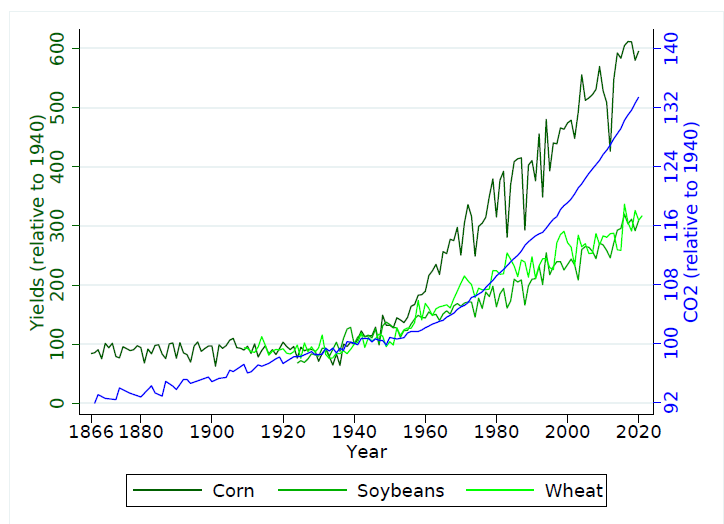
\includegraphics[width=0.9\textwidth]{bilder/bilderKlima-0078.png}\\[1cm]
\end{center}
\caption{Durchschnittliche CO$_2$-Werte und Erträge von Mais, Soja und Weizen in den USA, alle normalisiert
auf 1940=100. Quelle: Taylor und Schlenker (2021)}
\end{figure}

\emph{Weitere Belege}

Ein Bericht von 2021 des U.S. National Bureau of Economic Research (Taylor und Schlenker 2021) verwendete satellitengemessene Beobachtungen der CO$_2$-Konzentrationen im Freien in den Vereinigten Staaten, abgeglichen mit landkreisweisen landwirtschaftlichen Produktionsdaten und anderen wirtschaftlichen Variablen. Nach Kontrolle der Auswirkungen von Wetter, Umweltverschmutzung und Technologie kamen die Autoren zu dem Schluss, dass CO$_2$-Emissionen die US-Nutzpflanzenproduktion seit 1940 um 50 bis 80 Prozent gesteigert hatten, wobei sie viel größere Gewinne zuschrieben als zuvor unter Verwendung von FACE-Experimenten geschätzt worden war. Sie fanden heraus, dass jede ppm-Steigerung der CO$_2$-Konzentration die Maiserträge um 0.5 Prozent, Sojabohnen um 0,6 Prozent und Weizen um 0.8 Prozent steigert.

Über Wachstumsvorteile hinaus stärkt zusätzliches CO$_2$ die Widerstandsfähigkeit der Pflanzen gegen Trockenheit. Siehe Diskussion in Abschnitt 2.1.3.

\section{Nutzpflanzenmodellierung Meta-Analysen}
Trotz der reichlichen Belege für die direkten Vorteile von CO$_2$ und der CO$_2$-induzierten Erwärmung auf das Nutzpflanzenwachstum steigerte die U.S. Environmental Protection Agency (EPA 2023) 2023 ihre Schätzung der Social Cost of Carbon (SCC) um etwa das Fünffache, basierend größtenteils auf einer sehr pessimistischen Schätzung von 2017 zu globalen landwirtschaftlichen Schäden durch Klimaerwärmung (Moore et al., 2017). Eines der zwei Schadensmodelle, die von der EPA verwendet wurden, schrieb fast die Hälfte der SCC von 2030 projizierten globalen landwirtschaftlichen Schäden zu, basierend auf der Analyse von Moore et al. (2017). Diese Studie war eine Meta-Analyse von Nutzpflanzenmodellstudien, die Ertragsveränderungen für landwirtschaftliche Nutzpflanzen unter verschiedenen Klimaerwärmungsszenarien simulierten. Moore et al. projizierten abnehmende globale Nutzpflanzenerträge für alle Nutzpflanzenarten in allen Regionen aufgrund der Erwärmung.

\begin{figure}[H]
\begin{center}
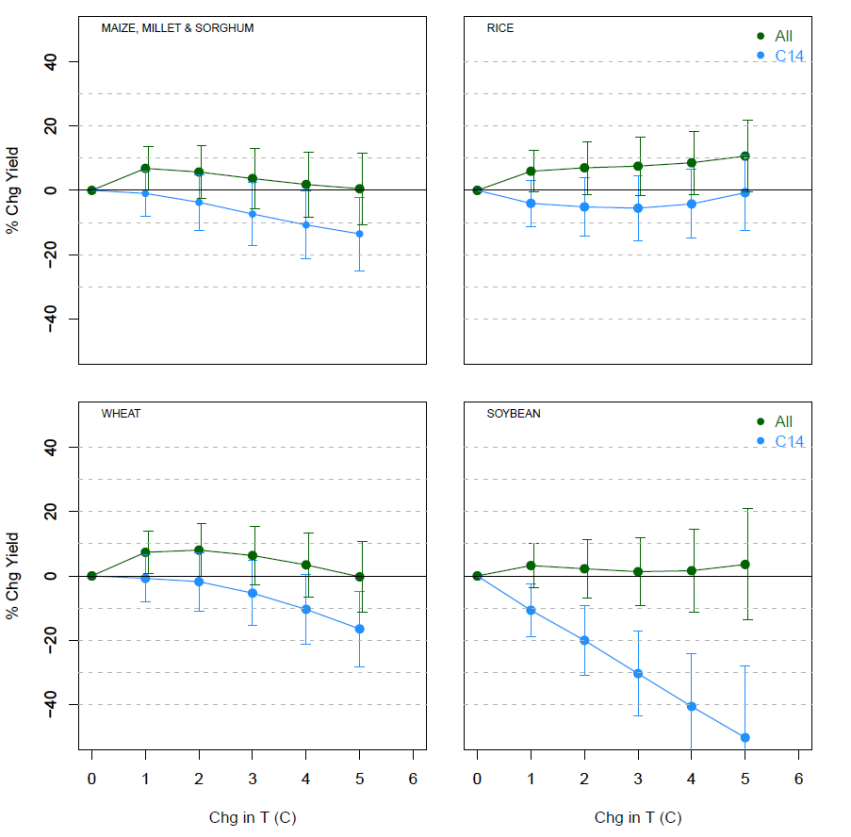
\includegraphics[width=0.9\textwidth]{bilder/bilderKlima-0079.png}\\[1cm]
\end{center}
\caption{Ernteerträge unter CO$_2$-induzierter Klimaerwärmung. Blau: wie veröffentlicht in Moore et
al. (2017). Grün: nach Einbeziehung ausgelassener Daten. Quelle: McKitrick (2025).}
\end{figure}

McKitrick (2025) untersuchte die Datenbank von Moore et al. erneut und fand heraus, dass sie, obwohl sie behauptete, 1.722 Studien zu umfassen, nur die Hälfte der Einträge (N=862) vollständige Aufzeichnungen hatte, sodass die für die Regressionsanalyse verfügbare Stichprobe viel kleiner war als beide Studien angaben. McKitrick bemerkte, dass die am häufigsten fehlenden Aufzeichnungen die Veränderungen des Umgebungs-CO$_2$ waren und fand heraus, dass diese in vielen Fällen aus den zugrundeliegenden Studien oder den ursprünglichen Klimaszenarientabellen wiedergewonnen werden konnten, wodurch die verwendbare Stichprobengröße um 40 Prozent erhöht wurde. Die Nutzpflanzenertragsprojektion unter Einbeziehung der neu verfügbaren Daten veränderte sich erheblich. Wie in Abbildung 9.2 gezeigt, implizierte der partielle Datensatz, dass Erwärmung den Ertrag verringern würde (blaue Linien), während der vollständige Datensatz konstante oder steigende globale Erträge implizierte, sogar bis zu \SI{5}{\celsius} Erwärmung (grüne Linien).


\section{CO$_2$-Düngung und Nährstoffverlust}
Belege haben gezeigt, dass CO$_2$-induzierte Biomassegewinne manchmal von Reduzierungen der Konzentrationen von Protein und anderen Schlüsselnährstoffen wie Eisen und Zink begleitet werden (Ebi et al. 2021). Einige Experimente haben gezeigt, dass die steigenden Temperaturen, die erwartungsgemäß höhere CO$_2$-Konzentrationen begleiten, diesen Verlust ausgleichen werden (Köhler et al. 2019), obwohl die Belege dafür gemischt sind, ebenso wie die Belege dafür, dass die bis heute beobachtete Nährstoffverdünnung vollständig höherem CO$_2$ zuzuschreiben ist (Ziska 2022). Falls Nährstoffverdünnung unter steigenden CO$_2$-Konzentrationen auftritt, gibt es mehrere adaptive Strategien, die verfolgt werden könnten.

Erstens ist selektive Züchtung zur Erhöhung des Mikronährstoffgehalts bereits etabliert (Saltzman et al. 2017) und hat sich als kosteneffektive agronomische Strategie erwiesen (Ebi et al. 2021). Strategien können sowohl konventionelle Züchtung als auch genetisch veränderte Organismen einschließen. Ein Beispiel für letzteres ist Golden Rice, das erhöhte Konzentrationen von Beta-Carotin enthält, um die Biosynthese von Vitamin A im menschlichen Körper zu verstärken. Optimale Strategien werden standortspezifisch sein, weil sie je nach Nutzpflanze, Klima und Bodentyp variieren (Ebi et al. 2021).
Zweitens ist die Anreicherung von Lebensmittelprodukten mit Mikronährstoffen bereits Routine. Folsäure (ein B-Vitamin) wird Mehl und vielen anderen Lebensmitteln zugesetzt; Jod wird Kochsalz zugesetzt, die meisten kommerziellen Frühstückszerealien sind mit Eisen und zahlreichen Vitaminen angereichert, usw. Drittens sind Nahrungsergänzungsmittel in Form von Multivitamintabletten preiswert, weit verfügbar und werden routinemäßig konsumiert.

Eine Sorge über die Abhängigkeit von adaptiven Strategien ist, ob sie in einkommensschwachen Ländern machbar sind. Mikronährstoffmangel ist bereits ein Problem in der Entwicklungswelt und Nahrungsergänzungsmittel haben sich als effektive kostengünstige Antwort erwiesen (Ebi et al. 2021). Es sollte auch bemerkt werden, dass die IPCC-Emissionsszenarien, die hohe Erwärmungsgrade generieren, auch starkes Einkommenswachstum beinhalten. Die SSP-Szenarien nehmen an\footnote{Siehe Zusammenstellung unter Our World in Data.}, dass im Vergleich zu 2005er Niveaus das globale Pro-Kopf-Einkommen bis 2100 im niedrigsten Wachstumsfall (SSP3) sich verdoppeln wird, und im höchsten Emissionsfall (SSP5) wird das globale Pro-Kopf-Einkommen um fast das 16-fache wachsen. In diesem Szenario enden sogar die ärmsten Regionen (Afrika und der Mittlere Osten) mit einem Pro-Kopf-Einkommen von etwa US\$126.000, 70 Prozent höher als das aktuelle US-Pro-Kopf-Einkommen (etwa US\$75.000). Folglich sind dieselben Szenarien, in denen CO$_2$-Konzentrationen am meisten steigen, auch jene, in denen globale Armut weitgehend eliminiert wird, in welchem Fall alle Länder in der Lage wären, sich Nahrungsergänzungsmittel zu leisten, die nötig sind, um Mikronährstoffmangel zu beheben, falls er auftritt und nicht durch landwirtschaftliche Strategien auf dem Betrieb behoben werden kann.

Zusammenfassend gibt es reichliche Belege, die Jahrzehnte zurückreichen, dass steigende CO$_2$-Konzentrationen Pflanzen zugutekommen, einschließlich landwirtschaftlicher Nutzpflanzen, und dass CO$_2$-induzierte Erwärmung ein Nettonutzen für die US-Landwirtschaft sein wird. Soweit Nährstoffverdünnung auftritt, stehen mildernde Strategien zur Verfügung, die erforscht und an lokale Bedingungen angepasst werden müssen.

\vfill
\noindent\textbf{Literaturverzeichnis:}

\begingroup
\parindent=0pt
\everypar{\hangindent=2em\hangafter=1\relax}

Ainsworth, Elizabeth and Stephen P. Long (2020) 30 years of free-air carbon dioxide enrichment (FACE):
What have we learned about future crop productivity and its potential for adaptation? Global Change
Biology https://doi.org/10.1111/gcb.15375

Allen Jr, L. K. (2011). Elevated CO2 increases water use efficiency by sustaining photosynthesis of water-
limited maize and sorghum. Journal of Plant physiology, 168(16), 1909-1918.

Bareille, F. and R. Chakir (2023) The impact of climate change on agriculture: A repeat-Ricardian analysis.
Journal of Environmental Economics and Management 119

Blandino, M. B. (2020). Elevated CO2 impact on common wheat (Triticum aestivum L.) yield, wholemeal
quality, and sanitary risk. Journal of agricultural and food chemistry, 68(39), 10574-10585.

Burke, Marshall and Kyle Emerick (2016) Adaptation to Climate Change: Evidence from US Agriculture.
American Economic Journal: Economic Policy 8(3) August 2016 106—140
https://www.aeaweb.org/articles?id=10.1257/pol.20130025

Cheng, L., Zhang, L., Wang, YP. et al. Recent increases in terrestrial carbon uptake at little cost to the water
cycle. Nature Communications 8, 110 (2017). https://doi.org/10.1038/s41467-017-00114-5

CO2Science.org (undated) Plant growth archive \url{http://www.co2science.org/data/plant_growth/dry/dry_subject_b.php}

Deryng, D., Elliott, J., Folberth, C. et al. (2021) Regional disparities in the beneficial 
effects of rising
CO2 concentrations on crop water productivity. Nature Climate Change 6, 786–790 (2016).
https://doi.org/10.1038/nclimate2995

Deschênes, Olivier and Michael Greenstone (2012) The Economic Impacts of Climate Change: Evidence
from Agricultural Output and Random Fluctuations in Weather: Reply to Comment American
Economic Review. 102, no. 7: 3761-3773. http://hdl.handle.net/1721.1/82641

Ebi, Kristie L, C Leigh Anderson, Jeremy J Hess, et al. (2021) Nutritional quality of crops in a high CO2
world: an agenda for research and technology development. Environmental Research Letters 16(6)
064045 https://iopscience.iop.org/article/10.1088/1748-9326/abfcfa

Köhler, Iris H., Steven C. Huber, Carl J. Bernacchi, Ivan R. Baxter (2019) Increased temperatures may
safeguard the nutritional quality of crops under future elevated CO2 concentrations. The Plant Journal
97(5) 872 – 886 https://onlinelibrary.wiley.com/doi/epdf/10.1111/tpj.14166

Li, D. L. (2013). Effects of elevated CO2 on the growth, seed yield, and water use efficiency of soybean
(Glycine max (L.) Merr.) under drought stress. Agricultural Water Management, 129, 105-112.

McKitrick, Ross R. (2025) Extended Crop Yield Meta-analysis Data do not Support Upward SCC Revision.
Scientific Reports 15 article 5575 https://www.nature.com/articles/s41598-025-90254-2

Mendelsohn, R., Nordhaus, W. D., \& Shaw, D. (1994). The impact of global warming on agriculture: a
Ricardian analysis. The American Economic Review, Sept 1994 753-771.

Moore FC, Baldos U, Hertel T, Diaz D (2017) New science of climate change impacts on agriculture implies
higher social cost of carbon. Nature Communications 8:1607. https://doi. org/10. 1038/s41467-017-
01792-x

Ortiz-Bobea, Ariel (2019) The role of nonfarm influences in ricardian estimates of climate change impacts
on US agriculture. American Journal of Agricultural Economics. 102 (3), 934–959.

Saltzman, Amy, Ekin Birol, Adewale Oparinde et al. (2017) Availability, production, and consumption of
crops biofortified by plant breeding: current evidence and future potential. Annals of the New York
Academy of Sciences Volume 1390, Issue1 \url{https://doi.org/10.1111/nyas.13314}

Schlenker, Wolfram and Michael Roberts (2009) Nonlinear temperature effects indicate severe damages to
U.S. crop yields under climate change. Proceedings of the National Academy of Sciences
106 (37) 15594-15598 \url{https://doi.org/10.1073/pnas.0906865106}

Taylor, Charles and Wolfram Schlenker (2023) Environmental drivers of agricultural productivity growth:
CO2 fertilization of US field crops. National Bureau of Economic Research Working paper 29320,
https://www.nber.org/papers/w29320

US Environmental Protection Agency (2023) Supplementary Material for the Regulatory Impact Analysis
for the Final Rulemaking, “Standards of Performance for New, Reconstructed, and Modified Sources
and Emissions Guidelines for Existing Sources: Oil and Natural Gas Sector Climate Review”, EPA
Report on the Social Cost of Greenhouse Gases: Estimates Incorporating Recent Scientific Advances,
Nov. 2023, \url{https://www.epa.gov/system/files/documents/2023-12/epa_scghg_2023_report_final.pdf}

Zhang et al. (2024) Less than 4\% of dryland areas are projected to desertify despite increased aridity under
climate change. Nature Communications Earth and Environment 5 June 2024
\url{https://www.nature.com/articles/s43247-024-01463-y}

Ziska, Lewis H (2022) Rising Carbon Dioxide and Global Nutrition: Evidence and Action Needed. Plants
1(7), 1000; \url{https://doi.org/10.3390/plants11071000}

\endgroup


\cleardoublepage
\chapter{BEWÄLTIGUNG VON RISIKEN EXTREMER WETTEREREIGNISSE}
\paragraph{Kapitelzusammenfassung}
\begin{quote}
Trends bei Schäden durch extreme Wetterereignisse und klimatische Ereignisse werden durch Bevölkerungszunahme und Wirtschaftswachstum dominiert. Technologische Fortschritte wie verbesserte Wettervorhersagen und Frühwarnsysteme haben die Verluste durch extreme Wetterereignisse erheblich reduziert. Bessere Bauvorschriften, Hochwasserschutz und Katastrophenschutzmechanismen haben die wirtschaftlichen Verluste relativ zum BIP gesenkt. Die Expansion der US-Wirtschaft hat die relative Auswirkung von Katastrophenkosten verwässert, wie im Vergleich der historischen und modernen BIP-Prozentsätze zu sehen ist. Das Mortalitätsrisiko durch Hitze ist aufgrund von Anpassungsmaßnahmen erheblich gesunken, einschließlich der Einführung von Klimaanlagen, die auf die Verfügbarkeit bezahlbarer Energie angewiesen ist. Die US-Mortalitätsrisiken steigen selbst unter extremen Erwärmungsszenarien voraussichtlich nicht an, wenn Menschen in der Lage sind, Anpassungsmaßnahmen zu ergreifen.
\end{quote}

\section{Sozioökonomischer Kontext}
Risiken durch anthropogenen Klimawandel werden von natürlicher Wetter- und Klimavariabilität beeinflusst und durch die Exposition von Vermögenswerten in küstennahen und anderen katastrophengefährdeten Regionen sowie durch Vulnerabilitäten ärmerer Bevölkerungsgruppen dominiert. Die Entwicklung des Klimarisikos in den USA wurde von gesellschaftlichen Faktoren dominiert, eher als von Veränderungen der tatsächlichen Wetter- und Klimagefahren. Todesfälle durch Wetterkatastrophen sind seit 1900 erheblich zurückgegangen, obwohl die US-Bevölkerung von 76 Millionen im Jahr 1900 auf über 331 Millionen im Jahr 2020 gewachsen ist (Goklany 2011). Zum Beispiel tötete der Galveston-Hurrikan über 8.000 Menschen im Jahr 1900 (0,01 Prozent der US-Bevölkerung), wohingegen die schlimmste jüngere Katastrophe, Hurrikan Katrina im Jahr 2005, 1800 Menschen tötete (oder 0,0006 Prozent der US-Bevölkerung) (NOAA National Hurricane Center 2025; U.S. Census Bureau 2025).

Technologische Fortschritte haben Verluste durch extreme Wetterereignisse erheblich reduziert. Frühwarnsysteme, Satellitenüberwachung und verbesserte Wettervorhersagen haben Todesfälle reduziert, obwohl genaue Zahlen schwer zu quantifizieren sind (Deryugina und Hsiang 2023). US-Wettervorhersagen wurden dahingehend geschätzt, dass sie Verluste durch Wetterereignisse mit einem jährlichen Nutzen von 31,5 Milliarden US-Dollar reduzieren, indem sie Leben und Eigentum schützen und Landwirtschaft und Transport unterstützen (NRC 2010). Verbesserte Hurrikan-Vorhersagen haben die Ausgaben vor und nach dem Landfall reduziert, mit geschätzten jährlichen Kostenreduktionen pro Hurrikan von 5 Milliarden US-Dollar (Molina und Rudik 2024).

Infrastrukturverbesserungen haben zu erheblichen Reduktionen der Verluste durch extreme Wetterereignisse beigetragen. Bauvorschriften, wie die in Florida nach Hurrikan Andrew (1992) implementierten, haben Verluste reduziert, indem sie sicherstellen, dass Strukturen starken Winden und Überschwemmungen widerstehen können. Nach 2002 gebaute Häuser zeigten minimale Schäden während Hurrikan Michael (2018), im Gegensatz zu älteren Häusern (FEMA 2020). Ufermauern wie die Galveston Seawall schützen vor Wellenwirkung und Sturmfluten. Das New Orleans Hurricane and Storm Damage Risk Reduction System milderte erfolgreich die Sturmflut während Hurrikan Isaac (2012) (Battelle Memorial Institute 2013). Staudämme im Inland der USA helfen dabei, Überschwemmungen zu kontrollieren, indem sie überschüssiges Wasser während starker Regenfälle speichern. Es wird geschätzt, dass die Tennessee Valley Authority (TVA)-Staudämme etwa 309 Millionen US-Dollar jährliche Hochwasserschäden in der TVA-Region und entlang der Ohio- und Mississippi-Flüsse verhindern (TVA, 2025). Während Hurrikan Helene (2024) verhinderten die TVA-Strategien ungefähr 406 Millionen US-Dollar an potentiellen Schäden (APPA 2024).

\section{Datenherausforderungen}
Seit 1980 stellt NOAA eine Zählung jährlicher wetterbedingte Katastrophen in den USA bereit, von denen geschätzt wird, dass sie 1 Milliarde US-Dollar (inflationsbereinigt) überschritten haben, was einen erheblichen Anstieg ab 2008 zeigt. NOAA und andere Regierungsbeamte haben den Aufwärtstrend in der Billion-Dollar-Katastrophen-Serie als Beleg dafür angeführt, dass der Klimawandel extremes Wetter verschlimmert (Pielke Jr., 2024). Aber über die Zeit sind Bevölkerung und Wohlstand in den USA dramatisch gestiegen, sodass wenn ein extremes Wetter- oder Klimaereignis auftritt, es mehr Schäden gibt, selbst wenn es keinen zugrundeliegenden Trend in der Häufigkeit oder Intensität extremen Wetters gibt. Pielke Jr. (2024) zeigt, dass Verluste pro Wetterkatastrophe als Anteil des BIP seit 1980 um etwa 80 Prozent abgenommen haben, wie in Abbildung 10.1 gezeigt. Pielke Jr. (2024) argumentierte auch, dass NOAA zusätzlich zum Verlass auf undurchsichtige Datenquellen und nicht gemeldete Anpassungen versäumt hat, seine Billion-Dollar-Katastrophen-Datenserie ordnungsgemäß für Veränderungen in Bevölkerungsexposition und Wohlstand zu normalisieren. Im Mai 2025 gab NOAA bekannt, dass es das Trillion-Dollar-Katastrophen-Produkt aus der Veröffentlichung zurückgezogen hat (Pielke Jr., 2025).


\begin{figure}[H]
\begin{center}
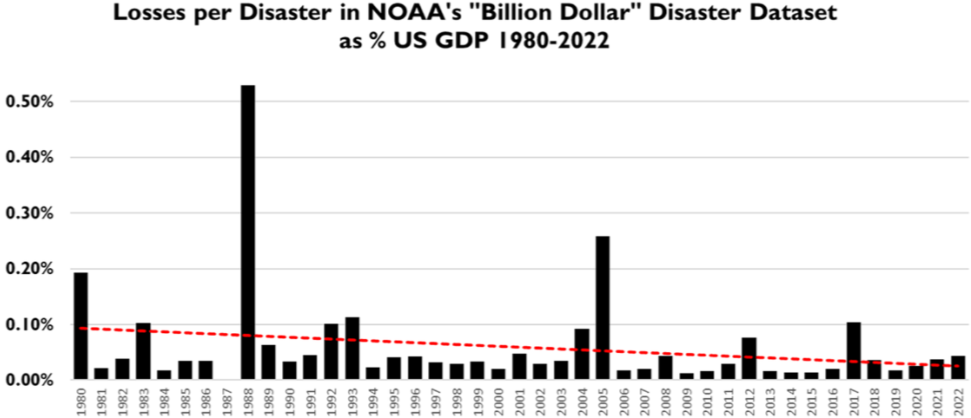
\includegraphics[width=0.9\textwidth]{bilder/bilderKlima-0080.png}\\[1cm]
\end{center}
\caption{Verluste pro Katastrophe als \% des Bruttoinlandsprodukts in NOAAs Milliarden-Dollar-Katastrophen-Datensatz (die im Juli 2023 heruntergeladene Version), 1980 bis 2022. Quelle: (Pielke, Jr. 2024)}
\end{figure}
 
Zusammenfassend werden Trends bei Verlusten durch extreme Wetter- und Klimaereignisse von Bevölkerungszunahmen und Wirtschaftswachstum dominiert. Technologische Fortschritte wie verbesserte Wettervorhersagen und Frühwarnsysteme haben Verluste durch extreme Wetterereignisse erheblich reduziert. Bessere Bauvorschriften, Hochwasserschutz und Katastrophenschutzmechanismen haben wirtschaftliche Verluste relativ zum BIP gesenkt. Schließlich hat die Expansion der US-Wirtschaft die relative Auswirkung von Katastrophenkosten verwässert, wie im Vergleich der historischen und modernen BIP-Prozentsätze zu sehen ist.

\section{Mortalität durch Temperaturextreme}
\subsection{Hitze- und Kälterisiken}
Veränderungen bei Temperaturextremen gehören zu den sichersten Auswirkungen, die in einer sich erwärmenden Welt erwartet werden. Es liegt nahe, dass extreme Hitzeereignisse wahrscheinlich häufiger werden würden, während extreme Kälteereignisse seltener werden würden. Dieses Muster ist in der historischen Periode evident, jedoch nicht in den kontinentalen USA (Kapitel 6), und es wird erwartet, dass es sich bei weiterer Erwärmung fortsetzt.

Mortalität während Hitzeextremen wird typischerweise durch Hitzschlag und Hitzeerschöpfung verursacht, während Mortalität während Kälteextremen typischerweise von Unterkühlung und Herzbelastung herrührt. Die globale Mortalität ist erheblich größer für kalte Bedingungen als für heiße Bedingungen (Zhao et al 2021, Ritchie 2024). Anders als bei hitzebezogener Mortalität setzen kältewetterbedingte Risiken sogar bei mäßig kalten Bedingungen ein (Gasparini et al. 2015, Lee und Dessler 2023). Die US-EPA (unter Berufung auf Daten der Centers for Disease Control) berichtet, dass im Durchschnitt von 1999 bis 2015 2,2 Todesfälle pro Million Amerikaner auftraten, bei denen Kälte als Hauptursache aufgeführt wurde, und zusätzliche 2,4 Todesfälle pro Million, bei denen Kälte als beitragender Faktor aufgeführt wurde (EPA 2025). Im Gegensatz dazu gab es 1,3 Todesfälle pro Million, bei denen Hitze die Hauptursache war, und zusätzliche 0,8 pro Million, bei denen sie ein beitragender Faktor war. Nach dieser Messgröße verursacht Kälte etwa doppelt so viele wetterbezogene Todesfälle wie Hitze.

Epidemiologische Methoden, die Korrelationsbelege berücksichtigen, nicht nur Sterbeurkunden-Berichte, deuten darauf hin, dass das Kälte/Wärme-Verhältnis viel höher sein könnte. Eine 13-Länder-Studie von 74 Millionen Todesfällen von 1985 bis 2012 schätzte, dass im Durchschnitt 7,7 Prozent der Todesfälle suboptimalen Temperaturen zugeschrieben werden konnten, von denen 7,4 Prozent der Kälte und nur 0,4 Prozent der Hitze zugeschrieben wurden (Gasparini et al. 2015). Mit anderen Worten tötete kaltes Wetter 18,5-mal so viele Menschen wie heißes Wetter.

Abbildung 10.2 zeigt die Verteilung der Ergebnisse von Gasparini et al. (2015) nach Ländern. Für die Vereinigten Staaten betrug der Anteil der Todesfälle, die der Temperatur zugeschrieben wurden, 5,9 Prozent, von denen 5,5 Prozent auf Kälte zurückzuführen waren, sodass kaltes Wetter 14-mal so viele Menschen tötete wie heißes Wetter.

\begin{figure}[H]
\begin{center}
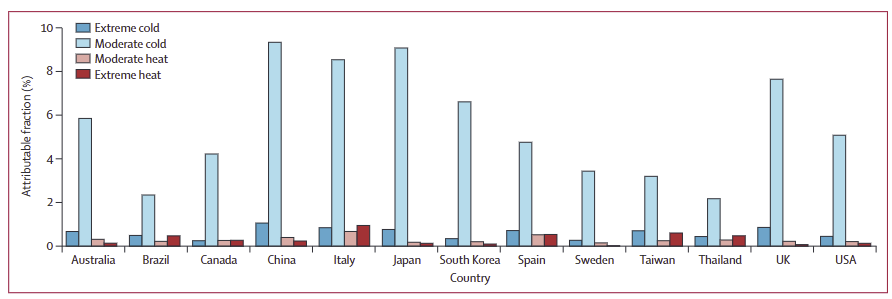
\includegraphics[width=0.9\textwidth]{bilder/bilderKlima-0081.png}\\[1cm]
\end{center}
\caption{Mortalität zugeschrieben extremer und mäßiger Kälte und Hitze nach Ländern. Quelle: reproduziert von Gasparini et al. (2015).}
\end{figure}

Es gibt starke Belege dafür, dass sich Menschen an Wetterrisiken anpassen. Lee und Dessler (2023) berichteten, dass 86 Prozent der temperaturbezogenen Todesfälle in 40 US-Städten auf kältebezogene Mortalität zurückzuführen waren und dass aufgrund von Anpassung das relative Todesrisiko sowohl in heißen als auch in kalten Städten abnahm, als die saisonalen Temperaturen anstiegen. Allen und Sheridan (2018) fanden, dass kurze, frühe Kälteereignisse 2- bis 5-mal tödlicher waren als Hitzeereignisse, aber das Mortalitätsrisiko sowohl bei Kälte- als auch bei Hitzeextremen auf nahezu null fällt, wenn die Ereignisse spät in der Saison auftreten.

Davis et al. (2003) untersuchten hitzebezogene Mortalität in 28 US-Städten von den 1960er Jahren bis zum Ende der 1990er Jahre und fanden, dass hitzebezogene Mortalität über den Stichprobenzeitraum um drei Viertel abnahm. Bobb et al. (2014) untersuchten Mortalitätsdaten für 106 Millionen Menschen in über 100 US-Städten und fanden einen 60-prozentigen Rückgang der durchschnittlichen hitzebezogenen Mortalität über den Zeitraum 1987-2005, von 51 pro tausend Todesfälle auf 19. Sie fanden außerdem, dass der größte Rückgang bei Senioren über 75 Jahren auftrat. In einer Studie von 42 Millionen Todesfällen in 211 US-Städten von 1962 bis 2006 fanden Nordio et al. (2015) einen mehr als 90-prozentigen Rückgang des Mortalitätsrisikos durch übermäßige Hitze.

Im Kontext großer Rückgänge hitzebezogener Mortalität sind steigende Temperaturen mit einer Nettoeinsparung von Menschenleben verbunden, da sie die Mortalität durch Kälteereignisse reduzieren. AR6 Working Group 2 Kapitel 16.2.3.5 (O'Neill et al. 2022) erkennt an, dass das hitzebezogene Mortalitätsrisiko über die Zeit abnimmt:

\begin{quote}
Hitzezuschreibbare Mortalitätsfraktionen sind über die Zeit in den meisten Ländern aufgrund allgemeiner Verbesserungen der Gesundheitssysteme, zunehmender Verbreitung von Wohnklimaanlagen und Verhaltensänderungen zurückgegangen. Diese Faktoren, die die Anfälligkeit der Bevölkerung für Hitze bestimmen, haben über den Einfluss von Temperaturveränderungen überwogen.
\end{quote}

Doch das IPCC stellt die Gesamtsituation in seinem AR6-Synthesebericht falsch dar. Abschnitt A.2.5 dieses Dokuments besagt: \emph{In allen Regionen haben Zunahmen bei extremen Hitzeereignissen zu menschlicher Mortalität und Morbidität geführt (sehr hohes Vertrauen).} Aber es schweigt über den größeren Rückgang der Todesfälle während extremer Kälteereignisse.


Der beobachtete Rückgang hitzebezogener Mortalität in den USA wurde spezifisch der Anpassung zugeschrieben. Wang et al. (2018) nutzten die räumliche Variabilität hitzewellenbezogener Mortalität in 209 US-Städten von 1962 bis 2006. Während einfache Korrelation eine Zunahme des Mortalitätsrisikos während Hitzewellen zu implizieren schien, führte die Berücksichtigung der Anpassung an Hitzewellenintensität dazu, dass der Effekt auf nahezu null fiel und statistisch unbedeutend wurde. Sie verwendeten die Ergebnisse ihres epidemiologischen Modells, um hitzebezogene Mortalität bis 2050 unter vier RCP-Erwärmungsszenarien (einschließlich RCP8.5) mit und ohne adaptives Verhalten zu projizieren. Unter der Annahme, dass Menschen sich weiterhin an die Hitzewellenrisiken in den Regionen anpassen, in denen sie leben, projizieren Wang et al. (2018) nicht nur keine Zunahme hitzebezogener Mortalität, sondern eine allgemeine Mortalitätsabnahme für die USA. Sie schlussfolgern, dass

\begin{quote}
Die Ignorierung der Anpassung würde zu einer erheblichen Überschätzung zukünftiger hitzewellenbezogener Mortalität führen... Unter Berücksichtigung der Anpassung würde sich die allgemeine hitzebezogene Mortalität bis 2050 nicht erheblich über die Zeit im Vergleich zu 2006 ändern.
\end{quote}

\subsection{Mortalitätsrisiken und Energiekosten}
Eine 2016-Studie zu langfristigen Mortalitätsrisiken in den USA im Zusammenhang mit Temperaturschwankungen (Barreca et al. 2016) zeigte, dass Zunahmen der Mortalität in den USA sowohl mit kaltem als auch mit heißem Wetter verbunden sind. Aber über die Zeit reduzierten die Einführung von Elektrizität und die Einführung von Zentralheizung und Klimaanlage (AC) beide Risiken dramatisch, besonders jene, die mit heißem Wetter verbunden sind. Vor 1960 fügte ein Tag über \SI{90}{F} (\SI{32}{\celsius}) 2.2 Prozent zur durchschnittlichen Mortalitätsrate hinzu, aber nach 1960 fügte dasselbe Wetter nur 0.3 Prozent zum Mortalitätsrisiko hinzu, eine 85-prozentige Reduktion. Vor 1960 fügten Temperaturen unter \SI{39}{F} (\SI{4}{\celsius}) etwa 1 Prozent zum Mortalitätsrisiko hinzu, aber nach 1960 fügte dasselbe Wetter nur etwa die Hälfte dieser Menge hinzu. Anpassung durch konventionelle Haushaltsverbesserungen reduzierte die öffentliche Vulnerabilität gegenüber Wetterextremen dramatisch. Die gesamte Reduktion der Heißwetter-Mortalität war der weit verbreiteten Einführung von Innen-Klimaanlagen zuzuschreiben, die von der Verfügbarkeit zuverlässiger und bezahlbarer Elektrizität abhing.

Die Folgerung aus diesem Befund ist, dass die Verwendung von Heizungs- und Kühlsystemen davon abhängt, dass Energie bezahlbar ist. Doremus et al. (2022) zeigten, dass wohlhabende und arme Haushalte in den USA ihre Energieausgaben bei moderaten Temperaturschwankungen mit ähnlichen Raten anpassen, aber nicht bei extremen Temperaturschwankungen. Wenn Temperaturen auf sehr kalte Werte schwanken (< \SI{5}{\celsius}) steigen die Energieausgaben in Haushalten mit hohem Einkommen um 1.2 Prozent, aber in Haushalten mit niedrigem Einkommen nur um 0,5 Prozent. An sehr heißen Tagen (>\SI{30}{\celsius}) steigen die Stromausgaben in Haushalten mit hohem Einkommen um 0.5 Prozent, ändern sich aber in Haushalten mit niedrigem Einkommen überhaupt nicht. Das letztere Ergebnis wird sogar in Teilstichproben beobachtet, wo alle Haushalte Klimaanlagen haben. Cong et al. (2022) berichten ähnliche Befunde für eine Stichprobe von Haushalten in Arizona. Die Implikation ist, dass selbst bei weit verbreiteter Einführung von Hausheizungs- und -kühlsystemen die Unfähigkeit, sich Energie zu leisten, einkommensschwache Haushalte Wetterextremen aussetzt.

\vfill
\noindent\textbf{Literaturverzeichnis:}

\begingroup
\parindent=0pt
\everypar{\hangindent=2em\hangafter=1\relax}

Allen, M.J. and S.C. Sheridan (2018) Mortality risks during extreme temperature events (ETEs) using a
distributed lag non-linear model. (2018) International Journal of Biometeorology 62, 57–67 (2018).
\url{https://doi.org/10.1007/s00484-015-1117-4}

American Public Power Association. (APPA, 2024, March 7). TVA flood mitigation strategies prevented
approximately \$406 million in potential damages. Public Power Current.
\url{https://www.publicpower.org/periodical/article/tva-flood-mitigation-strategies-prevented-
approximately-406-million-potential-damages}

Barreca, Alan, Karen Clay, Olivier Deschenes, Michael Greenstone, and Joseph S Shapiro (2016), Adapting
to climate change: The remarkable decline in the US temperature mortality relationship over the
twentieth century, Journal of Political Economy, 2016, 124 (1), 105–159.

Battelle Memorial Institute. (2013, December). Final independent external peer review report: Hurricane
Isaac (2012) assessment (Prepared for U.S. Army Corps of Engineers, New Orleans District).
\url{https://www.mvn.usace.army.mil/Portals/56/docs/PD/PeerReview/TCN13-
003HurrIsaacAssessIEPRFinal.pdf}

Bobb JF, RD Peng, ML Bell and F Dominici (2014) Heat-related mortality and adaptation to heat in the
United States. Environmental Health Perspectives 122:811–816;
\url{https://ehp.niehs.nih.gov/doi/full/10.1289/ehp.1307392}

Cong, S., D. Nock, Y.L. Qiu, Y.L. et al. Unveiling hidden energy poverty using the energy equity
gap. Nature Communications 13, 2456 (2022). \url{https://doi.org/10.1038/s41467-022-30146-5}

Davis, Robert E., Paul C. Knappenberger, Patrick J. Michaels and Wendy M. Novicoff (2003) “Changing
Heat-Related Mortality in the United States” Environmental Health Perspectives 111(14) November
2003 pp. 1712—1718 \url{https://ehp.niehs.nih.gov/doi/pdf/10.1289/ehp.6336}

Deryugina, T., \& Hsiang, S. M. (2023). Does the environment still matter? Daily temperature and income
in the United States (NBER Working Paper No. 31361). National Bureau of Economic Research.
\url{https://www.nber.org/papers/w31361}

Doremus, JM, I. Jacqz and S. Johnston (2022), “Sweating the energy bill: Extreme weather, poor
households, and the energy spending gap.” Journal of Environmental Economics and Management,
doi: \url{https://doi.org/10.1016/j.jeem.2022.102609} .

Environmental Protection Agency (2025) Climate Change Indicators. \url{https://www.epa.gov/climate-
indicators/view-indicators}

Federal Emergency Management Agency (FEMA). (2020, February 13). The role of Florida’s building
codes in Hurricane Michael recovery. \url{https://www.fema.gov/case-study/role-floridas-building-codes-
2018-hurricane-michael}

Gasparini, A., Y. Guo, M. Hashizume et al. (2015) Mortality risk attributable to high and low ambient
temperature: a multicountry observational study. The Lancet 386: 369-385 July 25, 2015
\url{http://dx.doi.org/10.1016/S0140-6736(14)62114-0}

Goklany, I. M. (2011). Deaths from extreme weather events, 1900–2010. Reason Foundation.
\url{https://a8d50b36.delivery.rocketcdn.me/wp-
content/uploads/2011/09/deaths_from_extreme_weather_1900_2010.pdf}

Lee, Jangho and Andrew Dessler (2023) Future Temperature-Related Deaths in the U.S.: The Impact of
Climate Change, Demographics, and Adaptation. GeoHealth 7(8) August 2023
\url{https://doi.org/10.1029/2023GH000799}

Molina, R and I Rudik (2024) The value of improving hurricane forecasts. National Bureau of Economic
Research Working Paper 32548 June 2024. \url{https://www.nber.org/digest/202409/value-improving-
hurricane-forecasts}

National Hurricane Center. (n.d.). Costliest U.S. tropical cyclones tables updated. NOAA National
Hurricane Center. Retrieved May 8, 2025, from \url{https://www.nhc.noaa.gov/outreach/history/}
National Research Council. (2010). Adapting to the impacts of climate change. The National Academies
Press. \url{https://nap.nationalacademies.org/read/12888/chapter/2}

Nordio, Francesco, Antonella Zanobetti, Elena Colicino, Itai Kloog and Joel Schwartz (2015). “Changing
patterns of the temperature–mortality association by time and location in the US, and implications for
climate change” Environment International Volume 81, pp 80-86
\url{https://doi.org/10.1016/j.envint.2015.04.009.}

O'Neill, B., et al. (2022). Key risks across sectors and regions. In AR6 Working Group II Climate Change
2022: Impacts, Adaptation and Vulnerability (pp. 2411–2538). Intergovernmental Panel on Climate
Change. www.ipcc.ch

Pielke Jr., R. (2024). Scientific integrity and U.S. 'billion dollar disasters'. npj Natural Hazards, 1, Article
12. \url{https://www.nature.com/articles/s44304-024-00011-0}

Pielke Jr., R. (2025, May 8). RIP NOAA's billion dollar disasters. The Honest Broker [Substack].
\url{https://rogerpielkejr.substack.com/p/rip-noaas-billion-dollar-disasters}

Ritchie, H. (2024). How many people die from extreme temperatures, and how this could change in the
future: Part one. Our World in Data. \url{https://ourworldindata.org/part-one-how-many-people-die-from-
extreme-temperatures-and-how-could-this-change-in-the-future}

Tennessee Valley Authority (TVA). (n.d.). Flood management. Retrieved May 8, 2025, from
\url{https://www.tva.com/environment/managing-the-river/flood-management}

U.S. Census Bureau. (n.d.). Decennial census by decade. Retrieved May 8, 2025, from
https://www.census.gov/programs-surveys/decennial-census/decade.html

Wang, Yan, Francesco Nordio , John Nairn , Antonella Zanobetti and Joel D. Schwartz (2018) \emph{Accounting
for adaptation and intensity in projecting heat wave-related mortality} Environmental Research 161 pp.
464—471. \url{https://doi.org/10.1016/j.envres.2017.11.049}

Zhao, Q., et al. (2021). Global, regional, and national burden of mortality associated with non-optimal
ambient temperatures from 2000 to 2019: A three-stage modelling study. The Lancet Planetary
Health, 5(7). \url{https://doi.org/10.1016/s2542-5196(21)00081-4}

\endgroup

\cleardoublepage
\chapter{KLIMAWANDEL, WIRTSCHAFT UND DIE SOZIALEN KOSTEN VON KOHLENSTOFF}
\paragraph{Kapitelzusammenfassung}
\begin{quote}
Ökonomen haben das Klima lange als relativ unwichtigen Faktor für das Wirtschaftswachstum betrachtet, eine Ansicht, die vom IPCC selbst im AR5 geteilt wird. Die Mainstream-Klimaökonomie hat anerkannt, dass CO$_2$-induzierte Erwärmung einige negative wirtschaftliche Auswirkungen haben könnte, aber sie sind zu gering, um eine aggressive Minderungspolitik zu rechtfertigen, und der Versuch, die globale Erwärmung zu "stoppen" oder zu begrenzen, selbst auf Ebenen weit über dem Pariser Ziel, wäre schlimmer als nichts zu tun. Eine einflussreiche Studie von 2012 legte nahe, dass globale Erwärmung dem Wachstum in armen Ländern schaden würde, aber der Befund hat sich anschließend als nicht robust erwiesen. Studien, die Modellierungsunsicherheiten vollständig berücksichtigen, finden entweder keine Belege für einen negativen Effekt auf das globale Wachstum durch CO$_2$-Emissionen oder finden arme Länder ebenso wahrscheinlich profitierend wie reiche Länder.

Schätzungen der sozialen Kosten von Kohlenstoff (SCC) sind höchst unsicher aufgrund von Unbekannten im zukünftigen Wirtschaftswachstum, sozioökonomischen Pfaden, Diskontierungsraten, Klimaschäden und Systemreaktionen. Die SCC ist nicht intrinsisch informativ bezüglich der wirtschaftlichen oder gesellschaftlichen Auswirkungen des Klimawandels. Sie bietet einen Index, der große Netzwerke von Annahmen über das Klima und die Wirtschaft mit einem Dollarwert verbindet. Manche Annahmen ergeben eine hohe SCC und andere ergeben eine niedrige oder negative SCC (d.h. einen sozialen Nutzen von Emissionen). Die Belege für oder gegen die zugrundeliegenden Annahmen müssen unabhängig etabliert werden; die resultierende SCC fügt keine zusätzlichen Informationen über die Gültigkeit dieser Annahmen hinzu. Die Berücksichtigung potentieller Kippunkte rechtfertigt keine größeren Revisionen der SCC-Schätzungen.
\end{quote}

\section{Klimawandel und Wirtschaftswachstum}

\subsection{Überblick}
Es wurde lange bemerkt, dass Volkswirtschaften dazu neigen, in sehr kalten und sehr heißen Regionen schlecht zu funktionieren, mit dem Optimum irgendwo dazwischen (Nordhaus, 2006). Dies impliziert, dass Erwärmung dazu tendiert, in heißen Regionen schädlich, aber in kühlen vorteilhaft zu sein. Temperatursensitive wirtschaftliche Aktivität migriert, wann immer möglich, dorthin, wo sie am besten geeignet ist, und die Gesellschaft passt sich an das lokale Klima an. Basierend teilweise auf diesen Beobachtungen argumentierte 1992 Thomas Schelling, damaliger Präsident der American Economic Association, dass jede Auswirkung des Klimawandels auf die US-Wirtschaftsaktivität gering wäre relativ zu den vielen anderen Veränderungen, die auftreten würden (Schelling 1992).

\begin{quote}
... Die Fertigung hängt selten vom Klima ab, und wo Temperatur und Feuchtigkeit früher einen Unterschied machten, ist Klimaanlage eingesprungen. Wenn Toyota zwischen Ohio, Alabama und Südkalifornien für die Standortwahl einer Automobilmontage wählt, sind geografische Überlegungen wichtig, aber nicht wegen des Klimas... Das Finanzwesen ist wenig vom Klima betroffen; ähnlich für Gesundheitswesen oder Bildung oder Rundfunk. Transport kann betroffen sein, aber Verbesserungen bei Allwetter-Landungen und -Starts in den letzten 30 Jahren sind größer als jeder Unterschied, den das Klima macht. Wenn der durchschnittliche Effekt eine Erwärmung ist, können vereiste Wasserwege und Schneeräumung an Bedeutung verlieren.

Das Bauwesen ist betroffen, hauptsächlich durch Kälte, und wenn der durchschnittliche Effekt in Richtung Erwärmung geht, könnte das Bauwesen leicht profitieren.

Es ist wirklich die Landwirtschaft, die betroffen ist. Aber selbst wenn die landwirtschaftliche Produktivität über die nächsten fünfzig Jahre um ein Drittel zurückginge, würden wir das Pro-Kopf-BNP, das wir bis 2050 erreicht haben könnten, nur erst in 2051 erreichen. ...

Ich schlussfolgere, dass in den Vereinigten Staaten und wahrscheinlich Japan, Westeuropa und anderen entwickelten Ländern die Auswirkung auf die Wirtschaftsleistung vernachlässigbar und wahrscheinlich unbemerkt sein wird.
\end{quote}

Dreißig Jahre später wurde praktisch derselbe Punkt vom IPCC selbst im Fünften Bewertungsbericht gemacht (Arent et al. 2014, Hervorhebung hinzugefügt):

\begin{quote}
Für die meisten Wirtschaftssektoren wird die Auswirkung des Klimawandels klein sein relativ zu den Auswirkungen anderer Treiber. Veränderungen in Bevölkerung, Alter, Einkommen, Technologie, relativen Preisen, Lebensstil, Regulierung, Governance und vielen anderen Aspekten sozioökonomischer Entwicklung werden eine Auswirkung auf das Angebot und die Nachfrage nach wirtschaftlichen Gütern und Dienstleistungen haben, die groß ist relativ zur Auswirkung des Klimawandels.
\end{quote}

Belege seit AR5 ändern diese Bewertung nicht. Mohaddes et al. (2023) fanden, dass warme Wetterschocks kleine negative Auswirkungen auf die US-Bundesstaatenebene der Produktion haben, aber nicht auf das Einkommen, während kalte Wetterschocks sowohl negativ beeinflussen und die Auswirkungen etwa viermal größer sind, was impliziert, dass eine Verschiebung zu wärmeren Bedingungen, wenn überhaupt, einen netto-wirtschaftlichen Nutzen für die USA ergeben würde.

Diese Aussagen werden durch Erfahrung bestätigt. Seit 1900 erwärmte sich die durchschnittliche globale Oberflächentemperatur-Anomalie um \SI{1.3}{\celsius}, etwa so viel wie das IPCC vorhersagt, dass im nächsten Jahrhundert unter einem moderaten Emissionsszenario auftreten wird. Aber selbst als der Globus sich erwärmte und die Bevölkerung sich verfünffachte, prosperierte die Menschheit wie nie zuvor. Zum Beispiel ging die globale durchschnittliche Lebensspanne von zweiunddreißig Jahren auf zweiundsiebzig Jahre, wirtschaftliche Aktivität pro Kopf wuchs um einen Faktor von sieben, und die Todesrate durch extreme Wetterereignisse stürzte um einen Faktor von fünfzig. Klimawandel-Schadensprojektionen beziehen sich typischerweise auf Reduktionen darin, wie sehr sich das Leben für die Menschheit verbessern wird, sie besagen nicht, dass es im absoluten Sinne schlechter werden wird (O'Neill 2023).

Während extreme Wetterereignisse kostspielig sind, werden sie in allen modernen Volkswirtschaften stetig weniger und weniger wichtig (Formetta und Feyen, 2019). Seit 1990 sind wetterbezogene Katastrophenverluste als Anteil des globalen BIP zurückgegangen (Pielke Jr, 2018, 2020) ebenso wie Mortalitätsrisiken (Formetta und Feyen, 2019). Während wirtschaftliche wetterbezogene Versicherungsauszahlungen steigen, wird dies vollständig durch das Wachstum der Wirtschaftsgröße und den Wert des versicherten Vermögensbestands erklärt. Vergangene Zunahmen in Episoden extremen Wetters haben keinen signifikanten Effekt (positiv oder negativ) auf den Marktwert von Versicherungsfirmen gehabt (Hu und McKitrick, 2015). Noch haben vergangene extreme Wetterereignisse einen signifikanten Effekt auf die Leistung von US-Banken gehabt (Blickle et al., 2021); Erwärmung hat sich sogar als vorteilhaft für den Finanz- und Versicherungssektor erwiesen (Mohaddes et al. 2023). Abbildung 11.1 unten ist illustrativ. Aus diesen Gründen waren Ökonomen lange zögerlich, Versuche zu unterstützen, den Klimawandel zu "stoppen" oder sogar aggressiv THG-Emissionen zu reduzieren, weil die Kosten es nicht wert wären. Wie ein Kritiker der Klimapolitik-Ökonomie es ausdrückte (Storm 2017):

\begin{quote}
Mainstream-Klimaökonomie nimmt die globale Erwärmung ernst, aber kommt verwirrenderweise zu dem Schluss, dass die optimale wirtschaftliche Politik ist, fast nichts dagegen zu tun... Der Kontrast ist auffallend. Während die Klimawissenschaft laute und klare Botschaften aussendet, dass fossile Brennstoff-Desinvestition jetzt beginnen muss, Kohle und Öl loslassen und Ressourcen in erneuerbare Energietechnologiesysteme umleiten, um die Erwärmung unter der 2°C-Grenze zu halten (IPCC 2014), behauptet die Mainstream-Klimaökonomie, dass übermäßig ehrgeizige Klimaziele unnötig der Wirtschaft schaden werden und sofortige Dekarbonisierung zu teuer ist. Die meisten Klimaökonomen empfehlen daher der Menschheit, einfach abzuwarten.
\end{quote}

\begin{figure}[H]
\begin{center}
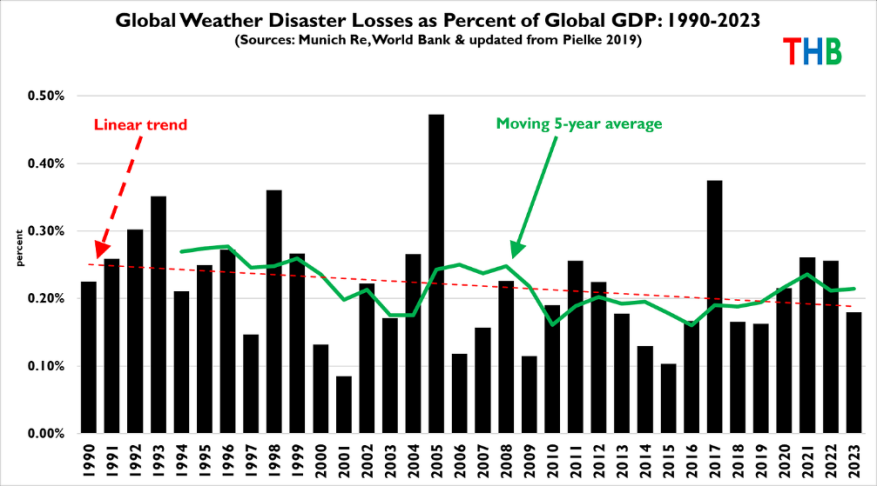
\includegraphics[width=0.9\textwidth]{bilder/bilderKlima-0082.png}\\[1cm]
\end{center}
\caption{Globale Wetterverluste als Anteil des BIP. Quelle: Pielke Jr. (2023)}
\end{figure}

Die Mainstream-Ökonomie-Position zur Klimapolitik-Frage wird am besten durch die Befunde der letzten drei Jahrzehnte aus Integrierten Bewertungsmodellen (IAMs) der Klimawandelpolitik repräsentiert, für die der Yale-Ökonom William Nordhaus 2018 den Nobelgedächtnispreis für Wirtschaftswissenschaften erhielt. IAMs kombinieren wirtschaftliche, klimatische und soziale Daten in einem einheitlichen Rahmen zur Simulation von Klimaschäden und Bewertung der optimalen Politikreaktion (Resources for the Future, 2025). Nordhaus' Arbeit hat allgemein bescheidene globale Klimapolitik unterstützt, mit aggressiven Maßnahmen, die größtenteils bis später im Jahrhundert aufgeschoben wurden.

Nordhaus entwickelte das sogenannte Dynamic Integrated Model of the Climate and Economy Modell, oder DICE, in den frühen 1990er Jahren (Nordhaus, 1993), um die Interaktion zwischen Klimawandel, Klimapolitik und globalem Wirtschaftswachstum über lange Zeiten zu studieren. DICE nimmt an, dass globale Emissionskontrolle kostenlos koordiniert werden kann und fragt, was das optimale Politikziel sein sollte. Die Klimakomponente des DICE-Modells basiert auf vereinfachter klimatologischer Modellierung. Die Version von DICE zur Zeit von Nordhaus' Nobelpreis-Verleihung wurde in Nordhaus (2018) beschrieben; sie hatte einen Klimasensitivitätsparameter von \SI{3.1}{\celsius} für CO$_2$-Verdopplung, konsistent mit der besten Schätzung in IPCC-Berichten (\SI{3.0}{\celsius}).

Das Baseline (Keine Politik) Szenario verursacht nur 0.4B\$ globale Minderungskosten und führt zu 134.2B\$ (Billionen Dollar) globalen Klimaschäden für Gesamtkosten von 134.6B\$. Die Klimamodellkomponente von DICE projiziert \SI{4.1}{\celsius} Erwärmung bis 2100 relativ zu vorindustriellen Temperaturen. Beachten Sie, dass dies eine höhere Schätzung der Erwärmung ist als viele IPCC-Klimamodelle.

Das Optimale Politik-Szenario weicht kaum vom Business-as-usual-Pfad ab. Es zielt auf \SI{+3.5}{\celsius} Erwärmung ab, mit anderen Worten, wir drosseln bescheiden die Nutzung fossiler Brennstoffe und leben ansonsten einfach mit fast der gesamten Erwärmung. Dies legt nahe, dass die meisten CO$_2$-Emissionen weniger schädlich sind als die Politiken, die notwendig wären, um sie zu mindern. Der Versuch, Erwärmung zu verhindern, führt dazu, dass Kosten schnell den Nutzen übersteigen. Das Verfolgen eines Ziels der Begrenzung der Erwärmung auf \SI{2.5}{\celsius} schafft Gesamtkosten von 177.8B\$,was 43.2B\$ schlechter ist als überhaupt nichts zu tun. Nordhaus bewertete nicht den Versuch, ein Paris-artiges Ziel von \SI{1.5}{\celsius} Erwärmung zu erreichen, aber es wäre noch kostspieliger.

Eine nachfolgende Ausgabe von DICE schließt höhere angenommene Schäden durch Erwärmung ein, was nicht überraschend zu aggressiveren Politikempfehlungen führt, wie im unten stehenden Abschnitt über die Sozialen Kosten von Kohlenstoff erklärt.


\subsection{Empirische Analyse von Klimawandel und Wirtschaftswachstum}
Viele andere Studien haben ökonometrische Methoden angewandt auf historische Daten, anstatt IAMs, um die potentielle Auswirkung des Klimawandels auf Wirtschaftswachstum zu studieren. Dell et al. (2012, hierin DJO12) war eine einflussreiche Studie, die ein Multi-Land-Panel von Daten auf nationaler Ebene verwendete, das von 1950 bis 2005 reichte, in dem sie Klima- und Wirtschaftsdaten durch Mitteln der Temperatur von der lokalen Gitterzellen-Ebene bis zur nationalen Ebene unter Verwendung von Bevölkerungsgewichtungen verknüpften. Sie fanden, dass Erwärmung einen unbedeutenden positiven Effekt auf Einkommenswachstum in reichen Ländern ergibt, aber einen signifikanten negativen Effekt in armen Ländern. Moore und Diaz (2015) modifizierten das DICE-Modell, um diesen Befund zu berücksichtigen und schlossen daraus, dass dies eine dramatisch höhere Soziale Kosten von Kohlenstoff implizierte aufgrund der sich verstärkenden Effekte von Einkommensverlusten über die Zeit.

Eine große nachfolgende Literatur hat die Robustheit der DJO12-Befunde debattiert. Burke et al. (2015) analysierten ein globales Panel mit Temperaturen, die bis zur nationalen Ebene gemittelt wurden und fanden einen negativen Effekt auf Wachstum durch Erwärmung in reichen und armen Ländern gleichermaßen, wenn die nationale Durchschnittstemperatur über \SI{13}{\celsius} liegt. Zhao et al. (2018) verwendeten den G-Econ-Datensatz von Nordhaus (2006), der wirtschaftliche Aktivität bis zur Gitterzellen-Ebene aufschlüsselt, replizierten DJO12-artige Ergebnisse auf derselben Teilmenge von Ländern, wie sie in DJO12 verwendet wurde, zeigten dann aber, dass auf der vollständigen globalen Stichprobe Erwärmung das Wachstum in reichen Ländern und armen Ländern gleichermaßen steigert, obwohl der positive Effekt in der letzteren Gruppe auf Gebiete beschränkt ist, wo lokale Temperaturen unter etwa \SI{16}{\celsius} liegen.
Greßer et al. (2021) entwickelten einen regionalen Wirtschaftsdatensatz für 1.542 subnationale Regionen rund um die Welt zwischen 2005 und 2015 und fanden, dass Temperatur keinen Effekt auf Wachstum hatte. Yang et al. (2023) aktualisierten den DJO12-Datensatz und wendeten einen Schätzer an, der robust gegen gemischte Stichprobenfrequenzen ist, und fanden, dass während Temperaturschocks einen temporären Effekt auf Einkommensniveaus ausübten, sie keinen signifikanten dauerhaften Effekt auf Wachstumsraten hatten.

Newell et al. (2021) bemerkten, dass es keine zugrundeliegende Theorie gibt, um ökonometrische Modellspezifikation in dieser Literatur zu leiten. Unter Berücksichtigung der willkürlichen Entscheidungen, welche erklärenden Variablen einzuschließen sind, identifizierten sie über 800 mögliche Modellspezifikationen. Unter Verwendung der Burke et al. (2015) Daten verwendeten sie eine Schätzmethode, die Modellunsicherheit berücksichtigt und fanden, dass die Modellform, die von Burke et al. (2015) bevorzugt wurde, welche negative Effekte der Erwärmung auf Wachstum sogar in reichen Ländern implizierte, explizit durch den optimalen Modellauswahlalgorithmus ausgeschlossen wird. Insgesamt konnten sie keinen Temperatureffekt auf BIP oder BIP-Wachstum entdecken, und sie schätzten das 95-Prozent-Konfidenzintervall für die Auswirkung auf globales Wachstum bis 2100 selbst unter dem übertriebenen RCP8.5--Erwärmungsszenario reicht von -86 Prozent bis +388 Prozent. Mit anderen Worten ist der Nettoeffekt wahrscheinlich positiv, aber zu unsicher, um von Null unterschieden zu werden.

Barker (2023) kritisierte die DJO12-Annahme, dass Länder in feste \emph{arme} und \emph{reiche} Kategorien gruppiert werden können basierend auf ihren Einkommen vor vielen Jahrzehnten. Er bemerkte, dass viele Länder einst arm waren, aber über die Zeit reich wurden, und wenn dies berücksichtigt wird, wurden die ursprünglichen Temperatureffekte, die von Dell et al. berichtet wurden, klein und unbedeutend.

Berg et al. (2023) argumentierten, dass Länder nicht in große Reich/Arm-Kategorien gruppiert werden sollten, weil sie zu heterogen sind. Sie schätzten stattdessen länderspezifische Temperaturreaktionskoeffizienten und gruppierten dann Länder mit ähnlichen Reaktionskoeffizienten in kleine Panels. Sie schätzten separat Reaktionen auf globale und idiosynkratische lokale Temperaturschocks, um das Klimasignal in Wetterdaten besser zu identifizieren. Insgesamt fanden sie, dass Länder, die negative Effekte der Erwärmung auf Wachstum erfahren, jene überzahlten, die positive Effekte erfahren, aber nur temporär: schließlich kehren sich die Effekte um, sodass etwa doppelt so viele Länder einen netto-positiven Wachstumseffekt erfahren. Sie fanden auch, dass globale (im Gegensatz zu lokalen) Temperaturveränderungen viel wahrscheinlicher dem Wachstum in armen Ländern als in reichen zugutekommen.
In einer Simulation bis 2100, sogar unter Verwendung des extremen RCP8.5-Szenarios, berechneten sie, dass der durchschnittliche globale BIP-Verlust nur 1,9 Prozent betragen würde verglichen mit einem Szenario ohne Erwärmung. Das heißt, anstatt dass die Wirtschaft um 400 Prozent wächst, würde sie um 392 Prozent wachsen. Die Implikation von Nordhaus' früherer Analyse ist, dass der Versuch, die Erwärmung zu verhindern, zu weit weniger als 392 Prozent Wachstum führen würde.

Zusammenfassend betrachten Ökonomen Klima als einen relativ unwichtigen Faktor im Wirtschaftswachstum, eine Ansicht, die vom IPCC selbst im Fünften Bewertungsbericht geteilt wird. Mainstream-Klimaökonomie hat anerkannt, dass CO$_2$-induzierte Erwärmung einige negative wirtschaftliche Effekte haben könnte, aber sie sind zu klein, um aggressive Minderungspolitik zu rechtfertigen, und der Versuch, globale Erwärmung zu "stoppen" oder zu begrenzen, selbst auf Niveaus weit über dem Pariser Ziel, wäre schlimmer als nichts zu tun. Eine einflussreiche Studie von 2012 legte nahe, dass globale Erwärmung dem Wachstum in armen Ländern schaden würde, aber der Befund hat sich anschließend als nicht robust erwiesen (Tol 2024). Studien, die Modellierungsunsicherheiten vollständig berücksichtigen, finden entweder keine Belege für einen negativen Effekt auf globales Wachstum durch CO$_2$-Emissionen oder finden arme Länder ebenso wahrscheinlich davon profitierend wie reiche Länder.

\begin{figure}[H]
\begin{center}
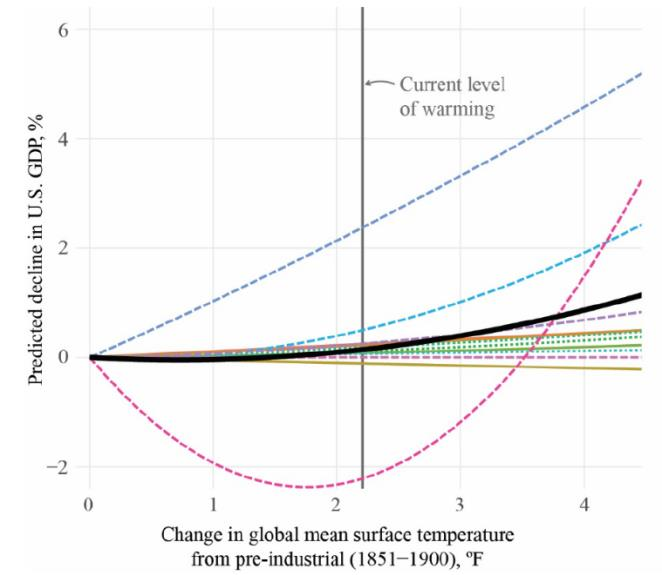
\includegraphics[width=0.8\textwidth]{bilder/bilderKlima-0084.jpg}\\[1cm]
\end{center}
\caption{Rückgang des US-BIP pro Grad Erwärmung. Quelle: CEA-OMB (2023)}
\end{figure}

Die Erwartung, dass signifikante globale Erwärmung eine kleine Auswirkung auf die US-Wirtschaft haben würde, wurde stillschweigend von der Biden-Administration anerkannt, selbst als der Präsident einen Klimanotstand ausrief. Abbildung 11.2, aus einem 2023 CEA-OMB-Bericht, zeigt das erwartete Dekrement im US-BIP als Funktion des Temperaturanstiegs. Die farbigen Linien zeigen die Ergebnisse von einem Dutzend peer-reviewter veröffentlichter Studien, während die durchgezogene schwarze Linie ihr Durchschnitt ist. Die Abbildung könnte zusammengefasst werden als "einige Prozent Auswirkung für einige Grad Erwärmung". Gegeben, dass die jährliche Wachstumsrate der Wirtschaft erwartungsgemäß 1-2 Prozent beträgt, ist die Auswirkung eines sich erwärmenden Globus auf das US-BIP tatsächlich vernachlässigbar.


\section{Modelle der sozialen Kosten von Kohlenstoff}
Die sozialen Kosten von Kohlenstoff (SCC) sind ein Instrument zur Quantifizierung der wirtschaftlichen Auswirkungen von Kohlendioxidemissionen und helfen politischen Entscheidungsträgern, die Kosten und Nutzen von Klimapolitiken abzuwägen. Sie schätzen den Schaden, der durch die Emission einer zusätzlichen Tonne CO$_2$ verursacht wird, ausgedrückt in Dollar. Formeller ausgedrückt sind die SCC der diskontierte Gegenwartswert des aktuellen und zukünftigen marginalen Verlusts der wirtschaftlichen Wohlfahrt aufgrund einer zusätzlichen Tonne CO$_2$, die in die Atmosphäre gelangt.

\subsection{Schätzung der SCC}
Obwohl die Literatur von \emph{Schätzungen} der SCC spricht, werden sie nicht auf die Art geschätzt, wie andere wirtschaftliche Statistiken geschätzt werden. Zum Beispiel können Daten über Markttransaktionen einschließlich Preise und Mengen verwendet werden, um die aktuelle Inflationsrate oder die Wachstumsrate des realen Pro-Kopf-Bruttoinlandsprodukts zu schätzen, und es gibt gut verstandene Ungewissheiten, die mit diesen Größen verbunden sind. Aber es sind keine Marktdaten verfügbar, um viele, wenn nicht die meisten der marginalen Schäden oder Vorteile zu messen, von denen angenommen wird, dass sie mit CO$_2$-Emissionen verbunden sind, sodass diese mit Hilfe von Wirtschaftsmodellen zugerechnet werden müssen.

Zum Beispiel ist eine einflussreiche Komponente einiger SCC-Berechnungen die wahrgenommenen sozialen Kosten, die mit einem veränderten Risiko zukünftiger Sterblichkeit aufgrund extremer Wetterereignisse verbunden sind. Es gibt keinen Markt, in dem Menschen einem solchen Risiko direkt einen Preis zuordnen können. Bestenfalls können Ökonomen versuchen, solche Werte abzuleiten, indem sie Transaktionen in verwandten Märkten wie Immobilien oder Versicherungen betrachten, aber die Isolierung der Komponente von Preisänderungen, die atmosphärischen CO$_2$-Konzentrationen zuzuschreiben sind, ist sehr schwierig.

Ökonomen verwenden IAMs (Integrated Assessment Models), um die SCC zu berechnen. Zwei der bekanntesten sind das Climate Framework for Uncertainty, Negotiation and Distribution (\emph{FUND}, Tol 1997) und Nordhaus' DICE. Die EPA (2023) führte neue für ihre jüngste Arbeit ein. IAMs enthalten eine \emph{Schadensfunktion} oder einen Satz von Funktionen, die die Umgebungstemperatur mit lokalen wirtschaftlichen Bedingungen verknüpfen. Die in der Schadensfunktion eingebetteten Annahmen werden die resultierende SCC weitgehend bestimmen. IAMs nehmen auch einen langfristigen Diskontsatz an oder, wie bei DICE, berechnen den optimalen internen Diskontsatz als Teil der Lösung.

Ein Ansatz zur Entwicklung einer Schadensfunktion besteht darin, mit Schätzungen der Kosten (oder Vorteile) der Erwärmung in spezifischen Sektoren in Ländern auf der ganzen Welt zu beginnen und zu einem globalen Betrag zu aggregieren. Dies war der Ansatz, der in FUND verwendet wurde. Ein alternativer Ansatz besteht darin, eine einfache Gleichung zu entwickeln, die das globale Einkommen gemäß einer einfachen quadratischen Funktion der durchschnittlichen globalen Temperatur bestraft. Dieser Ansatz wurde in DICE verwendet. Im Fall des FUND-Modells mussten viele hundert Parameter ausgewählt werden, während bei DICE nur drei benötigt wurden und ursprünglich gewählt wurden, um eine vorbestimmte Strafe (1.2\%) der globalen Leistung bei \SI{3}{\celsius} Erwärmung zuzuweisen, mit einem quadratischen Term, der impliziert, dass Schäden mit dem Quadrat der globalen durchschnittlichen Temperaturanomalie wachsen. Barrage und Nordhaus (2024) änderten kürzlich die Parameter, um die Strafe bei \SI{3}{\celsius} auf 1.6\% zu erhöhen, und fügten eine diskrete zusätzliche 1.0 Prozent BIP-Strafe bei \SI{3}{\celsius} Erwärmung hinzu, um \emph{Kipppunkte} (diskrete großmaßstäbliche Umweltveränderungen, die durch Überschreitung einer Erwärmungsschwelle ausgelöst werden) zu berücksichtigen, und eine \emph{beurteilende Anpassung} von 0,5 Prozent für ausgeschlossene Auswirkungen bei \SI{3}{\celsius} Erwärmung. Nicht überraschend generiert die neuere Version von DICE viel höhere SCC-Schätzungen als zuvor.

Die Konzepte der Schätzung und Ungewissheit lassen sich nicht ohne weiteres auf SCC-Berechnungen anwenden. Keine Menge der Datensammlung kann die Tatsache ändern, dass viele Komponenten der SCC unbekannt sind und auf Beurteilung und Meinung basierend auf dem Wissen der zugrundeliegenden Literatur über die physikalischen Auswirkungen des Klimawandels beruhen. SCC-Berechnungen werden daher am besten als "Wenn-dann"-Aussagen betrachtet: wenn die folgenden Annahmen gelten, dann ist die SCC \$X pro Tonne. Die Liste der "Wenn"--Aussagen umfasst die Prämisse, dass das Klima und die Wirtschaft der Welt entsprechend der Darstellung im IAM funktionieren. Eine Art, wie dies möglicherweise nicht zutrifft, liegt im Timing der Erwärmung. Jedes IAM nimmt einen Wert der Gleichgewichts--Klimasensitivität (ECS) an, der die Menge der Erwärmung kontrolliert, die aus CO$_2$--Emissionen resultiert, und kann frei variiert werden, um eine Verteilung von SCC--Werten zu generieren, die mit Ungewissheiten über die ECS verbunden sind. Aber wie Roe und Baumann (2013) darauf hinwiesen, steigt die Zeit bis zum Gleichgewicht mit dem Quadrat der ECS, sodass eine Aufwärtsanpassung des ECS--Parameters ohne eine angemessene Verlangsamung des Anpassungsprozesses verzerrte Gegenwartswert--Schadeneschätzungen ergeben kann. Insbesondere ist der obere Schwanz der Erwärmung, der mit einigen häufig verwendeten ECS--Verteilungen verbunden ist, physikalisch unmöglich für sogar tausend Jahre in die Zukunft (Roe und Baumann 2013), würde aber in einem IAM innerhalb weniger Jahrhunderte realisiert werden. Das Versäumnis, ECS mit der Zeit zum Gleichgewicht in Einklang zu bringen, wird zu einer Überschätzung des SCC--Werts führen.

\subsection{Variationen in den SCC}
Jede Ebene der IAM-Berechnung umfasst Annahmen, von denen einige einflussreicher sind als andere. Die wichtigsten Annahmen umfassen folgende:

\begin{itemize}
\item Der Diskontsatz: Klimaschäden fallen über einen langen Zeithorizont an, und Kosten ein oder zwei Jahrhunderte in der Zukunft müssen auf die Gegenwart diskontiert werden. Je höher der Diskontsatz, desto kleiner ist der Gegenwartswert zukünftiger Schäden und umgekehrt. Der Diskontsatz repräsentiert die Opportunitätskosten, heute Geld auszugeben, anstatt es zu investieren und dann morgen mehr zum Ausgeben zu haben. Einige Ökonomen haben für die Verwendung sehr niedriger Diskontsätze in SCC-Berechnungen argumentiert, was zu politischen Empfehlungen führt, die relativ große sofortige Investitionen in CO$_2$-Emissionsreduktionen befürworten. Der Nachteil ist, dass andere Investitionen potenziell eine größere Rendite für die Gesellschaft erzielen könnten.

\item Gleichgewichts-Klimasensitivität: IAMs haben üblicherweise einen Wert von \SI{3.0}{\celsius} oder \SI{3.1}{\celsius} entsprechend der IPCC-Leitlinien verwendet. Die neuesten datenbasierten ECS-Werte neigen dazu, niedriger als diese zu sein (siehe Kapitel 4). Dayaratna et al. (2017, 2020, 2023) haben gezeigt, dass die Verwendung niedrigerer empirisch abgeleiteter ECS-Werte die resultierende SCC-Schätzung dramatisch senkt, selbst wenn niedrige Diskontsätze verwendet werden.

\item Schadensfunktionskoeffizienten: IAMs nehmen an, dass CO$_2$ und Erwärmung Nettischäden verursachen, die exponentiell mit der Temperatur zunehmen. Jüngst haben IAMs auch Effekte aus angenommenen potenziellen Klima-Kipppunkten einbezogen. Das FUND-Modell berücksichtigte begrenzt, aber explizit CO$_2$-Düngungseffekte in der Landwirtschaft. Da die Koeffizienten vor der Veröffentlichung der aktuellen Belege für globale Ergrünung und das Ausmaß der Vorteile für Feldfrüchte durch erhöhtes CO$_2$ (siehe Kapitel 2 und 9) ausgewählt wurden, sind die Wachstumseffekte wahrscheinlich unterbewertet. Das DICE-Modell (und andere) schlossen keinen expliziten CO$_2$-Düngungsvorteil ein, außer in dem Umfang, in dem er in der Literatur berücksichtigt wurde, die bei der Auswahl der Schadensfunktionskoeffizienten konsultiert wurde. Die Schadensfunktion in FUND enthält einen Bereich, in dem geringe Erwärmung Nettovorteile in vielen Regionen erbringt, ein Befund, der durch ökonometrische Modelle der Erwärmung und des Wachstums (Berg et al. 2023) und ökonometrische Simulationen landwirtschaftlicher Veränderungen (McKitrick 2025) unterstützt wird. Die DICE-Schadensfunktion schließt konstruktionsbedingt Nettovorteile bei jedem Erwärmungsniveau aus.

\item Emissionsszenarien: IAMs generieren SCC-Schätzungen, die zunehmen, wenn die bereits bestehende CO$_2$-Konzentration steigt. Folglich wird der Wert der Schäden später im Jahrhundert höher sein, abhängig von den angenommenen Baseline-Emissionen in den kommenden Jahrzehnten.
\end{itemize}

Einige IAMs (wie DICE) schließen die Kosten für die Wirtschaft der Reduktion von CO$_2$-Emissionen ein, um die SCC entlang eines optimalen Wachstumspfads zu identifizieren. Wenn angenommen wird, dass CO$_2$-Emissionsreduktionen kostengünstig sind, dann wird das Modell zu dem Schluss kommen, dass die optimale Politik auf tiefere Emissionskürzungen abzielen sollte und umgekehrt.

Es ist aufschlussreich festzustellen, ob SCC-Ergebnisse invariant gegenüber Änderungen einiger Annahmen sind. Aber wenn verschiedene Annahmen zu höheren oder niedrigeren SCC-Werten führen, liefert die Änderung des SCC-Werts keinen prima facie Beweis für die Gültigkeit der Annahmen. Zum Beispiel erhöhte die U.S. Environmental Protection Agency 2023 ihren bevorzugten SCC-Wert um etwa das 5-fache gegenüber den Schätzungen, die sie zehn Jahre früher ausgegeben hatte. Dies geschah nicht, weil neue Daten gesammelt oder bessere mathematische Methoden erfunden worden waren, sondern weil neue Annahmen verwendet wurden, und die Gültigkeit dieser Annahmen war eine separate Frage. Tabulierungen auf EPA (2023) S. 81 zeigen, dass wenn ähnliche Annahmen wie in früheren Analysen angewendet worden wären, die Ergebnisse sich nicht wesentlich von zuvor unterschieden hätten. Eine neue Annahme war, dass globale landwirtschaftliche Schäden weit höher waren als zuvor angenommen, basierend auf einer Analyse in Moore et al. (2017). Aber wie in Kapitel 9 diskutiert, zeigte McKitrick (2025), dass Moore et al. (2017) eine Datenbank verwendet hatten, in der die Hälfte der CO$_2$-Veränderungsbeobachtungen fehlten. Als so viele dieser Beobachtungen wie möglich aus zugrundeliegenden Quellen wiederhergestellt und die Analyse erneut durchgeführt wurde, verschwanden die projizierten Ernteverluste und verwandelten sich in Gewinne bei allen Erwärmungsniveaus. Daher war der Teil der EPA-SCC-Revision, der auf landwirtschaftliche Ertragsverluste zurückzuführen war, ungerechtfertigt.

\subsection{Belege für niedrige SCC}
Kapitel 2 überprüfte Belege zu Klimawandel und Ergrünung, und Kapitel 9 betrachtete Klimawandel und U.S.-Landwirtschaft. Belege zeigen, dass CO$_2$-Düngung eine stärkere positive Wirkung auf die Landwirtschaft hat, als zu der Zeit bekannt war, als IAMs wie DICE und FUND parametrisiert wurden. Haverd et al. (2020) fanden, dass die beobachtete CO$_2$-Düngungsrate fast doppelt so hoch war wie von Pflanzenmodellen vorhergesagt.
Dayaratna et al. (2023) verwendeten die aktualisierte empirische ECS-Verteilungsschätzung von Lewis (2022), die moderne instrumentelle und paläoklimatische Temperaturaufzeichnungen assimiliert, und erlaubten einen 30-prozentigen Gewinn im CO$_2$-Düngungsvorteil im FUND-Modell, und fanden, dass selbst bei einem niedrigen Diskontsatz von 2.5 Prozent die mediane SCC ab 2050 nur 18.67 \$ beträgt, mit einer 24-prozentigen Wahrscheinlichkeit, dass der wahre Wert negativ ist. Bei einem fünfprozentigen Diskontsatz war der mediane SCC-Wert negativ bis Mitte der 2040er Jahre und betrug 2050 nur 0.37 \$ mit einer 49-prozentigen Wahrscheinlichkeit, negativ zu sein. Somit liefert unter vernünftigen Annahmen ein Mainstream-IAM, das aktualisierte wissenschaftliche Eingaben verwendet, Belege, die damit übereinstimmen, dass die SCC nicht signifikant größer als null ist.

Es sollte auch bemerkt werden, dass die SCC sich auf die sozialen Kosten von CO$_2$-Emissionen aus fossiler Brennstoffnutzung konzentriert. Sie ist nicht dazu bestimmt, die privaten marginalen Vorteile für Verbraucher und die Gesellschaft aus der Verfügbarkeit fossiler Brennstoffe zu messen. Die öffentliche Zahlungsbereitschaft für Brennstoffe aller Arten zeigt den Wert für die Gesellschaft von zuverlässiger, reichlicher fossiler Energie. Tol (2017) schätzt, dass der private Vorteil von Kohlenstoff groß ist im Verhältnis zu den sozialen Kosten. Dies kann veranschaulicht werden, indem man bemerkt, dass der Preis einer Gallone Benzin den marginalen Wert für den Verbraucher des Brennstoffs anzeigt. Nehmen wir an, wir nehmen relativ hohe soziale Kosten von Kohlenstoff von, sagen wir, 75 \$ pro Tonne an. Deflationiert durch einen MCPF\footnote{Grenzkosten öffentlicher Mittel(Marginal Cost of Public Funds): Der optimale CO$_2$-Steuersatz ergibt sich aus dem Quotienten von SCC und MCPF (Sandmo 1977).}-Wert von 1.5 würde das zu einer Kohlenstoffsteuer von 50 \$ pro Tonne führen, was etwa 44 Cent pro Gallone Benzin entspricht (Lavelle, 2019). Ein Vorsteuerpreis von 3.00 \$ pro Gallone würde implizieren, dass der marginale soziale Nutzen des Brennstoffs fast siebenmal die marginalen sozialen Kosten beträgt.

\subsection{Kipppunkte}
SCC-Berechnungen berücksichtigen typischerweise graduelle Auswirkungen eines sich erwärmenden Klimas, wie langsam schmelzende Gletscher und steigende Durchschnittstemperaturen. Ein Treiber potenziell hoher Werte der sozialen Kosten von Kohlenstoff (SCC) ist die Einführung diskreter katastrophaler Ergebnisse, die mit abrupten Veränderungen verbunden sind, in Modelle (Dietz et al., 2021). Sie werden oft als \emph{Kipppunkte} bezeichnet.

Der Begriff \emph{Kipppunkt} vermischt zwei verschiedene physikalische Konzepte, die unterschiedliche Forschungsherausforderungen darstellen. Viele physikalische Systeme sind von Natur aus stabil, es sei denn, sie werden mit ausreichender externer Energie beeinflusst. Zum Beispiel kann eine Eiskappe über einen weiten Temperaturbereich intakt bleiben, aber sobald die Temperatur die \SI{0}{\celsius}-Schwelle überschreitet, schmilzt sie. Solche Diskontinuitäten sind in der Natur allgegenwärtig und erfordern eine externe Kraft. Ob die Kraft groß sein muss im Verhältnis zur Größe des Systems, hängt von der zugrundeliegenden Stabilität des Systems ab.

Ein anderer Typ von Kipppunkt wird Bifurkation genannt und entsteht aus dem Studium der internen Dynamik nichtlinearer Systeme (Crawford, 1991). Es wurde beobachtet, dass viele Systeme mehr als einen Gleichgewichtspunkt haben und zwischen ihnen mit minimalem oder ohne externen Einfluss wechseln können. Zum Beispiel könnte ein Wettersystem zwei verschiedene Gleichgewichtszustände haben: einen ruhigen und einen mit einem Tornado. Ein Übergang von einem zum anderen kann entweder ohne externe Kraft oder mit einer winzigen Veränderung geschehen, wie dem Flügelschlag des sprichwörtlichen Schmetterlings (Shen et al. 2014). Der Begriff "Kipppunkt" wird manchmal verwendet, um eine Bifurkation dieses Typs zu bezeichnen und impliziert eine dem System selbst innewohnende Instabilität, die nicht notwendigerweise von äußeren Kräften abhängt. Sie hängt stattdessen von Parametern des Systems ab, die Werte annehmen, die das Entstehen von Bifurkationen unterstützen (Crawford, 1991).

Die zwei verschiedenen Konzepte implizieren unterschiedliche Forschungsfragen. Bezüglich des ersten interessieren wir uns dafür, ob Komponenten des Klimasystems anfällig für abrupte Diskontinuitäten als Reaktion auf ausreichend große anthropogene Antriebe sind. Bezüglich des zweiten interessieren wir uns dafür, ob das Klimasystem der Erde inhärente Bifurkationen hat, die die Möglichkeit abrupter Übergänge mit oder ohne externe Antriebe implizieren.

Modelle wurden entwickelt, die implizieren, dass der zweite Typ eine Möglichkeit ist. Kypke et al. (2020) präsentierten ein einfaches Klimamodell, in dem die THG-Konzentration einer der Parameter ist, die das Entstehen von Bifurkationen des arktischen Klimas zu einem mit sowohl kalten als auch warmen Gleichgewichten kontrolliert. Wenn ausreichend hoher THG-Antrieb kombiniert mit einer ausreichend hohen Rate des ozeanischen Wärmetransports auferlegt wird, wird eine Bifurkation möglich. Allgemeiner wurde beobachtet, dass GCMs Bifurkationen und multiple Gleichgewichte enthalten (Brunetti und Ragon, 2023).

Die mögliche Existenz von Bifurkationen im Klimasystem der Erde impliziert, dass abrupte Übergänge möglich sind, nicht nur als Reaktion auf große Antriebe, sondern auch auf kleine Störungen. Dies ordnet Kipppunkte in die Kategorie von Ereignissen mit geringer Wahrscheinlichkeit und potenziell katastrophalen Auswirkungen ein, wie große Meteoriteneinschläge. Eine wichtige Frage ist, ob solche Arten von Kipppunkten vorhergesagt werden können. Die aktuelle Forschung hat diese Frage nicht gelöst (Dakos et al., 2024) und könnte dies tatsächlich nicht können, da eine Implikation des \emph{Schmetterlingseffekts} die Existenz von Vorhersagbarkeitsgrenzen nichtlinearer Systeme ist (Palmer et al., 2014). Es ist daher nicht offensichtlich, wie solche Möglichkeiten in SCC-Berechnungen einbezogen werden können. Kleine Variationen in den Annahmen werden zu willkürlich großen Variationen in der resultierenden SCC führen, ohne Grundlage für eine Wahl zwischen ihnen. Wenn solche Kipppunkte möglich sind, ist die angemessenste Haltung für die Wirtschaftspolitik, die Widerstandsfähigkeit gegenüber jeder Form externer Katastrophe zu maximieren, da es unwahrscheinlich ist, dass wir sie vorhersagen oder ihr Auftreten verhindern könnten.

AR6 (WGI, Kapitel 1) konzentriert sich hauptsächlich auf den ersten Typ von Kipppunkt, nämlich eine abrupte Veränderung als Reaktion auf externe Antriebe. Dies ist auch die Bedeutung, die mit der populären Verwendung des \emph{Kipppunkt}-Konzepts in Diskussionen über den Klimawandel verbunden ist (siehe \url{https://report-2023.global-tipping-points.org/what-is-a-tipping-point/} zum Beispiel). Wie von AR6 zusammengefasst, gibt es Belege für abrupte Veränderungen in der Paläoklimaaufzeichnung, und einige dieser Ereignisse wurden als Kipppunkte interpretiert. Einige Projektionen mit Erdsystemmodellen haben zum Beispiel Kipppunkte wie das Absterben des Amazonas-Regenwaldes als Reaktion auf spezifizierte Werte der CO$_2$-Konzentration oder Temperaturanstiege produziert.

Der Alarm um Klima-Kipppunkte spiegelt sich in dem Global Tipping Points Report wider, der am 6. Dezember 2023 bei COP28 vorgestellt wurde (Lenton et al., 2023). Er identifiziert mehr als 25 Teile des Klimasystems, die als Kipppunkte bezeichnet werden. Was als Klima-"Kipppunkt" klassifiziert wird, ist ein bewegliches Ziel. Die häufigsten Beispiele in der Literatur und in Bewertungsberichten umfassen: Zerfall der grönländischen Eisdecke, Zerfall der westantarktischen Eisdecke, sommerliches Verschwinden des arktischen Meereises, Absterben des Amazonas-Regenwaldes, Korallenriff-Absterben, Auftauen von Permafrost und Methanhydraten, Kollaps der atlantischen meridionalen Umwälzzirkulation, Verschiebung borealer Wälder, Verschiebung des westafrikanischen Monsuns und Verschiebung des indischen Monsuns.

Alle solchen Kipppunkte erfordern ein gewisses Maß an Systeminstabilität, um einen abrupten Übergang als Reaktion auf die Erwärmung zu zeigen. Aus diesem Grund scheint es sehr wenig zu geben, um zwischen einem Kippereignis und natürlicher Klimavariabilität zu unterscheiden. Natürliche Klimavariabilität hat in der Vergangenheit Verschiebungen in den west-afrikanischen und indischen Monsunen, Amazonas-Wald- und Korallenriff-Absterben und Zerfall von Teilen der grönländischen und westantarktischen Eisschilde hervorgebracht. Diese Auswirkungen können sich auf den Dekaden- und Jahrhundertzeitskalen umkehren, die mit natürlicher Klimavariabilität und Ökosystemreaktionen verbunden sind.

Einige abrupte Veränderungen sind potenziell folgenreicher, einschließlich des Kollapses der westantarktischen Eisdecke und des Kollapses der atlantischen meridionalen Umwälzzirkulation (AMOC). AR6 WG1 Summary for Policy Makers stellt fest:

\begin{quote}
Die atlantische meridionale Umwälzzirkulation wird sich sehr wahrscheinlich über das 21. Jahrhundert für alle Emissionsszenarien abschwächen. Während es hohes Vertrauen in den Rückgang des 21. Jahrhunderts gibt, gibt es nur geringes Vertrauen in das Ausmaß des Trends. Es gibt mittleres Vertrauen, dass es vor 2100 keinen abrupten Kollaps geben wird. (C.3.4)
Es gibt begrenzte Belege für Ergebnisse mit geringer Wahrscheinlichkeit und hohen Auswirkungen (resultierend aus Eisschild-Instabilitätsprozessen, die durch tiefe Ungewissheit charakterisiert sind und in einigen Fällen Kipppunkte involvieren), die den Eisverlust vom antarktischen Eisschild für Jahrhunderte unter hohen THG-Emissionsszenarien stark erhöhen würden (z.B. SSP5-8.5). (B.5.2)
\end{quote}

Für SCC-Berechnungen ist die durch diese Art von Kipppunkt implizierte Forschungsfrage, ob solche Ereignisse in der Vergangenheit unter Klimabedingungen beobachtet wurden, die dem ähneln, was wir derzeit erleben oder in naher Zukunft erleben werden. AR6 findet wenig Belege für einen bevorstehenden Kollaps der atlantischen meridionalen Umwälzzirkulation oder der westantarktischen Eisdecke. Es stellt fest, dass es keinen Kipppunkt gibt, der mit arktischem Meereis verbunden ist (AR6 Technical Summary S. 76).

Dietz et al. bezogen mehrere potenzielle Kipppunkte (abrupte Veränderungen) in ein SCC-Modell ein und fanden, dass sie etwa 25 Prozent zur Schätzung hinzufügten, hauptsächlich verbunden mit auftauendem Permafrost und Freisetzung von Methanhydraten. Das IPCC betrachtet dieses Szenario jedoch als sehr unwahrscheinlich (AR6 Technical Summary S. 107).

Zusammenfassend könnte es unbekannte Bifurkations-Kipppunkte geben, die mit natürlichen Klimaprozessen verbunden sind, aber diese Möglichkeit übersetzt sich nicht in spezifische Leitlinien für die SCC. Es gibt potenzielle abrupte Veränderungspunkte im Klimasystem als Reaktion auf die Erwärmung, obwohl das IPCC den meisten, einschließlich der größten, geringe Wahrscheinlichkeiten zuweist. Wenn diese berücksichtigt wurden, ist das Ergebnis nur eine bescheidene Erhöhung des SCC-Werts im 21. Jahrhundert.

\subsection{Gibt es Alternativen?}
Es wird zunehmend argumentiert, dass die SCC zu variabel ist, um für politische Entscheidungsträger nützlich zu sein. Cambridge Econometrics (Thoung, 2017) erklärte, es sei \emph{Zeit, sie zu töten} aufgrund von Ungewissheiten. Das Vereinigte Königreich und die EU verwenden die SCC nicht mehr für Politikbewertungen und entscheiden sich für \emph{zielkonsistente} Kohlenstoffpreise (UK Department for Energy Security and Net Zero 2022, Dunne 2017). Die Ungewissheit von SCC-Schätzungen bedeutet jedoch nicht, dass andere regulatorische Instrumente von Natur aus besser oder effizienter sind. Viele Emissionsvorschriften (wie Elektrofahrzeug-Mandate, Erneuerbare-Energie-Mandate, Energieeffizienz-Vorschriften und Verbote bestimmter Arten von Haushaltsgeräten) kosten weit mehr pro Tonne Emissionsminderung als jede Mainstream-SCC-Schätzung, was ausreicht, um festzustellen, dass sie einen Kosten-Nutzen-Test nicht bestehen.

\vfill
\noindent\textbf{Literaturverzeichnis:}

\begingroup
\parindent=0pt
\everypar{\hangindent=2em\hangafter=1\relax}

AR6: Intergovernmental Panel on Climate Change Sixth Assessment Report (2021) Working Group I
Contribution. www.ipcc.ch.

Arent, D.J., R.S.J. Tol, E. Faust, J.P. Hella, S. Kumar, K.M. Strzepek, F.L. Tóth, and D. Yan (2014) Key
economic sectors and services. In: Climate Change 2014: Impacts, Adaptation, and Vulnerability. Part
A: Global and Sectoral Aspects. Contribution of Working Group II to the Fifth Assessment Report of
the Intergovernmental Panel on Climate Change [Field, C.B., V.R. Barros, D.J. Dokken, K.J. Mach,
M.D. Mastrandrea, T.E. Bilir, M. Chatterjee, K.L. Ebi, Y.O. Estrada, R.C. Genova, B. Girma, E.S.
Kissel, A.N. Levy, S. MacCracken, P.R. Mastrandrea, and L.L.White (eds.)]. Cambridge University
Press, Cambridge, United Kingdom and New York, NY, USA, pp. 659-
708.\url{https://www.ipcc.ch/site/assets/uploads/2018/02/WGIIAR5-Chap10_FINAL.pdf}

Barker, D. (2023) Temperature Shocks and Economic Growth: Comment on Dell, Jones, and Olken. Econ
Journal Watch 20(2) 234-253 \url{https://econjwatch.org/articles/temperature-shocks-and-economic-
growth-comment-on-dell-jones-and-olken}

Barrage, Lint and William Nordhaus (2024) Policies, projections, and the social cost of carbon: Results
from the DICE-2023 model. Proceedings of the National Academy of Sciences 121 (13) e2312030121
\url{https://doi.org/10.1073/pnas.2312030121}

Berg, Kimberly, Chadwick C Curtis and Nelson Mark. (2021) GDP and temperature: Evidence on cross-
country response heterogeneity. NBER Working Paper 31327 June 2023
\url{http://www.nber.org/papers/w31327}

Blickle, Kristian; Sarah N. Hamerling, and Donald P. Morgan (2021) : How bad are weather disasters for
banks?, Staff Reports, No. 990, Federal Reserve Bank of New York, New York, NY
\url{https://www.econstor.eu/bitstream/10419/247913/1/sr990.pdf}

Brunetti, Maura and Charline Ragon (2023) Attractors and bifurcation diagrams in complex climate models.
Physical Review E 107 054214 \url{https://journals.aps.org/pre/abstract/10.1103/PhysRevE.107.054214}

Burke, Marshall, Solomon M Hsiang, and Edward Miguel (2015). Global non-linear effect of temperature
on economic production. Nature, 527(7577):235–239.

Council of Economic Advisors-Office of Management and Budget (CEA-OMB 2023) Methodologies and
considerations for integrating the physical and transition risks of climate change into macroeconomic
forecasting for the president’s budget. March 13, 2023. \url{https://bidenwhitehouse.archives.gov/wp-
content/uploads/2023/03/CEA-OMB-White-Paper.pdf}

Crawford, John D (1991) Introduction to Bifurcation Theory. Reviews of Modern Physics 63(4) October
1991 991—1037.

Dakos, Vasilis, Chris Boulton, Joshua Buxton et al. (2024) Tipping point detection and early warnings in
climate, ecological, and human systems. Earth System Dynamics 15 1117—1135
\url{https://doi.org/10.5194/esd-15-1117-2024}

Dayaratna, Kevin and Ross McKitrick (2023) "Reply to comment on “climate sensitivity, agricultural
productivity and the social cost of carbon in fund” by Philip Meyer" Environmental Economics and
Policy Studies 2023 link.springer.com/article/10.1007/s10018-023-00364-2

Dayaratna, Kevin, Ross McKitrick and David Kreutzer (2017) Empirically-Constrained Climate Sensitivity
and the Social Cost of Carbon. Climate Change Economics April 2017 DOI:
\url{http://dx.doi.org/10.1142/S2010007817500063}

Dayaratna, Kevin, Ross McKitrick and Patrick J. Michaels (2020) Climate Sensitivity, Agricultural
Productivity and the Social Cost of Carbon in FUND. Environmental Economics and Policy Studies
\url{https://doi.org/10.1007/s10018-020-00263-w}

Dell, Melissa, Benjamin F. Jones, and Benjamin A. Olken (2012). Temperature shocks and economic
growth: Evidence from the last half century. American economic journal: Macroeconomics, 4(3):66–
95, 2012. ISSN 1945-7707.

Dietz, S., J. Rising, T. Stoerk, G. Wagner (2021) Economic impact of tipping points in the climate system.
Proceedings of the National Academy of Science 2021 Vol. 118 No. 34 e2103081118

Dunne, Daisy (2017), “Q\&A: The Social Cost of Carbon,” Carbon Brief, February 14, 2017,
\url{https://www.carbonbrief.org/qa-social-cost-carbon/}

Formetta, Giuseppe and Luc Feyen (2019) Empirical evidence of declining global vulnerability to
climate-related hazards. Global Environmental Change 57 101920
\url{https://doi.org/10.1016/j.gloenvcha.2019.05.004}

Greßer, Christina, Daniel Meierrieks, and David Stadelmann (2021) The link between regional temperature
and regional incomes: econometric evidence with sub-national data. Economic Policy, 36(107):523–
550, 2021.

Haverd, V., Raupach, M., Briggs, P., et al. (2020). Higher than expected CO$_2$ fertilization inferred from
leaf to global observations. Global Change Biology, 26, 2390–2402.

Hu, Bin and Ross McKitrick (2015) Climatic Variations and the Market Value of Insurance Firms.
Journal of Insurance Issues Vol. 39, No. 1, pp. 92-111 \url{https://www.jstor.org/stable/43741103}

Kypke, K. L., Langford, W. F., and Willms, A. R.: Anthropocene climate bifurcation, Nonlinear Processes
in Geophysics, 27, 391–409, \url{https://doi.org/10.5194/npg-27-391-2020}, 2020.

Lavelle, Marianne (2019) Carbon Tax Plans: How They Compare and Why Oil Giants Support One of
Them. Inside Climate News March 7, 2019 \url{https://insideclimatenews.org/news/07032019/carbon-tax-proposals-compare-baker-shultz-exxon-conocophillips-ccl-congress/}

Lenton, T.M., D.I. Armstrong McKay, et al. (eds) (2023) The Global Tipping Points Report 2023.
University of Exeter, Exeter, UK. \url{https://report-2023.global-tipping-points.org/}

Lewis, N., (2013) An objective Bayesian, improved approach for applying optimal fingerprint techniques
to estimate climate sensitivity. Journal of Climate, 26, 7414-7429.
\url{https://journals.ametsoc.org/doi/abs/10.1175/JCLI-D-12-00473.1}

McKitrick, Ross R. (2025) Extended Crop Yield Meta-analysis Data do not Support Upward SCC
Revision. Scientific Reports 15 article 5575 \url{https://www.nature.com/articles/s41598-025-90254-2}

Mohaddes, Kamiar, Ryan Ng., Hashem Psaran, Mehdi Raissi and Jui-Chung Yang (2023) Climate change
and economic activity: evidence from US states. Oxford Open Economics Vol 2 odac010
\url{https://doi.org/10.1093/ooec/odac010}

Moore, Frances C. and Delavane B. Diaz (2015) Temperature impacts on economic growth warrant
stringent mitigation policy. Nature Climate Change, 5(2):127–131, 2015. ISSN 1758-678X.
Moore FC, Baldos U, Hertel T, Diaz D (2017) New science of climate change impacts on agriculture
implies higher social cost of carbon. Nature Communications 8:1607. \url{https://doi.org/10.1038/s41467-017-01792-x}

Newell, Richard G., Brian C. Prest, and Steven E. Sexton (2021). The GDP-temperature relationship:
Implications for climate change damages. Journal of Environmental Economics and Management, 108
\url{https://doi.org/10.1016/j.jeem.2021.102445}

Nordhaus, William (2006). Geography and macroeconomics: New data and new findings. Proceedings of
the National Academy of Sciences, 103(10):3510–3517, 2006. ISSN 0027-8424.

Nordhaus, William. (2018) Projections and Uncertainties About Climate Change in an Era of Minimal
Climate Policies. American Economic Journal: Economic Policy August 2018, 10(3): 333-360.
\url{https://pubs.aeaweb.org/doi/pdfplus/10.1257/pol.20170046}

Nordhaus, W. (1993) Optimal Greenhouse-Gas Reductions and Tax Policy in the "DICE" Model
American Economic Review Vol. 83, No. 2, (Papers and Proceedings) pp.313-317.

O’Neill, Brian C. (2023) Envisioning a future with climate change. Nature Climate Change 13, pages 874–
876 \url{https://www.nature.com/articles/s41558-023-01784-4}

Palmer, TN, A Döring and G Seregin (2014) The real butterfly effect. Nonlinearity 27(9) 10.1088/0951-
7715/27/9/R123 \url{https://iopscience.iop.org/article/10.1088/0951-7715/27/9/R123/meta}

Pielke Jr., Roger (2018): Tracking progress on the economic costs of disasters under the indicators of the
sustainable development goals, Environmental Hazards, \url{DOI: 10.1080/17477891.2018.1540343}

Pielke Jr., Roger (2020) Economic ‘normalisation’ of disaster losses 1998–2020: a literature review and
assessment,” Environmental Hazards, 2020, pp. 1-19

Pielke Jr., Roger (2023) Global disaster losses: 1990-2023 Substack essay
\url{https://rogerpielkejr.substack.com/p/global-disaster-losses1990-2023}

Resources for the Future (2025) “Social Cost of Carbon Explorer,” Resources for the Future website,
accessed April 22, 2025, \url{https://www.rff.org/publications/data-tools/scc-explorer/}.

Roe, Gerard H. and Yoram Bauman (2013) Climate Sensitivity: Should the climate tail wag the policy
dog? Climatic Change (2013) 117:647–662 DOI 10.1007/s10584-012-0582-6

Sandmo, Agnar (1975) \emph{Optimal Taxation in the Presence of Externalities.} Swedish Journal of Economics
77 (1), 86–98.

Schelling, Thomas C (1992) Some economics of global warming. The American Economic Review, 82
(1):1–14.

Shen, Bo-Wen, Roger A Pielke Sr and Xubin Zeng (2023) The 50th Anniversary of the Metaphorical
Butterfly Effect since Lorenz (1972): Multistability, Multiscale Predictability, and Sensitivity in
Numerical Models. Atmosphere 2023 14(8) \url{https://doi.org/10.3390/atmos14081279}

Storm, S (2017) “How the Invisible Hand is Supposed to Adjust the Natural Thermostat: A Guide for the
Perplexed.” Science and Engineering Ethics vol 23: 1307—1331.

Thoung, Chris (2017) “Is It Time to Kill Off the Social Cost of Carbon?” Cambridge Econometrics Blog,
September 14, 2017, \url{https://www.camecon.com/blog/time-kill-social-cost-carbon/}.

Tol, Richard S.J. (1997) On the optimal control of carbon dioxide emissions: an application of FUND
Environmental Modeling and Assessment 2: 151—163.

Tol, Richard S.J. (2017). "The Private Benefit of Carbon and its Social Cost," Working Paper Series 0717, Department of Economics, University of Sussex Business School.
\url{https://ideas.repec.org/p/sus/susewp/0717.html}

Tol, Richard S.J. (2024) A meta-analysis of the total economic impact of climate change. Energy Policy
185 113922 \url{https://doi.org/10.1016/j.enpol.2023.113922}

UK Department for Energy Security and Net Zero (2022). “Carbon Valuation.” GOV.UK, last updated
April 4, 2022. \url{https://www.gov.uk/government/collections/carbon-valuation--2}.

US Environmental Protection Agency (2023) Supplementary Material for the Regulatory Impact Analysis
for the Final Rulemaking, “Standards of Performance for New, Reconstructed, and Modified Sources
and Emissions Guidelines for Existing Sources: Oil and Natural Gas Sector Climate Review”, EPA
Report on the Social Cost of Greenhouse Gases: Estimates Incorporating Recent Scientific Advances,
November 2023, \url{https://www.epa.gov/system/files/documents/2023-
12/epa_scghg_2023_report_final.pdf accessed February 28, 2024.}

Yang, Yimin, Fei Jia, and Haoran Li. Estimation of panel data models with mixed sampling frequencies
(2023). Oxford Bulletin of Economics and Statistics, 85(3):514–544.

Zhao, Xiaobing, Mason Gerety, and Nicolai V. Kuminoff (2018) Revisiting the temperature-economic
growth relationship using global subnational data. Journal of environmental management, 223:537–
544, 2018.

\endgroup

\cleardoublepage
%\numberwithin{figure}{chapter}
\chapter{GLOBALE KLIMAAUSWIRKUNGEN VON U.S.-EMISSIONSPOLITIKEN}

\paragraph{Kapitelzusammenfassung}
\begin{quote}
Von U.S.--Politikmaßnahmen wird erwartet, dass sie unentdeckbar kleine direkte Auswirkungen auf das globale Klima haben werden, und alle Effekte werden nur mit langen Verzögerungen auftreten.
\end{quote}
\section{Das Skalenproblem}
Die Emissionsraten und atmosphärischen Konzentrationen von Kriterien-Luftschadstoffen sind eng verbunden, weil ihre Lebensdauern kurz und ihre Konzentrationen klein sind; wenn lokale Emissionen reduziert werden, sinkt die lokale Verschmutzungskonzentration schnell, normalerweise innerhalb weniger Tage. Aber die globale durchschnittliche CO$_2$-Konzentration verhält sich sehr anders, da sich Emissionen global vermischen und der globale Kohlenstoffkreislauf umfangreich und langsam ist. Jede Änderung lokaler CO$_2$-Emissionen heute wird nur einen sehr kleinen globalen Effekt haben, und nur mit einer langen Verzögerung.
Nach der Emission eines Pulses (Freisetzung) von CO$_2$ in die Atmosphäre werden nur etwa 40 ± 15 Prozent des zusätzlichen CO$_2$ nach zwanzig Jahren sequestriert worden sein. Dieser Anteil steigt auf 75 ± 10 Prozent nach tausend Jahren, und der Rest wird über die folgenden Zehntausende von Jahren graduell entfernt werden (Ciais et al., 2013, S. 472-473). Folglich würde jede Reduktion der U.S.-Emissionen nur bescheiden verlangsamen, aber nicht verhindern, den Anstieg der globalen CO$_2$-Konzentration. Und selbst wenn globale Emissionen morgen stoppen würden, würde es Jahrzehnte oder Jahrhunderte dauern, eine bedeutsame Reduktion der globalen CO$_2$-Konzentration und damit menschlicher Einflüsse auf das Klima zu sehen.
Die Reduktion des atmosphärischen CO$_2$-Bestands würde erfordern, dass Emissionen unter die natürliche Sequestrierungsrate fallen, unter der Annahme, dass die gesamte Zunahme anthropogen ist. Da diese Rate in den letzten Jahrzehnten durchschnittlich etwa 50 Prozent der Emissionen betragen hat, würde eine Reduktion globaler Emissionen um 50 Prozent (zumindest vorübergehend) den Anstieg des atmosphärischen CO$_2$ stoppen. Das Kyoto-Protokoll von 1997 schlug vor, die CO$_2$-Emissionen der Industrienationen auf bescheidene fünf Prozent unter die Niveaus von 1990 bis zum Jahr 2012 zu begrenzen. Obwohl diese Politik für die meisten Nationen zu schwierig umzusetzen war, hätte vollständige Einhaltung die atmosphärischen CO$_2$-Niveaus nicht wesentlich reduziert. Sie hätte nur das CO$_2$-Wachstum leicht verlangsamt und das projizierte Niveau für das Jahr 2100 stattdessen in 2105 erreicht (Wigley, 1998). Lomborg (2016) schätzte, dass vollständige Einhaltung der ursprünglichen Verpflichtungen im Pariser Abkommen die Erwärmung nicht stoppen würde, sie würde nur etwa \SI{0.1}{\celsius} Erwärmung verhindern und das Erreichen der Baseline-Temperaturniveaus des Jahres 2100 um etwa ein Jahrzehnt verzögern.
Somit werden im Kontrast zur konventionellen Luftverschmutzungskontrolle selbst drastische lokale Maßnahmen vernachlässigbare lokale Effekte haben, und nur mit einer langen Verzögerung. Die Praxis, unilaterale U.S.-Reduktionen als "Bekämpfung des Klimawandels" oder "Maßnahmen zum Klima" zu bezeichnen, unter der Annahme, dass wir den Klimawandel stoppen können, spiegelt daher ein profundes Missverständnis des Ausmaßes des Problems wider.

\section{Fallstudie: U.S.-Kraftfahrzeugemissionen}
Das Skalenproblem kann mit Bezug auf U.S.-Kraftfahrzeuge veranschaulicht werden. Die EPA-Gefährdungsfeststellung von 2009 konzentrierte sich auf CO$_2$-Emissionen von Pkw und leichten Lastkraftwagen in den U.S., weil Abschnitt 202(a) des Clean Air Act die EPA verpflichtet, Emissionsstandards für Kraftfahrzeuge festzulegen, wenn festgestellt wird, dass Schadstoffe die öffentliche Gesundheit oder das Wohlergehen gefährden. Die Gefährdungsfeststellung von 2009 verpflichtete daher die EPA, Emissionen neuer Kraftfahrzeuge zu regulieren, angeblich um klimabezogene Schäden für die U.S.-Öffentlichkeit zu reduzieren oder zu eliminieren.
Zwei Fragen, die sich natürlich stellen, sind: (1) Wie groß wäre eine Reduktion der CO$_2$-Emissionen, die aus einer solchen Regulierung resultieren würde? und (2) Was wären die Klimaauswirkungen einer solchen Regulierung?
Die erste Frage kann beantwortet werden, indem U.S.-fahrzeugbasierte CO$_2$-Emissionen mit dem globalen Total verglichen werden. Die zweite Frage kann beantwortet werden, indem die Tatsache verwendet wird, dass die Reduktion der globalen Erwärmung, entsprechend den Modellen, auf die sich die EPA stützt, proportional zur Reduktion globaler Emissionen wäre, unter Berücksichtigung der Tatsache, dass die Änderung im CO$_2$-Gehalt der Atmosphäre in einem gegebenen Jahr das Resultat der gesamten globalen CO$_2$-Emissionen ist, nicht nur der U.S.-Emissionen.
Im Jahr 2022 beliefen sich die Emissionen von U.S.-Pkw und leichten Lastkraftwagen auf insgesamt 1,05 Milliarden Tonnen Kohlendioxid (GtCO$_2$, EPA 2024). Währenddessen beliefen sich die globalen CO$_2$-Emissionen aus Energienutzung auf insgesamt 34,6 GtCO$_2$ (Energy Institute 2024). Daher machen U.S.-Pkw und leichte Lastkraftwagen nur 3,0 Prozent der globalen energiebezogenen CO$_2$-Emissionen aus. Als erste Näherung können wir sagen, dass selbst die Eliminierung aller U.S.-fahrzeugbasierten Emissionen die Akkumulation von CO$_2$ in der Atmosphäre über ein Jahrhundert um ein Jahr oder zwei verzögern würde.
Es würde auch den gesamten Erwärmungstrend um höchstens etwa 3 Prozent reduzieren. Für den Zeitraum 1979-2023, der die umfangreichste globale Abdeckung verschiedener Wetterdatentypen hat, werden Erwärmungstrends mit einer Präzision von etwa ± 15 Prozent bestimmt, sodass die Auswirkung der Reduktion der globalen Erwärmungsrate durch Eliminierung der U.S.-Fahrzeug-CO$_2$-Emissionen weit unterhalb der Messbarkeitsgrenze läge. Angesichts dessen, dass die global-durch\-schnittliche Temperatur die direkteste Klimawandel-Metrik ist, wären Auswirkungen auf sekundäre Klimametriken (z.B. schweres Wetter, Überschwemmungen, Dürre, etc.) durch Reduktion der U.S.-Fahrzeug-CO$_2$-Emissionen noch weniger messbar.
Folglich können im Gegensatz zum Fall lokaler Luftschadstoffe wie Partikel und Ozon selbst die aggressivsten regulatorischen Maßnahmen zu Treibhausgasemissionen von U.S.-Fahrzeugen nicht erwartet werden, angebliche Klimagefahren für die U.S.-Öffentlichkeit in messbarem Umfang zu beheben.

\section{Abschließende Gedanken}
Dieser Bericht unterstützt einen nuancierteren und evidenzbasierten Ansatz zur Informierung der Klimapolitik, der Ungewissheiten explizit anerkennt. Die Risiken und Vorteile eines sich unter sowohl natürlichen als auch menschlichen Einflüssen verändernden Klimas müssen gegen die Kosten, Wirksamkeit und Kollateralauswirkungen jeder "Klimaaktion" abgewogen werden, unter Berücksichtigung des Bedarfs der Nation nach zuverlässiger und erschwinglicher Energie mit minimaler lokaler Verschmutzung.
Über die Fortsetzung präziser, ununterbrochener Beobachtungen des globalen Klimasystems hinaus wird es wichtig sein, realistische Annahmen über zukünftige Emissionen zu treffen, Klimamodelle zu re-evaluieren, um Verzerrungen und Ungewissheiten anzugehen, und die Limitationen von Extremereignis-Zuordnungsstudien klar anzuerkennen. Ein Ansatz, der sowohl die potenziellen Risiken als auch Vorteile von CO$_2$ anerkennt, anstatt sich auf fehlerhafte Modelle und extreme Szenarien zu verlassen, ist wesentlich für informierte und effektive Entscheidungsfindung.

\vfill
\noindent\textbf{Literaturverzeichnis:}

\begingroup
\parindent=0pt
\everypar{\hangindent=2em\hangafter=1\relax}

AR6: Intergovernmental Panel on Climate Change Sixth Assessment Report (2021) Working Group I
Contribution. \url{www.ipcc.ch.}

Arent, D.J., R.S.J. Tol, E. Faust, J.P. Hella, S. Kumar, K.M. Strzepek, F.L. Tóth, and D. Yan (2014) Key
economic sectors and services. In: Climate Change 2014: Impacts, Adaptation, and Vulnerability. Part
A: Global and Sectoral Aspects. Contribution of Working Group II to the Fifth Assessment Report of
the Intergovernmental Panel on Climate Change [Field, C.B., V.R. Barros, D.J. Dokken, K.J. Mach,
M.D. Mastrandrea, T.E. Bilir, M. Chatterjee, K.L. Ebi, Y.O. Estrada, R.C. Genova, B. Girma, E.S.
Kissel, A.N. Levy, S. MacCracken, P.R. Mastrandrea, and L.L.White (eds.)]. Cambridge University
Press, Cambridge, United Kingdom and New York, NY, USA, pp. 659-
708.\url{https://www.ipcc.ch/site/assets/uploads/2018/02/WGIIAR5-Chap10_FINAL.pdf}

Barker, D. (2023) Temperature Shocks and Economic Growth: Comment on Dell, Jones, and Olken. Econ
Journal Watch 20(2) 234-253 \url{https://econjwatch.org/articles/temperature-shocks-and-economic-
growth-comment-on-dell-jones-and-olken}

Barrage, Lint and William Nordhaus (2024) Policies, projections, and the social cost of carbon: Results
from the DICE-2023 model. Proceedings of the National Academy of Sciences 121 (13) e2312030121
\url{https://doi.org/10.1073/pnas.2312030121}

Berg, Kimberly, Chadwick C Curtis and Nelson Mark. (2021) GDP and temperature: Evidence on cross-
country response heterogeneity. NBER Working Paper 31327 June 2023
\url{http://www.nber.org/papers/w31327}

Blickle, Kristian; Sarah N. Hamerling, and Donald P. Morgan (2021) : How bad are weather disasters for
banks?, Staff Reports, No. 990, Federal Reserve Bank of New York, New York, NY
\url{https://www.econstor.eu/bitstream/10419/247913/1/sr990.pdf}

Brunetti, Maura and Charline Ragon (2023) Attractors and bifurcation diagrams in complex climate models. Physical Review E 107 054214 \url{https://journals.aps.org/pre/abstract/10.1103/PhysRevE.107.054214}

Burke, Marshall, Solomon M Hsiang, and Edward Miguel (2015). Global non-linear effect of temperature
on economic production. Nature, 527(7577):235–239.

Council of Economic Advisors-Office of Management and Budget (CEA-OMB 2023) Methodologies and
considerations for integrating the physical and transition risks of climate change into macroeconomic
forecasting for the president’s budget. March 13, 2023. \url{https://bidenwhitehouse.archives.gov/wp-
content/uploads/2023/03/CEA-OMB-White-Paper.pdf}

Crawford, John D (1991) Introduction to Bifurcation Theory. Reviews of Modern Physics 63(4) October
1991 991—1037.

Dakos, Vasilis, Chris Boulton, Joshua Buxton et al. (2024) Tipping point detection and early warnings in
climate, ecological, and human systems. Earth System Dynamics 15 1117—1135
\url{https://doi.org/10.5194/esd-15-1117-2024}

Dayaratna, Kevin and Ross McKitrick (2023) "Reply to comment on \emph{climate sensitivity, agricultural
productivity and the social cost of carbon in fund” by Philip Meyer} Environmental Economics and
Policy Studies 2023 link.springer.com/article/10.1007/s10018-023-00364-2

Dayaratna, Kevin, Ross McKitrick and David Kreutzer (2017) Empirically-Constrained Climate Sensitivity
and the Social Cost of Carbon. Climate Change Economics April 2017 DOI:
\url{http://dx.doi.org/10.1142/S2010007817500063}

Dayaratna, Kevin, Ross McKitrick and Patrick J. Michaels (2020) Climate Sensitivity, Agricultural
Productivity and the Social Cost of Carbon in FUND. Environmental Economics and Policy Studies
\url{https://doi.org/10.1007/s10018-020-00263-w}

Dell, Melissa, Benjamin F. Jones, and Benjamin A. Olken (2012). Temperature shocks and economic
growth: Evidence from the last half century. American economic journal: Macroeconomics, 4(3):66–
95, 2012. ISSN 1945-7707.

Dietz, S., J. Rising, T. Stoerk, G. Wagner (2021) Economic impact of tipping points in the climate system.
Proceedings of the National Academy of Science 2021 Vol. 118 No. 34 e2103081118

Dunne, Daisy (2017), “Q\&A: The Social Cost of Carbon,” Carbon Brief, February 14, 2017,
https://www.carbonbrief.org/qa-social-cost-carbon/

Formetta, Giuseppe and Luc Feyen (2019) Empirical evidence of declining global vulnerability to
climate-related hazards. Global Environmental Change 57 101920
\url{https://doi.org/10.1016/j.gloenvcha.2019.05.004}

Greßer, Christina, Daniel Meierrieks, and David Stadelmann (2021) The link between regional temperature
and regional incomes: econometric evidence with sub-national data. Economic Policy, 36(107):523–
550, 2021.

Haverd, V., Raupach, M., Briggs, P., et al. (2020). Higher than expected CO$_2$ fertilization inferred from leaf to global observations. Global Change Biology, 26, 2390–2402.

Hu, Bin and Ross McKitrick (2015) Climatic Variations and the Market Value of Insurance Firms.
Journal of Insurance Issues Vol. 39, No. 1, pp. 92-111 \url{https://www.jstor.org/stable/43741103}

Kypke, K. L., Langford, W. F., and Willms, A. R.: Anthropocene climate bifurcation, Nonlinear Processes
in Geophysics, 27, 391–409, \url{https://doi.org/10.5194/npg-27-391-2020, 2020.}

Lavelle, Marianne (2019) Carbon Tax Plans: How They Compare and Why Oil Giants Support One of
Them. Inside Climate News March 7, 2019 \url{https://insideclimatenews.org/news/07032019/carbon-tax-
proposals-compare-baker-shultz-exxon-conocophillips-ccl-congress/}

Lenton, T.M., D.I. Armstrong McKay, et al. (eds) (2023) The Global Tipping Points Report 2023.
University of Exeter, Exeter, UK. https://report-2023.global-tipping-points.org/

Lewis, N., (2013) An objective Bayesian, improved approach for applying optimal fingerprint techniques
to estimate climate sensitivity. Journal of Climate, 26, 7414-7429.
\url{https://journals.ametsoc.org/doi/abs/10.1175/JCLI-D-12-00473.1}

McKitrick, Ross R. (2025) Extended Crop Yield Meta-analysis Data do not Support Upward SCC
Revision. Scientific Reports 15 article 5575 \url{https://www.nature.com/articles/s41598-025-90254-2}

Mohaddes, Kamiar, Ryan Ng., Hashem Psaran, Mehdi Raissi and Jui-Chung Yang (2023) Climate change
and economic activity: evidence from US states. Oxford Open Economics Vol 2 odac010
\url{https://doi.org/10.1093/ooec/odac010}

Moore, Frances C. and Delavane B. Diaz (2015) Temperature impacts on economic growth warrant
stringent mitigation policy. Nature Climate Change, 5(2):127–131, 2015. ISSN 1758-678X.

Moore FC, Baldos U, Hertel T, Diaz D (2017) New science of climate change impacts on agriculture
implies higher social cost of carbon. Nature Communications 8:1607. \url{https://doi.org/10.1038/s41467-
017-01792-x}

Newell, Richard G., Brian C. Prest, and Steven E. Sexton (2021). The GDP-temperature relationship:
Implications for climate change damages. Journal of Environmental Economics and Management, 108
\url{https://doi.org/10.1016/j.jeem.2021.102445}

Nordhaus, William (2006). Geography and macroeconomics: New data and new findings. Proceedings of
the National Academy of Sciences, 103(10):3510–3517, 2006. ISSN 0027-8424.

Nordhaus, William. (2018) Projections and Uncertainties About Climate Change in an Era of Minimal
Climate Policies. American Economic Journal: Economic Policy August 2018, 10(3): 333-360.
\url{https://pubs.aeaweb.org/doi/pdfplus/10.1257/pol.20170046}

Nordhaus, W. (1993) Optimal Greenhouse-Gas Reductions and Tax Policy in the "DICE" Model
American Economic Review Vol. 83, No. 2, (Papers and Proceedings) pp.313-317.

O’Neill, Brian C. (2023) Envisioning a future with climate change. Nature Climate Change 13, pages 874–
876 \url{https://www.nature.com/articles/s41558-023-01784-4}

Palmer, TN, A Döring and G Seregin (2014) The real butterfly effect. Nonlinearity 27(9) 10.1088/0951-
7715/27/9/R123 \url{https://iopscience.iop.org/article/10.1088/0951-7715/27/9/R123/meta}

Pielke Jr., Roger (2018): Tracking progress on the economic costs of disasters under the indicators of the sustainable development goals, Environmental Hazards, \url{DOI: 10.1080/17477891.2018.1540343}

Pielke Jr., Roger (2020) Economic ‘normalisation’ of disaster losses 1998–2020: a literature review and assessment, Environmental Hazards, 2020, pp. 1-19

Pielke Jr., Roger (2023) Global disaster losses: 1990-2023 Substack essay
\url{https://rogerpielkejr.substack.com/p/global-disaster-losses1990-2023}

Resources for the Future (2025) “Social Cost of Carbon Explorer,” Resources for the Future website,
accessed April 22, 2025, \url{https://www.rff.org/publications/data-tools/scc-explorer/.}

Roe, Gerard H. and Yoram Bauman (2013) Climate Sensitivity: Should the climate tail wag the policy
dog? Climatic Change (2013) 117:647–662 DOI 10.1007/s10584-012-0582-6

Sandmo, Agnar (1975) “Optimal Taxation in the Presence of Externalities.” Swedish Journal of Economics
77 (1), 86–98.

Schelling, Thomas C (1992) Some economics of global warming. The American Economic Review, 82
(1):1–14.

Shen, Bo-Wen, Roger A Pielke Sr and Xubin Zeng (2023) The 50th Anniversary of the Metaphorical
Butterfly Effect since Lorenz (1972): Multistability, Multiscale Predictability, and Sensitivity in
Numerical Models. Atmosphere 2023 14(8) \url{https://doi.org/10.3390/atmos14081279}

Storm, S (2017) “How the Invisible Hand is Supposed to Adjust the Natural Thermostat: A Guide for the Perplexed.” Science and Engineering Ethics vol 23: 1307—1331.

Thoung, Chris (2017) “Is It Time to Kill Off the Social Cost of Carbon?” Cambridge Econometrics Blog,
September 14, 2017, \url{https://www.camecon.com/blog/time-kill-social-cost-carbon/.}

Tol, Richard S.J. (1997) On the optimal control of carbon dioxide emissions: an application of FUND
Environmental Modeling and Assessment 2: 151—163.

Tol, Richard S.J. (2017). \emph{The Private Benefit of Carbon and its Social Cost,} Working Paper Series
0717, Department of Economics, University of Sussex Business School.
\url{https://ideas.repec.org/p/sus/susewp/0717.html}

Tol, Richard S.J. (2024) A meta-analysis of the total economic impact of climate change. Energy Policy
185 113922 \url{https://doi.org/10.1016/j.enpol.2023.113922}

UK Department for Energy Security and Net Zero (2022). “Carbon Valuation.” GOV.UK, last updated
April 4, 2022. \url{https://www.gov.uk/government/collections/carbon-valuation--2.}

US Environmental Protection Agency (2023) Supplementary Material for the Regulatory Impact Analysis
for the Final Rulemaking, \emph{Standards of Performance for New, Reconstructed, and Modified Sources
and Emissions Guidelines for Existing Sources: Oil and Natural Gas Sector Climate Review}, EPA
Report on the Social Cost of Greenhouse Gases: Estimates Incorporating Recent Scientific Advances,
November 2023, \url{https://www.epa.gov/system/files/documents/2023-
12/epa_scghg_2023_report_final.pdf} accessed February 28, 2024.

Yang, Yimin, Fei Jia, and Haoran Li. Estimation of panel data models with mixed sampling frequencies
(2023). Oxford Bulletin of Economics and Statistics, 85(3):514–544.

Zhao, Xiaobing, Mason Gerety, and Nicolai V. Kuminoff (2018) Revisiting the temperature-economic
growth relationship using global subnational data. Journal of environmental management, 223:537–
544, 2018.

\endgroup

\cleardoublepage
\section*{GLOSSAR}
\addcontentsline{toc}{chapter}{GLOSSAR}
\begin{glossar}
\item[2XCO2] Verdopplung des atmosphärischen Kohlendioxids (CO$_2$), ein häufig verwendeter Referenzwert für die Behandlung des Klimawandels. Im Jahr 2025 waren die atmosphärischen CO$_2$-Konzentrationen etwa 50 Prozent des Weges zu 2XCO$_2$ im Vergleich zu 1800.
\item[ABATEMENT] Im Kontext der Umweltpolitik die Reduktion von Emissionen.
\item[ACE] (Accumulated Cyclone Energy) Ein statistisches Maß für die über die Lebensdauer akkumulierte Energie eines tropischen Wirbelsturms, berechnet aus einer Summierung des Quadrats der maximalen anhaltenden Windgeschwindigkeiten.
\item[ACIDIFICATION] Ein häufig verwendeter Begriff für die Reduktion des Ozean-pH-Werts von alkalischeren zu weniger alkalischen Werten.
\item[ACRIM-LÜCKE] (Active Cavity Radiometer Irradiance Monitor) Die Lücke in den Daten zur gesamten Sonneneinstrahlung zwischen 1989 und 1991, verursacht durch eine Verzögerung beim Start eines satellitengetragenen Monitors rechtzeitig zur Überlappung und Interkalibrierung mit dem vorherigen System.
\item[AEROSOLE] Winzige feste oder flüssige Partikel, die in der Luft schweben.
\item[ALKALISCH] Einen chemischen pH-Wert größer als 7,0 habend. Das "Gegenteil" von sauer, was einen pH-Wert kleiner als 7,0 bedeutet.
\item[AMBIENT] Bezogen auf die unmittelbare Umgebung von etwas.
\item[AMO] Atlantische Multidekadische Oszillation, ein 60-jähriger Zyklus von Meeresoberflächentemperaturen im Nordatlantik.
\item[ANTHROPOGEN] Von Menschen verursacht.
\item[AR] (Assessment Reports) Periodische Bewertungen, veröffentlicht vom Intergovernmental Panel on Climate Change, die das aktuelle Wissen über das Klimasystem, globalen Wandel und damit verbundene Themen evaluieren. Ein AR besteht nun aus Berichten von drei Arbeitsgruppen, wobei die erste (WG1) sich mit den physikalischen Wissenschaften befasst und die anderen mit gesellschaftlichen Auswirkungen und Minderungsstrategien. Der jüngste war AR6.
\item[ATTRIBUTION] Behauptung einer kausalen Beziehung, hauptsächlich von anthropogenen THG-Emissionen zu beobachteten Klimamustern.
\item[AUTOKORRELATION] Das Phänomen, bei dem der aktuelle Wert einer zufälligen Zeitreihenvariable mit ihrem Wert in einer vorherigen Zeitperiode korreliert ist.
\item[BIOMASSE] Die gesamte Quantität oder das Gewicht organischer Materie in einem gegebenen Gebiet oder Volumen.
\item[CARBON] Das 6. Element im Periodensystem. Populär als Kurzbezeichnung für Kohlendioxid verwendet.
\item[CMIP] (Coupled Model Intercomparison Project) Die organisierte Anstrengung des Intergovernmental Panel on Climate Change, viele verschiedene globale Ozean-Atmosphäre-Klimamodelle zu vergleichen, wenn sie alle mit denselben Emissionsszenarien angetrieben werden. Die beiden jüngsten waren CMIP5 und CMIP6 für jeweils AR5 und AR6.
\item[KLIMAWANDEL] Eine Änderung des Klimas aufgrund menschlicher Einflüsse, im Gegensatz zur Klimavariabilität, die natürlichen Ursprungs ist.
\item[CONUS] Die zusammenhängenden 48 U.S.-Staaten.
\item[DICE] (Dynamic Integrated model of the Climate and Economy) Ein Integriertes Bewertungsmodell, entwickelt von William Nordhaus im Jahr 1993.
\item[DISKONTSATZ] Der Zinssatz, der verwendet wird, um zukünftige Kosten und Nutzen in ihren Gegenwartswert umzuwandeln. Variiert umgekehrt mit dem Gegenwartswert, sodass ein hoher Diskontsatz den Gegenwartswert zukünftiger Kosten und Nutzen reduziert.
\item[TROCKENEIS] Gefrorenes Kohlendioxid.
\item[ÖKONOMETRIE] Der Zweig der Wirtschaftswissenschaften, der sich mit der Verwendung statistischer Methoden (hauptsächlich multiple Regression) zur Analyse wirtschaftlicher Systeme befasst.
\item[ECS] (Equilibrium Climate Sensitivity) Die Gesamtmenge der eventuellen global-durch\-schnitt\-lichen Oberflächenerwärmung als Reaktion auf eine hypothetische Verdopplung der atmosphärischen CO$_2$-Konzentration im Vergleich zu vorindustriellen Niveaus.
\item[EL NIÑO] Die warme Phase der El Niño – Southern Oscillation, die schwächeres Aufwelling kalten Wassers vor der südamerikanischen Küste und schwächere pazifische Passatwinde beinhaltet.
\item[EMISSIONSSZENARIO] Ein angenommenes Szenario zukünftiger Treibhausgasemissionen (oder resultierender atmosphärischer Konzentrationen) basierend auf Annahmen bezüglich globaler wirtschaftlicher Aktivität, der Verbreitung fossiler Brennstoffnutzung und (manchmal) globaler Kohlenstoffkreislaufmodell-Schätzungen der Rate der CO$_2$-Aufnahme durch Land und Ozean.
\item[ENDANGERMENT FINDING] (EF) Die Feststellung von 2009 durch den Administrator der Environmental Protection Agency, dass Emissionen gut durchmischter Treibhausgase (hauptsächlich CO$_2$) die menschliche Gesundheit und das Wohlergehen gefährden.
\item[ENSO] El Niño – Southern Oscillation, eine prominente natürliche Klimaschwankung, die jährliche Variationen im Aufwelling kalten Wassers vor der äquatorialen Küste Südamerikas und damit verbundene Verstärkung oder Abschwächung der Passatwinde über den Pazifischen Ozean beinhaltet.
\item[FACE] (Free-Air CO$_2$ Enrichment) Großmaßstäbliche Freiluft-Studien, die Pflanzen erhöhten CO$_2$-Konzentrationen aussetzen und zukünftige Klimaszenarien simulieren.
\item[FOSSILER BRENNSTOFF] Ein natürlicher Kohlenwasserstoffbrennstoff wie Kohle, Öl oder Erdgas, der in der geologischen Vergangenheit aus den Überresten lebender Organismen gebildet wurde.
\item[FUND] (Framework for Uncertainty, Negotiation, and Distribution) Ein Integriertes Bewertungsmodell, entwickelt von Richard Tol im Jahr 1997.
\item[GBR] (Great Barrier Reef) Das weltweit größte Korallenriff-Ökosystem vor der Nordostküste Australiens.
\item[GDP] (Gross Domestic Product) Gesamtmarktwert aller finalen Güter und Dienstleistungen, die innerhalb der Grenzen eines Landes produziert werden, normalerweise über ein Jahr.
\item[GHCN] (Global Historical Climatology Network) Eine zeitlich variierende Anzahl global verteilter Wetterstationen, die stündliche, tägliche oder monatliche Messungen von Niederschlag, Temperatur und manchmal Schneefall und Schneehöhe durchführen.
\item[GLOBALE ERGRÜNUNG] Die satellitenbeobachtete Zunahme der Grünfärbung in den meisten bewaldeten Landgebieten, beobachtet seit den frühen 1980er Jahren.
\item[GNP] (Gross National Product) Gesamtmarktwert aller finalen Güter und Dienstleistungen, die von den Bürgern eines Landes produziert werden, einschließlich Exporte und Importe, normalerweise über ein Jahr.
\item[TREIBHAUSEFFEKT] (GHE) Die Tendenz jeder planetaren Atmosphäre, die Treibhausgase enthält, in den untersten Schichten wärmer zu sein, als wenn diese Gase nicht existierten.
\item[TREIBHAUSGAS] (GHG) Ein atmosphärisches Gas, das Infrarotstrahlung absorbiert und emittiert, besonders Wasserdampf, CO$_2$ und Methan.
\item[BRUTTOPRIMÄRPRODUKTION] Die gesamte chemische Energie, die von Pflanzen während der Photosynthese über einen bestimmten Zeitraum verwendet wird. Die Nettoprimärproduktion ist der Rückstand nach Verwendung der für die Atmung benötigten Energie und repräsentiert den Beitrag zum Biomassewachstum.
\item[HURST-PHÄNOMEN] Siehe Langzeit-Persistenz.
\item[HYDROLOGIE] Das Studium der Wasserbewegung, besonders auf dem Land und in der Atmosphäre.
\item[IAM] (Integrated Assessment Model) Ein computergestütztes Werkzeug, das Wirtschaftswissenschaften, Klimawissenschaft und Sozialwissenschaften kombiniert, um quantitative Beziehungen zwischen menschlichen und Erdsystemen bereitzustellen und dabei zu helfen, Politikentscheidungen zu informieren.
\item[IEA] (International Energy Agency) Eine in Paris ansässige zwischenstaatliche Organisation, gegründet 1974, die Politikempfehlungen, Analysen und Daten zum globalen Energiesektor bereitstellt.
\item[IPCC] (Intergovernmental Panel on Climate Change) Ein Panel internationaler Experten und Regierungsvertreter, gegründet von den Vereinten Nationen und der Weltorganisation für Meteorologie im Jahr 1988, um Regierungen auf allen Ebenen wissenschaftliche Informationen bereitzustellen, die sie zur Entwicklung von Klimapolitiken nutzen können.
\item[IR] (Infrarot) Wärmestrahlung, die alle festen Objekte und Treibhausgase aufgrund ihrer Temperatur emittieren.
\item[LA NIÑA] Die kühle Phase von ENSO, die stärkeres Aufwelling kalten Wassers vor der südamerikanischen Küste und stärkere pazifische Passatwinde beinhaltet.
\item[MAIS] Corn.
\item[MODELL] Ein Computercode oder eine Sammlung von Codes, die unser Wissen über verschiedene Prozesse und die Wechselwirkungen zwischen diesen Prozessen quantifizieren.
\item[MORTALITÄT] Tod oder Anzahl der Todesfälle, normalerweise ausgedrückt für eine spezifische Bevölkerung und Periode.
\item[NCA] (National Climate Assessment) Ein periodischer Bericht, beauftragt durch den Global Change Research Act von 1990, der die Auswirkungen des Klimawandels auf die Vereinigten Staaten zusammenfasst. Es gab fünf NCA-Berichte: NCA1 (2000), NCA2 (2009), NCA3 (2014), NCA4 (2017-18) und NCA5 (2023).
\item[OECD] (Organization for Economic Cooperation and Development) Eine Gruppe von 38 Mitgliedsländern, die ein demokratisches Regierungssystem und freie Wirtschaftssysteme haben.
\item[PALÄOKLIMA] Klima der fernen Vergangenheit, vor der weiten Verwendung moderner Wetterinstrumente (typischerweise vor 1850), was die Verwendung von "Proxy"-Messungen wie Baumringen, Eiskernen, Pollenaufzeichnungen usw. erforderlich macht.
\item[PDI] (Power Dissipation Index) Eine statistische Schätzung des akkumulierten zerstörerischen Potenzials eines tropischen Wirbelsturms über die Zeit, berechnet als Summierung des Kubiks der maximalen anhaltenden Windgeschwindigkeiten.
\item[PDO] Pacific Decadal Oscillation, eine wiederkehrende Ozean-Atmosphäre-Wechselwirkung, die über das pazifische Becken zentriert ist und mit vorwiegend warmen oder kühlen Mustern verbunden ist, die das globale Klima beeinflussen.
\item[PHOTOSYNTHESE] Der Prozess, durch den Pflanzen wachsen, der Kohlendioxid, Wasser und Licht bei ausreichend warmen Temperaturen erfordert (10 bis \SI{35}{\celsius} für optimale Funktion).
\item[PPM] Teile pro Million, ein Maß für die Konzentration einer Substanz in (zum Beispiel) der Atmosphäre.
\item[VORINDUSTRIELL] Die kurzfristige historische Periode, vor der menschliche Treibhausgasemissionen als bedeutsam betrachtet wurden, normalerweise angenommen als die Mitte der 1700er Jahre.
\item[RADIATIVES FEEDBACK] Eine Änderung im Gleichgewicht zwischen absorbierter Sonnenstrahlung und emittierter Infrarot-(IR)-Strahlung, bezogen auf die Oberseite der Atmosphäre, verursacht durch Änderungen der Oberflächentemperatur.
\item[RADIATIVER ANTRIEB] Die Änderung im Gleichgewicht zwischen absorbierter Sonnenstrahlung und emittierter Infrarot-(IR)-Strahlung, bezogen auf die Oberseite der Atmosphäre, verursacht durch Änderungen in Treibhausgasen, anthropogenen Aerosolen, Vulkanen usw.
\item[RCP-SZENARIEN] (Representative Concentration Pathway) Verschiedene Szenarien für zukünftige Treibhausgasemissionen und ihre Auswirkungen auf die Atmosphäre, eingeführt im Fünften Bewertungsbericht des IPCC (AR5). RCP-Szenarien haben eine Nummerierungsbezeichnung (z.B. RCP6.0), die angibt, wie viel radiativen Antrieb sie im Jahr 2100 relativ zu vorindustriellen Zeiten annehmen, in Watt pro Quadratmeter. RCP4.5 und RCP6.0 sind Zwischenszenarien, während RCP8.5 ein extremes Szenario mit sehr großen zukünftigen Treibhausgasemissionen ist.
\item[REGRESSION] Eine statistische Methode zur Auswahl der Koeffizienten einer linearen Gleichung, um das Verhalten einer abhängigen Variable in Bezug auf Variationen in einer oder mehreren erklärenden Variablen zu erklären.
\item[RICARDIANISCHE ANALYSE] Eine in der Umweltökonomie verwendete Methode, benannt nach David Ricardo, zur Schätzung der wirtschaftlichen Auswirkungen des Klimawandels, besonders auf die Landwirtschaft, durch Nutzung der Hypothese, dass erwartete Änderungen in der Rendite zukünftiger landwirtschaftlicher Aktivität in aktuelle Landwerte kapitalisiert werden.
\item[SCC] (Social Cost of Carbon) Eine Schätzung der netto wirtschaftlichen Schäden, gemessen in Gegenwartswert-Dollars, verursacht durch die Emission einer zusätzlichen Tonne CO$_2$ in die Atmosphäre.
\item[SSP-SZENARIEN] (Shared Socioeconomic Pathway) Verschiedene Szenarien für zukünftige Treibhausgasemissionen und ihre Auswirkungen auf die Atmosphäre, eingeführt im Sechsten Bewertungsbericht des IPCC (AR6). Einige der SSP-Szenarien sind analog zu den älteren RCP-Szenarien, zu Zwecken der Kontinuität und des Vergleichs mit früheren Klimamodell-Bewertungen.
\item[TC] Tropischer Wirbelsturm.
\item[TMAX] Die tägliche maximale Oberflächenlufttemperatur.
\item[TMIN] Die tägliche minimale Oberflächenlufttemperatur.
\item[TOA] Oberseite der Atmosphäre.
\item[TONNE] Metrische Tonne.
\item[TOXIKOLOGIE] Das Studium der negativen Auswirkungen chemischer Substanzen auf lebende Organismen.
\item[TREND] Ein Koeffizient, normalerweise mittels linearer Regression geschätzt, der die Steigung einer Linie bester Anpassung durch eine Zeitreihe von Daten repräsentiert und jede Tendenz für den Serienmittelwert anzeigt, sich über die Zeit nach oben oder unten zu bewegen.
\item[TSI] (Total Solar Irradiance) Das Maß für die gesamte Menge einfallender Sonnenstrahlung pro Flächeneinheit, einschließlich aller Wellenlängen elektromagnetischer Strahlung, die die Erdatmosphäre erreicht. Typischerweise in Einheiten von Watt pro Quadratmeter (\si{\watt\per\square\meter}) gezeigt.
\item[UHI] (Urban Heat Island) Die Tendenz bewohnter Gebiete, wärmer zu sein als ihre ländliche Umgebung, aufgrund des Ersatzes natürlichen Landes und der Vegetation durch Straßen, Parkplätze, Gebäude und Abwärmequellen.
\item[USHCN] Das U.S. Historical Climatology Network, bestehend aus qualitätskontrollierten Temperatur- und Niederschlagsdaten von 1.218 Oberflächenwetterstationen.
\end{glossar}

\cleardoublepage
\renewcommand{\listfigurename}{METADATEN FÜR ABBILDUNGEN UND TABELLEN}
\addcontentsline{toc}{chapter}{METADATEN FÜR ABBILDUNGEN UND TABELLEN}
\begin{description}
\item[Abbildung 2.1] Bildschirmaufnahme von Abbildung 3 aus Zhu et al. 2016 \url{https://www.nature.com/articles/nclimate3004}
\item[Abbildung 2.2] Bildschirmaufnahme aus Gerhart und Ward (2010) Abbildung 2 \url{https://nph.onlinelibrary.wiley.com/doi/pdf/10.1111/j.1469-8137.2010.03441.x}
\item[Abbildung 2.3] Bildschirmaufnahme aus Copernicus Marine Services \url{https://data.marine.copernicus.eu/product/GLOBAL_OMI_HEALTH_carbon_ph_area_averaged/description}
\item[Abbildung 2.4] Bildschirmaufnahme aus AIMS (2023) Abbildungen 2-4 \url{https://www.aims.gov.au/sites/default/files/2022-08/AIMS_LTMP_Report_on%20GBR_coral_status_2021_2022_040822F3.pdf}
\item[Abbildung 3.1.1] Bildschirmaufnahme von AR6 WG1 Ch2 Abb 10
\item[Abbildung 3.1.2] Bildschirmaufnahme von AR6 WG1 Ch7 Abb 7-6
\item[Abbildung 3.1.3] Vom Autor erstellte Abbildung. CO2-Datenquelle: \url{https://gml.noaa.gov/ccgg/trends/index.html}
\item[Abbildung 3.2.1] Bildschirmaufnahme aus Hausfather et al. (2019) Abbildung S4 \url{https://doi.org/10.1029/2019GL085378}
\item[Abbildung 3.2.2] Vom Autor erstellte Abbildung. Datenquelle: Freidlingstein et al. (2024) \url{https://essd.copernicus.org/preprints/essd-2024-519}
Datenquelle: \url{https://globalcarbonbudget.org/download/1442/}
\item[Abbildung 3.2.3] Vom Autor erstellt unter Verwendung von OLS-Trends, Datenquelle: \url{https://globalcarbonbudget.org/download/1442/}
\item[Abbildung 3.2.4] Vom Autor erstellt unter Verwendung von OLS-Trends, Datenquelle: \url{https://globalcarbonbudget.org/download/1442/}
\item[Abbildung 4.1] Bildschirmaufnahme aus Scafetta (2021) Abbildung 1 \url{https://doi.org/10.3390/cli9110161}
\item[Abbildung 5.1] Datenquelle: \url{https://climexp.knmi.nl/start.cgi}. Vom Autor erstellte Abbildung. Ein Ensemble-Mitglied pro Modell, jährliche Durchschnittstemperaturen werden aus den globalen monatlichen Rohtemperaturen berechnet; 'Spannweite' ist die wärmste Modelltemperatur minus die kühlste Modelltemperatur in jedem Jahr; Standardabweichung berechnet über alle 33 Modell-Rohtemperaturen in jedem Jahr.
\item[Abbildung 5.2] Bildschirmaufnahme aus Scafetta (2023) Abbildung 2 \url{https://doi.org/10.1007/s00382-022-06493-w}
\item[Abbildung 5.3] Vom Autor erstellte Abbildung. Datenquelle: \url{https://climexp.knmi.nl/start.cgi}. Ein SSP370-Ensemble-Mitglied pro Modell. Lineare OLS-Trends berechnet aus globalen monatlichen Temperaturanomalien relativ zu 1981-2010.
\item[Abbildung 5.4] Vom Autor erstellte Abbildung, basierend auf Abbildung 3 aus McKitrick und Christy (2020) \url{https://doi.org/10.1029/2020EA001281}. Aktualisiert unter Verwendung derselben Methoden und Daten erweitert von 2014 bis 2024, siehe McKitrick und Christy (2025) in den Kapitelreferenzen.
\item[Abbildung 5.5] Bildschirmaufnahme von IPCC AR5 Abbildung 10.SM1, mit Anmerkungen des Autors
\item[Abbildung 5.6] Vom Autor erstellte Abbildung nach Christy und McNider (2017) \url{https://doi.org/10.1007/s13143-017-0070-z} mit aktualisierten Daten verfügbar unter \url{https://www.nsstc.uah.edu/data/cmip6/ERA5_REANALYSES/} und \url{https://www.nsstc.uah.edu/data/cmip6/JRA3Q_REANALYSES/} zusammengestellt hier \url{https://www.nsstc.uah.edu/data/cmip6/CWG25_Fig_5.7_Table_250627.xlsx}
\item[Abbildung 5.7] Bildschirmaufnahme von \url{https://climate.rutgers.edu/snowcover/chart_seasonal.php?ui_set=nhland&ui_season=1} (zugegriffen am 27. Mai 2025)
\item[Abbildung 5.8] Bildschirmaufnahme aus Rugenstein und Hakuba (2023) Abbildung 1 \url{https://doi.org/10.1029/2022GL101802}
\item[Abbildung 5.9] Vom Autor erstellte Abbildung. Datenquelle: \url{https://climexp.knmi.nl/start.cgi}. OLS-lineare Trends. Ein SSP370-Ensemble-Mitglied pro Modell, gemittelte Oberflächenlufttemperaturen für Juni bis August über 31N bis 49N Breite, 84W bis 102W Länge. Beobachtete Temperaturdaten für dieselben Monate von NOAA/NCEI unter \url{https://www.ncei.noaa.gov/access/monitoring/climate-at-a-glance/statewide/time-series} für die 12 Corn Belt-Staaten zusammengemittelt.
\item[Abbildung 6.1.1] Vom Autor überarbeitete Darstellung von Abbildung 10 aus Koutsoyiannis (2013) \url{http://dx.doi.org/10.1080/02626667.2013.804626}
\item[Abbildung 6.2.1] Bildschirmaufnahme einer Abbildung aus Maue (2025) \url{https://climatlas.com/tropical/}
\item[Abbildung 6.2.2] Vom Autor erstellte Abbildung. Daten vom National Hurricane Center (2024) \url{https://www.nhc.noaa.gov/climo/}
\item[Abbildung 6.2.3] Vom Autor erstellte Abbildung. Daten von NOAA HRD \url{https://www.aoml.noaa.gov/hrd/hurdat/All_U.S._Hurricanes.html}
\item[Tabelle 6.2.1] Vom Autor erstellte Tabelle. Daten von NOAA HRD \url{https://www.aoml.noaa.gov/hrd/hurdat/most_intense.html}
\item[Abbildung 6.3.1] Bildschirmaufnahme aus NCA4 Abbildung 6.4
\item[Abbildung 6.3.2] Vom Autor erstellte Abbildung. Datenquelle: \url{https://www.nsstc.uah.edu/data/ushcn_jrc/}
\item[Abbildung 6.3.3] Vom Autor erstellte Abbildung. Datenquelle: \url{https://www.nsstc.uah.edu/data/ushcn_jrc/}
\item[Abbildung 6.3.4] Vom Autor erstellte Abbildung. Datenquelle: \url{https://www.nsstc.uah.edu/data/ushcn_jrc/}
\item[Abbildung 6.3.5] Vom Autor erstellte Abbildung. Datenquelle: \url{https://www.nsstc.uah.edu/data/ushcn_jrc/}
\item[Abbildung 6.3.6] Vom Autor erstellte Abbildung. Datenquelle: \url{https://www.nsstc.uah.edu/data/ushcn_jrc/}
\item[Abbildung 6.3.7] Bildschirmaufnahme von \url{https://www.globalchange.gov/indicators/heat-waves}
\item[Kasten-Tabellen] Vom Autor erstellte Tabelle. Daten von McKitrick und Christy (2025)
\item[Abbildung 6.4.1] Vom Autor erstellte Abbildung. Daten von McKitrick und Christy (2025)
\item[Abbildung 6.4.2] Vom Autor erstellte Abbildung. Daten von McKitrick und Christy (2025)
\item[Abbildung 6.4.3] Vom Autor erstellte Abbildung. Daten von McKitrick und Christy (2025)
\item[Abbildung 6.4.4] Vom Autor erstellte Abbildung. Daten von McKitrick und Christy (2025)
\item[Abbildung 6.4.5] Vom Autor erstellte Abbildung. Daten von McKitrick und Christy (2025)
\item[Abbildung 6.5.1] Vom Autor erstellte Abbildung. Datenquelle: \url{https://www.spc.noaa.gov/wcm/data/1950-2024_actual_tornadoes.csv}
\item[Abbildung 6.7.1] Vom Autor erstellte Abbildung. Datenquelle: \url{https://www.ncei.noaa.gov/access/monitoring/uspa/wet-dry/0} zugegriffen am 16. Juni 2025. OLS-Trendlinie hinzugefügt.
\item[Abbildung 6.8.1] Bildschirmaufnahme aus Lizundia-Loiola et al. (2021) Abbildung 12.
\item[Abbildung 6.8.2] Bildschirmaufnahme aus Marlon et al. (2012) Abbildung 2 Panel C. \url{https://www.pnas.org/doi/pdf/10.1073/pnas.1112839109}
\item[Abbildung 6.8.3] Vom Autor erstellte Abbildung. Daten 1926 bis 2016: \url{https://web.archive.org/web/20200212033452/https://www.nifc.gov/fireInfo/fireInfo_stats_totalFires.html}. Nach 2017 \url{https://www.nifc.gov/fire-information/statistics/wildfires} Zugegriffen am 16. Juni 2025.
\item[Abbildung 7.1] Bildschirmaufnahme von \url{https://tidesandcurrents.noaa.gov/sltrends/}
\item[Tabelle 7.1] Vom Autor erstellte Tabelle. Aus Abschnitt 6.2 von \url{https://judithcurry.com/wp-content/uploads/2018/11/special-report-sea-level-rise-3.pdf}
\item[Abbildung 7.2] Bildschirmaufnahme von \url{https://tidesandcurrents.noaa.gov/sltrends/sltrends_station.shtml?id=9414290} (heruntergeladen am 22.4.25)
\item[Abbildung 7.3] Bildschirmaufnahme von \url{https://tidesandcurrents.noaa.gov/sltrends/sltrends_station.shtml?id=8771450} (heruntergeladen am 22.4.2025)
\item[Abbildung 7.4] Bildschirmaufnahme von \url{https://tidesandcurrents.noaa.gov/sltrends/sltrends_station.shtml?id=8761724} (heruntergeladen am 22.4.25)
\item[Abbildung 7.5] Bildschirmaufnahme von \url{https://tidesandcurrents.noaa.gov/sltrends/sltrends_station.shtml?id=8518750} (heruntergeladen am 22.4.25)
\item[Abbildung 7.6] Vom Autor erstellte Abbildung. Daten von \url{https://tidesandcurrents.noaa.gov/sltrends/sltrends_station.shtml?id=8518750}
\item[Abbildung 8.1] Bildschirmaufnahme von \url{https://crudata.uea.ac.uk/cru/data/temperature/HadCRUT5.0Analysis.pdf}
\item[Abbildung 8.2] Bildschirmaufnahme aus Hansen und Karecha (2025) Abbildung 1 \url{https://www.columbia.edu/~jeh1/mailings/2025/CloudFeedback.13May2025.pdf}
\item[Tabelle 8.1] Bildschirmaufnahme von Spalte 1 aus Tabelle 12.12 IPCC AR6 Working Group I report
\item[Abbildung 9.1] Bildschirmaufnahme aus Taylor und Schlenker (2021) Abbildung 1 \url{https://www.nber.org/papers/w29320}
\item[Abbildung 9.2] Bildschirmaufnahme aus McKitrick (2025) Abbildung 1 \url{https://www.nature.com/articles/s41598-025-90254-2}
\item[Abbildung 10.1] Bildschirmaufnahme aus Pielke (2024) \url{https://www.nature.com/articles/s44304-024-00011-0} Abbildung 3.
\item[Abbildung 10.2] Bildschirmaufnahme aus Gasparini et al. (2015) Abbildung 2 \url{http://dx.doi.org/10.1016/S0140-6736(14)62114-0}
\item[Abbildung 11.1] Bildschirmaufnahme aus Pielke Jr (2023) \url{https://rogerpielkejr.substack.com/p/global-disaster-losses1990-2023}
\item[Abbildung 11.2] Bildschirmaufnahme aus CEA-OMB (2023) \url{https://bidenwhitehouse.archives.gov/wp-content/uploads/2023/03/CEA-OMB-White-Paper.pdf} Abbildung 1.
\end{description}
%\listoffigures


\cleardoublepage
\section*{ÜBER DIE AUTOREN}
\addcontentsline{toc}{chapter}{ÜBER DIE AUTOREN}
\begin{description}
  \item[John Christy, Ph.D.] ist Distinguished Professor für Atmosphären- und Erdwissenschaften und Alabamas staatlicher Klimatologe an der University of Alabama in Huntsville. Er hat einen B.A. (Mathematik) von der CSU Fresno und einen M.S. sowie Ph.D. (Atmosphärenwissenschaften) von der University of Illinois in Urbana-Champaign. Er ist Fellow der American Meteorological Society und Empfänger der NASA Medal for Exceptional Scientific Achievement für die Konstruktion, zusammen mit Dr. Roy Spencer, des ersten globalen atmosphärischen Temperaturdatensatzes von polarumlaufenden Satelliten. Er diente als Leitautor des 3. IPCC-Bewertungsberichts (2001), er war Ko-Autor des Expertenberichts der National Academy of Science über Oberflächentemperatur-Rekonstruktionen (2006), und er hat in dem NOAA Climate Change Science Program, der NASA's Earth Science Subcommittee, dem National Research Council Space Studies Board und dem EPA Science Advisory Board gedient. Zusätzlich hat Dr. Christy in 20 Kongress-Anhörungen ausgesagt.
  \item[Judith Curry, Ph.D.] ist Professor Emerita am Georgia Institute of Technology, wo sie 13 Jahre als Vorsitzende der Earth and Atmospheric Sciences fungierte. Sie ist Präsidentin und Mitgründerin des Climate Forecast Applications Network (CFAN). Curry hat einen Ph.D. in Geophysical Sciences von der University of Chicago. Sie hat 192 begutachtete Arbeiten in atmosphärischen und Klimawissenschaften verfasst oder mitverfasst, zwei Lehrbücher und zuletzt das Buch Climate Uncertainty and Risk. Curry ist Fellow der American Meteorological Society, der American Association for the Advancement of Science, American Geophysical Union, und Mitglied der American Academy of Sciences and Letters. Sie hat in mehreren Science Steering Committees des World Climate Research Program gedient und auch im DOE Biological \& Environmental Research Advisory Committee, Earth Science Subcommittee des NASA Advisory Council, und dem NRC Space Studies Board und Climate Research Committee. Dr. Curry hat in 13 Kongress-Anhörungen ausgesagt.
  \item[The Honorable Steven E. Koonin, Ph.D.] ist der Edward Teller Senior Fellow an Stanfords Hoover Institution. Er hat als Unterstaatssekretär für Wissenschaft im Department of Energy (2009-2011) gedient, als Chief Scientist für British Petroleum (2004-2009), und als Professor am Caltech (1975 – 2004, die letzten neun Jahre als Vizepräsident und Provost). Koonin ist Mitglied der National Academy of Sciences und der JASON-Gruppe von Regierungsberatern sowie Governor des Lawrence Livermore National Laboratory, nachdem er in ähnlichen Funktionen für die Los Alamos, Sandia, Brookhaven und Argonne National Laboratories gedient hat. Andere frühere Rollen umfassen einen University Professor an der New York University, einen non-resident Senior Fellow am American Enterprise Institute und einen Trustee des Institute for Defense Analyses. Koonin hat einen B.S. in Physik vom Caltech und einen Ph.D. in Theoretischer Physik vom Massachusetts Institute of Technology. Er verfasste den Bestseller von 2021 Unsettled: What Climate Science Tells Us, What It Doesn't, and Why It Matters, das Lehrbuch von 1985 Computational Physics und etwa 200 begutachtete Arbeiten in Physik und Astrophysik, wissenschaftlicher Berechnung, Energietechnologie und -politik sowie Klimawissenschaft.
  \item[Ross McKitrick, Ph.D.] ist Professor für Umweltökonomie an der University of Guelph in Ontario, Kanada. Er hat einen B.A. in Wirtschaftswissenschaften von der Queen's University und einen M.A. und Ph.D. in Wirtschaftswissenschaften von der University of British Columbia. Er hat umfassend in sowohl wirtschaftswissenschaftlichen als auch physikalisch-wissenschaftlichen Zeitschriften zu Themen im Zusammenhang mit Klimawandel, Umweltverschmutzung und öffentlicher Politik publiziert. Sein Buch Economic Analysis of Environmental Policy wurde 2010 von der University of Toronto Press veröffentlicht. Sein Hintergrund in angewandter Statistik hat ihn dazu geführt, begutachtete Publikationen in einem breiten Spektrum von Themen in den Physikalischen Wissenschaften zu verfassen oder mitzuverfassen, einschließlich Paläoklima-Rekonstruktion, Malaria-Übertragung, Oberflächentemperatur-Messung, Klima-Attributions-Methodik und Klimamodell-Bewertung. Professor McKitrick hat viele eingeladene akademische Präsentationen auf der ganzen Welt gehalten, war eingeladener Mitwirkender am Bericht der National Academy of Sciences von 2006 über Surface Temperature Reconstructions, hat als Experten-Gutachter für die letzten drei IPCC-Bewertungsberichte (Working Groups I und II) gedient und hat vor dem U.S. Kongress und Komitees des kanadischen Unterhauses und Senats ausgesagt.
  \item[Roy W. Spencer, Ph.D.] ist Principal Research Scientist an der University of Alabama in Huntsville. Er hat einen B.S. in Atmospheric and Oceanic Science von der University of Michigan und M.S. und Ph.D. in Meteorologie von der University of Wisconsin-Madison. Spencers publizierte Forschung hat sich auf die Überwachung von Wetterprozessen und Klimawandel von erdumkreisenden Satelliten konzentriert sowie auf die Verwendung einfacher physikalischer Modelle zur Diagnose von Klimasensitivität und Klima-Rückkopplungen. Als NASA Senior Scientist for Climate Studies diente er als U.S. Science Team Leader für das Advanced Microwave Scanning Radiometer (AMSR-E) auf dem Aqua-Satelliten und lieferte unsere genauesten globalen Messungen von Meeresoberflächentemperaturen, Meereis und mehreren anderen Eigenschaften des Klimasystems. Zusammen mit Dr. John Christy entwickelte Spencer die erste satellitenbasierte Technik für globale Temperatur-Überwachung, wofür sie die NASA's Exceptional Scientific Achievement Medal und die Special Award der American Meteorological Society erhielten.
\end{description}


\end{document}